\documentclass[a4paper, dvipsnames, twoside]{report}
\usepackage{caption}
\usepackage{subcaption}
\usepackage{minitoc}  % Should be loaded before hyperref
\setcounter{secnumdepth}{4}
\setcounter{tocdepth}{4}
\setcounter{minitocdepth}{4}
% \usepackage[utf8]{inputenc}  % Not needed with lualtex
\usepackage[nomarginpar, headheight=10mm,
  margin=2.5cm]{geometry} % For cover page and fancyhdr
\usepackage{eso-pic}
% \usepackage{fullpage} % does not work well with fancyhdr
\usepackage{amsmath}
\usepackage{amssymb}
% \usepackage{cite}
\usepackage[style=ieee, maxnames=6, sorting=none, backend=biber, citestyle=numeric-comp]{biblatex}
\usepackage{csquotes} % recommended by biblatex
\addbibresource{bib.bib}
\usepackage[bottom]{footmisc} % Avoid float below footnote

\usepackage{bm} % Bold math
\usepackage{xcolor}
\usepackage[british]{babel} % English defaults to American (for dates in refs, etc.)
\usepackage{lmodern} % Euro symbol

\usepackage{pgfplots}
\pgfplotsset{compat=1.18}
\usetikzlibrary{pgfplots.groupplots,shapes,arrows,chains,fit,backgrounds}
\usepgfplotslibrary{external} % Increases compilation speed
\tikzexternalize[prefix=tikz/, optimize command away=\includepdf]
\usepgfplotslibrary{fillbetween}
\pgfplotsset{every axis plot/.append style={line width=1pt}}
\usepackage{circuitikz}

\usepackage{booktabs}
\usepackage{multirow}
\usepackage{tabularx}
\newcolumntype{s}{>{\hsize=.25\hsize \raggedright\arraybackslash}X}
\newcolumntype{B}{>{\hsize=.5\hsize}X}
\newcolumntype{Y}{>{\centering\arraybackslash}X}

\usepackage{url}
\usepackage{pdflscape}
\usepackage{afterpage}
\usepackage[most]{tcolorbox}
\usepackage{algorithm}
\usepackage{algpseudocode}
\usepackage{adjustbox}
\usepackage{IEEEtrantools}  % for IEEEeqnarray
\edef\restoreparindent{\parindent=\the\parindent\relax}
\usepackage[skip=5pt plus1pt]{parskip}
\restoreparindent
\usepackage{bm}
\usepackage{mathrsfs}
\usepackage{microtype}
\tolerance=5000

\usepackage{fancyhdr}
\usepackage{pdfpages}

\usepackage{silence}
\WarningFilter{minitoc(hints)}{W0023}
\WarningFilter{minitoc(hints)}{W0024}
\WarningFilter{minitoc(hints)}{W0028}
\WarningFilter{minitoc(hints)}{W0030}

% bstctlcite
\makeatletter
\def\bstctlcite{\@ifnextchar[{\@bstctlcite}{\@bstctlcite[@auxout]}}
\def\@bstctlcite[#1]#2{\@bsphack
  \@for\@citeb:=#2\do{%
    \edef\@citeb{\expandafter\@firstofone\@citeb}%
    \if@filesw\immediate\write\csname #1\endcsname{\string\citation{\@citeb}}\fi}%
  \@esphack}
\makeatother

\PassOptionsToPackage{hyphens}{url}\usepackage[hidelinks]{hyperref}
\usepackage{hypcap} % fixes hyperref link with two captions in a single table

% Packages/def to only use in draft mode
% Add disable to todonotes options for final version
\setlength{\marginparwidth }{2cm}
\usepackage[colorinlistoftodos]{todonotes}
\makeatletter
\renewcommand{\todo}[2][]{\tikzexternaldisable\@todo[#1]{#2}\tikzexternalenable}
\makeatother
\newcommand{\TODO}[1]{\todo[inline]{TODO: #1}}
\newcommand{\refs}{[\textcolor{red}{refs}]}
% \newcommand{\refs}{}

\includeonly{Cover, 0-Abstract, 1-Introduction, 2-Security, 3-Protections, 5-Distribution,6-DPSA, 7-Conclusion, 4-SPS}
% \includeonly{7-Conclusion}

\begin{document}
\dominitoc
\bstctlcite{IEEEexample:BSTcontrol}

\begin{titlepage}
%%%%%%%%%%%%%%%%%%%%%%%%%%%%%%%%%%%%%%%%%%%%%%%

\newcommand\BackgroundPic{%
	\put(0,0){%
		\parbox[b][\paperheight]{\paperwidth}{%
			\vfill
			\centering
			
\includegraphics[width=1.2\paperwidth,height=1.2\paperheight,%
			keepaspectratio]{Figs/ulb1.png}%
			\vfill
}}}	
\AddToShipoutPicture*{\BackgroundPic}



\begin{figure}[ht]
\begin{center}

\includegraphics[scale=0.6]{Figs/EPB1.jpg}
\end{center}
\end{figure}

\newcommand{\HRule}{\rule{\linewidth}{0.5mm}}
\center 
\textsc{\LARGE Université libre de Bruxelles}\\[1cm] 
\textsc{\large IRCIRP - Formation doctorale en Sciences de l'ingénieur et technologie}\\
[1cm]


\HRule \\[1cm]
{ \huge \bfseries Mid-term report}\\
		\emph{} \\
% 		{ \huge Réalisation d'une Chambre à Brouillard}
% 		\\[1cm]
% Title of your document
\HRule \\[2cm]


\begin{minipage}{0.4\textwidth}
    \begin{flushleft} \large
    	\emph{PhD student}\\
        Frédéric \textsc{Sabot}\\ [0.5cm]
    
    	\emph{Advisor}\\
    	Pierre \textsc{Henneaux}\\ [0.5cm]
    
    	\emph{Co-supervisor}\\
    	Pierre-Etienne \textsc{Labeau}\\ [0.5cm]
    \end{flushleft}
\end{minipage}
\hfill
\begin{minipage}{0.4\textwidth}
    \begin{flushright} \large
    	\emph{Supervisory committee}\\
    	Michel \textsc{Kinnaert}\\
    	Johan \textsc{Gyselinck}\\
    	Jean-Michel \textsc{Dricot}\\
    \end{flushright}
\end{minipage} \\

% \vspace{8.5cm}
\vfill
\begin{center}
\today
\end{center}
        
\end{titlepage}

\chapter*{Abstract}
\addcontentsline{toc}{chapter}{Abstract}

Ensuring that power systems are always operated with a high level of reliability is becoming increasingly difficult due to increasing uncertainties coming from intermittent energy sources, market liberalisation pushing the grid closer to its limits, and the willingness of society to electrify the energy sector while building as few new power lines as possible. Transitioning from deterministic to probabilistic risk management approaches is expected to help in this endeavour as it should allow operators to run the grid closer to its limits without increasing the risk of blackouts. Probabilistic methodologies are however more complex than deterministic ones and have thus not yet reached the same level of maturity and acceptability. In particular, probabilistic security \emph{assessment} methodologies are more complex than their deterministic counterpart because they require (i) to simulate significantly more scenarios which leads to large computation times and results that are less easy to interpret, and (ii) to quantify the consequences (\eg in terms of energy not served) of the studied scenarios which requires simulating cascading outages. The objective of this thesis is to alleviate those two challenges and to develop a probabilistic dynamic security assessment methodology, \ie a security assessment methodology that consider stability issues and fast cascading outages.

The first part of this thesis focuses on the simulation of fast cascading outages. Simulating cascading outages implies to simulate the system in very degraded conditions which challenges the models used. Most importantly, protections systems, which are typically not considered in deterministic security assessment, need to be explicitly model. This thesis first discusses the impact of protection systems on the initiation and propagation of cascading outages. Then, a simple indicator is proposed to predict the scenarios for which small changes in the timing of protection system operation can strongly affect the propagation of cascading outages and their final consequences. For scenarios for which this is the case, Monte Carlo simulations need to be performed to adequately assess the associated risk. Another class of models that require consideration for the simulation of cascading outages is the models of distribution grids. Indeed, distributed energy sources tend to disconnected themselves during severe disturbances further degrading the state of the system. However, due to the low observability of distribution grids and the sheer number of elements connected to them, there are many uncertainties in the models of distribution grids. To handle those uncertainties, this thesis has proposed to build two dynamic equivalents per distribution grid model to bound the likely behaviour of distribution grids. These equivalents have be shown to be adequate to model cascading outages and real power systems.

The second part of this thesis deals with the larger number of scenarios that need to be considered in a probabilistic assessment and proposes a comprehensive probabilistic dynamic security assessment methodology. First, rigorous statistical accuracy indicators are proposed to determine the minimum number of scenarios that should be sampled to obtain statistically accurate results. It is then shown that a small number of critical contingencies generally contributes to a large share of the risk, reducing the number of scenarios to analyse. Moreover, simple machine-learning techniques are used to ``automatically'' identify the root causes of lack of security by identifying the boundary between secure and unsecure operating conditions for a given contingency. The proposed methodology is applied on a 73-bus system in a high-performance computing environment and the scalability to large grids is also discussed.

\chapter*{Acknowledgements}
\addcontentsline{toc}{chapter}{Acknowledgements}

First and foremost, I would like to thank my two supervisors, Pierre Henneaux and Pierre-Etienne Labeau. They have been following me since my master's and played a big role in this thesis. I particularly enjoyed the autonomy they gave me, their knowledge in power systems and reliability, and I am still impressed by Pierre-Etienne always managing to provide me with relevant comments and suggestions despite meetings which (by my fault) have sometimes been a bit too infrequent.

I would also like to thank the members of my committee and of the jury for taking the time to assess this thesis, for their comments before, during, and after the defence, for widening my perspectives, and for bringing this thesis closer to something that can be used by utilities.

I had the chance to perform my thesis in the framework of a joint project between Université de Liège, ULB, KULeuven and Haulogy (then Blacklight Analytics), the CYPRESS project. This allowed me to have interactions with many researchers from different institutions which is very welcome in what can sometimes be a solitary adventure. I would particularly like to thank Louis for initiating the project, Efthymios and Shahab for their initiative and for pushing the group together, Jean-Michel, Sami, and Vincent for helping me understand how cyber systems work and for willing to learn how power systems work, and the SPF Économie for funding the project.

I would also like to thank Panos and Keith for inviting me to stay three months at Strathclyde, Ifigeneia and Sam for our common work, Luke, Susan, Shanay, and Hengqing for being at the office almost every day in a post-covid period, Brian for hosting me, for the guitar and the barbecues, and everyone else at Strathclyde for the warm welcome and the Paesano's pizzas. I don't remember all your names (I have never been good at this), but I remember your company.

I also need to thank the \Dynawo{} developers at RTE for making their software freely available and for helping me to make it work in all my niche applications.

Of course, my time at ULB would have never been this enjoyable without all my current and past colleagues of the BEAMS-Electrical Energy department. To name but those who have shared my office (there is no way I will risk trying to list everyone), Neriton who helped me to get started with teaching, Gilles who, with Christophe, helped me to tame the RED, Wilson who agreed that lunch starts at 11:30 or even before, Mohammad who was always willing to share his knowledge and some laughs, Alexandre who managed to have a longer commute than I (most of the time), Lionel who initially ``did not understand anything of what I said'' and helped me put some pedagogy in my presentations, and Jean-Luc who will soon invite us to a nice Belgian restaurant.

And last but not least, I would like to thank my parents, my friends, and even my little sister for their continuous support for all these years.
\tableofcontents


% % \setlength{\headheight}{30mm}
% % \addtolength{\topmargin}{-30mm}
\pagestyle{fancy}
% %... then configure it.
\fancyhead{} % clear all header fields
\fancyhead[LO,RE]{\textsc{\nouppercase{\leftmark}}}
\fancyhead[LE,RO]{\thepage}
\fancyfoot{} % clear all footer fields


\chapter{Introduction}
\section{Context}

Power systems are often described by power system engineers as the largest and most complex systems built by men. Despite this complexity, they must operate without discontinuity 24 hours a day and 365.2425 days a year. Society has grown to expect electricity to be available at any time and any interruption of service can thus have massive consequences both from an economic perspective (production downtime, equipment damage) and from a social perspective (injuries due to the lack of electricity, civil disorders).

The importance of power systems will grow even bigger with the energy transition. Indeed, to reduce their reliance on fossil fuels, countries around the globe are pushing for more electrification: petrol cars are replaced by electric cars, gas boilers are replaced by heat pumps, etc. In Europe, electricity demand is thus expected to grow by a factor 2 to 3 by 2050~\cite{FES_in_5}.

For this electrification to make sense, the electricity itself has to be produced by low-carbon energy sources such as wind, solar, hydro and nuclear. Apart from nuclear (that has its own set of drawbacks), the disadvantage of these energy sources is that they are by nature weather-dependent and thus intermittent and their availability difficult to forecast, which changes the way power system are operated. Indeed, in the past, grids were designed to follow predictable and repetitive load patterns. Conventional generators (gas, nuclear, coal) would simply ramp up and down to follow the load. Nowadays, load is increasingly expected to follow generation, \ie to consume power when it is available, so when the sun is shining or when the wind is blowing.

These are thus challenging times for Transmission System Operators (TSOs) as they have to cope with (i) a rapid increase of the electricity demand, (ii) public opposition to the construction of new lines, and (iii) a change of paradigm from easily predictable load-following operations to generator-following operations with significantly more uncertainties, all of this while still fulfilling their main mission of keeping the lights on at all times.

\section{Motivation}

To guarantee that the system always keeps up and running, \ie that the system is reliable,  two main types of analyses are typically performed: adequacy and security studies. A power system is said to be adequate if it has enough generation and transmission capacity to satisfy the consumers' demand at all times, even in the presence of generator or branch outages. A power system is said to be secure if it is able to withstand unscheduled faults and equipment outages without affecting consumers~\cite{AdequancySecurityDefinition}. In other words, a power system is adequate if, even with \emph{credible} asset outage(s), there always exists a system equilibrium point that satisfies all loads (and asset ratings). And, it is secure if for any \emph{credible} initial system state, the system will follow a trajectory that reaches such equilibrium after any \emph{credible} contingency.

The question that naturally arises from the above definitions is what is a \emph{credible} initial state and a \emph{credible} contingency. This equates to asking how reliable the system should be, because the more contingencies and initial states are considered, the more reliable the system will be. However, securing the system against more contingencies comes at a cost (construction of new lines, redispatches) that has to be thoroughly justified. And it is difficult to justify the construction of a new line if its only purpose is to secure the system against an unlikely contingency that might never occur in practice.

For security assessment, these questions have often been answered by the famous ``N-1 criterion'' that states that at any moment, the system should be able to withstand the loss of any single element without consequences for end-users (no disconnection, voltages in acceptable range, etc.). And, in practice, security assessment was often performed on a small set of ``representative'' or ``umbrella states'' of the system (typically peak and minimum load), with the assumption that if the system is secure in those states, then it is always secure~\cite{CIGREreviewOfTools}.

This approach was considered appropriate for old systems dominated by dispatchable generators that followed the load. Indeed, as load patterns are quite repetitive, such was the operation of past power systems. Their security could thus adequately be assessed based on a few edge cases (peak load, minimum load). Figure~\ref{fig:belgian_dispatch} compares this to modern power systems that need to operate in a wider variety of configurations: low/high winds, low/high solar irradiation, low/high load, and any combinations of these. It is thus increasingly difficult to define a set of umbrella states that covers all weaknesses of the system, and that are at the same time reasonably likely to occur. Indeed, the probability of a given contingency occurring while the system is operating with 100\% available wind and 100\% available solar is rather slim. Designing the power system based on such state might thus be judged too conservative, and might require building more lines than desired. On the other hand, a majority of historical blackouts and large disturbances have been caused by some form of N-k (with \(k > 1\)) contingencies~\cite{majorBlackouts, CascadingMethodoAndChallenges} which suggests that N-k contingencies should be considered (to some extent) in security assessments.

\begin{figure}
    \centering
    \begin{tikzpicture}
    \pgfplotsset{
    /pgfplots/area cycle list/.style={/pgfplots/cycle list={%
    {RedViolet,fill=red!75!black,mark=none},%
    {black,fill=black,mark=none},%
    {SeaGreen!40!white,fill=SeaGreen!40!white,mark=none},%
    {LimeGreen!80!black,fill=LimeGreen!80!black,mark=none},%
    % {pink,fill=pink,mark=none},%
    {Cerulean,fill=Cerulean,mark=none},%
    {Dandelion,fill=Dandelion,mark=none},%
    }
    },
    }
    \begin{groupplot}[
        group style={%
            group size=1 by 2,
            group name=plots,
            xlabels at=edge bottom,
            xticklabels at=edge bottom,
            vertical sep =15pt,
        },
        % footnotesize,
        xlabel = {Time [h]},
        ylabel = {Power [GW]},
        ybar stacked, %stack plots=y,%
        /pgf/bar width=2pt,
        area style,
        xmin=0, xmax=167,
        xtick={12,36,60,84,108,132,156},
        xticklabels={Monday, Tuesday, Wednedsay, Thursday, Friday, Saturday, Sunday},
        ymin=-1.5, ymax=12,
        tickpos=left,
        % ytick align=outside,
        % xtick align=outside,
        width=0.9\linewidth,
        height=0.3\linewidth,
    ]
    \nextgroupplot
    \addplot table [x=hour,y=nuclear] {Figs/dispatch_2016.txt};
    \addplot table [x=hour,y=other] {Figs/dispatch_2016.txt};
    \addplot table [x=hour,y=hydro] {Figs/dispatch_2016.txt};
    \addplot table [x=hour,y=gas] {Figs/dispatch_2016.txt};
    \addplot table [x=hour,y=wind] {Figs/dispatch_2016.txt};
    \addplot table [x=hour,y=solar] {Figs/dispatch_2016.txt};

    \nextgroupplot[legend to name={DispatchLegend},legend style={legend columns=6}]
    \addplot table [x=hour,y=nuclear] {Figs/dispatch_2024.txt};
    \addplot table [x=hour,y=other] {Figs/dispatch_2024.txt};
    \addplot table [x=hour,y=hydro] {Figs/dispatch_2024.txt};
    \addplot table [x=hour,y=gas] {Figs/dispatch_2024.txt};
    \addplot table [x=hour,y=wind] {Figs/dispatch_2024.txt};
    \addplot table [x=hour,y=solar] {Figs/dispatch_2024.txt};
    % \addplot table [x=hour,y=load] {Figs/dispatch_2024.txt};

    \legend{Nuclear, Coal and other solid fuels, Hydro, Gas, Wind, Solar}

    \end{groupplot}

    \node[below] at (current bounding box.south)
          {\pgfplotslegendfromname{DispatchLegend}};

    \end{tikzpicture}
    \caption{Belgian electricity mix on the week of the first of May in 2016 (above) and 2024 (below), based on data from the ENTSO-E transparency platform.}
    \label{fig:belgian_dispatch}
\end{figure}


Due to these limitations, there is an increasing willingness of TSOs and regulators to complement the \emph{deterministic} N-1 criterion with \emph{probabilistic} methods~\cite{ACER}. Probabilistic methods are based on the concept of risk. The risk associated with a given contingency is defined as the frequency of the contingency (how many times per year it is likely to occur) multiplied the potential consequences of the contingency (\eg how many consumers will be affected if the contingency occurs). However, as the consequences of a contingency depend on the initial state of the system when the contingency occurs, the risk \(R_i\) associated with a contingency can more rigorously be defined as

\begin{equation}
    \label{eq:risk}
    {R_i = \int f_i(x) \; p(x) \; C_i(x) \; dx}
\end{equation}
\noindent where \(f_i(x)\) is frequency of occurrence of the contingency (given the system is currently in the state \(x\)), \(p(x)\) is the probability (density function) of the system being in the state \(x\), and \(C_i(x)\) are the consequences of contingency \(i\) if it occurs when the system is in state \(x\).

The advantage of probabilistic methods is that they can quantify the risk of blackouts and identify the main risk contributors. So, when an action is proposed to make the system more secure (construction of a new line, redispatch, etc.), it is relatively straightforward to perform a cost-benefit analysis by comparing how much the risk of blackout (and the associated costs for society) is reduced vs. how expensive is the proposed action. On the other hand, when using deterministic methods, it is necessary to answer the question of what are \emph{credible} contingencies and \emph{credible} system states which is often done in an arbitrary manner that is more difficult to justify.

The drawback of probabilistic methods is that they need to consider many combinations of system states and contingencies. Their results can thus be more difficult to interpret, and they also have a higher computational burden compared to deterministic methods. Also, they require to quantify the potential consequences of contingencies (\eg how many consumers are affected) while deterministic methods only perform a dichotomous evaluation (the contingency leads to an acceptable system state or not).

Quantifying the potential consequences of contingency is complex as it requires to simulate the behaviour of power systems in very degraded states and cascading outages. For example, let's assume that a given contingency leads the system to a state where one of its lines is overloaded. In a deterministic assessment, this state would simply be qualified as unacceptable and the simulation would stop there. In a probabilistic assessment, it is necessary to go further. The overloaded line could trip either following the operation of its protections or if it sags and short-circuits with the ground. Once it trips, the power flow in that line will be redirected to adjacent lines which can cause overloads in adjacent lines and/or stability issues initiating a cascading outage. One must then adequately simulate this cascading outage to see how far it spreads to estimate the final consequences of the initial contingency.

Cascading outages are particularly challenging to simulate due to the many phenomena involved and the high sensitivity of the cascading path to modelling hypotheses~\cite{CascadingMethodoAndChallenges}. Cascading outages can develop in just a few seconds or in several hours depending on the phenomena involved in a particular cascade: loss of stability leads to fast cascades, while overloads lead to slower cascades due to thermal inertia (\eg a moderately overloaded line). In recent years however, a majority of blackouts have been caused by fast cascading outages lasting a few seconds to a few minutes~\cite{cascadeAcceleration}. This is a side effect of the increasing importance of stability issues in power grids. This increase is caused by many factors including reduced system inertia with the introduction of inverter-based generation (wind, solar), high-distance power transfers from renewable-rich regions to load centres, market liberalisation pushing the grid closer to its limits, and increase of static limits through the use of dynamic line rating and better conductors.

However, only a small share of the literature on cascading outages considers fast cascades. And, research works that consider fast cascading outages suffer from high computational requirements as they need to perform many detailed time-domain simulations for each given cascade to assess the impact of modelling uncertainties on the cascading path. They thus cannot be used to perform probabilistic security assessment of large power systems as probabilistic security assessment of systems with many possible system states and contingencies are already computationally expensive.


\section{Objectives and outline of the thesis}

The objective of this thesis is thus to develop a probabilistic security assessment methodology that adequately models stability issues and fast cascading outages, yet is computationally efficient enough to be applied to large power systems. Also, the method should give intuitive results and recommendations on how to cost-effectively reduce the risk of cascading outages. Due to the high computational cost of probabilistic security assessments, this thesis focuses on planning timescales (at least one year ahead) where speed is less critical, although the use of probabilistic security assessment methodologies in operational planning (days to months ahead) can also be contemplated.

But before building such methodology, it is necessary to have a good understanding of the current state-of-the-art in security assessment methodologies. Thus,

\begin{itemize}
    \item Chapter~\ref{ch:security} introduces in more details security assessment and deterministic methodologies, reviews the literature in probabilistic methodologies, and discusses the achievements and gaps in existing works.
\end{itemize}

This thesis then splits into two parts. Part~\ref{part:models} tackles the problem of simulating power systems in very degraded states and fast cascading outages because, as discussed above, this is a key prerequisite to build a probabilistic security assessment methodology, especially when considering stability issues. More specifically,

\begin{itemize}
    \item Chapter~\ref{ch:protections} introduces the topic of power system protection as protections play a key role in the triggering and evolution of cascading outages. It then describes their failure modes and how they affect security. Finally, it proposes a method to handle the high sensitivity of the cascading processes to the timing of protection system operations. Annex~\ref{ch:SPS} complements this chapter by giving some reliability considerations regarding system integrity protection schemes, a particular kind of protection systems aimed at improving power system security.
    % \item Chapter~\ref{ch:SPS} focuses on the special kind of protection systems that are System Integrity Protection Schemes (SIPSs). As opposed to traditional protections, SIPSs do not protect individual elements of the grid (\eg against overloads), but automatically perform corrective actions with the aim of maintaining the stability of the whole grid. They can thus be a cost-effective approach to reduce the risk of blackouts.
    \item Chapter~\ref{ch:distrib} discusses how to model the impact of distribution grids on transmission system stability. Indeed, distribution systems are still often represented using very simple load models despite playing a growing role in the dynamic behaviour of power systems due to the growing share of distributed energy resources (DERs, such as rooftop solar generation). This is especially true during degraded system conditions, as DERs are prone to disconnect themselves during disturbances, adding stress on an already weakened system.
\end{itemize}

With this, part~\ref{part:PDSA} can then build a probabilistic dynamic security assessment methodology, and

\begin{itemize}
    \item Chapter~\ref{ch:DPSA} proposes such a methodology for probabilistic dynamic security assessment. It uses the models developed in the previous chapters, and efficient sampling and screening techniques to build a methodology that is accurate and can be applied to large power systems with high but manageable computational resources. Also, it shows how the methodology can identify the main contributors to the risk and propose recommendations on how to best reduce the risk.
\end{itemize}

Finally, chapter~\ref{ch:perspectives} concludes with a summary and some perspectives.

\section{List of publications}

The work presented in this thesis has led to the following publications.

\begin{itemize}
    \item \fullcite{Journal_paper}
    \item \fullcite{CIGRE_paper}
    \item \fullcite{Cosim}
    \item \fullcite{ISGT2023_ADN}
    \item \fullcite{ISGT2023_Protections}
    \item \fullcite{LambdaMu2022}
    \item \fullcite{MCDETasTool}
\end{itemize}

The data and code used in these publications is publicly available at~\url{https://fredericsabot.github.io/Publications.html}.

This thesis was performed in the framework of the CYPRESS project (\url{https://cypress-project.be/}). I had a significant contribution to the following deliverables.

\begin{itemize}
    \item D2.1, D.2.2?
    \item \fullcite{cypressD11}
    \item \fullcite{cypressD13}
\end{itemize}

\chapter{Power system security}
\label{ch:security}
\adjustmtc
\adjustmtc
\minitoc

\TODO{TODO}
\begin{itemize}
    \item Add TSO perspective
    \begin{itemize}
        \item ACER definition of ordinary, exceptional, and out-of-range contingencies \url{https://www.acer.europa.eu/sites/default/files/documents/Individual%20Decisions_annex/ACER_Decision_CSAM-AnnexI_Rectified.pdf}
        \item No cascading outside borders. (Implicitly highlights the difficulty to quantify consequences for severe cases)
        \item ENTSO-E draft methodology
        \item Significant contribution of large blackouts to averages (Pierre thesis, Dobson)
    \end{itemize}
\end{itemize}
\TODO{END TODO}

This chapter introduces the concept of power system security and reviews how power system security can be assessed.

Power system security is quite a broad topic, therefore section~\ref{sec:Security_and_threats} reminds the definition of security and gives the main issues that can challenge system security. Section~\ref{sec:traditionalSecurity} then describes the deterministic methods traditionally used to assess power system security and discusses their limitations and the need for probabilistic methods.

Probabilistic methods are more powerful than deterministic ones, but this comes at the cost of increased complexity. As discussed in the introduction, probabilistic methods are based on the concept of risk that is defined for a given contingency as the product of the frequency at which the contingency occurs and its potential consequences. However, as the consequences of a contingency typically depend on the initial state of the system (generator setpoints, power flows, assets availability, etc.), they have to be assessed for a variety of possible system states.

Probabilistic methods thus face three challenges that do not exist in deterministic methods. The first is that, since probabilistic methodologies do not require the system to be secured against all considered contingencies, they often consider more contingencies. The selection of contingencies and the estimation of their frequency is discussed in section~\ref{sec:contingencies}. The second challenge is to generate a series of likely system states to apply contingencies to and to estimate the probability density function of those states. This is discussed in section~\ref{sec:init_state}. The third challenge is to quantify the potential consequences of a contingency for a given initial system state. This requires to simulate cascading outages which is notoriously hard and is discussed in section~\ref{sec:cascading}. Also, it might be useful to translate the impact of a cascade on the grid (e.g. in terms of MW of load shed) into its impact on society (e.g. amount of energy not served (in MWh), total societal cost (in €)). This is discussed in section~\ref{sec:blackout_cost}.

Finally, this chapter concludes with a summary of the main gaps in the literature on probabilistic security assessment which this thesis will try to fill.



\section{Power system security and causes of insecurity}
\label{sec:Security_and_threats}

Power system reliability is based on two concepts: adequacy and security. A power system is said to be adequate if it always has enough generation and transmission capacity to satisfy the electricity demand. And it is said to be secure if it is able to withstand contingencies without consequences for its users. Adequacy and security are seemingly similar concepts which are better differentiated by an example.

Figure~\ref{fig:security_vs_adequacy} shows a very simple power system that consists of one bus with two generators connected via 2 lines to a second bus with one generator and one load. This system is N-1 adequate because it can lose any single element (generator or line) and still have enough generation and transmission capacity to satisfy the 300~MW load. For example, if one of the two line is lost, the other line can still transfer 200~MW from the bus on the left to the bus on the right, which, together with the 100~MW available on the right bus, can fully satisfy the 300~MW load.

\begin{figure}[h]
    \centering
    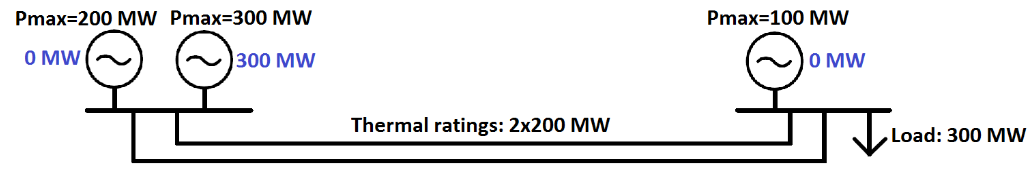
\includegraphics[width=\linewidth]{Figs/Security_vs_adequacy.png}
    \caption{Comparison of security and adequacy~\cite{adequacy_vs_security}. The system is adequate for all N-1 conditions but not operated in an N-1 secure way.}
    \label{fig:security_vs_adequacy}
\end{figure}

Adequacy thus mainly depends on the installed capacities of generators and transmission lines. Security on the other hand, also depends on how the system is operated. In this example, we assume one generator on the left bus is producing the total load of 300~MW and the other generators are turned off (typically because they are more expensive to run). 300~MW are thus transferred from the left bus to the right one. If one of the two lines suddenly fails, those 300~MW will all go through the second line that is only rated for 200~MW. That line will then likely trip (either by being disconnected by some protection system, or by heating, sagging, and entering in contact with vegetation, causing a short-circuit), separating the 300~MW generator and the load leading to a blackout (generators on the left bus no longer connected to the load, and generator on the right bus turned off and too small to satisfy the load).

This highlights an important concept for power system security that is cascading outages. In the above example, the second line is lost, not because of a defect in the line itself, but as a consequence of the loss of the first line. In this case, the loss of a single line causes a complete blackout of the system even though there was still enough generation and transmission capacity to satisfy the load.

Here, the cascading mechanism at play is the trip of lines due to overload. Depending on the severity of the overload, a line might trip after just a few seconds or after a few tens of minutes. An overloaded line can trip either because (i) one of its protection systems operates (e.g. line overload protection, distance protection), or (ii) because it overheats, sags and enter in contact with the ground or vegetation causing a short-circuit. In the latter case, power system operators might be able to relieve overloads by redispatching the system: in the example, by ramping up the power production on the right bus such that only 200~MW has to be transferred from the left one. In the former case (trip of the second line after only a few seconds), there is not enough time and only automatic corrective actions defined in advance might be able to save the system.

There are other cascading mechanisms that have overlapping time scales and can thus interact. They are strongly linked with power system stability concepts that are briefly reminded below~\cite{StabilityDefinition, StabilityDefinitionRevised} and summarised in Figure~\ref{fig:stability_classification}.

\begin{figure}
    \centering
    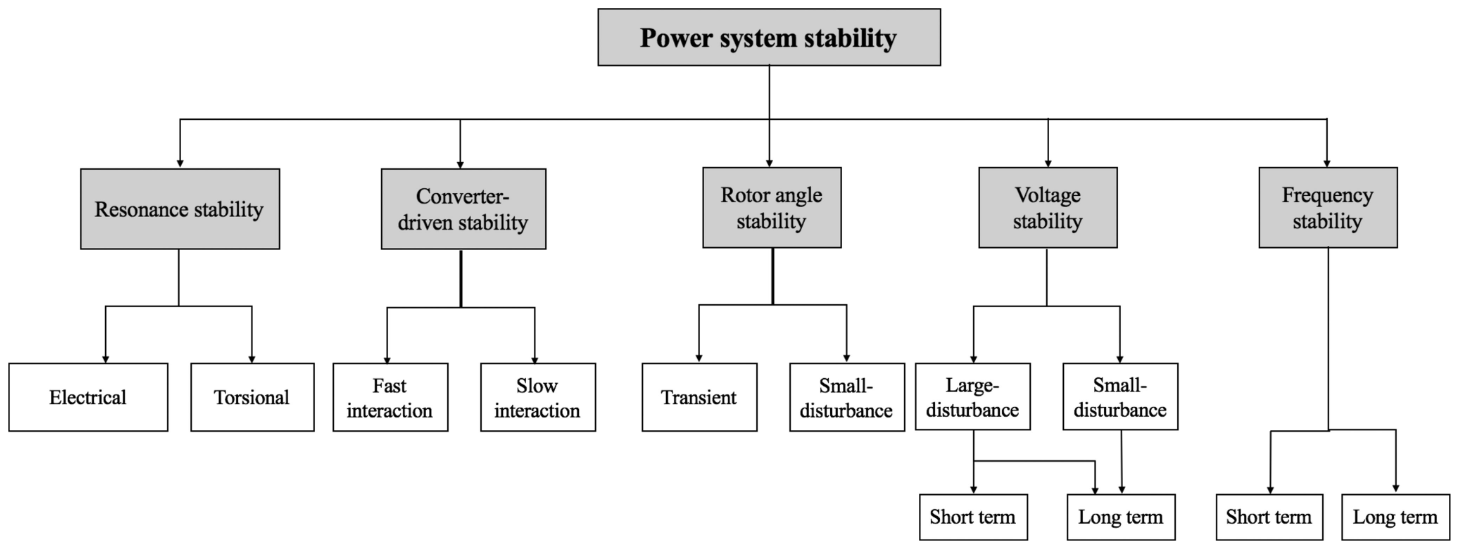
\includegraphics[width=\linewidth]{Figs/StabilityClassification.png}
    \caption{Classification of power system stability~\cite{StabilityDefinitionRevised}}
    \label{fig:stability_classification}
\end{figure}

\begin{itemize}
    \item Frequency stability is the ability of a power system to maintain a steady frequency following imbalances of load and generation. In power systems, the balance between the energy produced by generators and the energy consumed by loads should always be neutral. If there is a lack of energy produced (e.g. following the sudden loss of a generating unit), the missing energy will initially be taken from the kinetic energy of synchronous generators that will thus slow down, decreasing system frequency. If generators slow down too much, they will have to disconnect themselves to avoid damage, worsening the system imbalance and thus causing a cascading outage. For large imbalances, the inertia of synchronous generators can only maintain an adequate frequency for a few seconds. Generators thus have to quickly ramp up (or down) to stabilise the frequency. Depending on the generator technology, quick burst of production might not be sustainable, and in the longer term, the production will have to be complemented by slower ramp up of other generators and/or by turning on other generators.
    \item Voltage stability is, as the name implies, the ability of a system to maintain steady voltages close to their nominal values at all buses of the network. This ability is limited by the voltage drops that occurs when (active and/or reactive) currents flows through inductances of the transmission network. Voltage stability strongly depends on the behaviour of loads. Indeed, for a purely resistive load (e.g. electric heater), \(P = \frac{V^2}{R}\), thus if voltage decreases by 5\%, the current and power consumed by the load will respectively decrease by 5 and approximatively 10\%, helping voltage stability. If a load has a constant power behaviour (e.g. power electronics), the same voltage drop will lead to an increase in current of 5\% further aggravating the voltage drop and potentially leading to a cascade. Voltage stability is often split in short-term and long-term issues associated with the short-term and long-term behaviour of loads.
    \begin{itemize}
        \item Short-term voltage stability depends mostly on the behaviour of induction motors. When a fault occurs in a power system, low voltages arise in the neighbouring area, induction motors thus slow down as they are no longer able to generate enough electromagnetic torque to match the load torque. When the fault is cleared, motors reaccelerate, but temporarily draw additional current to do so. This can slow down the voltage recovery and even cause a voltage collapse in systems with a high share of induction motors.
        \item Long-term voltage instability occurs when loads try to restore their consumption after a voltage decrease. For example, electric heaters behave as resistive loads in the short term, so reduce their consumption when voltage decrease. However, in the long-term, this causes a decrease in temperature and thermostats thus act to return to the initial power consumption. Other important devices in long-term stability are on-load tap changers that try to recover distribution-level voltages (thus load) when transmission-level voltages are low, and over-excitation limits of generators that limit their reactive power production in the long-term to avoid overheating of the stator and/or of the rotor.
    \end{itemize}
    \item Angle stability is the ability of synchronous generators to remain in synchronism after disturbances. A machine keeps synchronism if the electromagnetic torque is equal and opposite to the mechanical torque delivered by the prime mover. Angle stability can be challenged by both small and large disturbances.
    \begin{itemize}
        \item Large-disturbance angle instability or transient instability occurs when the electromagnetic torque is insufficient which typically happens when the generator is not able to push enough electric power to the grid following loss of transmission elements and during faults.
        \item Small-signal oscillatory instability is generally caused by a lack of damping but can have many causes. Local oscillations occur when a single generator oscillates with the rest of the grid. The damping of these oscillations depend on the control systems of the generator, its power output, and the strength of the grid as seen by the generator. Global issues can be much more complex and occur when multiple generators or groups of generators oscillates against each other.
    \end{itemize}
    \item Converter-driven instability and resonance instability are new categories of instabilities that have been defined following the increasing use of power electronics (HVDC lines, FACTS devices, and inverter-based generation such as solar and wind). Power-electronic-based controls can be much faster than synchronous generator controls and can thus cause oscillations with a frequency of a dozen Hz to hundreds of kHz. As a point of comparison, frequency, voltage and angle stability are affected by phenomena with a timescale from 100ms to a few hours.
\end{itemize}

During severe disturbances, there can be interactions between different types of instabilities. For example, after the loss of a line near a large generator, voltage issues might limit the amount of power that the generator can export leading to a loss of synchronism of this generator (angle instability). The loss of this generators then causes a load generation imbalance that can lead to frequency instability.

% Fig with phenomena time ranges? (e.g. from new stability classification paper)

Due to the possible interactions between the different types of instabilities, once a cascade is initiated, it is difficult to predict how it will propagate and when it will stop. In a deterministic security assessment, this does not pose any challenge because it is considered not acceptable for the considered contingencies to lead to cascading outages. In a probabilistic assessment however, it might be acceptable for a given contingency to lead to a cascading outage, but only if the final consequences are not too big and/or if the frequency of occurrence of the contingency is sufficiently small.


\section{Deterministic security assessment}
\label{sec:traditionalSecurity}

In a traditional deterministic security assessment, a power system is deemed secure if it can withstand a set of ``credible contingencies'' without affecting customers nor violating security limits~\cite{N-1-ENTSOE}. This definition relies on three pillars that will be compared with probabilistic methodologies in the next section.

\begin{itemize}
    \item No consequences: A secured contingency should not lead to the disconnection of load nor to the violation of security limits. The definition of security limits differs from TSO to TSO, but typically require to have a steady-state voltages in an acceptable range (e.g. the voltages at all buses should be between 0.95 and 1.05pu) and the absence of equipment overload and instabilities. These security limits ensure a good power quality for end-users and normally guarantee that no cascading outage will develop (off-nominal voltages, overloads and loss of stability can all cause the trip of additional assets, leading to a cascading outage).

    Depending on the TSO, the security limits should be satisfied without the need for corrective actions (preventive approach) or after corrective actions have been implemented (corrective approach). In case (non-automated) corrective actions are used, it makes sense to define different security limits before and after the corrective actions are implemented (e.g. voltages between 0.9 and 1.1pu just after the disturbance, and between 0.95 and 1.05 after corrective actions) to make sure that the system does not cascade before corrective actions have time to be implemented.

    \item A list of credible contingencies: The set of credible contingencies is often based on the famous N-1 criterion, i.e. the power system should be able to withstand the loss of any single element (out of N). Higher-order contingencies are typically not considered because it is considered uneconomical to guarantee that they have no consequences as they rarely occur in practice.

    The N-1 criterion is not a strict religion, so contingencies might be added or removed from the list depending on the needs. For example, the loss of parallel lines located on the same tower (N-2 event) might be added to the contingency list during thunderstorm~\cite{N-1-ENTSOE}. Also, in the Nordic countries, remote areas might be operated in N-0 only as it would be too expensive to duplicate some very long lines to guarantee the security of supply of small loads.

    \item A list of pre-contingency states: To simplify the analysis, security assessment is typically performed on a small set of representative or ``umbrella states''. The set of those states should be defined according to the following criteria~\cite{CIGREreviewOfTools}.
    \begin{itemize}
        \item Credibility: the pre-contingency states should be reasonably likely to occur.
        \item Severity: the pre-contingency states considered should lead to the worst-case performance of the system for the considered contingencies.
        \item Representativity: the pre-contingency states and contingencies considered should cover the main weaknesses of the system and phenomena observed during past outages.
    \end{itemize}
    With the growing installed capacity of renewable but intermittent energy sources, it is becoming more difficult to choose a set of pre-contingency states and contingencies that simultaneously satisfy all the above criteria. Indeed, the variability of renewable energy sources greatly increases the number of possible pre-contingency system states. Consequently, the number of possible system issues also increases. If the considered set is too small or does not consider a sufficiently high variety of system configurations, important issues might be missed. On the other hand, some issues might only appear during very rare system configurations (and assuming a contingency occurs when the system is operating in such state). So, designing the system a large set of extreme cases might be uneconomical.
\end{itemize}


\section{Probabilistic security assessment}
\label{sec:probabilisticSecurity}

As opposed to deterministic methods, in a probabilistic security assessment, one does not need to make an a priori decision on what ``credible'' contingencies should be secured nor on which system states security should be assessed. Instead, probabilistic methods consider larger sets of contingencies and system states, estimate the risks associated with each scenario (combination of a contingency and initial state), and provide recommendations on how to best reduce these risks. As such, they rely less on the complex \emph{art} of defining credible scenarios, but more on the complex \emph{science} of estimating the frequency and consequences of scenarios. Also, by quantifying the risk (in terms of average energy not served to consumers (in MWh/y) or societal costs (in M€/y)), they allow for easier decision-making: what is the cost of risk mitigation measures vs. how much the risk will be decreases if those actions are implemented.

The necessity to transition from deterministic security assessment methodologies to probabilistic methodologies has been acknowledged in the industry and the literature. For example, the decision 07/2019 of the Agency for the Cooperation of Energy Regulators (ACER) of 19 June 2019 requires the European transmission system operators to develop a probabilistic approach for risk assessment of power systems by 2027~\cite{ACER}. In the literature, research on probabilistic security assessment has been active for more than two decades and is reviewed in this section.

As discussed above, probabilistic methods typically consider higher order contingencies than deterministic methods. It is thus necessary to model them and their root causes to estimate their frequency of occurrence, this is discussed in section~\ref{sec:contingencies}. Also, they consider more system states, so it is also necessary to generate these system states and to estimate their probability density function (section~\ref{sec:init_state}). Finally, for all considered scenarios (contingency and state), the potential consequences of a contingency on a given state have to be quantified. This requires to predict if a cascading outage will occur, if it does to predict how far it will propagate and what will be the final consequences for the users (in terms of energy not served or monetary cost for society). The simulation of cascading outages is thus discussed in section~\ref{sec:cascading}.

\subsection{Contingency selection}
\label{sec:contingencies}

There are many contingencies that can affect power systems, often classified using the N-x formulation, i.e. by counting the number x of elements (out of N initially available) that are lost following a contingency. Different classes of contingencies have different root causes and therefore different frequencies of occurrence~\cite{ContingencyTypes}. This section lists the main types of contingencies\footnote{Note that, as for many security-related concepts, the classification is not standardised}, explains how to estimate their frequency, and discusses the main challenges that they pose when integrating them in a probabilistic security assessment. This is also summarised in Table~\ref{tab:contingencies}.


\paragraph*{N-1 contingencies} are the simplest and the most common contingencies that can occur in power systems. They are caused by single failures of transmission or generation assets. A typical example of N-1 contingency is the loss of a line following a lightning strike on the line. N-1 contingencies are relatively frequent (not for individual assets, but on the scale of a country), so TSOs often have statistics that allow for the estimation of their frequency of occurrence. For example, in France, it is estimated that line faults occur with a frequency of 2.5 occurrences per year and per 100~km of line~\cite{FaultStatisticsFrance}. In a probabilistic security assessment, it can be noted that the frequency of occurrence of contingencies can be indirectly correlated to the system state. For example, in Finland, lightning strikes happen mostly during the summer, so system states that occur more often in the summer are more at risk. Another challenge posed by N-1 contingencies in probabilistic assessment is that, since they are relatively frequent, it must be checked that they pose little consequences in a very large majority of system states to make sure that the risk (product of frequency and consequences) they cause is acceptable.

% Often single phase faults, but consider three-phase because easier to simulate and conservative.

% \begin{table}
%     \centering
%     \caption{Summary of the categories of contingencies and the main challenges in integrating them in a probabilistic security assessment}
%     \label{tab:contingencies}
%     \begin{tabularx}{\linewidth}{@{}sslllB@{}}
%     \toprule
%     \begin{tabular}[c]{@{}l@{}}Contingency\\ type\end{tabular} &
%         Main causes &
%         \begin{tabular}[c]{@{}l@{}}Average frequency \\ of individual\\ contingencies (/y)\end{tabular} &
%         \begin{tabular}[c]{@{}l@{}}Number of\\ contingencies\end{tabular} &
%         \begin{tabular}[c]{@{}l@{}}Total\\ frequency\\ (/y)\end{tabular} &
%         Challenges \\ \midrule
%     N-1                 & Single failures      & 1    & 1000 & 1000     & High frequency \\[0.5cm]
%     N-1-1               & Independent failures & 0.00003     & 1,000,000 & 30 & Number of contingencies \\[0.5cm]
%     N-k (k = 2-5)       & Common-mode and hidden failures & 0.01 & 10,000 & 100   & Modelling of causes \\[0.5cm]
%     N-1 (delayed clearing) & Hidden failures & 0.1 & 1000 & 100   & Intermediate between N-1 and N-k \\[0.5cm]
%     N-K (K \(\gg\) 2)   & Hurricanes, earthquakes, cyber-attacks & Variable  & Variable & Variable & Modelling of causes and restoration \\[0.5cm]
%     Other contingencies & Black clouds              & N/A    & N/A & N/A & Modelling of causes \\ \bottomrule
%     \end{tabularx}
%     \end{table}

\afterpage{%
\clearpage% Flush earlier floats (otherwise order might not be correct)
% \thispagestyle{empty}% empty page style (?)
\begin{landscape}% Landscape page
\centering
\begin{table}
\caption{Summary of the categories of contingencies, order of magnitude of their frequency and number (for a system with 1000 branches), and main challenges in integrating them in a probabilistic security assessment}
\label{tab:contingencies}
\begin{tabularx}{\linewidth}{@{}lslllB@{}}
\toprule
\begin{tabular}[c]{@{}l@{}}Contingency\\ type\end{tabular} &
    Main causes &
    \begin{tabular}[c]{@{}l@{}}Average frequency \\ of individual\\ contingencies (/y)\end{tabular} &
    \begin{tabular}[c]{@{}l@{}}Number of\\ contingencies\end{tabular} &
    \begin{tabular}[c]{@{}l@{}}Total\\ frequency\\ (/y)\end{tabular} &
    Challenges \\ \midrule
N-1                 & Single failures      & 1    & 1000 & 1000     & Security must be guaranteed for a large set of system states \\[0.5cm]
N-1-1               & Independent failures & 0.00003     & 1,000,000 & 30 & Very high number of possible contingencies, but most do not pose security risks \\[0.5cm]
N-k (k = 2-5)       & Common-mode and hidden failures & 0.01 & 5000 & 50   & Modelling of common-mode and hidden failures \\[0.5cm]
N-1 (delayed clearing) & Hidden failures & 0.1 & 1000 & 100   & Intermediate between N-1 and N-k \\[0.5cm]
N-K (K \(\gg\) 2)   & Hurricanes, earthquakes, cyber-attacks & Variable  & Variable & Variable & Modelling of the causes of contingencies and of the recovery of the system after contingencies \\[0.5cm]
Other disturbances & Black clouds              & N/A    & N/A & N/A & Modelling of the causes of contingencies \\ \bottomrule
\end{tabularx}
\end{table}
\end{landscape}
\clearpage% Flush page
}

\paragraph*{N-1-1 contingencies} are a combination of two N-1 contingencies that occur in relatively quick succession. Power systems are typically designed to be N-1 secure. However, once an N-1 contingency occurs, the system can degrade to an N-0 secure state. When this happens, operators will try to perform corrective actions to bring back the system to an N-1 state. But if a second contingency happens before operators have time to act, it might challenge system security. If contingencies are assumed to be independent, the frequency of an N-1-1 contingency that consist in contingency \(i\) occurring after contingency \(j\) but after a time less than \(T\) is

\begin{equation}
\label{eq:N-1-1_frequency}
    f_{i,j} = \lambda_i  (1-e^{-\lambda_j T})
\end{equation}
\noindent where \(\lambda_i\) is the frequency of occurrence of contingency \(i\), and \((1-e^{-\lambda_j T})\) is the probability that contingency \(j\) occurred in the last \(T\) minutes. In static security assessments (i.e. assessments that consider asset ratings (and steady-state voltage limits), but not dynamic stability issues), such contingencies can be considered as N-2 contingencies as they have the same effect. This is not the case in dynamic security assessments, because the time delay between the occurrence of the two contingencies usually makes the N-1-1 contingency less severe than if the two contingencies occurred at the same time. N-1-1 contingencies that occur with significant time delay between the two contingencies (i.e. leaving enough time to perform corrective actions) can also be considered to check that it is indeed possible to bring back the system to an N-1 secure state after a first contingency. (This is mostly done in static security assessments, for example in the US~\cite{ContingencyTypes}.)

Individual N-1-1 contingencies have an extremely low frequency of occurrence but many possible N-1 contingency combinations are possible leading to a very high number of possible N-1-1 contingencies. Indeed, from (\ref{eq:N-1-1_frequency}), if two contingencies have a frequency of 1 per year, and if we assume that it takes on average 15 minutes for operators to bring back the system to an N-1 secure state (\(T = 15 \text{ minutes}\)), then these two contingencies will lead to N-1-1 conditions every 30 per \emph{million} years. But, if there are \(N = 1000\) possible N-1 contingencies, there are \(N(N-1) \approx 1,000,000\) possible N-1-1 contingencies. So, in total, N-1-1 contingencies would happen 30 times per year in this example. This is the same order of magnitude as the total frequency of N-k events (see Table~\ref{tab:contingencies} and next paragraph)\footnote{In~\cite{ContingencyMotifs}, authors analysed 19 years of historical outage data recorded in the Bonneville Power Administration power system and observed that when two lines failed in a one-hour interval, in 81\% of the cases, the two lines were adjacent, indicating an N-k contingency (or small cascade).}, however, on average, N-1-1 contingencies have less chance to have consequences than N-k contingencies. Indeed, especially in large systems, two N-1 contingencies occurring at opposite ends of the system will unlikely lead to consequences. The risk of independent N-1-1 contingencies can thus often be neglected compared to N-k contingencies. But if they are considered anyway, screening techniques should be used to limit the number of combinations to simulate~\cite{VittalN-1-1}.

N-1-1 contingencies can become much more likely when they are no longer independent. For example, in 2021, two parallel interconnections between France and Spain where lost at two minutes of interval due to a wildfire. This initiated a cascade that led to the separation of the two systems~\cite{ENTSOEIbericSplit2021}. The system should have preventively been made N-1-1 secure in the vicinity of the fire to avoid this incident, but system operators were unaware of the fire due to lack of communication from the fire department.


\paragraph*{N-k contingencies (k = 2-5)} consist in the simultaneous loss of k elements. N-k contingencies virtually cannot occur due to independent contingencies (limit of \(T \to 0\) in (\ref{eq:N-1-1_frequency}) gives a null frequency), and instead occur due to common mode and hidden failures. A common mode failure is the simultaneous failure of several elements due to a single root cause. For example, two lines sitting on the same tower will be lost if the tower is lost. Also, busbar faults are often considered to be N-k contingencies because all lines connected to the busbar might need to be disconnected to clear the fault. As seen from those examples, N-k contingencies often imply the loss of elements located in close proximity (parallel lines, adjacent lines) and are thus often more severe than N-1-1 contingencies.

A hidden failure is a failure that does not directly impact system operations but increase the chance of failure of equipment to perform an on-demand function. Hidden failures are of particular concern in protection systems. Indeed, protection systems need only to operate when a fault occurs in a given element of the grid. If a protection system fails, a backup protection system will need to operate to clear the fault and avoid equipment damage. Backup protections are however slower than primary protection and often trip multiple non-faulted elements. Protection systems and their failure modes will be discussed in much more details in chapter~\ref{ch:protections}.

% Mention Ian Dobson paper \url{https://ieeexplore.ieee.org/stamp/stamp.jsp?arnumber=10054456}, \url{https://arxiv.org/pdf/2209.02192} but (identified) critical lines might have more reliable protections (e.g. double differential (independent sets of relays), or even SIPS) than less critical ones (e.g. single distance protection with overcurrent backup). (Time resolution of data (1min) makes it difficult to differentiate between independent events and cascade. Actually, probably need some manual postprocessing to separate the two)

The importance of hidden failures is highlighted by the study of historical blackouts. For example, Ref.~\cite{CascadingMethodoAndChallenges} observed that out of the 26 major unreliability events reviewed in a CIGRE (Conseil international des grands réseaux électriques) report\footnote{Most of these disturbances affected more than one million customers and led to at least 5~GW of power not served}~\cite{majorBlackouts}, 19 of them were triggered by losses of single transmission elements albeit many of these events were exacerbated by other problems. Further analysis shows that 18 of the 26 events were caused or aggravated by hidden failures. The same observation can be made for smaller scale events. For example, the study of significant disturbances reported by the NERC~\cite{NERCDisturbancesReport} (North American Electric Reliability Corporation) in the period from 1984 to 1988 and summarised in~\cite{ZoneVulnerability} indicates that protective relays misoperations were involved, in one way or another, in 73.5\% of disturbances\footnote{This includes both spontaneous operation of protections (without preceding event) and hidden failures. However, as power systems are designed to be N-1 secure, spontaneous operations should usually not have consequences.}.

More complex phenomena can also lead to N-k contingencies. For example, in 2019, a fault occurred on a 400kV line in the UK and was normally in 80ms. But then, a wind farm located roughly 200 km away from the fault rapidly decreased its production from 799 to 62~MW. Shortly after, a steam generator (located close to the initial fault) was disconnected. This led to a large generation load imbalance that, along with other aggravating factors, led to a frequency decrease and to the disconnection of one million customers~\cite{2019UKBlackout}. It is extremely difficult to predict such events and to estimate their frequency. However, following a growing number of cases where generators failed to ride through normally cleared transmission faults (which is a requirement for any transmission-connected generator), the UK grid codes were updated such that generators that failed to meet fault-ride through requirements have to limit their production (possibly to 0~MW, to limit the threat they pose to system security) until they are able to demonstrate that they meet the grid codes~\cite{FaultRideThroughEnforcement}. Such issues should therefore become rarer, at least in the UK.


\paragraph*{N-1 contingencies with delayed fault clearing} are similar to N-k contingencies in that they are caused by a single fault that is not cleared by the primary protection system of the faulted element. The difference is that the backup is able to clear the fault by disconnecting only the faulted element (but still requires more time than the primary protection to do so). They are often more likely than N-k contingencies (less severe failure of protection system) but have a smaller impact on the system\footnote{No publicly available statistics were found regarding the rate of N-1 contingencies with delayed fault clearing. The frequency of 0.1/y in Table~\ref{tab:contingencies} is thus taken as an intermediate between the one of normal N-1 contingencies and the one of N-k contingnecies}. Their relative contribution to the total risk thus depends on the considered power system.


\paragraph*{N-K contingencies (K \(\gg\) 2)} are caused by extreme events such as hurricanes, earthquakes (weather events) and cyber-attacks (man-made events). Such extreme events have a low frequency but can lead to the loss of many assets in a short period of time. The ability of power systems to withstand such events falls out of scope of the topic of security (thus of this thesis) to the one of resilience. Apart from the larger severity of such events, another difference with security-related events is that it is more difficult for the system to recover from them. Indeed, security-related events can lead to cascading outages and even complete blackouts, but rarely cause damage in transmission equipment and generators. Black start and complete restoration is usually performed in less than 24~hours. While for extreme events, parts of the network might stay deenergised for days or weeks before the necessary repairs can be completed.


\paragraph*{Other disturbances} are disturbances that do not fall in the above categories. One example of such disturbance is the occurrence of black clouds. (Moving) black clouds can cause large and relatively fast changes in power flows by obscuring photovoltaic panels and causing increased load (lighting, heating), especially when above large cities. Such disturbances weaken the system and can lead to large consequences, especially when combined with the above contingencies. They are not very well documented and thus not considered further in this thesis.

% specific analyses, can go outside the purely probabilistic framework (e.g. sensitivity)


\subsection{Generating likely system states}
\label{sec:init_state}

To evaluate the risk associated with a given contingency, it is necessary to predict in what initial state the system could be upon occurrence of the contingency and what are the probabilities of all possible initial states. Mathematically speaking, this requires to have (an approximation of) the probability density function of the system state\footnote{Actually, it would be best to have a probability density function conditioned by the occurrence of the contingency to account for correlations between the occurrence of a contingency and the system state (e.g. in Belgium, lightning strikes are more likely to occur during the summer when the load is low)} (generator outputs, load flows, asset availability, etc.).

Estimating this probability density function is very challenging because it is a high-dimensional function (must account for (active and reactive) power injection at all buses, asset availability, substation topologies) with strong correlations between its variables (especially spatio-temporal correlations between the renewable energy availability at different points in the network). Despite the importance of this step in the probabilistic security assessment work, it has not been studied in details in this thesis. Instead, two of the most potent and popular methods from the literature are described below. The former will be used in the test cases in section~\ref{ch:DPSA}.

The first method has initially been developed in the GARPUR project~\cite{StrathElia, StrathGARPUR} and is now routinely used by some European TSOs and ENTSO-E to perform adequacy studies~\cite{ACER_MC_year, EliaAdequacy}. The methodology consists in, first, using weather data to generate so-called ``Monte Carlo (MC) years''. An MC year is time series realisation of renewable generation availability and load for one year with a typical resolution of one hour. Please refer to~\cite{StrathGARPUR} for more information on how to generate MC years while considering temporal and geographical correlations between renewable outputs and loads. Secondly, for each MC year, a market model is used to determine the commitment of thermal generators. Finally, each year is divided into (e.g. hourly) snapshots, and a (security-constrained) optimal power flow is performed on each snapshot to model potential preventive actions taken by operators. All snapshots are saved in a database to be used in the rest of the probabilistic security (or adequacy) assessment. % (\cite{DCAT_2023} also uses weather, but few details given)

The second method consists in fitting an analytical probability density function based on historical data, often using copula to handle correlations. This approach has been extensively studied during the iTesla project~\cite{KonstantelosCopulas, EurostagHPC}. In this project, the complete system state, including substation topologies (and accounting for potential preventive actions performed by operators), was directly inferred from historical data. This can be more accurate than the GARPUR approach, because optimal power flows do not handle well substation topologies (requires many binary variables in the optimisation problem) and operator actions (do not always perform the predicted optimal actions). However, the reliance on historical data makes it a less flexible approach. In particular, it does not allow to model the impact of climate change on the likelihood of droughts and other severe weather events. So it is less adequate for long-term (e.g. 10 year horizon) studies. Also, if operating rules are modified (e.g. to enhance security as we will discuss in chapter~\ref{ch:DPSA}), historical data on operator actions might no longer be relevant.

% One industry-grade tool worth mentioning is ASSESS~\cite{AssessRTE, AssessNationalGrid} developed by RTE and National Grid (i.e. the French and British TSOs respectively). It does not compute the consequences of contingencies (i.e. only classify them as acceptable or not), but it generally considers more uncertainties in the pre-contingencies states, and it has a toolbox of statistic and data mining tools that can be used to analyse the results. It is particularly useful to define operational limits by ``drawing a line'' between the acceptable and unacceptable pre-contingencies states. % Little information given (except many probability laws are available --> No correlations?)


\subsection{Simulation of cascading outages}
\label{sec:cascading}

For each combination of initial system state and contingency (called a scenario hereafter) considered in the analysis, it is necessary to quantify what would be the impact of the contingency if it occurred when the system was in the considered initial state. For the scenarios that lead to cascading outages, it can be challenging for two main reasons. The first is that simulating cascading outages requires to simulate the system in very degraded states. This is not needed in deterministic security assessments and thus rarely done by TSOs. Models are thus poorly validated in those degraded states. Moreover, power systems rarely face very degraded states, so there might be a lack of data to validate the models.

The second challenge is that, in some cases, cascading outages might be very sensitive to modelling assumptions. This is because in a cascading outage, many elements are subject to abnormal conditions and thus likely to trip or misoperate. A good example of this is the tripping of lines caused by overload. When a line is overloaded, its temperature increases due to the Joule effect. It thus sags and can then enter in contact with vegetation causing a short-circuit followed by a trip of the line. The line trip causes a redistribution of the power flows and can cause overloads in other lines which contribute to the propagation of the cascade. The redistribution could also resolve some overloads, stopping the cascade propagation. At some point in the cascade, it is likely that multiple lines will be overloaded. In the first probabilistic security assessment methodologies developed, a common assumption was that, in case of multiple overloaded lines, the most overloaded line would trip first. In practice however, slightly less overloaded lines could trip first due to different vegetation height, weather, etc. The trip of a different line can cause a very different redistribution of power flows that causes different lines to be overloaded in the next step of the cascade. The resulting cascade can thus be very different (in terms of size, geographical distribution, impacted elements, etc.) than the one where the most overloaded line was tripped first. This difference is further amplified when we consider the competition between different cascading mechanisms.

In the literature, two main types of methods have been developed to simulate cascading outages: the ones based on a static grid model (section~\ref{sec:QSSmethods}), and the ones based on a dynamic grid model (section~\ref{sec:DynMethods}). These methods are quite different as they have to cope with different limitations. The former have to introduce additional heuristics to approximate dynamic effects while the latter are limited by computation time. Additionally, some methods do not fall in the above categories and are reviewed in section~\ref{sec:OtherMethods}.


% Actually, a lot of different methodologies can be placed under the umbrella of probabilistic methodologies, but the number of uncertainties taken into account can vary greatly. The most straightforward probabilistic assessment method is the contingency enumeration method. It is similar to the deterministic method in that one will assess the security of a list of contingencies (usually larger than in a deterministic assessment, e.g. including N-2 events and loss of towers). The difference is that contingencies are associated with a probability. Also, instead of simply classifying contingencies as acceptable or unacceptable, the consequences are usually computed, but in a deterministic manner. Due to the relative simplicity of the methodology and similarity with the deterministic method, it is implemented in most commercial software tools\footnote{At the time of the writing of the CIGRE review~\cite{CIGREreviewOfTools} (2010), all tools used the quasi-steady-state (QSS) approximation (that will be described in section~\ref{sec:QSSmethods}) to evaluate the consequences. Now, some tools (e.g. PSS/E~\cite{PSSE} and DIgSILENT PowerFactory~\cite{PowerFactory}) also allow to use dynamic simulations. Due to the simplicity of the method, it is possible to implement it with any tool that has basic scripting functionality.}~\cite{CIGREreviewOfTools}.

% Industry-grade tools only consider the uncertainties related to the initial state and initial contingencies. After the occurrence of a given contingency, the system is simulated in a fully deterministic manner. Those tools are thus unable to consider hidden failures as those manifest after the initial contingency\footnote{The hidden failures that occur just after the initiating event (e.g. failure to open a faulted line) could be modelled as part of the initiating events as done in~\cite{Haarla, GridPSA}. This is discussed in section~\ref{sec:DynMethods}. This is however not possible for failures that occur later in the cascade. For those, it is necessary to have a probabilistic simulation of the evolution of the cascade.}.




\subsubsection{Methods with a static grid model}
\label{sec:QSSmethods}

Methods based on a static grid model typically follow a common scheme illustrated in Figure~\ref{fig:QSS_flowchart}. First, the system is initialised at the pre-contingency state, and the initiating contingencies are triggered. Then, the post-contingency state is computed using an (AC or DC) power flow algorithm. If some elements are subject to unacceptable conditions (e.g. overload, undervoltage, etc.), those elements are tripped or other remedial actions are implemented (e.g. under-voltage load shedding (UVLS), redispatch, etc.). After those disconnections/actions, the state of the system is recomputed. The process is repeated until no more elements are subject to unacceptable conditions or if a full blackout occurs.

\begin{figure}
    \centering
    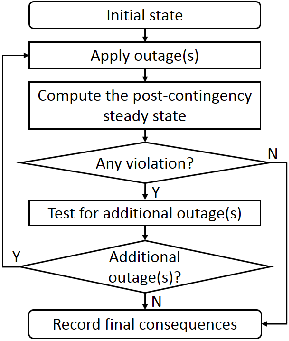
\includegraphics[width=0.4\linewidth]{Figs/QSS_flowchart.pdf}
    \caption{Typical flowchart of static cascading outage methodologies~\cite{Benchmarking2018}}
    \label{fig:QSS_flowchart}
\end{figure}

As the computation cost of a power flow is relatively low (of the order of 1s for large systems), the cost of static methods is also low. This is particularly useful as probabilistic security assessment methodologies require to simulate many scenarios. An obvious limitation is that static methodologies do not directly account for stability issues as they do not perform time-domain simulations. Historically, this was justified by the fact that cascading outages used to often develop in two phases: a slow phase driven by thermal phenomena (line overloads) followed by a fast phase driven by stability issues (frequency, loss of synchronism, etc.). Figure~\ref{fig:BlackoutUS2003} demonstrates this for the case of the 2003 US blackout~\cite{USBlackout2003}. The cascade was initiated at 15:05 by the loss of multiple parallel lines due to heavy loading. One hour later (at 16:05, start time of Figure~\ref{fig:BlackoutUS2003}), two dozen lines were disconnected. Around 16:09 the cascade transitioned to a fast phase and hundreds of elements were disconnected in two minutes. In the light of this blackout, static methodologies are often seen as adequate to model the early stage of cascades, but not their fast phase (where most of the elements and loads are disconnected)~\cite{BenchmarkingStaticVsDynamic}. This has led to the development of hybrid methodologies where the start of cascades is represented with a static model, and the end with time-domain simulations~\cite{TwoLevelPSA, DCATphase1}.

\begin{figure}
    \centering
    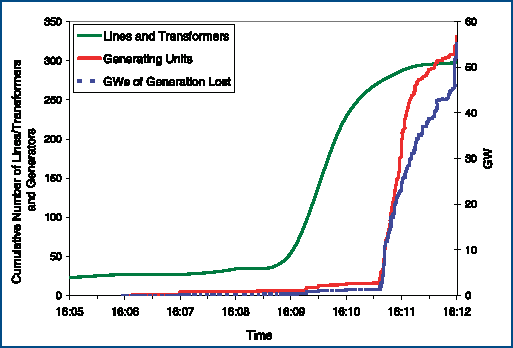
\includegraphics[width=0.7\linewidth]{Figs/USBlackout2003.pdf}
    \caption{Rate of line and generator trips during the cascade that led to the 2003 US blackout~\cite{StabilityDefinitionRevised}}
    \label{fig:BlackoutUS2003}
\end{figure}

A major challenge in the simulation of cascading outages is the handling of ``race conditions''. For example, if at a given step of the cascade, two lines are overloaded, which of the two lines will trip first? Actually, will they trip at all, or will an operator be able to relieve the overloads before lines are tripped? Such race conditions can also occur between different types of cascading mechanisms (e.g. will the overloaded line trip before the over-excitation limiter of a generator acts).

% This depends on whether the lines were already overloaded in the previous cascading steps and on variables (weather, vegetation height) that are difficult to model. This race conditions can also occur between different types of cascading mechanisms (e.g. will the overloaded line trip before the over-excitation limiter of a generator acts). The handling of these race conditions is made even harder by the fact that QSS simulations have no concept of time (as load flows assume the system is in steady-state).

Handling of race conditions can be performed with either single-path or multi-paths methods. In the former, only the most likely (estimated) cascading path is simulated. For example, some cascading failure simulators consider that when multiple lines are overloaded, the most overloaded one will trip first. Others trip all overloaded lines in one step~\cite{ManchesterNoebels}. In the multi-path, multiple cascading paths are simulated, each associated with a probability and specific consequences. The probability of an overloaded line to trip is often estimated as a function of the current overload value and/or as a function of the line temperature (computed based on past values of the line currents and on weather)~\cite{Henneaux_level1}.

Another important issue in cascading simulators based on static grid models is the handling of cases where the power flow does not converge (only if AC power flow model is used and/or if discrete controls such as tap changers are included in the power flow model). Non-convergences are often caused by voltage issues and thus resolved by shedding load until the power flow converges or using an optimal power flow to find the minimum amount of load shedding necessary to get convergence. In a dynamic simulation, voltage collapses occur in a ``smoother'' manner as voltages are explicitly considered as time-dependent continuous variables. One can thus observe e.g. which loads are subject to undervoltages first and thus which tap changers or under-voltage load shedding relays will actually trigger and in which order\footnote{Numerical stability issues can also occur in dynamic simulations but they tend to be rarer. To avoid those issues, one should be cautious of the models used (e.g. Ref.~\cite[p93-98]{SongThesis} proposes to replace constant-power loads with restorative loads with a very short time constant). Protections tend to mitigate numerical issues as they disconnect elements are subject to severe conditions (e.g. distance protections disconnecting lines during voltage collapse).}.


% To better illustrate QSS methodologies and the challenges they face in modelling race conditions and stability issues, an example of QSS methodology is described and discussed. The example considered is the AC cascading failure model (AC-CFM)~\cite{ManchesterNoebels} that can be considered as one of the spiritual successors of the famous Manchester model~\cite{OriginalManchesterModel}. This model follows a similar procedure to most QSS models, that is it initialises the system, triggers an initiating contingency, and then checks for violations and performs corrective actions until all violations are solved. The steps that are taken to solve violations at a given step of the cascade are illustrated in Figure~\ref{fig:NoebelsFlowchart} and discussed below.

% \begin{figure}
%     \centering
%     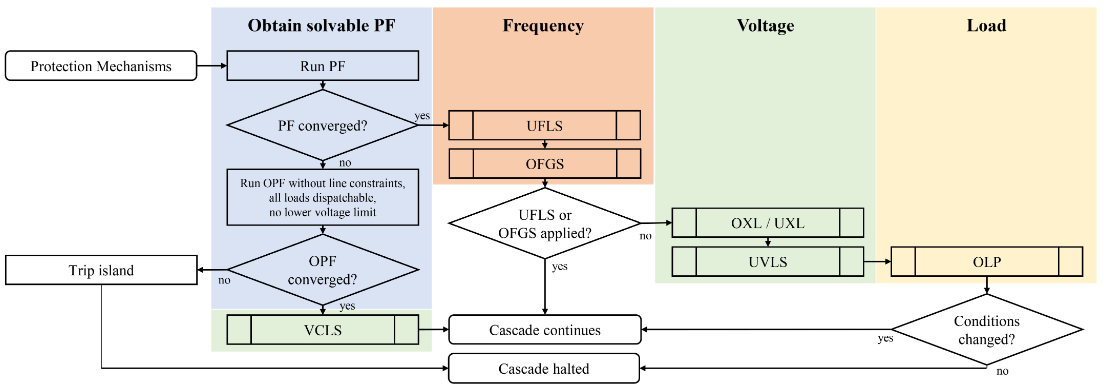
\includegraphics[width=\linewidth]{Figs/NoebelsFlowchart.png}
%     \caption{Flowchart of the AC-CFM methodology~\cite{ManchesterNoebels}. Abbreviations: PF: power flow, VCLS: voltage collapse load shedding, UFLS: under-frequency load shedding, OFGS: over-frequency generator shedding, OXL/UXL: over/under-excitation limiter, UVLS: under-voltage load shedding, OLP: overload protection}
%     \label{fig:NoebelsFlowchart}
% \end{figure}
%
% \begin{itemize}
%     \item Obtain a solvable power flow: AC-CFM uses an AC power flow and AC power flows can fail to converge. This is often caused by lack of reactive power support that causes a voltage collapse. The modelling choice made for the AC-CFM is to use an OPF considering all loads are dispatchable, and to minimise the load shedding necessary to obtain a converging load flow. In a dynamic simulation, voltage collapses occur in a ``smoother'' manner as time is explicitly considered as a continuous variable. One can thus observe e.g. which loads are subject to undervoltages first and thus which UVLS relay actually triggers\footnote{Numerical stability issues can also occur in dynamic simulations but they tend to be rarer. To avoid those issues, one should be cautious of the models used (e.g. Ref.~\cite[p93-98]{SongThesis} proposes to replace constant-power loads with restorative loads with a very short time constant). Protections tend to mitigate numerical issues as they disconnect elements are subject to severe conditions (e.g. distance protections disconnecting lines during voltage collapse).}.
%     \item Frequency: AC-CFM considers that if load-generation imbalances are less than a predefined threshold, the imbalance will be redistributed to the generators (that will increase or decrease their power to restore the imbalance) according to their participation factors. For larger imbalances, load shedding or generation rejection is necessary. In case of lack of generation, the load is reduced uniformly (although prioritisation can be implemented). In case of generation surplus, generating units are disconnected starting with the smallest ones as they tend to more easily lose synchronism. When using dynamic simulations, frequency is modelled explicitly, so it is easier to model the response of generators and to predict when under-frequency load shedding (UFLS) thresholds are reached.
%     \item Voltage: this block has two parts: the over/under-excitation limiters of generators, and UVLS.
%     \begin{itemize}
%         \item OXL/UXL: in AC-CFM, generators that are over/under-excited are made into PQ buses, i.e. their reactive power output is considered equal to its limits. In a dynamic simulation, limiters could be modelled similarly. However, as over-excitation limiters protect the generators against excessive heating, a time-delay can be considered. It is also easier to consider the variation of reactive limits with the active power output.
%         \item UVLS: in AC-CFM, load is shed by block until voltages reach acceptable values. If multiple loads are subject to undervoltages, load is shed in all of them simultaneously. In a dynamic simulation, the order of triggering of UVLS relays will depend on the time evolution of voltages at individual load buses. UVLS at one bus can then alleviate or worsen voltage issues in neighbouring buses.
%     \end{itemize}
%     \item Load: in AC-CFM, overloaded lines are tripped. If multiple lines are overloaded, they are all disconnected. In dynamic simulations, the order of tripping can be better modelled. Also, lines can also be tripped by distance and out-of-step protection relays.
% \end{itemize}
%
% The above points are considered sequentially in each step of the cascade in the AC-CFM model. In other words, AC-CFM considers that frequency issues are solved first, followed by voltage issues, then overload issues. Again, in a dynamic simulation, the order and interactions between those issues can be better modelled. Finally, angle stability issues are not considered in AC-CFM.

Due to the different modelling assumptions used by different static cascading simulators, different simulators can give significantly different results. Moreover, there is currently no consensus on the details of modelling required for static cascading failure simulation~\cite{Benchmarking2018, BenefitsAndChallengesDynamicPreece}. And benchmarking has shown that different static methodologies lead to different results in terms of cascade size distribution (with differences of more than one order of magnitude as shown in Figure~\ref{fig:QSS_ccdf}), total expected demand loss, and identified critical components.

\begin{figure}
    \centering
    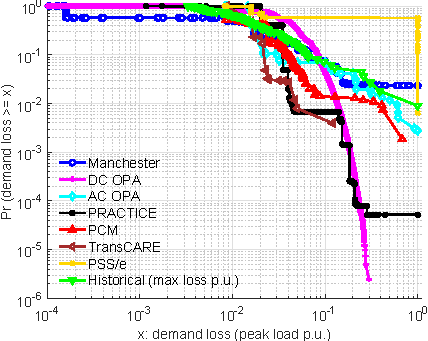
\includegraphics[width=0.6\linewidth]{Figs/QSS_ccdf.pdf}
    \caption{Comparison of the blackout size probabilities predicted by different QSS methodologies~\cite{Benchmarking2018}}
    \label{fig:QSS_ccdf}
\end{figure}

It is interesting to note that, outside the field of cascading outage analysis, there has also been some concerns regarding static grid models. For example, RTE (the French TSO) is developing a tool called DynaFlow for steady-state computations using simplified time-domain simulation. Steady-states are usually computed with a power flow algorithm. But, additional loops are needed to account for controls used in power systems (e.g. on-load tap changers, phase-shifter transformers, etc.). The order or which those loops are applied has an impact on the final state that is computed. This order was previously defined using heuristics and experience, but this was becoming complex with the increasing number of loops, especially for large systems (and power systems becoming more ``smart''). DynaFlow showed more accurate results and ease of use~\cite{DynaFlow}. A similar tool called DynaWaltz was developed for long-term voltage stability~\cite{DynaWaltz}. % This tool replaced their previous QSS tool. DynaWaltz showed better accuracy than its predecessor while keeping similar computation times~\cite{DynaWaltz}.



\subsubsection{Methods with a dynamic grid model}
\label{sec:DynMethods}

Methods based on a dynamic grid model use time-domain simulations to assess the consequences of a given scenario. In this thesis, time-domain simulations are considered to be of the root-mean-square (RMS) type. Indeed, probabilistic security assessment methodologies based on RMS simulations are already strongly limited by computation time and thus cannot afford to use electromagnetic transient (EMT) simulations. The need for EMT simulations is driven by the increasing penetration of converter-interfaced generation (wind, solar), load (electric vehicle chargers), and transmission elements (HVDCs, STATCOMs, etc.) that have very fast dynamics (bandwidth from a dozen of Hz up to hundreds of kHz). Power electronics can cause oscillations at these high frequencies and impact system stability. Modelling these oscillations requires the use of EMT models. However, actions to avoid these oscillations can largely be taken at the local (plant) level~\cite{AvoidEMT}. Also, grid-forming controls of power electronics can be used to limit the loss of system inertia caused by the decreasing share of synchronous generator~\cite{GridFormingAreTheyTheKey}. It is thus expected that RMS simulations will remain adequate to simulate \emph{system-wide} disturbances at the system level for most scenarios. Screening indicators could be used to identify the scenarios for which it is not the case. Co-simulation with RMS and EMT tools (simulating part of the grid with EMT and part with RMS) could also be used to alleviate the computational burden of EMT simulations.

The main advantage of time-domain simulations is that they allow for a conceptually easier modelling than static cascading simulators. Actually, the only additional challenges of using time-domain simulations in a probabilistic security assessment compared to a deterministic one are that (i) the system is simulated further from normal operations, challenging the accuracy of the models, and (ii) protection systems (and their possible failures and misoperations) play a much more significant role and need to be modelled explicitly. Sensitivity studies are very important to control the first point, and chapter~\ref{ch:protections} is dedicated to the second.

The drawback of dynamic methods is significantly larger computation times and data requirements. Compared to static methods, the additional necessary data are mainly linked to (i) the dynamic models of generators, loads, etc. and (ii) the models of protections. Data for the first point is generally available to TSOs as stability studies are performed routinely, but the validity of existing models might be challenged when simulating the system during severe disturbances.  The second point requires data regarding the failure modes and failure rates of protection systems (that can be difficult to estimate) and the protection settings (that should be available but introduce additional data handling issues).

Moreover, using time-domain simulations does not resolve the fact that cascading outages can be very sensitive to modelling uncertainties and in particular to the timing of protection system operations. Multi-paths methods are still needed to handle this issue. Different techniques have been developed in the literature and are reviewed below.

In~\cite{SongThesis, SongPaper, Preece1000RandomDynN-2}, protections systems are modelled as perfectly reliable: they never fail and always trip at the expected threshold. This is thus does not consider the sensitivity of cascading outages and does not allow for the consideration of N-k outages caused by protection failures. N-1-1 contingencies were considered instead (although referred to as N-2 contingencies).

The Pacific Northwest National Laboratory (PNNL) developed a tool called Dynamic Contingency Analysis Tool (DCAT) for security assessment of power systems~\cite{DCATphase1, DCATphase2}. In this tool, after the initiating contingency, the evolution of the system is computed using dynamic simulation. Protections are modelled explicitly in the simulation, and when one protection activates, the simulation is stopped and the state of the system is saved. From this save, two simulations are run, one where the protection actually operates, and one where it fails to (representing failure of a circuit breaker to open on demand). The limitation of this method is that only missing protection operations are considered. Unwanted operations are not considered. Also, the sensitivity of cascading outages is not considered. Moreover, the reports did not show any example of application using the ``protection misoperation'' functionality. There was also no discussion on the impact on the computational burden of this feature. But, in~\cite{DCAT_2023}, it is shown that it takes around one day with a 24-core computer to simulate 1465 scenarios (combination of an initial system state and contingency) on the WECC system (west US) using DCAT. The scenarios consisted in a combination of 2 contingencies with around 600 system states and in a combination of 213 contingencies with 1 system state. It was not possible to perform a systematic analysis with both many contingencies and many system states.

A particularity of DCAT is that is uses both dynamic and static simulations. Indeed, it uses dynamic simulations for the first 30 to 60 seconds after the initial contingency. If the system is deemed dynamically stable (i.e. if no event occurs during the last dozen of seconds of the dynamic simulation), the tool then switches to (single-path) static simulation. When an event occurs in the static simulation (e.g. a corrective action), the tools switches back to dynamic simulation. This allows for the simulation of the system over long time scales (minutes to hours to account for e.g. line overloads) with reasonable computation time while still accurately simulation faster phenomena (e.g. frequency stability in the 100ms-10s range). Another way to achieve this is via the use of time-domain simulators with a variable integration time-step such as Eurostag~\cite{STAG}.

Ref.~\cite{Haarla, GridPSA} proposed a methodology based on event trees. An example of event tree is shown in Figure~\ref{fig:eventTree}. An event tree starts at a given initiating event (a permanent line fault in the left of the figure). The event tree then branches when subsequent events (typically protections against the initial event) are possible. Upward branches are usually associated with the occurrence of an event (e.g. protection operates successfully), and downward branches with the non-occurrence of the event (e.g. protections fails to operate). The event tree thus generates a number of scenarios whose frequency and consequences can be estimated. The frequency of a branch is computed as the frequency of the initial event multiplied by the probability of the subsequent (non-)events. To complement event trees, fault trees can be used to model common-mode failures, they are presented in more details in dedicated literature~\cite{FaultTreeHandbook}. Consequences are estimated using dynamic simulations. The limitation of this method is that the event tree is built prior running the simulations. The analyst thus has to predict which protections will be activated. In practice, this is only possible for the protections that isolate the fault (e.g. protections at both sides of the line and backups for these protections). This method only allows to consider some protection failure modes (although it is quite good at it). Also, in this case, the sensitivity of cascading outages was not considered.

\begin{figure}
    \centering
    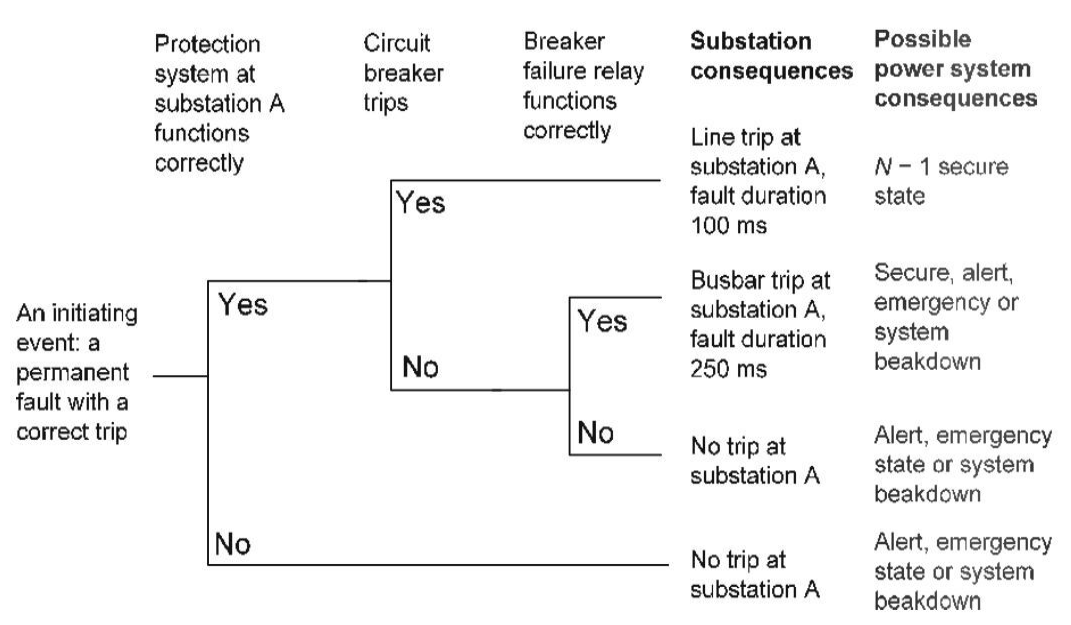
\includegraphics[width=0.8\linewidth]{Figs/EventTree.png}
    \caption{A simplified example of event tree for a line short-circuit~\cite{GridPSA}}
    \label{fig:eventTree}
\end{figure}

In~\cite{TwoLevelPSA, Faghihi}, an extension of event trees called dynamic event trees or continuous event trees have been used. In a dynamic event tree, branchings are not predefined by the analyst by naturally occur during the simulation following control actions. For example, similarly to DCAT, when one protection system operates, this can create two branches: one where the protection actually operates and one where it fails to. However, dynamic event trees are more general and can consider for example that, a protection system will trip when it observes a value slightly above or slight below the tripping threshold.

% In theory, a skilled analyst can alleviate the above limitations. He can use his expertise and/or simulation results to identify events that can occur during the system evolution. Also, if the order and/or timing of events is of importance, he can add additional events to consider them (e.g. split ``event A occurs" in ``events A occurs before \(t=\)~5~s" and ``event A occurs after \(t=\)~5~s). It can however be difficult to compute the probabilities associated with those events. Also, the analyst should try to only consider the most critical scenarios to avoid an explosion of the size of the tree. So, in practice, this requires a lot of effort from the analyst. So-called dynamic event trees (DETs) have thus been developed with the objective to move most of the burden of proof of correctness from the analyst to the methodology. DETs are introduced in section~\ref{sec:dynamicReliability}.

% It should however first be noted while the above observations have mostly been made in the nuclear sector (wherefrom event trees originated)~\cite{LabeauTowards}, they are even more relevant for power systems. There is two main reasons for this. First, there are significantly more initiating events to consider. Indeed, one should consider at least hundreds of possible (e.g. line) faults or even more depending on the size of the considered system (and the voltage level(s) considered). Also, for a given fault, multiple event trees should be built as the evolution of the system depends on the initial operating conditions. Second, a large number of events can occur after a disturbance, especially during fast cascading outages. Predicting those events as well as determining the importance of the timing and order of events might prove particularly complex.

This can be done by associating a probability density function to the threshold at which the protection will actually trip. Then, in theory, the dynamic event tree will create an infinity of branches to account for all the possible values at which the protection could trip. Of course, in practice, numerical schemes approximate this with a finite number of branches. Ref.~\cite{TwoLevelPSA, Faghihi, PierreMCDETprelim} proposed different numerical schemes and applied them to the analysis of cascading outages.

% Ref.~\cite{TwoLevelPSA} proposed two numerical schemes. The first is skeleton-based MC. In this methodology, the first step is to build a so-called skeleton. This is done in a similar way as in DCAT, i.e. the evolution of the system is simulated, and when a protection is triggered, the simulation branches. In one branch, the protection actually operates, and in the second it fails to. Upon this skeleton, additional branches are grafted at discrete time steps before and after the original branchings points. These additional branches take into account measurement and setting errors of the relays. The probability of each of these additional branches depends on the evolution of system variables in the skeleton. For example, if the variable monitored by the protection ``hugs" the triggering threshold, the protection will be likely to trigger in a large time interval around its triggering time in the skeleton. On the other end, if the variable quickly goes beyond the threshold, the interval will be narrower. This methodology has been applied in~\cite{Faghihi}. The second method is MCDET. MCDET is a concatenation of MC and DDET (discrete DET, that can here be read as a synonym of skeleton). It was originally proposed in the nuclear domain by~\cite{MCDET}. In MCDET, continuous uncertainties (e.g. measurement errors) are handled by MC. Then, for each MC sample, a skeleton is built. This skeleton handles the discrete uncertainties (e.g. protection fails to operate). This method was however not fully implemented, and only preliminary results were presented~\cite{PierreMCDETprelim}.

% \TODO{Define correctly MCDET (no skeleton), see PEL comments}

Dynamic event trees are a very powerful modelling tool and can in principle account for any kind of uncertainty (sensitivity of cascading outages, missing trips, unwanted trips). However, solving them tend to be very computationally expensive, and their application in~\cite{TwoLevelPSA, Faghihi, PierreMCDETprelim} thus had to be limited to small-scale test systems.

% require more interactions with the simulator. They are thus used with custom simulators or simulators with powerful APIs.

It can be noted that, like DCAT, Ref.~\cite{TwoLevelPSA} uses both dynamic and static simulations but with a different approach. The approach is based on the observation that many cascades develop in two phases: a slow phase driven by thermal phenomena (overloads) and a fast phase driven by electrical phenomena (loss of stability). During the slow phase, the cascade is modelled using a static simulator. And when a possible instability is detected (possibly at the very start of the cascade if it directly does not go through a slow phase), dynamic event trees (with a time-domain simulator) are used to simulate the rest of the cascade. As time-domain simulation is more expensive than static simulation, scenarios simulated with the static method are first aggregated before being fed to the dynamic simulator. This allowed the authors to apply the methodology on a 73-bus system, but computation time limits the scalability.

The work of~\cite{EurostagHPC}, while not really a probabilistic security assessment, is interesting because it was applied to a large grid (the French power system). In this work, a brute-force approach was used and time-domain simulations were performed for around 7000 system states and 2000 N-1 contingencies (for a total of 14 million dynamic simulations). Authors did not study cascading outages, so protection systems (and their possible misoperations) were not modelled and the consequences of each scenario were labelled as either acceptable or unacceptable. The analysis took one day of computation time in a large high-performance computing (HPC) centre where 10,000 cores were reserved for the analysis. The computational burden would have been even higher if N-k contingencies were considered, highlighting the need to simulate as few scenarios as possible (while keeping acceptable accuracy).

% \cite{QimingChenThesis} % Not fully clear what he does

% \cite{MultiTimescaleMarkovianTree-ActuallyOnlyQSS}

\subsection{Other methods}
\label{sec:OtherMethods}

As discussed above, simulating cascading outages is complex and requires to make some modelling assumption. This has led some researchers to develop methods based on historical data. Indeed, historical data are by definition not dependent on modelling assumptions. From historical data, one can observe which elements played critical roles in past cascades. Those elements are good candidates for upgrades or replacements. However, historical data alone do not allow for the simulation of ``what if'' scenarios. For example, the benefits of a given upgrade cannot be estimated. This has led to the development of influence graphs models~\cite{CascadingInfluenceGraph} that are tuned to match historical data. The most famous model of this category is the Oak Ridge-PSERC-Alaska (OPA) model~\cite{OPA2019}. The issue when building models from historical data are that these data consist mainly in small cascades as large blackouts are (hopefully) rare. However, large blackout, while rare, contribute to a large share of the total risk~\cite{CascadingMethodoAndChallenges} and are more likely to lead to fast cascades that are poorly represented in historical data~\cite{cascadeAcceleration}. Also, the accuracy of these models have been questioned~\cite{TopologicalModelsBad}. And finally, relying too much on (rare) historical data might prove dangerous knowing that power systems are currently facing large changes to facilitate the energy transition.

Another kind of methods used in the context of probabilistic dynamic security assessment is the use of machine learning techniques as reviewed in~\cite{MLEfthymios}. However, for now, these tools are only able to predict if a given scenario will be stable or not. They cannot provide with an estimation of the consequences nor predict how a cascade could propagate. They are thus mostly proposed to be used in real-time operations (after being trained offline) as they are fast (once trained) and give simple predictions (system is stable or not). In a planning horizon, they are less useful due to their high training time, and because they cannot quantify the consequences of scenarios and thus cannot evaluate the risk.


\subsection{Evaluating the monetary cost of blackouts}
\label{sec:blackout_cost}

When a given scenario is simulated, the simulation will give an estimate of its consequences in terms of MW of load that is deenergised at the end of the cascade. However, it would be useful to also have an estimation of what would be the societal cost of such scenario as it would allow TSOs to more easily compare the impact of any risk-mitigation action (change of operating rule, construction of new line, etc.) to the cost of its implementation.

This is usually done in two steps. The first step is to translate the amount of MW of deenergised load into the energy not supplied (ENS) in MWh. This requires some reenergising model, i.e. to estimate how long it takes to reenergise the full grid after a cascade. And the second step is to translate this ENS into a monetary cost. The reenergising time depends on the reenergising strategy used which vary greatly among TSOs as this task involves safety concerns (once a network element is in an outage state, the TSO has to make sure that reenergising it does not endanger anything or anyone)~\cite{ENTSOE-PSA_second_report}. Thus, in this thesis, a simple model from~\cite{TwoLevelPSA} is used.

This model is based on historical blackouts and on the observation that the time to full recovery after a blackout is loosely proportional to the percentage of the total load that is deenergised as shown in Figure~\ref{fig:restoration_time}. This means that it takes more time to recover from larger blackouts which partly explains why large blackouts, although rare, can significantly contribute to the total risk of load shedding~\cite{CascadingMethodoAndChallenges}. It is also possible to account for the fact that the reenergising process if fast at the start as the main load centres are reconnected and slow at the end when only remote customers remain to be connected. In~\cite{TwoLevelPSA}, this is done using an exponential recovery model.

\begin{figure}
    \centering
    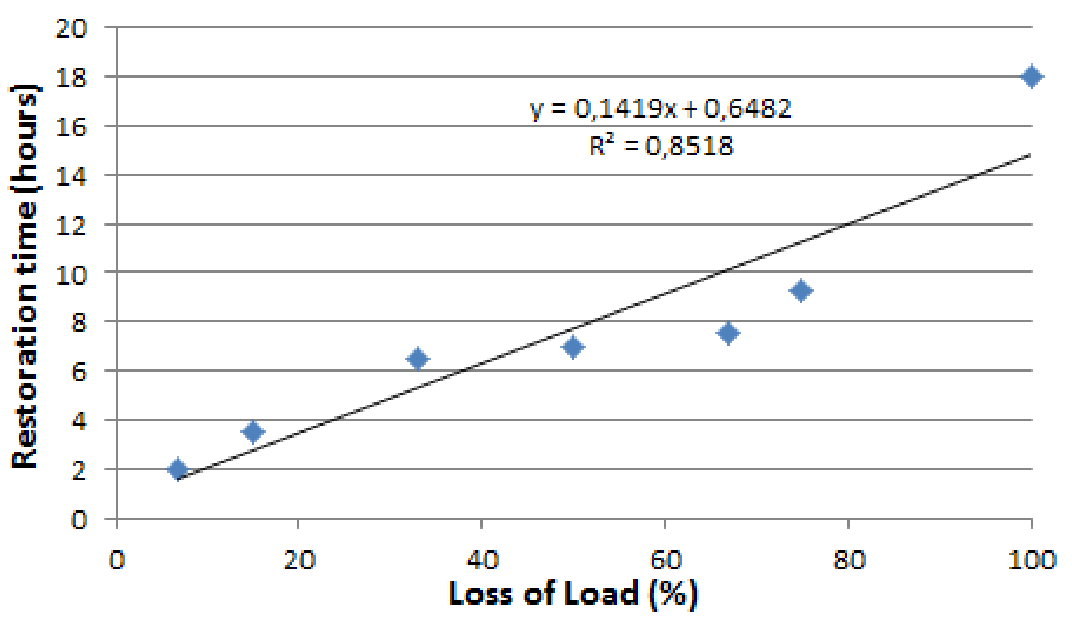
\includegraphics[width=0.6\linewidth]{Figs/RestorationTime.png}
    \caption{Restoration time of historical blackouts depending on their size~\cite{TwoLevelPSA}}
    \label{fig:restoration_time}
\end{figure}

The value of loss load is defined as the monetary value that an average consumer places on a kWh of energy not served without notice. Table~\ref{tab:VOLL} shows how this value depends on the duration of the interruption~\cite{VOLL}. It should be noted that the cost of energy not served is much larger than the cost of energy. Indeed, Table~\ref{tab:VOLL} gives values of the order of 20,000€/MWh while the price of electricity on the bulk energy market is of the order of 50€/MWh. Another simple way of estimating the value of loss load that is to consider that a one-day blackout of a country costs a 365th of its gross domestic product.

\begin{table}
    \centering
    \caption{Value of loss load, adapted from~\cite{VOLL}}
    \label{tab:VOLL}
    \begin{tabular}{@{}ll@{}}
    \toprule
    Interruption duration & Value of the loss of load \\ \midrule
    1 min  & 571 €/kWh \\
    20 min & 61 €/kWh \\
    1h     & 39 €/kWh \\
    4h     & 30 €/kWh \\
    8h     & 27 €/kWh \\
    24h    & 13 €/kWh \\ \bottomrule
    \end{tabular}
\end{table}

Based on the above reenergising model and value of loss load, the following relation can be derived between the percentage of load disconnected after a cascade and the cost for society.

\begin{equation}
    \label{eq:VOLL}
    C = \frac{3}{H} \int_0^H t \; e^{\frac{-3t}{H}} LOL \; VoLL(t) \; dt
\end{equation}
\noindent where \(H\) is the total restoration time of the blackout (estimated from Figure~\ref{fig:restoration_time}), \(LOL\) is the percentage of deenergised load at the start of the restoration process (thus \(e^{\frac{-3t}{H}} LOL\) is the percentage of deenergised load \(t\) hours after the start of the restoration), and \(VoLL\) is the value of loss load (from Table~\ref{tab:VOLL}).


\section{Conclusion}
\label{sec:security-conclusions}

This chapter has introduced the concept of power system security and the causes that can lead to a lack of security. It then presented the currently-used \emph{deterministic} methods for power system security assessment, discussed their limitations and justified the need for \emph{probabilistic} methods. Probabilistic approaches are more powerful than deterministic ones, but this comes at the cost of added complexity. In particular,

\begin{itemize}
    \item Probabilistic methods consider high-order contingencies that are neglected in deterministic assessments. They thus require to model the causes of these high-order contingencies and to estimate their frequency of occurrence.
    \item Probabilistic methods perform the security assessment on a large set of possible system states instead of on a few representative ones. This requires to generate many likely system states and to estimate their respective probability while accounting for spatio-temporal correlations between renewable energy availability at different point in the network, load, etc.
    \item Probabilistic methods quantify the potential consequences of contingencies in terms of energy not served or costs for society while deterministic methods limit the analysis to a dichotomous approach (the contingency is secure or not). They thus put higher priority on contingencies that lead to complete blackouts compared to the ones that simply lead to minor consequences. However, quantifying the consequences of a contingency requires simulating the propagation of cascading outages which is very challenging.
\end{itemize}

As discussed in section~\ref{sec:contingencies}, a large share of high-order contingencies (and resulting historical blackouts) are caused by (hidden) failures of protection systems. The modelling of protection systems and their failure modes is thus tackled in chapter~\ref{ch:protections}.

The second challenge tackled in this thesis is the simulation of cascading outages. As discussed in section~\ref{sec:cascading}, two main types of methods have been developed for the simulation of cascading outages: quasi-steady-state simulation and time-domain simulation. However, there is still no consensus on how to model ``race conditions'' between different cascading mechanisms in static simulations, and their relevance is decreasing as a growing share of cascading outages are purely driven by fast stability phenomena that can only be adequately modelled using time-domain simulations~\cite{cascadeAcceleration}.

Even when using time-domain simulations, simulating cascading outages stays a challenge as (i) it requires to simulate the system in very degraded conditions, and (ii) the evolution of a cascade might be very sensitive to modelling uncertainties because small changes in the timing protection system operations can vastly change the cascading path. Protection systems are typically not modelled in deterministic security assessments because they only operate in degraded states. However, they are a key driver in the evolution of cascading outages and are thus discussed in chapter~\ref{ch:protections}. The high sensitivity of cascading outages to protection system behaviour is also discussed in that chapter. % Chapter~\ref{ch:SPS} then focuses on system integrity protection schemes, a particular kind of protection system that can be used to increase system security.

Another important driver of cascading outages that is usually not very well modelled in deterministic assessment is the behaviour of distribution systems. Indeed, with the increasing share of distributed energy sources (rooftop solar, small- and medium-sized wind farms), distribution systems are playing a more and more active role in the stability of power systems. However, distributed energy sources tend to disconnect themselves during system disturbances, further weakening the system at the worst possible time. The modelling of distribution systems and their impact on transmission system stability is thus discussed in chapter~\ref{ch:distrib}.

Finally, because probabilistic methods consider many scenarios (combinations of possible initial system states and contingencies), and because time-domain simulations of individual scenarios are computationally expensive, it is necessary to limit as much as possible the number of simulated scenarios to be able to perform the analysis with reasonable computational resources. But of course, this should not jeopardise accuracy. Chapter~\ref{ch:DPSA} propose some methods to tackle this issue. Also, it discusses what can be done with the results a probabilistic security assessment.

\chapter{Power system protection}
\label{ch:protections}
\minitoc

\TODO{TODO}
\begin{itemize}
    \item Add figure of electrical variable evolutions for Fig.~\ref{fig:IEEE_split} and section~\ref{sec:causesOfInaccuracy}
\end{itemize}
\TODO{END TODO}

As mentioned in the previous chapters, protection systems play a key role in the triggering and the evolution of cascading outages. Indeed, failure of a protection system to clear a fault can transform a mild N-1 contingency into a more severe N-k contingency. Also, protection systems are an important driver in the development of cascading outages: trip of lines due to overloads or voltage swings, disconnection of generators, etc. Adequately modelling protection systems is thus a strong requirement to the simulation of cascading outages and therefore necessary to perform probabilistic security assessments.

This chapter starts with a brief introduction to the field of power system protections (section~\ref{sec:protection_basics}). Then, section~\ref{sec:FMEA} discusses the additional modelling requirements for protection systems in a probabilistic security assessment compared to a deterministic one.

During cascading outages, many protection systems might trip in a short amount of time (see for example the case of the 2003 US blackout illustrated in Figure~\ref{fig:BlackoutUS2003} where 200 elements were disconnected within 2 minutes). This means that small variations in the timing of protection system operations can affect the order in which elements are tripped and might therefore strongly affect the cascade propagation. Section~\ref{sec:protection_uncertainty} discuss how to handle this high sensitivity in the simulation of cascading outages.

The final section of this chapter concludes with a summary and perspectives for future work.


\section{Power system protection basics}
\label{sec:protection_basics}

The primary objective of power system protections is to protect individual assets (lines, transformers, generators) from damage that would be caused by faults or overloads by quickly disconnecting the protected elements when faults or abnormal conditions are detected. By doing so, they also affect system security, although this is a secondary objective. This section briefly introduces the basics of power system protection. It is strongly based on the ``Power System Relaying'' reference book~\cite{HorowitzBook}, and more details can thus be found in this book.

Protections systems usually consist of three main elements.

\begin{itemize}
    \item Transducers (i.e. voltage transformers (VTs) and current transformers (CTs)) that reduce the magnitude of electrical quantities to values that are easier to work with (e.g. voltages from 400~kV to 110~V and currents from 1000~A to 1~A.).
    \item A relay that measures those electrical quantities and applies some predetermined logics to decide when to trip.
    \item A circuit breaker (CB) that disconnects the protected element. Note that for elements connected to more than one terminal (e.g. lines), a protection system (including transducers, a relay and a circuit breaker) is often placed at each terminal.
\end{itemize}

The design of protection systems aims to maximise two very important objectives: dependability and selectivity. The dependability of a protection system is the likelihood that this protection will always disconnect the protected element when needed (i.e. whenever the element is faulted or subject to abnormal conditions). The selectivity of a protection system is its ability to not trip for faults for which it is not designed to operate. For example, if a line is short-circuited (e.g. following a lightning strike), this will create high currents in all nearby lines, however only the faulted line should be disconnected from the network.

Most protection systems are designed for high-dependability. This is because allowing sustained (e.g. short-circuit) faults can cause important physical damage and even deaths. On the other hand, a spurious trip (i.e. when a protection incorrectly trips during normal operation) should have no consequences in an N-1 secure system. Selectivity issues can however threaten the system stability when they occur following a fault or during a cascading outage as the system will already be weakened. Balancing dependability and security is the most challenging aspect of protection system design.

\subsection{Most common protection schemes}

The most common protection schemes are listed below. Other schemes of course exist and are presented in the reference book~\cite{HorowitzBook}.

\begin{itemize}
    \item Line protection: The most common reason why overhead transmission lines must be disconnected is the occurrence of short-circuits caused by lightning strikes falling on the line or on one of its supporting towers. Short-circuits can also be caused due to contact of the line with vegetation, or loss of a tower. Lines can also need to be disconnected due to overloads. Faulted lines need to be disconnected quickly (in the order of 100ms) to protect the line but mainly to avoid transient stability issues, but overloaded lines can generally stay connected for a few seconds to several minutes depending on the severity of the overload. The main types of line protections are given below
    \begin{itemize}
        \item Distance protection: the working principle of distance protections is shown in Figure~\ref{fig:distanceFigure}. It is based on the fact that during a metallic short-circuit of a line, the ratio between the voltage and the current (called apparent impedance) measured by the relay is equal to the impedance of the portion of the line between the relay and the fault. If this measured impedance is smaller than the impedance of the entire line, it means that the fault is on the line and that the relay should open the line. In practice, uncertainties (infeed from the other side of a resistive fault, variation of line parameters due to variable sag, etc.) imply that the presence of a fault can only be guaranteed when the apparent impedance is lower than 80 to 90\% of the line impedance. To guarantee the selectivity of the distance protection scheme, the protection is usually implemented through the use of multiple ``zones''. A common scheme is to have a ``zone 1'' that trips instantaneously when the apparent impedance is smaller than 80-90\% of the line impedance (because it is sure that the fault is actually on the line). A zone 2 trips at 110-120\% of the line impedance but with some time delay (e.g. 300ms) to allow for the protection systems of adjacent lines to trip first if the fault is not on the protected line. Using telecommunications, it is possible to have instantaneous operation for the full line. Additionally, a zone 3 is often used as a backup protection for the adjacent line(s). It thus covers the full line plus the longest adjacent line plus some margin. It operates with a larger time delay than zone 2 (e.g. 600~ms to 2~s). Distance protection is the main protection in transmission systems.
        \begin{figure}
            \centering
            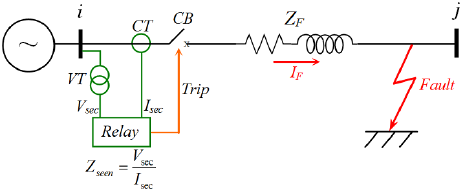
\includegraphics[width = 0.8\textwidth]{Figs/Distance.png}
            \caption{Basic schematic of distance protection~\cite{distanceFigure}}
            \label{fig:distanceFigure}
        \end{figure}
        \item Differential protection: the working principle of differential protection is that the sum of ingoing and outgoing currents in a given protected zone should be equal to zero according to Kirchhoff's law. A sum that is (significantly) different from zero indicates the presence of a fault and the necessity to trip. Due to the geographical expansions of line (dozens to hundreds of kilometres), it is necessary to have communication between both ends of a line to use differential protections. The advantage of differential protection is its high robustness and selectivity. However, it cannot act as a backup for faults outside the protected zone. It is mainly used in conjunction with distance protections for extra-high-voltage lines (400~kV in Europe) where the reliability requirements are the highest.
        \item Overcurrent protection: as the name indicates overcurrent protection disconnect the protected line when it is subject to high currents. It can either be definite-time (trips when the current is higher than a threshold for a given duration) or inverse-time (trips faster for more severe overcurrents). In transmission systems, line overcurrent protection is mostly used as (primary or backup) protection for ground faults, but distance protection is becoming more common for this application. It is also used as primary protection in some subtransmission systems and in many distribution systems~\cite{Vernova_overcurrent}.
    \end{itemize}
    \item Transformer protection: as for lines, transformers may need to be disconnected due to either internal faults or due to abnormal conditions imposed by the rest of the system. Internal faults are however rarer as transformers are less subject to external disturbances (lightning, wind). Different schemes are used to protect against internal faults and abnormal conditions:
    \begin{itemize}
        \item Internal faults: this is mainly done via differential protection thanks to its robustness and the relatively small size of transformers (a few meters vs. kilometres for lines). Other protection schemes not based on electrical variables (e.g. pressure) can also be used and are described in the reference book~\cite{HorowitzBook}.
        \item Abnormal conditions: transformers are much more sensitive too overloads than lines (overloaded lines sag, overloaded transformers lose lifespan or explode). This means that, as opposed to lines, overload protection plays an important role in transformer protection.
    \end{itemize}
    \item Generator protection: similarly to transformers, generators have to be protected against both internal faults and abnormal conditions. For electrical faults, differential protection is often used, but depending on the generator technology, many types of protection schemes can be used. Regarding abnormal conditions, the main causes of generator disconnections are listed below. It is important to note that grid codes define what are ``abnormal conditions'', i.e. define when generators should stay connected to the grid, when they are allowed to disconnect, and in some cases require them to disconnect.
    \begin{itemize}
        \item Abnormal frequency: over-frequency can cause mechanical damage in synchronous generators and their turbine; and under-frequency leads to reduce ventilation and can cause mechanical resonance. In continental Europe, generators might be quickly disconnected when frequency falls out of the 47.5-51.5~Hz range~\cite{ENTSOEgeneratorRequirements}.
        \item Low voltages: low voltage mostly affect generator auxiliary systems and indirectly affect the performance of generators. In continental Europe, generators should withstand voltage down to 0.85pu for at least 60~min~\cite{ENTSOEgeneratorRequirements}.
        \item Fault ride-through: generators should be able to stay connected when temporary faults occur in their vicinity (e.g. lightning strike on a nearby line). Ride-through requirements are defined using curves as in Figure~\ref{fig:LVRT_G99}. As long as the generator voltage stays above the curve following a disturbance, the generator must stay connected. If voltage falls below the curve (e.g. if the voltage is lower than 0.7pu more than 140ms after the occurrence of the fault), the generator is allowed to disconnect.
        \begin{figure}
            \centering
            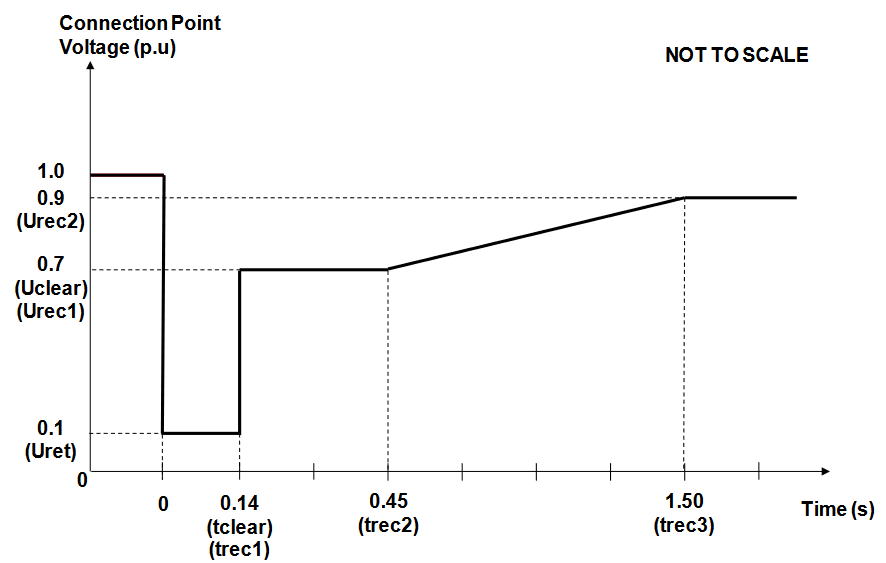
\includegraphics[width = 0.6\textwidth]{Figs/LVRT.png}
            \caption{Fault ride-through profile for large synchronous generators in the UK~\cite{G99}}
            \label{fig:LVRT_G99}
        \end{figure}
        \item Overexcitation: when a synchronous generator simultaneously produces high active and reactive power, it leads to high stator currents that can overheat the generator. When this occurs, the generator excitation will automatically be reduced after a few minutes to reduce the reactive power production and protect the generator. However, this can cause long-term voltage stability issues.
    \end{itemize}
    \item System protection: some protection systems do not aim to protect a particular element of the grid, but to protect the stability of the grid itself. Some key examples are listed below.
    \begin{itemize}
        \item Under-frequency load shedding (UFLS): UFLS relays are a last-resort solution to severe load generation imbalances following large generator disconnections or system splits. In Europe, UFLS relays disconnect load by steps when frequency falls between 49 and 48~Hz (increasingly more steps are activated the lower the frequency falls)~\cite{ENTSOE-UFLS}.
        \item Out-of-step relaying: power system swings can cause distance relays to operate. Indeed, let's consider that during a swing of the 2-generator system shown in Figure~\ref{fig:OOS}, the two generator angles are 180° from each other (the maximum value for a stable swing according to the basic equal area criterion), and that the voltage magnitude at the two generators are approximately equal. Then, these two voltages will cancel out for point that are at an equal electrical distance from the two generators. Points with zero or low voltage will be seen at faults by distance relays. These relays might then trip if they see an apparent impedance that stays in one of their zone of operation for more than the zone time delay. Out-of-step relays can distinguish faults from power swings thanks to their different timescales (faults occur in a few milliseconds, swings in hundreds of milliseconds) and can be used to block the operation of distance relays. During unstable swings, they can split the system at predefined locations with the aim of creating balanced islands. For example, the split shown in Figure~\ref{fig:OOS} would be beneficial if the active output of generator \(G_1\) is close to the sum of loads \(L_2\) and \(L_4\), and the output of \(G_3\) close to the load of \(L_5\).
        \begin{figure}
            \centering
            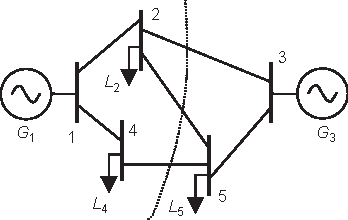
\includegraphics[width = 0.5\textwidth]{Figs/Out_of_step.pdf}
            \caption{System separation by out-of-step relays~\cite{HorowitzBook}}
            \label{fig:OOS}
        \end{figure}
        \item Other system integrity protection schemes (SIPSs)~\cite{IEEE_SIPS, CIGRE_SIPS_tutorial}: the push to operate power grids closer to their limits has led to an increasing popularity of SIPSs. SIPS are ``designed to detect abnormal system conditions and take predetermined, corrective action (other than the isolation of faulted elements) to preserve system integrity''. SIPSs can be designed to solve a wide variety of issues, and as such there are many existing SIPS designs. SIPSs can either be event-based (respond to an event, e.g. loss of a line) or response-based (respond on a system condition, e.g. loss of synchronism), and they can be either centralised (gather all needed information to a central location (e.g. the control centre) and send control signals using telecommunications) or decentralised. They are increasingly being used as part of defence plans of TSOs~\cite{CigreDefensePlan, ENTSOEdefencePlan}.
    \end{itemize}
\end{itemize}



\section{Modelling protection systems in probabilistic security assessments}
\label{sec:FMEA}

Because deterministic security assessments usually do not consider N-k contingencies nor cascading outages, they generally model protection systems in a very simplified manner. For example, for a line fault, it is generally assumed the fault will be cleared in normal time (or in backup clearing time to have a margin) by opening the line. And since no cascading outage should occur, it is assumed that no other protection system will operate.

In probabilistic assessments however, the possibility of a failure to normally clear the fault is considered. Such protection failures can lead to N-k contingencies as adjacent branches need to be disconnected to clear the fault. The impact and reasons for protection systems failing to normally clear faults is discussed in section~\ref{sec:protection_clearing}.

As cascading outages need to be simulated in probabilistic assessments, it is also important to consider the impact of protection systems beyond the clearing of the initial fault. Indeed, protection systems play a key role in the propagation of cascading outages and thus need to be modelled adequately. This is discussed in section~\ref{sec:protection_cascade}.


\subsection{Impact of protection systems after an initial fault}
\label{sec:protection_clearing}

To understand the impact and estimate the probability of protection failure to clear a fault, it is important to note that, as for any critical system, multiple layers of redundancy are used to make sure that faults are cleared in a timely manner and with minimum impact on the system. This is especially true at higher voltage levels where higher levels of redundancy are used.

Figure~\ref{fig:fault_clearing} demonstrates this with an example. In this example, there is a fault on line AB. Normally, the relays R\textsubscript{1} and R\textsubscript{5} located at both ends of the line will see this fault and respectively send tripping signals to the breakers B\textsubscript{1} and B\textsubscript{5}. This is the primary protection of line AB, and it clears the fault simply by opening both ends of the line as shown in Figure~\ref{subfig:clearing_normal}.

\begin{figure}
    \centering
    \subfloat[Clearing of the fault F by the primary protection (R\textsubscript{1} or its duplicate R\textsubscript{2}), typical clearing time: 100ms]{%
        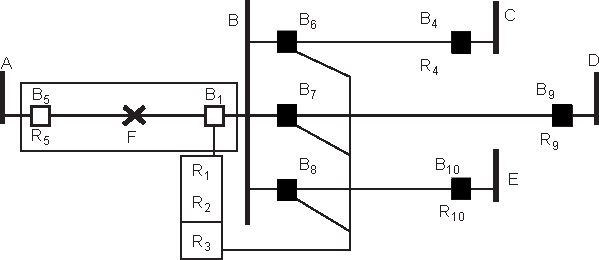
\includegraphics[width=0.7\linewidth]{Figs/Clearing_normal.pdf}
        \label{subfig:clearing_normal}
    } \\ \vskip 0.5 \baselineskip
    \subfloat[Use of local backup protection following failure to open of breaker B\textsubscript{1}, typical clearing time: 200ms]{%
        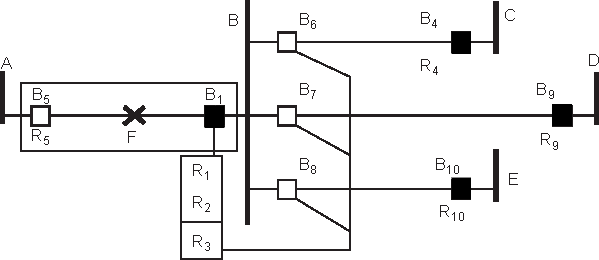
\includegraphics[width=0.7\linewidth]{Figs/Clearing_breaker.pdf}
        \label{subfig:clearing_breaker}
    } \\ \vskip 0.5 \baselineskip
    \subfloat[Fault clearing by remote backup, typical clearing time: 500ms-2s]{%
    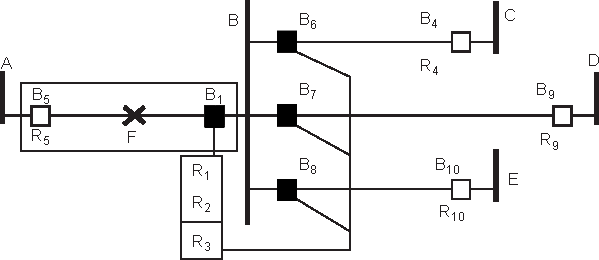
\includegraphics[width=0.7\linewidth]{Figs/Clearing_Z3.pdf}
    \label{subfig:clearing_Z3}
    }
    \caption{Duplicate primary, local backup, and remote backup protection, based on~\cite{HorowitzBook}. Black breakers are closed, white breakers are open.}
    \label{fig:fault_clearing}
\end{figure}

To increase the dependability of this scheme, elements of the primary protection can be duplicated. In this example, R\textsubscript{2} acts as a duplicate for R\textsubscript{1}. The duplicate can be identical to R\textsubscript{1} or use a different protection scheme (e.g. use of both differential and distance protection). The transducers and battery power supply can also be duplicated. The breaker is usually not duplicated due to its higher cost.

R\textsubscript{3} acts as a local backup, also called breaker failure protection. If R\textsubscript{1} or R\textsubscript{2} sends a tripping signal but B\textsubscript{1} does not open, R\textsubscript{3} will send a trip signal to B\textsubscript{6}, B\textsubscript{7} and B\textsubscript{8} as shown in Figure~\ref{subfig:clearing_breaker}. This allows for the fault clearing despite failure of breaker B\textsubscript{1} but requires the disconnection of non-faulted elements (lines BC, BD, and BE) leading to an N-4 contingency in this case. Also, breaker failure protection operates with a larger time delay than the primary protection which challenges dynamic stability.

If either

\begin{itemize}
    \item Both R\textsubscript{1} and R\textsubscript{2} fail to see the fault (and thus send no signal to B\textsubscript{1} nor to the breaker failure protection relay R\textsubscript{3})
    \item R\textsubscript{1} or R\textsubscript{2} operate, but B\textsubscript{1} fails to open and breaker failure protection (R\textsubscript{3}) fails
    \item R\textsubscript{1} or R\textsubscript{2} operate, but B\textsubscript{1} fails to open and no breaker failure protection schemes is installed
\end{itemize}
\noindent then, the remote backup protection of relays R\textsubscript{4}, R\textsubscript{9} and R\textsubscript{10} will need to be activated as shown in Figure~\ref{subfig:clearing_Z3}. This remote backup protection is often performed by zone 3 relays and thus needs even more time to clear the fault than primary or local backup protection.

The example above considered that substations each consist of a single bus single that directly connects all incident lines together, so that breaker failure protection need to open all breakers in a substation. However, different types of substation configurations can be used to reduce the impact of breaker failure (and to increase reliability in general). Figure~\ref{fig:substation} shows the most common substation configurations and how they are impacted by breaker failure.

Figure~\ref{subfig:substation_single} shows the single-bus, single-breaker substation discussed in the previous example. The substation is made of a single bus and all elements are connected to this bus through a single-breaker. This is the simplest configuration, however, if a fault occurs on one of the elements and the associated breaker fails to open, all other breakers need to open in order to isolate the fault.

At the other end of the reliability spectrum lies the two-bus, two-breaker substation configuration (Figure~\ref{subfig:substation_double}). This substation consists of two buses, and each element is connected to each bus via a breaker (so, two breakers are needed per element, hence the name). When a fault occurs on one of the elements, both its breakers need to be opened. If one breaker fails to open, all other breakers connected to the same bus will need to open to isolate the fault. However, as (non-faulted) lines are still connected to the other bus, they remain in service. In this configuration, failure of a (single) breaker does not cause the loss of additional elements. However, it requires twice as many breakers per connected elements than the previous case, so it is basically twice as expensive.

\begin{figure}
    \centering
    \subfloat[Single-bus, single-breaker substation: all lines are disconnected following breaker failure to open]{%
        \begin{minipage}{0.45\linewidth}
            \centering
            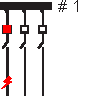
\includegraphics[height=0.15\textheight]{Figs/BFP_single_bus.pdf}
        \end{minipage}
        \label{subfig:substation_single}
    } \hfill
    \subfloat[Two-bus, two-breaker substation: bus 2 is disconnected, but all (non-faulted) lines remain connected]{%
        \begin{minipage}{0.45\linewidth}
            \centering
        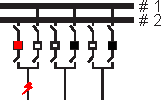
\includegraphics[height=0.15\textheight]{Figs/BFP_double_breaker.pdf}
        \end{minipage}
        \label{subfig:substation_double}
    } \\ \vskip 2 \baselineskip
    \subfloat[Two-bus, single-breaker substation: lines that are connected to the same bus as the faulted line are lost (here, it is assumed that lines 1 and 3 are initially connected to bus 1, and lines 2 and 4 to bus 2)]{%
        \begin{minipage}{0.45\linewidth}
            \centering
        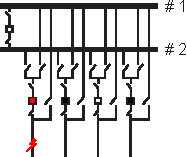
\includegraphics[height=0.2\textheight]{Figs/BFP_two_bus_one_breaker.pdf}
        \end{minipage}
        \label{subfig:substation_two_bus_one_breaker}
    } \hfill
    \subfloat[Ring substation: the bottom right line is lost due to breaker failure]{%
        \begin{minipage}{0.45\linewidth}
            \centering
        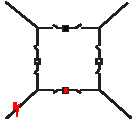
\includegraphics[height=0.2\textheight]{Figs/BFP_ring.pdf}
        \end{minipage}
    \label{subfig:substation_ring}
    } \\ \vskip 2 \baselineskip
    \subfloat[Breaker-and-a-half substation: one line is lost for failure to open of the middle breaker]{%
        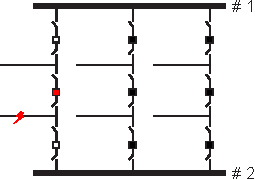
\includegraphics[width=0.45\linewidth]{Figs/BFP_half_middle.pdf}
    \label{subfig:substation_half_middle}
    } \hfill
    \subfloat[Breaker-and-a-half substation: bus 2 is disconnected, but all lines remain connected]{%
        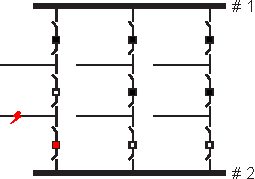
\includegraphics[width=0.45\linewidth]{Figs/BFP_half_bottom.pdf}
    \label{subfig:substation_half_bottom}
    }
    \caption{Impact of breaker failure to open in different substation configurations, based on~\cite{HorowitzBook}. All breakers are assumed initially closed in this example. Black breakers are closed, white breakers are open, and red breakers are stuck close.}
    \label{fig:substation}
\end{figure}

Figure~\ref{subfig:substation_two_bus_one_breaker} shows a two-bus, single-breaker substation. This configuration consists of two buses, but each element is normally only connected to one of the two buses (switches can change to which bus an element is connected but only when the element is not energised). A breaker connects the two buses such that all elements are connected together\footnote{The busbar coupler can be opened even without the presence of a fault in order to split the substation and change the power flows in and around the substation.}. In case of breaker failure, the breaker that connects the two buses is opened such that only elements that are connected to the same bus as the faulted element need to be disconnected. In this example (Figure~\ref{subfig:substation_two_bus_one_breaker}), breaker failure leads to N-2 contingencies, while it would have led to N-4 contingencies with the single-bus configuration.

Ring substations (Figure~\ref{subfig:substation_ring}) consist of a ring of circuit-breakers with one element connected between each pair of breakers. In this configuration, a faulted element requires two breakers to open, but breaker failure only causes the loss of one additional element.

Breaker-and-a-half substations (figures~\ref{subfig:substation_half_middle} and~\ref{subfig:substation_half_bottom}) consist of two buses linked by chains made of three breakers in series. One element is connected between the first and second, and between the second and third breaker of each chain. This configuration is called breaker-and-a-half because, on average, it requires one and a half breaker per connected element (in this example, 9 breakers for 6 elements). As shown in the figures, failure to open the middle breaker leads to the loss of one additional element, and failure to open the first or third breaker does not cause the loss of any additional element.

Modelling the possible failures of protection systems as discussed above can be done using standard reliability analysis techniques. Ref.~\cite{GridPSA, Haarla} provide many examples of event trees that describe the impact of protection failure on fault clearing. They also use fault trees to estimate the probability of the possible outcomes of a fault (normal clearing, delayed clearing, clearing with breaker failure protection, etc.) based on fault statistics of protection elements (relays, breakers, transducers, etc.) gathered in Finland and the other Nordic countries.

The discussion above has focused purely on protection system failure to clear faults, i.e. on the lack of dependability of protection systems. Another issue of protection systems is that they do not have 100\% selectivity, i.e. they will sometimes cause unnecessary trips. Unwanted trips that occur ``spontaneously'', i.e. without the occurrence of a fault, pose low risk to system security as they simply cause N-1 contingencies against which the system should normally be secure. However, unwanted trips that occur as a consequence of a fault will lead to N-2 contingencies (one element lost because it is faulted, the second because of the unwanted trip) that pose higher risks.

Modelling of unwanted trips is a complex issue. Historically, there has been much emphasis on the possibility of relays to trip due to misoperation of zone 3 distance protection caused by a timer stuck close~\cite{ZoneVulnerability, OriginalManchesterModel}. Indeed, in legacy electromechanical relays, the time-delay of zone 3 was implemented by a physical timer that could get stuck causing the zone 3 to operate without time delay. This failure mode no longer exist in numerical relays, but up until very recently, there has been little updates in the unwanted tripping models of distance relays~\cite{Alexandre_PMAPS}. Another issue caused by zone 3 was the tendency of relays to trip in high loading conditions (high loads are seen as small impedances)~\cite{3rdZoneRevisited} as seen in the US 2003 blackout. This issue has also been made less prevalent by numerical relays that can use load blinders to distinguish between remote faults and high-load conditions.

A major cause of protection misoperations is the inadvertent use of wrong settings in protection relays (this issue is actually made worse with modern relays) and design errors~\cite{ProtectionMisoperationsBian2012}. These issues are extremely difficult to model and no unwanted tripping model for modern numerical relays could be found in the literature. Unfortunately, due to lack of time, no model is proposed in this thesis either.

\begin{tcolorbox}[width=\linewidth, %sharp corners=all,
    colback=red!5!white,
    colframe=red!75!black,
    breakable,
    title=Note]
One key highlight of~\cite{GridPSA} is that, when using historical failure statistics, one should pay attention to the kind of failures that are reported. For example, ref.~\cite{GridPSA} estimates SF6 circuit breaker failure rates based on Finnish statistics (0.0028 failures to open, and 0.01 failures to reclose per year, for a total of 0.0128 failures per year) and compare it to the value published in a CIGRE report (0.012 failures per year). The two failure rate estimates are very close. However, ref.~\cite{GridPSA} distinguishes between failure to open and failure to reclose because failures to open pose a significantly greater security risk (transform N-1 contingencies into N-k ones as discussed above).

Similarly, ref.~\cite{GridPSA} reads from a report that most unwanted Finnish trips are spontaneous at the highest voltages (400 and 220~kV) and unselective at 110~kV. However, they did not have figures for unselective trips at high voltage levels which are the most critical for system security. In conclusion, careful attention should be paid to what are the failure modes considered in fault statistic reports and at what voltage levels they occurred.
\end{tcolorbox}



\subsection{Impact of protection systems during cascading outages}
\label{sec:protection_cascade}

Protection systems play a key role in the development of cascading outages. It is thus necessary to model them explicitly in the power system simulator used to study the cascading outages. All time-domain cascading simulators in the literature model the expected behaviour of the most common types of protection systems. For example, for distance relays, the associated model would compute the apparent impedance seen by the relays and would trip if this impedance stays in a protected zone for longer than its time-delay as shown in algorithm~\ref{alg:distance} (simplified for the sake of brevity). % The protection system models developed in this thesis are available online\footnote{\url{https://github.com/dynawo/dynawo/tree/master/dynawo/sources/Models/Modelica/Dynawo/Electrical/Controls/Protections}}.

\begin{algorithm}
\centering
\caption{Simplified distance protection model with a single protected zone}\label{alg:distance}
\begin{algorithmic}[1]
\State \(t_{Breaker} \gets\) 80ms
\State \(t_{ZoneDelay} \gets\) 300ms (typical value for zone 2, other values should be used for different zones)
\State \(\underline{Z} \gets \dfrac{\underline{U}}{\underline{I}}\)

\\
\If{\(\underline{Z}\) is in the protected zone and \(t_{Arming} = \infty\)}
    \State \(t_{Arming} \gets t\)
\ElsIf{\(\underline{Z}\) is outside the protected zone}
    \State \(t_{Arming} \gets \infty\)
\EndIf

\\
\If{\(t > t_{Arming} + t_{ZoneDelay}\)}
    \State \(t_{Trip} \gets t\)
\EndIf

\\
\If{\(t > t_{Trip} + t_{Breaker}\)}
    \State Disconnect protected element
\EndIf

\end{algorithmic}
\end{algorithm}

Multiple types of protection systems can operate during cascading outages and should thus be adequately modelled. Based on historical disturbances, ENTSO-E listed the types of protections most likely to operate during cascading outages~\cite{ENTSOEdefencePlan}:

\begin{itemize}
    \item Distance protection (first and higher zones)
    \item Overcurrent relays
    \item Differential relays
    \item Under-frequency load shedding
    \item Under-voltage load shedding
    \item Generator protection
    \begin{itemize}
        \item Under- and over-voltage relays
        \item Under- and over-frequency relays
        \item Loss-of-field relays
        \item Volt/Hz over-excitation relays
        \item Generator backup relays
    \end{itemize}
\end{itemize}

Moreover, as discussed above, there are three additional complexities that can be considered in the modelling of protection systems:

\begin{itemize}
    \item Missing trips: protection systems might not trip when expected to either due to a failure of an element of the protection system (relay, breaker), or due to a misoperation of the relay.
    \item Unwanted trips: relays might send tripping signals when not expected to.
    \item Sensitivity of cascading outages to small changes in protection behaviour: small changes in the timing of protection systems operation can impact the order in which protection systems operate, and potentially vastly impact the cascade evolution.
\end{itemize}

Missing trips caused by relay or breaker failures can relatively easily be modelled as has been done in the DCAT tool~\cite{DCATphase1} and in approaches based on dynamic event trees~\cite{TwoLevelPSA}. In DCAT, when a protection system operates during a cascade, two possible branches of the simulation are created: one where the protection actually operates and one where it fails to. The frequency associated with each branch is weighted according to the probability of the protection system to operate (for the former branch) or to fail (for the latter)\footnote{As protection systems are often designed to protected individual elements and not the grid itself, it can be argued that, once a cascade is initiated, protection failures might not necessarily negatively impact system stability. And, since protection failures are unlikely, their contribution to the risk might be negligible. Indeed, chapter~\ref{ch:DPSA} demonstrates that for the considered test system, protection failures to operate during cascading outages do not significantly impact the risk estimate. However, this might be system dependent and the argument is of course not valid for SIPSs.}. This probability can be estimated based on standard reliability techniques (e.g. fault trees).

During cascading outages, power system operate in very degraded states which can cause protection system misoperations leading to both missing and unwanted trips. The most common misoperations have been reported by the IEEE Power System Relaying and Control Committee (PSRC)~\cite{ProtectionFailuresDemetrios, PSRCreportProtectionMisop, PSRCreportSummaryProtectionMisop} and are listed below.

The main contributor of relay misoperations is again (zone 3) distance protection. Indeed, distance protection can trip following power swings, high loads, and low-voltage conditions\footnote{In the case of low voltages, loads will tend to increase the current they draw, trying to partially maintain a constant power draw, and thus leading to low-voltage, high-current conditions. Such conditions are seen as small apparent impedances by distance relays that are thus likely to trip}. However, such misoperations can easily be modelled by explicitly representing the relays in a time-domain simulator (as shown in the simplified algorithm~\ref{alg:distance}). Of course, if some distance relays have load blinders and power swing blocking functionality, these should be modelled too. Similarly, although less often used on the high-voltage levels, overcurrent protections can also trigger during power swings, high-load, or low-voltage conditions.

Another issue is the operation of backup ground overcurrent relays of highly-loaded untransposed lines. Indeed, untransposed lines can have current imbalances up to 10\% creating a zero sequence component. This can be enough to trigger ground overcurrent relays in case of high loads (or transient high currents). In modern relays however, this issue can be alleviated by restraining the ground overcurrent relays by a fraction of the positive sequence current.

Frequency deviations can cause inaccuracies in the evaluation of phasors. However, as frequency should always stay within 5\% of its nominal value (otherwise the system is already on its way to a complete blackout), the associated errors are small. These errors also depends on which frequency tracking scheme is used by the relays and are thus simply modelled as measurement errors in this thesis. They are thus handled in section~\ref{sec:protection_uncertainty}.

Finally, ref.~\cite{ProtectionFailuresDemetrios, PSRCreportProtectionMisop, PSRCreportSummaryProtectionMisop} discusses issues related to the polarisation of relays (voltage angle estimated from past measurement when voltages too low for an accurate measurement). However, as these issues mainly affect legacy mho relays, they are not considered in this thesis.



\section{Handling uncertain protection behaviour in simulations of cascading outages}
\label{sec:protection_uncertainty}

\begin{tcolorbox}[width=\linewidth, sharp corners=all,
    colback=white!80!black,
    colframe=white!80!black]
This section is partly based on the following publication:
\begin{itemize}
    \item \fullcite{ISGT2023_Protections}
\end{itemize}
\end{tcolorbox}

During fast cascading outages, many protection systems can operate in a very short period of time. This renders the simulation of cascading outages quite complex as small modelling uncertainties can potentially have high impacts on which protection systems actually operate and in which order, therefore strongly affecting how the cascade propagates.

One example of such fast cascade occurred on 8 January 2021 and led to the separation of the Continental Europe power system into two synchronous regions as shown in Figure~\ref{fig:split2021}. The split occurred when there were high power flows from South-Eastern Europe to North-Western Europe and was initiated by the decoupling of two busbars in the Ernestinovo substation due to busbar coupler overload protection. (This event can be loosely classified as an N-2 event as it interrupted SE-NW flows along two axis (Ugljevik-Zerjavinec and Sremska Mitrovica-Pecs) as shown in Figure~\ref{fig:split2021_timeline}.) High power flows and the reduced transmission capacity caused by the busbar coupler trip led to angle instability and a subsequent split of the system in a cascading manner.

\begin{figure}
    \centering
    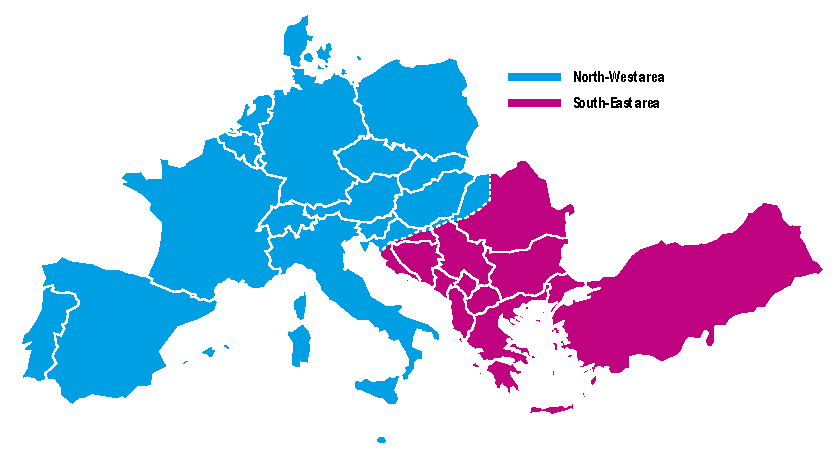
\includegraphics[width = 0.7\textwidth]{Figs/SystemSplit2021.pdf}
    \caption{Resulting two synchronous areas after the 8 January 2021 European system split~\cite{ENTSOESplitJan2021}}
    \label{fig:split2021}
\end{figure}

\begin{figure}
    \centering
    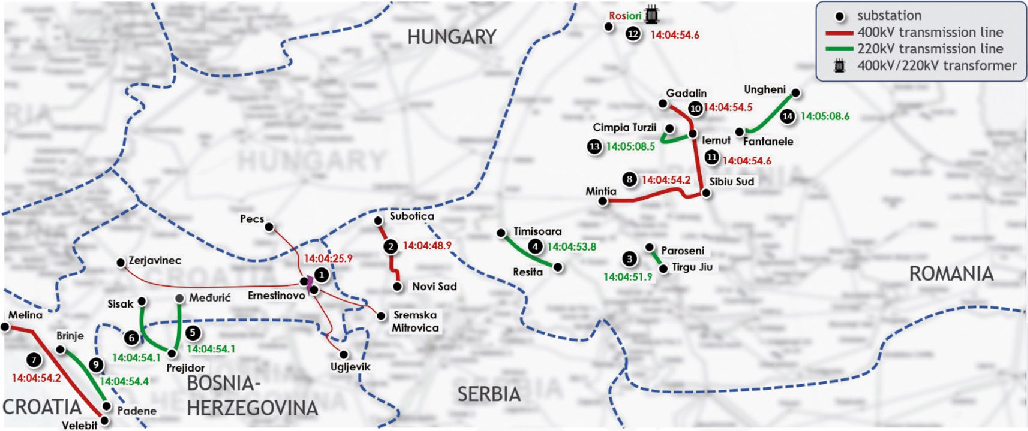
\includegraphics[width = \textwidth]{Figs/SystemSplitTimeline2021.pdf}
    \caption{Geographical location of elements tripped during the 8 January 2021 European system split~\cite{ENTSOESplitJan2021}. Trip of 110~kV lines are not represented.}
    \label{fig:split2021_timeline}
\end{figure}

\begin{table}
\centering
\caption{Timeline of events that led to the 8 January 2021 European system split~\cite{ENTSOESplitJan2021}. Approximately 15 110~kV lines were tripped but are not listed.}
\label{tab:split_timeline}
\begin{adjustbox}{max width=\textwidth}
\begin{tabular}{@{}lllllll@{}}
\toprule
No & Country & delta [s] & Substation 1 & Substation 2   & Voltage [kV] & Reason                                                 \\ \midrule
1a & Croatia & 0         & Ernestinovo  &                & 400          & Busbar coupler overload protection                     \\
1b & Croatia & 2.6       & Ernestinovo  &                & 400/110      & Overload protection of both 400 / 110 kV transformers  \\
2  & Serbia  & 23        & Subotica     & Novi Sad       & 400          & Overload protection 20s 2nd zone                       \\
3  & Romania & 26        & Paroșeni     & Târgu Jiu Nord & 220          & Distance protecton starting zone 2.4 s                 \\
4a & Romania & 27.9      & Reşiţa       & Timişoara      & 220          & Distance protection 0.4 s                              \\
4b & Romania & 27.9      & Reşiţa       & Timişoara      & 220          & Distance protection 0.4 s breaker L1 failure           \\
5  & Bosnia  & 28.2      & Prijedor     & Međuriċ        & 220          & Distance protection out-of-step protection             \\
6  & Bosnia  & 28.2      & Prijedor     & Sisak          & 220          & Distance protection out-of-step protection             \\
7  & Croatia & 28.3      & Melina       & Velebit        & 400          & Distance protection zone 3                             \\
8  & Romania & 28.3      & Mintia       & Sibiu          & 400          & Distance protection power swing condition              \\
9  & Croatia & 28.5      & Brinje       & Padene         & 220          & Distance protection zone 1                             \\
10 & Romania & 28.6      & Gădălin      & Iernut         & 400          & Distance protection power swing condition zone 2 0.4 s \\
11 & Romania & 28.7      & Sibiu Sud    & Iernut         & 400          & Distance protection zone 3 reverse 0.6 s               \\
12 & Romania & 28.7      & Roşiori      &                & 400/220      & Distance protection power swing condition              \\
13 & Romania & 42.6 & Iernut & Câmpia Turzii & 220 & Distance protection zone 2 power swing conditions \\
14 & Romania & 42.7      & Fântânele    & Ungheni        & 220          & Distance protection zone 2 power swing conditions      \\ \bottomrule
\end{tabular}
\end{adjustbox}
\end{table}

The trips that led to the system separation are listed in Table~\ref{tab:split_timeline} and shown in Figure~\ref{fig:split2021_timeline}. As can be seen from the table, events 4 to 12 occur in less than a second showing the possibility of different tripping orders. Also, it demonstrates the importance of distance protection in the development of cascading outages. Finally, it can be noted that some TSOs use power swing blocking for distance protection and some do not.

Similarly, although not the focus of this thesis, slow cascades are also affected by modelling uncertainties. The tripping of overloaded lines is caused by lines sagging into vegetation and thus depends on uncertain parameters as vegetation height, temperature and wind. % The order of trips can thus also be affected by uncertainties.

A common approach to handle uncertainties is to use Monte Carlo (MC) simulations and their derivatives. Notably, in~\cite{TwoLevelPSA}, fast cascading outages are simulated with dynamic event trees where each possible realisation of a protection system behaviour leads to different possible branches. In~\cite{SequencesRelaySobol}, the order of protection system operation is encoded in a matrix that is then used with extended forms of variance-based sensitivity estimators to rank how sensitive cascading outages are to different power system variables.

The issue with MC techniques is that they can be computationally expensive. This poses an important challenge for this thesis as systematic probabilistic dynamic security assessments require to simulate many cascading outage scenarios. To alleviate this challenge, a simple indicator has been developed to predict which cascading outage scenarios are sensitive to protection-related uncertainties and which are not. MC simulations then only have to be performed for the former limiting their impact of computation time. The simple indicator is presented in section~\ref{sec:protection_indicator}. It is applied on a standard test system with a set of protection systems described in section~\ref{sec:protection_test_case}, and its performance is discussed in section~\ref{sec:protection_results}.


\subsection{Identifying sensitive scenarios}
\label{sec:protection_indicator}

The objective of the indicator is to predict which scenarios (combination of a given initial system state and of a contingency) lead to cascading outages whose evolution is sensitive to protection-related uncertainties and which scenarios do not.

The indicator is constructed by building and comparing two extreme trip sequences. The first sequence is generated by simulating the system with protection systems operating as slowly as possible (leading to a so-called ``slow sequence'' of tripping events (Fig.~\ref{subfig:slowSeq})). This is done by selecting, in the distribution of the protection parameters, the values that lead to the slowest protection operations. For example, for a distance protection, this would imply taking the smallest value of the size of the zones of operation, and the largest value for the opening time of the circuit breaker. The second sequence is generated by simulating the system with fast protection systems (leading to a ``fast sequence'' of tripping events).%\footnote{Actually, it is sufficient to only accelerate the operation of distance protections when generating the faster sequence. According to our tests, accelerating only the distance protections or all protections leads to the same performance of the indicator. This can be explained by the fact that, most often, distance protections are the ones that initiate fast cascading outages~\cite{ENTSOESplitJan2021, ENTSOEIbericSplit2021}.}

\begin{figure}
    \centering
    \subfloat[Slow sequence (reference)]{%
        \begin{tikzpicture}[scale=1.5]
        % draw horizontal line
        \draw (0,0) -- (7,0);

        % draw vertical lines
        \foreach \x in {0,1,4.5,6,7}
          \draw (\x cm,3pt) -- (\x cm,-3pt);

        % draw nodes
        \draw (1,0) node[below=3pt] {$ 1_a $};
        \draw (4.5,0) node[below=3pt] {$ 2_a $};
        \draw (6,0) node[below=3pt] {$ 3_a $};
        \end{tikzpicture}
        \label{subfig:slowSeq}
        } \\ \vskip\baselineskip
    \subfloat[Fast sequence for which the system is unlikely to be affected by protection-related uncertainties]{%
        \begin{tikzpicture}[scale=1.5]
        % draw horizontal line
        \draw (0,0) -- (7,0);

        % draw vertical lines
        \foreach \x in {0,1,4,5.5,7}
          \draw (\x cm,3pt) -- (\x cm,-3pt);

        % draw nodes
        \draw (1,0) node[below=3pt] {$ 1_b $};
        \draw (4,0) node[below=3pt] {$ 2_b $};
        \draw (5.5,0) node[below=3pt] {$ 3_b $};
        \end{tikzpicture}
        \label{subfig:negative}
     } \\ \vskip\baselineskip
    \subfloat[Fast sequence likely to be affected: \(3_c\) occurs before \(2_a\)]{%
        \begin{tikzpicture}[scale=1.5]
        % draw horizontal line
        \draw (0,0) -- (7,0);

        % draw vertical lines
        \foreach \x in {0,1,2,3,7}
          \draw (\x cm,3pt) -- (\x cm,-3pt);

        % draw nodes
        \draw (1,0) node[below=3pt] {$ 1_c $};
        \draw (2,0) node[below=3pt] {$ 2_c $};
        \draw (3,0) node[below=3pt] {$ 3_c $};
        \end{tikzpicture}
        \label{subfig:order}
    } \\ \vskip\baselineskip
    \subfloat[Fast sequence likely to be affected: a new event (\(4_d\)) occurs]{%
        \begin{tikzpicture}[scale=1.5]
        % draw horizontal line
        \draw (0,0) -- (7,0);

        % draw vertical lines
        \foreach \x in {0,1,4.5,6,6.5,7}
          \draw (\x cm,3pt) -- (\x cm,-3pt);

        % draw nodes
        \draw (1,0) node[below=3pt] {$ 1_d $};
        \draw (4.5,0) node[below=3pt] {$ 2_d $};
        \draw (6,0) node[below=3pt] {$ 3_d $};
        \draw (6.5,0) node[below=3pt] {$ 4_d $};
        \end{tikzpicture}
        \label{subfig:new_event}
    }
    \label{fig:fig}
    \caption{Classification of tripping sequences according to the proposed indicator}
\end{figure}

The indicator predicts that a scenario is sensitive to uncertainties if either

\begin{itemize}
    \item Comparing the two sequences shows the possibility for two events to be swapped (Figure~\ref{subfig:order}).
    \item If one event occurs in one sequence but not in the other (Figure~\ref{subfig:new_event}).
\end{itemize}

The first condition detects cases where uncertainties can affect the order of protection system operations. And the second detects ``near-misses'', i.e. cases where one protection does not operate but is very close to (e.g. for a distance protection, the apparent impedance enters the protected zone but leaves just before the protection time delay). Regarding the first condition, it should be noted that events could occur in the same order in both the slow and fast sequences (as shown in Figures~\ref{subfig:slowSeq} and~\ref{subfig:order}) but still indicate the possibility for uncertainties to affect the order of protection system operations. Indeed, in Figure~\ref{subfig:order}, the event \(3_c\) occurs before \(2_a\) highlighting the possibility for events \(2\) and \(3\) to be swapped.

To avoid having to perform two simulations for each scenario (one with slower and one with faster protection systems), it is also possible to perform a single simulation with models of both slower and faster protections. In this case, the faster protection systems should not be connected to a circuit breaker, so that they do not affect the system evolution but still generate the log messages needed to generate the fast sequence. This is an approximation (the fast sequence is based on the system evolution with slow protection), but it has a small impact on the precision of the indicator (as shown in section~\ref{sec:protection_results}) and requires only one simulation instead of two.


\subsection{Test case and protection system models}
\label{sec:protection_test_case}

The test case used in this example is the IEEE 39-bus test system~\cite{IEEE39} shown in Figure~\ref{fig:IEEE39} with dynamic data taken from~\cite{IEEE39Dynamic} and a few minor modifications made to make the system more realistic~\cite{ISGT2023_Protections}.

\begin{figure}
    \centering
    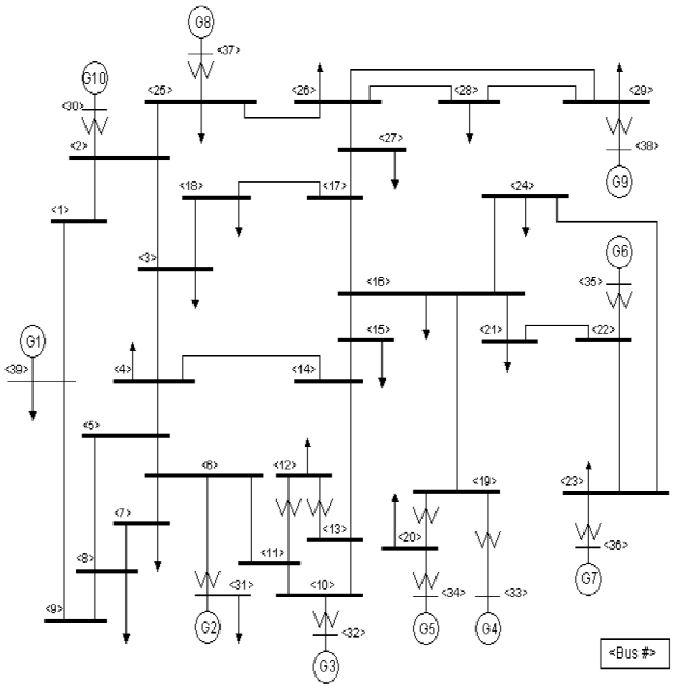
\includegraphics[width=0.7\textwidth]{Figs/IEEE39.png}
    \caption{IEEE 39 bus system~\cite{IEEE39figure}}
    \label{fig:IEEE39}
\end{figure}

The load model has been changed to a restorative exponential load model, i.e.

\begin{equation}
\label{eq:restorative_load_model_1}
P = P_0 \left(\frac{U}{U_f}\right)^2, \quad Q = Q_0 \left(\frac{U}{U_f}\right)^2
\end{equation}
\noindent where \(P\) (resp. \(P_0\)) and \(Q\) (\(Q_0\)) are the (initial) active and reactive power consumption of the load, \(U\) is the voltage at the load bus, and \(U_f\) satisfies

\begin{equation}
\label{eq:restorative_load_model_2}
t_f \frac{dU_f}{dt} = U - U_f, \quad U_f \ge 0.5
\end{equation}
\noindent where \(t_f\) is the restoration time of the load. Three values of this parameter are used in this example: 1s, 5s, and infinite (i.e. non-restorative load) in order to study different kinds of cascading outages.

As the standard IEEE 39-bus system has no protection models, the following protection systems were added:

\begin{itemize}
    \item Line protection: distance protection is used on all lines and can trip during out-of-step conditions (no power swing blocking functionality is implemented\footnote{As seen in Table~\ref{tab:split_timeline}, some TSOs use power swing blocking and some do not. Power swing blocking and tripping would probably make the cascade propagation process a bit less sensitive to uncertainties as it would force system splits to happen along predefined corridors.}). Simple triangular zones are used as shown in Figure~\ref{fig:zones}. The reach of these zones are defined as
    \begin{IEEEeqnarray}{rCl}
        X_2 & = & \max(0.9 (X + 0.85 X_{short\_adj}), 1.15 X) \\
        R_2 & = & X_2 \\
        X_3 & = & X + 1.15 X_{long\_adj} \\
        R_3 & = & X_3
    \end{IEEEeqnarray}
    \noindent where \(X_i\) and \(R_i\) are respectively the inductive and resistive reaches of zone \(i\), \(X\) is the impedance of the protected line, \(X_{short\_adj}\) is the impedance of the shortest adjacent line, and \(X_{long\_adj}\) is the impedance of the longest adjacent line. The time delays for zone 2 and 3 are respectively 300 and 600ms. Once a tripping signal is sent, it is assumed that the circuit breaker needs 80ms to open. Zone 1 is not explicitly modelled. In a practical application, it would be best to use more realistic quadrilateral zones and to represent zone 1. Load blinders are not considered in this example as the IEEE 39-bus network is not subject to high power flows (i.e. in normal operation, the apparent impedance seen by relays is far from the protected zone). They will be modelled in the test case in chapter~\ref{ch:DPSA}.
    \item Generator protection: generators are automatically disconnected whenever the voltage at the generator bus drops below 0.85~pu for more than 1.5s~\cite{ENTSOEgeneratorRequirements}, when their frequency goes outside the [47.5, 52.5]~Hz range, or when their internal angle is larger than 225°.
    \item System protection: a 10-step Under-Frequency Load Shedding (UFLS) scheme is used to maintain the frequency balance as for ENTSO-E recommendations~\cite{ENTSOE-UFLS}. The first step disconnects 10\% of the load when the frequency drops below 0.98~pu. The following steps disconnect 5\% of the load each time the frequency drops by an additional 0.02~pu. All steps are thus activated for frequencies below 0.962~pu and the associated load shedding is 55\%.
\end{itemize}

\begin{figure}
    \centering
    \begin{tikzpicture}% [scale=2]
    \begin{axis}[
        % unit vector ratio*=4 1 1,
        % ticklabel style = {font=\tiny},
        % xticklabel style = {yshift=4ex},
        axis x line=center,
        axis y line=middle,
        xtick={1.2,2.5},
        xticklabels={\(R_2\),\(R_3\)},
        xticklabel style = {xshift=0.25cm},
        ytick={1.2,2.5},
        yticklabels={\(X_2\),\(X_3\)},
        yticklabel style = {yshift=0.25cm},
        xmin = -3,
        xmax = 3,
        ymin = -3,
        ymax = 3,
    ]
    \coordinate (A2) at (1.2, -1.2);
    \coordinate (B2) at (1.2, 1.2);
    \coordinate (C2) at (-1.2, 1.2);

    \coordinate (A3) at (2.5, -2.5);
    \coordinate (B3) at (2.5, 2.5);
    \coordinate (C3) at (-2.5, 2.5);

    \draw[-] (A2) -- (B2);
    \draw[-] (B2) -- (C2);
    \draw[-] (C2) -- (A2);

    \draw[-] (A3) -- (B3);
    \draw[-] (B3) -- (C3);
    \draw[-] (C3) -- (A3);

    \end{axis}
    \end{tikzpicture}
    \caption{Definition of simplified triangular zones for distance relays}
    \label{fig:zones}
\end{figure}

As this thesis focuses on short-term stability, protection systems that operate with a delay larger than a minute (overload protection, over-excitation limiters, etc.) are not modelled. Also, differential protection is not explicitly modelled in the simulator as it should only operate to clear the initial fault (whose clearing is typically ``hard-coded'' in the simulation) and not during the cascade.

The sources of uncertainty considered are listed below. Due to lack of data, uniform distributions are used to model all sources, although any distribution could be used.

\begin{itemize}
    \item The measurement of apparent impedances has an accuracy of 10\%.
    \item Generators are allowed to disconnect for voltages below 0.85~pu (lasting more than 1.5s) but are not requested to do so~\cite{ENTSOEgeneratorRequirements}. We thus consider that they will disconnect for voltages in the [0.8, 0.85~pu] range.
	\item The internal angle of generators is measured with an accuracy of 10°.
	\item Generators can disconnect up to 0.5~Hz before or after the threshold of under-/over-speed protection.
	\item The opening time of circuit breakers (for all protection systems mentioned above) can vary by up to 10ms (half a cycle) around the average value.
\end{itemize}

In order to trigger cascading outages, it is necessary to consider severe initiating events. In this example, the initiating events considered are line three-phase faults followed by a circuit breaker failure. For the sake of simplicity, it is assumed that the breaker failure relay can isolate the fault by disconnecting a single adjacent line (possible with breaker-and-a-half substations which is the most common extra-high voltage configuration~\cite{HorowitzBook}). Faults are cleared in 100ms on the side with healthy breakers and in 200ms on the opposite side. In total, 228 possible N-2 contingencies are considered\footnote{There are 34 lines, we consider that faults occur near one of the two line ends, and that breaker failure can occur on either end of the line. Also, since there are no standard substation configurations for the IEEE 39-bus system, we consider that breaker failure protection can disconnect any of the lines adjacent to the faulted breaker.}. Since the focus is on fast cascades, simulations are run for 60s\footnote{The simulation could be run for longer if an electrical steady-state is not reached after 60s as done in~\cite{DCATphase1, MCDETasTool}}.


\subsection{Results}
\label{sec:protection_results}

\subsubsection{Indicator accuracy}

To evaluate the accuracy of the indicator, all contingencies have been simulated with 50 MC samples of the protection parameters, considering a contingency to be sensitive to protection-related uncertainties if different samples led to different consequences in terms of load shedding (i.e. non-zero standard deviation). The prediction of the indicator has then been compared to these MC simulations. Table~\ref{tab:indicator} shows that the indicator has very low false negative and false positive rates, i.e. there are only few contingencies that are sensitive to protection-related uncertainties but not identified by the indicator (false negatives), and few contingencies that are not sensitive but highlighted by the indicator (false positives).

The table also shows the false negative rate computed by looking only at the contingencies whose consequences have a non-negligible standard deviation (here defined as higher than 5\% of the total load). And actually, this rate is 0, so the indicator misses none of the contingencies with non-negligible standard deviation. It can thus be expected that if this indicator is applied in the context of a probabilistic security assessment (as will be done in chapter~\ref{ch:DPSA}), the indicator will be able to identify the scenarios for which MC simulations need to be performed to have an accurate risk estimate, while avoiding unnecessary simulations on the other scenarios.

% 72, 39, 22 positives (not necessarily true positives) out of 228

% 5\% just happens to be an UFLS step

\begin{table}
\centering
\caption{Performance of the proposed indicator}
\label{tab:indicator}
\vspace{-0.3cm}
\begin{tabular}{@{}llll@{}}
\toprule
Load model      & FN (\(\ge\) 5\%) & FN     & FP            \\ \midrule
1s              & 0\% (0/37)  & 6\% (3/52)  & 13\% (23/176) \\
5s              & 0\% (0/19)  & 4\% (1/27)  & 6\% (13/201)  \\
Non-restorative & 0\% (0/10)  & 0\% (0/15)  & 3\% (7/213)   \\ \bottomrule
\multicolumn{4}{l}{\footnotesize FN (\(\ge\)5\%): False Negative with standard deviation of load shedding} \\
\multicolumn{4}{l}{\footnotesize higher than 5\%, FN: False Negative, FP: False Positive}                \\
\end{tabular}
% \end{table}
\bigskip
% \begin{table}
\centering
\caption{Performance of a consequence-only indicator}
\label{tab:indicator-consequence-based}
% \vspace{-0.2cm}
\begin{tabular}{@{}llll@{}}
\toprule
Load model & FN (\(\ge\)5\%)  & FN & FP        \\ \midrule
1s              & 41\% (15/37) & 40\% (21/52) & 1\% (1/176) \\
5s              & 37\% (7/19)  & 44\% (12/27) & 0\% (1/201) \\
Non-restorative & 10\% (1/10)  & 20\% (3/15)  & 0\% (1/213) \\ \bottomrule
\end{tabular}
\end{table}

The use of very different load models allows covering different types of cascading phenomena. Indeed, the case study with the non-restorative load model leads to very short cascading outages (at most one or two trips occur in most simulations). In this case, most of the sensitivity is caused by ``near-misses'' (when a protection system is close to operate but it just below its threshold). Sensitive contingencies are thus mostly detected via the presence of additional event(s) in the faster sequence (as defined in Fig.~\ref{subfig:new_event}). Actually, the indicator identifies 22 sensitive contingencies (out of 48 that have non-zero average consequences), and in all 22, there are additional event(s) in the fast sequence. In only 9 of them, the order of operations can be impacted by uncertainty.

On the other hand, the case study with the 1s-restorative load model can be subject to longer cascades (with up to dozens of tripping events) that often lead to complete blackouts. In this case, sensitivity is caused by both ``near-misses'' and potential changes in the order of protection operations (the latter being detected as explained in Fig.~\ref{subfig:order}). 72 sensitive contingencies are identified (out of 147 that have non-zero average consequences): 64 with near-misses and 18 with variable protection order.

Figure~\ref{fig:IEEE39_sequences} illustrates this for the N-2 contingency of lines 5-6 and 6-7 (for the 1s-restorative load case). When this contingency is simulated with slow protection systems (slow sequence, Figure~\ref{subfig:slow_sequence}), four distance protections operate (events 3 to 6), leading to the system splitting in three islands as shown in Figure~\ref{subfig:split_slow}. One of the islands has two loads (at buses 7 and 8) but no generators and is thus lost. The other two islands remain stable.

From the same simulation, a fast sequence can be estimated if models of fast protections are included (but not connected to breakers to not affect the system evolution). This estimated sequence is shown in Figure~\ref{subfig:estimated_fast_sequence}. This sequence has two additional distance trips (events 7 and 8) compared to the slow sequence indicating a sensitivity of the contingency to protection-related uncertainties.

Figure~\ref{subfig:fast_sequence} shows the fast sequence that would actually be obtained by rerunning the simulation with fast protection systems. In this case, the additional distance protection operation of event 7 leads to a different system evolution with the system splitting in four islands instead of three (as shown in Figure~\ref{subfig:split_fast}). This causes high imbalances and the collapse of three of the four islands. Only the island with generator 1 (bus 39) survives because it represents an interconnection and thus have a very high inertia. The fast sequence thus leads to an almost complete blackout while the slow one only leads to the loss of two loads.

Because of the different system evolution, some events that occurred in the slow sequence (event 4) and in the estimated fast sequence (events 4 and 8) do not happen in the fast sequence. The fast sequence estimated from the simulation of the slow one (Figure~\ref{subfig:estimated_fast_sequence}) is thus inaccurate. However, it allows identifying that the contingency is sensitive to protection-related uncertainties which is the objective of the indicator. In any case, MC simulations are needed to accurately estimate the risk associated with sensitive contingencies, but they can be avoided when the indicator predicts they are not sensitive.

\afterpage{%
\clearpage% Flush earlier floats (otherwise order might not be correct)
\begin{figure}
\centering
\subfloat[Slow sequence]{%
\begin{tikzpicture}[xscale=9]
\def\lt{0.3} % tick length
% help functions
\def\yearArrowLabel(##1,##2,##3,##4){
    \def\xy{{##1}}
    \pgfmathparse{int(##2*100)}
    \ifnum \pgfmathresult<0
    \def\yyp{{(\lt*(0.90+##2))}}
    \def\yyw{{(\yyp-\lt*##3)}}
    \draw[<-,thick,black,align=center] (\xy,\yyp) -- (\xy,\yyw) node[below,black] at (\xy,\yyw) {##4};
    \else
    \def\yyp{{\lt*(0.10+##2)}}
    \def\yyw{{(\yyp+\lt*##3)}}
    \draw[<-,thick,black,align=center] (\xy,\yyp) -- (\xy,\yyw) node[above,black] at (\xy,\yyw) {##4};
    \fi}
% axis
\draw[->,thick] (-0.03,0) -- (1.53,0);
% ticks
\foreach \tick in {0,0.5,...,1.5}{
    \def\x{{\tick}}
    \draw[thick] (\x,0.5*\lt) -- (\x,-0.5*\lt) node[below] {\x};
}
% labels
\yearArrowLabel(0.1    , 00, 1.5, 1)%: L5-6)
\yearArrowLabel(0.2    , 00, 1.5, 2)%: L6-7)
\yearArrowLabel(1.15694, 00, 1.5, 3)%: L1-2)
\yearArrowLabel(1.22741, 00, 1.5, 4)%: L1-39)
\yearArrowLabel(1.25709, 00, 1.5, 5)%: L5-8)
\yearArrowLabel(1.34501, 00, 1.5, 6)%: L8-9)
\end{tikzpicture}
\label{subfig:slow_sequence}
} \\ \vskip 0.5 \baselineskip

\subfloat[Estimated fast sequence]{%
\begin{tikzpicture}[xscale=9]
\def\lt{0.3} % tick length
\def\yearArrowLabel(##1,##2,##3,##4){
    \def\xy{{##1}}
    \pgfmathparse{int(##2*100)}
    \ifnum \pgfmathresult<0
    \def\yyp{{(\lt*(0.90+##2))}}
    \def\yyw{{(\yyp-\lt*##3)}}
    \draw[<-,thick,black,align=center] (\xy,\yyp) -- (\xy,\yyw) node[below,black] at (\xy,\yyw) {##4};
    \else
    \def\yyp{{\lt*(0.10+##2)}}
    \def\yyw{{(\yyp+\lt*##3)}}
    \draw[<-,thick,black,align=center] (\xy,\yyp) -- (\xy,\yyw) node[above,black] at (\xy,\yyw) {##4};
    \fi}
% axis
\draw[->,thick] (-0.03,0) -- (1.53,0);
% ticks
\foreach \tick in {0,0.5,...,1.5}{
    \def\x{{\tick}}
    \draw[thick] (\x,0.5*\lt) -- (\x,-0.5*\lt) node[below] {\x};
}
% labels
\yearArrowLabel(0.1    , 00, 1.5, 1)%: L5-6)
\yearArrowLabel(0.2    , 00, 1.5, 2)%: L6-7)
\yearArrowLabel(1.02905, 00, 1.5, \color{red}7)%: L13-14)
\yearArrowLabel(1.05505, 00, 1.5, 3)%: L1-2)
\yearArrowLabel(1.13181, 00, 1.5, 5)%: L5-8)
\yearArrowLabel(1.13400, -1, 1.5, 4)%: L1-39)
\yearArrowLabel(1.15187, 00, 1.5, \color{red}8)%: L4-14)
\yearArrowLabel(1.18391, 00, 1.5, 6)%: L8-9)
\end{tikzpicture}
\label{subfig:estimated_fast_sequence}
} \\ \vskip 0.5 \baselineskip

\subfloat[Actual fast sequence]{%
\begin{tikzpicture}[xscale=9]
\def\lt{0.3} % tick length
\def\yearArrowLabel(##1,##2,##3,##4){
    \def\xy{{##1}}
    \pgfmathparse{int(##2*100)}
    \ifnum \pgfmathresult<0
    \def\yyp{{(\lt*(0.90+##2))}}
    \def\yyw{{(\yyp-\lt*##3)}}
    \draw[<-,thick,black,align=center] (\xy,\yyp) -- (\xy,\yyw) node[below,black] at (\xy,\yyw) {##4};
    \else
    \def\yyp{{\lt*(0.10+##2)}}
    \def\yyw{{(\yyp+\lt*##3)}}
    \draw[<-,thick,black,align=center] (\xy,\yyp) -- (\xy,\yyw) node[above,black] at (\xy,\yyw) {##4};
    \fi}
% axis
\draw[->,thick] (-0.03,0) -- (1.53,0);
% ticks
\foreach \tick in {0,0.5,...,1.5}{
    \def\x{{\tick}}
    \draw[thick] (\x,0.5*\lt) -- (\x,-0.5*\lt) node[below] {\x};
}
% labels
\yearArrowLabel(0.1    , 00, 1.5, 1)%: L5-6)
\yearArrowLabel(0.2    , 00, 1.5, 2)%: L6-7)
\yearArrowLabel(1.02905, 00, 1.5, \color{red}7)%: L13-14)
\yearArrowLabel(1.05505, 00, 1.5, 3)%: L1-2)
\yearArrowLabel(1.13181, 00, 1.5, 5)%: L5-8)
\yearArrowLabel(1.18407, 00, 1.5, 6)%: L8-9)
\end{tikzpicture}
\label{subfig:fast_sequence}
}
\caption{Timeline of events in the slow and fast sequences for the N-2 contingency of lines 5-6 and 6-7. Event codes are given in Table~\ref{tab:IEEE39_split}.}
\label{fig:IEEE39_sequences}
\end{figure}

\begin{table}
\centering
\caption{Timing of events following the N-2 contingency of lines 5-6 and 6-7 in the slow and fast sequences}
\label{tab:IEEE39_split}
\begin{tabular}{@{}llllll@{}}
\toprule
No &
    Slow time &
    \begin{tabular}[c]{@{}l@{}}Estimated\\ fast time\end{tabular} &
    Fast time &
    Element tripped &
    Cause \\ \midrule
1 & 0.1  & 0.1  & 0.1  & Line 5-6   & Fault                      \\
2 & 0.2  & 0.2  & 0.2  & Line 6-7   & Breaker failure protection \\
3 & 1.16 & 1.06 & 1.06 & Line 1-2   & Distance zone 2            \\
4 & 1.23 & 1.13 & /    & Line 1-39  & Distance zone 2            \\
5 & 1.26 & 1.13 & 1.13 & Line 5-8   & Distance zone 3            \\
6 & 1.35 & 1.18 & 1.18 & Line 8-9   & Distance zone 2            \\
7 & /    & 1.03 & /    & Line 13-14 & Distance zone 3            \\
8 & /    & 1.15 & /    & Line 4-14  & Distance zone 3            \\
\midrule
9+ & /    &  /   & 3.28-4-85 &
    \begin{tabular}[c]{@{}l@{}}All generators\\ but G1\end{tabular} &
    \begin{tabular}[c]{@{}l@{}}Under-voltage and\\ under-/over-frequency\end{tabular} \\ \bottomrule
\end{tabular}
\end{table}

\begin{figure}
    \centering
    \subfloat[System split following the slow sequence]{%
        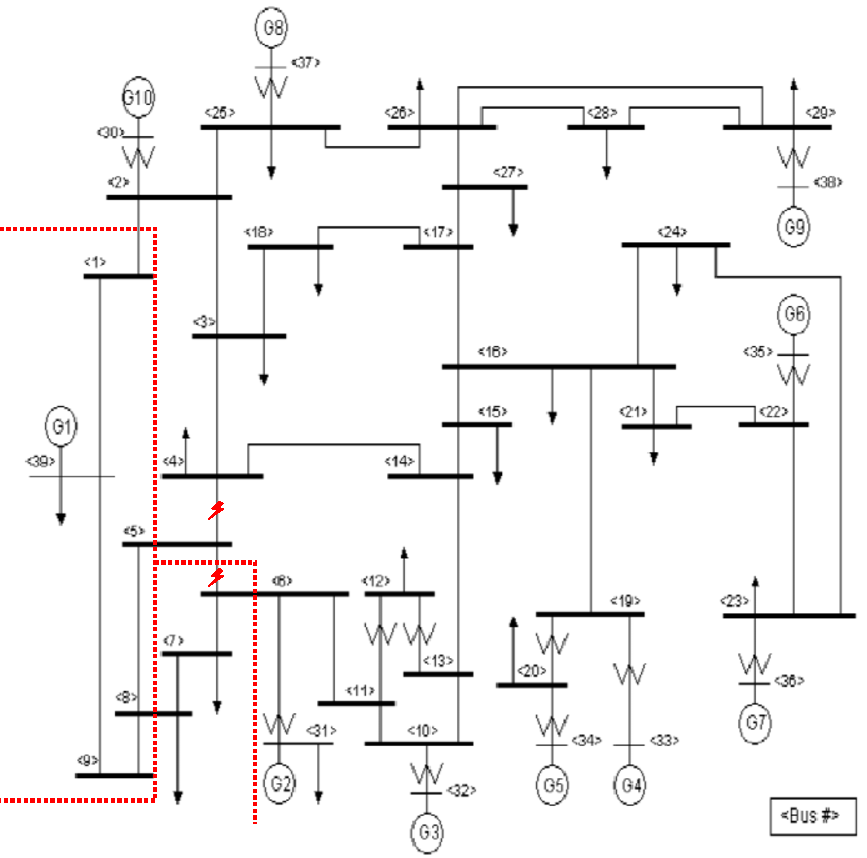
\includegraphics[width=0.475\linewidth]{Figs/IEEE39_slow_split.pdf}
        \label{subfig:split_slow}
    } \hfill
    \subfloat[System split following the (actual) fast sequence]{%
        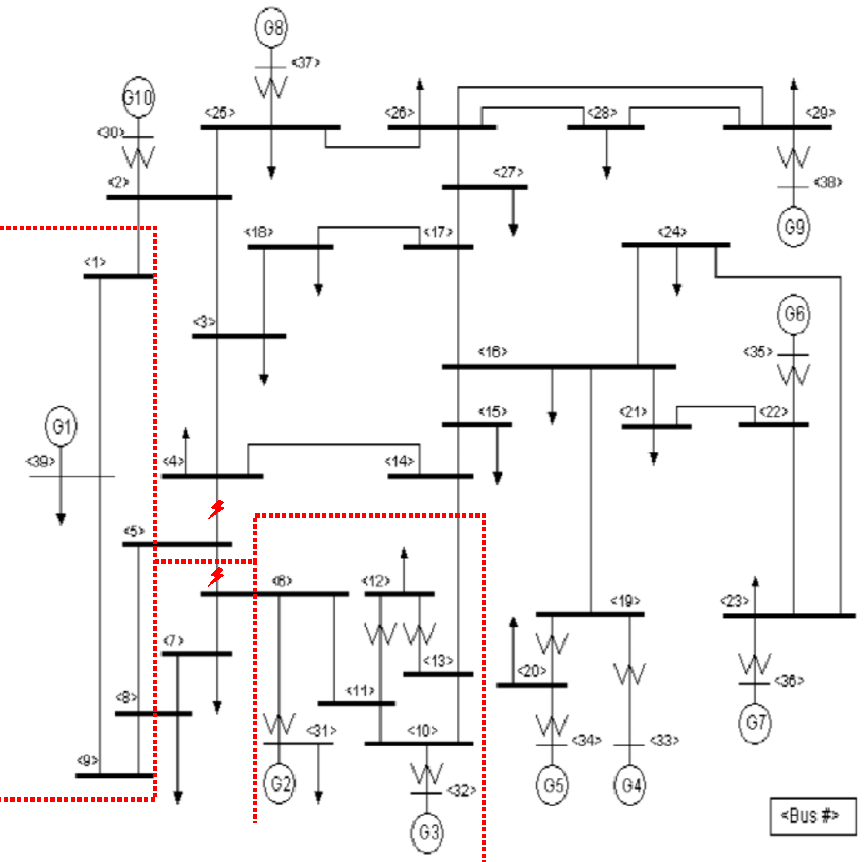
\includegraphics[width=0.475\linewidth]{Figs/IEEE39_fast_split.pdf}
        \label{subfig:split_fast}
    }
    \caption{Comparison of the consequences of the N-2 contingency of lines 5-6 and 6-7 in the slow and fast sequences}
    \label{fig:IEEE_split}
\end{figure}
}

% 6.15694 | 1-_2-1_AC_side2_DistanceSlow | Distance protection trip zone 2
% 6.22741 | 1-39-1_AC_side1_DistanceSlow | Distance protection trip zone 2
% 6.25709 | 5-_8-1_AC_side1_DistanceSlow | Distance protection trip zone 3
% 6.34501 | 8-_9-1_AC_side1_DistanceSlow | Distance protection trip zone 2
%
% 6.02905	13-14side1_Distance	Distance protection trip zone 3
% 6.05505 | 1-_2-1_AC_side2_DistanceFast | Distance protection trip zone 2
% 6.13181 | 5-_8-1_AC_side1_DistanceFast | Distance protection trip zone 3
% 6.134 | 1-39-1_AC_side1_DistanceFast | Distance protection trip zone 2
% 6.15187 | 4-14-1_AC_side2_DistanceFast | Distance protection trip zone 3
% 6.18391 | 8-_9-1_AC_side1_DistanceFast | Distance protection trip zone 2
%
% 6.02905	13-14side1_Distance	Distance protection trip zone 3
% 6.05505	1-2side2_Distance	Distance protection trip zone 2
% 6.13181	5-8side1_Distance	Distance protection trip zone 3
% 6.18407	8-9side1_Distance	Distance protection trip zone 2
% 8.27884	GEN___38_SM_Speed Under-speed protection trip
% 8.31923	GEN___37_SM_Speed	Under-speed protection trip
% 8.32712	GEN___30_SM_Speed	Under-speed protection trip
% 8.35866	GEN___33_SM_Speed	Under-speed protection trip
% 8.36521	GEN___35_SM_Speed	Under-speed protection trip
% 9.43916	23-24side1_Distance	Distance protection trip zone 2
% 9.55622	26-27side2_Distance	Distance protection trip zone 3
% 9.60304	16-17side1_Distance	Distance protection trip zone 3
% 9.81107	16-21side2_Distance	Distance protection trip zone 3
% 9.81712	GEN___33_SM_UVA	Under-voltage generator trip
% 9.84866	GEN___34_SM_UVA	Under-voltage generator trip

It can be noted that looking at the sequences of protection operations allows the indicator to perform significantly better than an indicator that would only consider the consequences of cascades. For example, Table~\ref{tab:indicator-consequence-based} shows the performance of an indicator that is true if the slower and faster sequences lead to different amount of load shedding%\footnote{Note that to estimate the load shedding, both sequences need to be simulated separately.}
. Such indicator indeed shows poor performance and misses between 20\% and 44\% (depending on the load model) of the sensitive contingencies.


\subsubsection{Causes of false negatives and false positives}
\label{sec:causesOfInaccuracy}

% 1s-restorative case, 3 FN
% _BUS___26-BUS___27-1_AC_end1-CB_end1-_BUS___26-BUS___29-1_AC
% Faster disconnection of GEN___38_SM_Speed that lost synchronism leads to less UFLS
% _BUS____2-BUS___25-1_AC_end2-CB_end2-_BUS___25-BUS___26-1_AC
% _BUS___26-BUS___29-1_AC_end2-CB_end1-_BUS___26-BUS___27-1_AC
% Same

% 5s, 1 FN
% _BUS___26-BUS___29-1_AC_end1-CB_end1-_BUS___26-BUS___27-1_AC
% Same

Table~\ref{tab:indicator} shows that the indicator misses 4 sensitive contingencies (3 false negatives in the 1s-restorative-load case, and 1 in the 5s-restorative one). In all those 4 cases, the difference between the slow and the (actual) fast sequences is that, in the fast sequence, generator 9 (bus 38) is disconnected faster by its protections after losing synchronism. This faster disconnection helps with frequency stability and leads to the activation of one less UFLS step. In the fast sequence estimated from the simulation of the slow one, this impact on the frequency behaviour is not caught, which leads to the false negatives. Using two simulations (one for the slower sequence and one for the faster sequence) would thus have lead to a null false negative rate (at the cost of an increase in computation time).

Table~\ref{tab:indicator} also shows that the indicator has a few false positives. It should however be noticed that false positives have a smaller impact that false negatives. Indeed, false negatives hide sensitive contingencies and lead to an inaccurate evaluation of their consequences (estimation from a single simulation while multiple MC simulations would be needed). However, false positives only cause unnecessary MC simulations which only affects computation time.

There are two causes for the occurrence of false positives. The first is that, in some cases, changing the order of protection operations does not impact the global evolution of the cascade. A typical example of this is when two distance protections operate to split the system in different points following an out-of-step condition. In this case, changing the order of protection operations will sometimes impact how the system splits and sometimes not.

The second cause is due to contingencies in which the operation of an additional protection system does not impact the consequences (in terms of load shedding). Most often, the protection system has no impact because it operates in an island that will collapse regardless of whether the protection system operates. % Both causes are each responsible for around 50\% of the false positives. % Also, one case where the ``new" protection that operates is Z3 instead of Z2 of the same protection -> actually not impact (most likely that Z2 will trip first anyway and that Z3 thus cannot trip after)


\section{Conclusion}
\label{sec:protection_conclusion}

Protection systems play a key role in maintaining highly-reliable power systems. However, they can sometimes misoperate, and they also impact (in positive and negative ways) the evolution of cascading outages. It is thus critical to model them adequately when performing probabilistic security assessments.

For this, it is important to first acknowledge the fact that protection systems can sometimes fail to clear faults in the normal way (i.e. by quickly disconnecting the faulted element), transforming mild N-1 contingencies into more severe N-k contingencies. This is because protection systems cannot be made 100\% dependable nor 100\% selective. Lack of dependability is mainly caused by the failure of individual protection elements (relays, breakers) and can be adequately modelled using standard reliability evaluation techniques such as fault trees and event trees. This is discussed in great detail in~\cite{GridPSA, Haarla}.

Lack of selectivity has more diverse causes, including design errors, incorrect settings, and as-left personnel errors~\cite{ProtectionMisoperationsBian2012} that are significantly harder to model. Most of the literature on the topic is rather old and is concerned with failure modes of legacy electromechanical relays that are no longer used. The update of failure models to digital relays is out of scope of this thesis but has recently been started in~\cite{Alexandre_PMAPS}. Statistics on the rate and causes of unselective protection behaviour at extra-high voltages (the ones most critical for security-related issues) would greatly help in evaluating the importance of unselective trips and to model them.

Beyond clearing the initial faults, protection systems also play a key role in how cascading outages propagate. As for fault clearing, lack of dependability or of selectivity can impact cascading outage evolution\footnote{Although, as will be shown in chapter~\ref{ch:DPSA}, the impact of lack of dependability after the initial fault clearing is relatively limited, except for SIPSs.}. However, even with perfectly reliable protection systems, it is difficult to predict how protection systems will impact the evolution of cascading outages. Indeed, during cascading outages, many protection systems might operate or be close to operate in a short window of time. Therefore, the propagation of cascading outages (and thus their final consequences) can be very sensitive to modelling uncertainties. In the literature, this has been studied using advanced MC techniques~\cite{SequencesRelaySobol, TwoLevelPSA}. However, MC simulations are computationally expensive which is problematic for the probabilistic security assessment of large systems that require to simulate many possible cascading outages. To alleviate this issue, this thesis proposes a simple indicator to predict which cascading outages are actually sensitive to protection-related uncertainties, so that MC simulations can be focused on these cases.

In conclusion, this chapter has discussed how to model N-k contingencies caused by protection misoperations and how to model the impact of protection systems on the evolution of cascading outages. The next step is thus to integrate this information into a comprehensive probabilistic security assessment framework. This is the objective of chapter~\ref{ch:DPSA}.

\chapter{Model of distribution grids}
\label{ch:distrib}
\minitoc

It has long been acknowledged that distribution grids can significantly impact the stability of transmission systems. This is especially true for voltage stability that strongly depends on the behaviour of loads following disturbances~\cite{CutsemBook, kundur}. However, most utilities still use relatively simple load models (e.g. compared to generator models) due to the difficulty to gather data on the loads connected to distribution grids.

This difficulty is caused by the fundamentally different nature of transmission and distribution grids. Indeed, a typical transmission grid connects dozens to hundreds of generators for which individual detailed models can be built (e.g. during the grid connection request and commissioning phases). Moreover, transmission system operators (TSOs) are also continuously made aware of the state of all generators (connection status, power output, etc.). Distribution grids however supply millions of customers each with their own appliances and behaviour. Therefore, only aggregated models can realistically be derived. The most commonly used load model is the ZIP load (aggregation of a constant impedance, a constant current, and a constant power load) and its derivates whose parameters are usually defined based on surveys and from transmission-level measurements of distribution grid behaviour following disturbances~\cite{IndustryLoadModel}.

%, and distribution system operators (DSOs) generally suffer from a lack of observability of their network.

% and their variable nature\footnote{Both the total amount of load and shares of different types of loads (heaters, motors, lamps, etc.) vary with the time of day and the season.}.

With the massive installation of distributed energy resources (DERs), distribution grids are playing a more and more active role in the stability and security of transmission systems. Currently, they have mostly a negative impact on system stability as they displace synchronous generation, thereby reducing system inertia and because they tend to disconnect themselves during system disturbances. For example, the frequency collapse of Italy in 2003 was partly caused by the unexpected disconnection of 3400~MW of DERs while the frequency was still above 49~Hz~\cite[p115]{Italy2003}. Similarly, DER disconnections also had a significant contribution in the 2019 UK power outage~\cite{2019UKBlackout}. In this case, 150~MW of DER was tripped as a direct consequence of the initial fault (lightning strike caused disconnection of DERs by vector-shift protection). Quickly after, between 350 and 430~MW of DERs were disconnected due to a high rate of change of frequency (RoCoF). At this point, a total of 1500~MW of generation was lost (around 500~MW of which were DERs), exceeding the primary reserve of 1000~MW which ultimately led frequency to drop to 48.8~Hz when under-frequency load shedding (UFLS) was activated. During the event, around 750~MW additional disconnection of DERs occurred due to frequency dropping below 49~Hz (protection of legacy DERs), UFLS activation (tripping entire feeders including DERs), and unknown causes. % On the other hand, there are perspectives regarding the provision of ancillary services by distributed generators.

As discussed in the previous chapters, performing a probabilistic security assessment requires to simulate the grid during severe disturbances and cascading outages. It is thus necessary to adequately model the behaviour of distribution grids during such disturbances and in particular the disconnection of DERs. Simple ZIP models are not able to do this, and more complex models are thus needed. To get better models, section~\ref{sec:distrib_review} reviews the load modelling literature and identifies an adequate modelling methodology. This methodology is then slightly modified in section~\ref{sec:distrib_methodology} and applied on two test cases.

In the first test case (section~\ref{sec:distrib_ISGT}), the methodology is applied on an academic test system to assess the accuracy of the developed load models in the simulation of cascading outages. In the second test case (section~\ref{sec:distrib_CIGRE}), the same methodology is used to study the impact of distribution grids on the transient stability of the Scottish transmission grid. This falls slightly out of scope of the thesis but demonstrates the lack of data issues encountered when modelling real distribution grids. Section~\ref{sec:distrib_conclusion} concludes this chapter with perspectives for future work.


\section{Load modelling review}
\label{sec:distrib_review}

Load modelling generally takes two steps: first, to define a load model, second, to define its parameters. The most commonly-used load models are reviewed in section~\ref{sec:load_models} and the techniques used to estimate their parameters are reviewed in section~\ref{sec:load_parameters}. Section~\ref{sec:distrib_review_conclusion} concludes this review with the techniques available to model distribution grids with large shares of DERs and a discussion of their limitations.


\subsection{Load models}
\label{sec:load_models}

Over the years, many load models have been developed for various studies. This section introduces the most popular ones, and redirect to the reviews of the CIGRE and NERC load modelling task forces~\cite{CIGREloadModels, NERCloadModelTF} for a more comprehensive and detailed review. The earliest and simplest load models were so-called ``static load models''. The behaviour of those loads directly depends on the current value of voltage and frequency, i.e.

\begin{IEEEeqnarray}{rCl}
    P & = & f_P(U, f) \\
    Q & = & f_Q(U, f)
\end{IEEEeqnarray}

This is as opposed to ``dynamic load models'' whose behaviour can also depend on time, the derivatives of voltage and frequency and on their past values. One of the most commonly-used static load models is the exponential load model whose behaviour is given by

\begin{IEEEeqnarray}{rCl}
    P & = & P_0 \left(\frac{V}{V_0}\right)^\alpha \\
    Q & = & Q_0 \left(\frac{V}{V_0}\right)^\beta
\end{IEEEeqnarray}

The active (resp. reactive) power consumption of this load is thus proportional the \(\alpha\)th (resp. \(\beta\)th) power of the ratio between the current voltage \(V\) and the initial (or reference) voltage \(V_0\). Particular values of \(\alpha\) and \(\beta\) are 0, 1, and 2 that respectively represent constant-power, constant-current, and constant-impedance loads.

In the 90s to 2010s, more complex load models were developed as some TSOs realised these simple load models did not allow reproducing historical blackouts in post-mortem analysis. The main element that was then added in load models was the induction motor. Indeed, induction motors represent a large share of load especially in industrialised countries and in regions with a lot of air conditioning. And these motors can have a large impact on voltage stability and small-signal stability. A simple load model including an induction motor is shown in Figure~\ref{fig:motorLoad}. This model consists of a constant-impedance load in parallel with an induction motor. The slip \(s\) of the motor is modelled with a classical swing equation.

\begin{IEEEeqnarray}{rCl}
    s & = & \frac{\omega_{ref} - \omega}{\omega_{ref}} \\
    2 H \frac{d\omega}{dt} & = & c_e - c_l
\end{IEEEeqnarray}
\noindent where \(\omega\) is the angular speed of the motor and \(omega_{ref}\) the angular speed of the grid, \(H\) is the inertia of the motor, and \(c_e\) and \(c_l\) are the electrical and load torques of the motor.

\begin{figure}
    \centering
    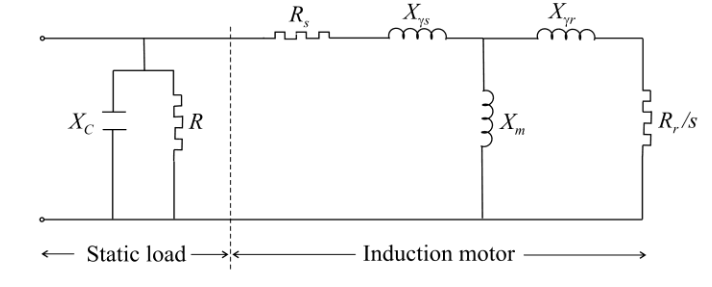
\includegraphics[width=0.6\linewidth]{Figs/MotorLoad.png}
    \caption{Constant impedance load in parallel with an induction motor~\cite{CIGREloadModels}}
    \label{fig:motorLoad}
\end{figure}

More complex load models have also been developed such as the WECC composite load model (CLM) shown in Figure~\ref{fig:WECC-CLM}. This model consists of a static (ZIP) load in parallel with 4 induction motors and an electronic load, all behind an equivalent feeder impedance. The electronic load is a constant power that can (partly) disconnect after severe voltage drops. The feeder model also includes an on-load tap changer to regulate distribution voltage on the long-term.

\begin{figure}
    \centering
    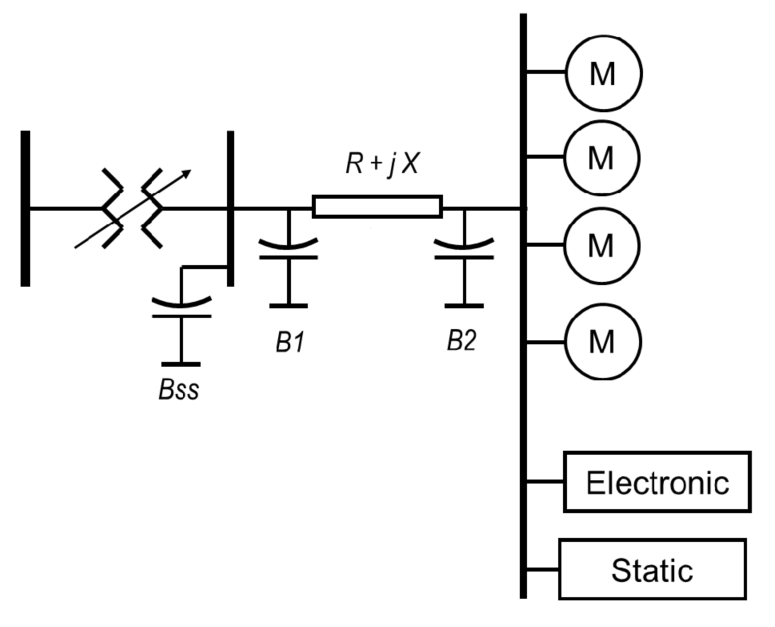
\includegraphics[width=0.5\linewidth]{Figs/WECC-composite-load-model.png}
    \caption{WECC composite load model~\cite{NERCloadModelTF}}
    \label{fig:WECC-CLM}
\end{figure}

The models presented above however do not consider distributed energy sources, and so, even more complex models have recently been developed. This is usually done by adding a DER model to an existing load model. For example, EPRI has developed a DER model called der\_a and recommends adding it to the WECC CML, at the end of the feeder (e.g. to represent rooftop solar) and/or at the start (e.g. to represent distribution-connected wind farms).

A large share of DERs consist of solar and wind generation, i.e. inverter-based generation. DERs are thus often represented with generic models as shown in Figure~\ref{fig:IBG}. These models represent (grid following) inverter-based generation as current-controlled sources with the following control blocks.

\begin{figure}
    \centering
    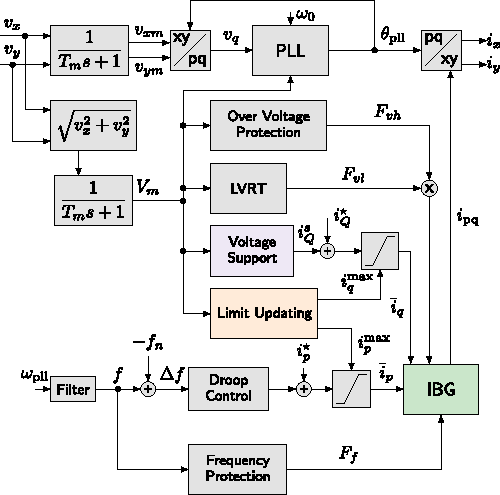
\includegraphics[width=0.6\linewidth]{Figs/IBG.pdf}
    \caption{Generic model of inverter-based generation, based on~\cite{Vorwerk}}
    \label{fig:IBG}
\end{figure}

\begin{itemize}
    \item Current limiter (Limit Updating) that limit the active and reactive current commands (\(i_P\) and \(i_Q\)) to keep the total current (\(\sqrt{i_P^2 + i_Q^2}\)) within the inverter ratings.
    \item Grid support blocks (Voltage support, Droop control) that help with voltage and frequency stability. These functions are usually not present in legacy inverters but are requested by recent grid codes (e.g.~\cite{G99}).
    \item Protection blocks (Over-Voltage Protection, Low-voltage ride-through (LVRT), Frequency Protections) that disconnect DERs during large disturbances. As DER model are used to represent many individual generators, it is necessary to account for the fact that only part of the generators might trip (legacy inverters more likely to trip than recent ones). These blocks thus multiply the current commands by factors between 0 and 1 (0 represent a complete trip of all generators, and 1, no trips).
    \item A phase-locked loop (PLL) and inverter model (IBG) to transform the active and reactive current commands to actual currents.
\end{itemize}

% One way to accurately model the interactions between the transmission and distribution sides of a grid is to perform simulations on complete a transmission and distribution network as in~\cite{FullTDexample}\footnote{To limit the size of the studied system, it is of course necessary to only consider the medium voltage level of the distribution grids, not the low voltage level.}. However, this approach cannot be used in this thesis due to the high computational power requirements of probabilistic dynamic security assessment. Outside the scope of this thesis, this approach also has issues of confidentiality and data handling.



\subsection{Estimating the parameters of load models}
\label{sec:load_parameters}

A model is only complete once numerical values have been assigned to its parameters. However, estimating the parameters that give the most accurate representation of the system might be difficult, especially since TSOs have little observability on distribution grids.


% \usepackage[edges]{forest}
% \begin{forest}
%     forked edges,
%     for tree={grow=south,draw,
%     font=\strut\footnotesize\sffamily\em},
%     [Load modelling
%         [Component-based approach]
%         [Parameter fitting
%             [Measurement-based]
%             [Simulation-based]]
%     ]
% \end{forest}

Two main types of methods exist to estimate the best parameters for load models: the component-based approach, and the parameter identification approach.

In the component-based approach, surveys, billing data and other data are used to estimate what is the share of the total load that is consumed by different types of loads. Commonly, loads are classified in residential, commercial, industrial, and agricultural loads. More refined classifications can also be used, for example, splitting industrial loads in petrochemical, mining, smelting, etc. Based on lab testing and validation with historical disturbances, parameters can be estimated for each of these load types. For example, when using the WECC CLM, NERC recommends modelling steel mills as loads with a 75\% motor share, a 20\% power electronic share, and a 5\% static load share. For server farms, it is instead 40\% of motors, and 60\% of power electronics~\cite{component_based}. The final parameters of the total load are then computed using weighted averages of the parameters of the various load subtypes. It should be noted that, as this process is quite complex (estimation of the share of different load types that vary with the time of day, and estimation of the load parameters for each load subtype), some form of sensitivity analysis should be performed to see how modelling uncertainties in load models affect the results of system studies.

In the parameter identification approach, the parameters of the load models are tuned such that the model behaves as closely as possible to some reference for a given set of disturbances. Mathematically speaking, this means finding the vector of parameters \(\bm{\theta}\) that minimises some sort of sum of square error between the behaviour of the load model and the behaviour of the reference as in the example formulation below.

\begin{IEEEeqnarray}{rCl}
\min_{\bm{\theta}} F(\bm{\theta}) & = & \frac{1}{d} \sum_{j=1}^d \left[F_P(\bm{\theta}, j) + F_Q(\bm{\theta}, j)\right] \\
%
\text{with } F_P(\bm{\theta}, j) & = &  \frac{1}{T} \sum_{t=1}^T \left[P(\bm{\theta}, j, t) - \hat{P}(j, t)\right]^2\\
%
F_Q(\bm{\theta}, j) & = &  \frac{1}{T} \sum_{t=1}^T \left[Q(\bm{\theta}, j, t) - \hat{Q}(j, t)\right]^2\\
%
\bm{\theta}^L \leq \bm{\theta} & \leq & \bm{\theta}^U
\end{IEEEeqnarray}
%
\noindent where \(P(\bm{\theta}, j, t)\) (resp. \(Q(\bm{\theta}, j, t)\)) is the active (resp. reactive) power consumed by the load model \(t\) time steps (out of \(T\)) after the occurrence of disturbance \(d\), and \(\hat{P}(j, t)\) (resp. \(\hat{Q}(j, t)\)) is the active (resp. reactive) power consumed by the reference at the same time and for the same disturbance. \(\bm{\theta^L}\) and \(\bm{\theta^U}\) are lower and upper bounds on the parameters of the load models used to guarantee that the load models gets realistic values.

The reference can either be time-series of measurements obtained after actual disturbances (measurement-based approach) or from detailed simulations (simulation-based approach). The measurement-based approach has the potential to give very accurate models as it is directly based on real measurements of the load behaviour. However, large disturbances are fortunately rare, so it might be difficult to obtain measurements for a sufficiently representative set of disturbances. Moreover, models obtained this way are only valid for one snapshot in time for which the measurement event occurred. The amount of PV disconnection will significantly vary between day and night times for example. Measurement-based approaches are thus mostly useful to validate the models obtained with other approaches\footnote{For small disturbances, developing models purely based on measurements is appropriate as small disturbances are more common and can be artificially created with transformer tap changes.} (the importance of model validation should however not be neglected).

In simulation-based approaches, distribution grids are simulated for a wide range of disturbances using a ``full model''. The results of these simulations are then used as a reference to tune the parameters of the load model (also called reduced model or dynamic equivalent). The challenge then becomes the definition of an appropriate full model. In many academic works, it has simply been assumed that such full model would be available~\cite{fulgencio}, i.e. that DSOs would have detailed dynamic models of their networks which is unrealistic.

In~\cite{ChaspierrePaper, ChaspierreThesis} however, this assumption has been strongly relaxed and authors assumed that only static data (i.e. branch impedances and resistances) would be available. For dynamic data, generic models were used for motors and DERs. The parameters of those dynamic models were assigned (relatively wide) probability density functions based on expert knowledge. Monte Carlo (MC) simulations were then performed to evaluate the impact of those uncertain dynamic parameters on the behaviour of loads. Finally, the parameters of the dynamic equivalents were fitted to match either the average behaviour of the uncertain full model. This is illustrated in Figure~\ref{fig:VDrop6}. In this figure, dotted lines show the results of MC simulations of a full distribution model following a voltage drop. From these simulations, the average behaviour can be estimated (brown full line), and the parameters of an equivalent can be fitted to match this average (brown dotted lines)\footnote{The MC simulations shown in Figure~\ref{fig:VDrop6} seem to aggregate around 2 main clusters: one with no or little trips of DERs (net load recovers to pre-fault values) and one with significant trips. This begs the question of why not clustering the results of MC simulations (e.g. using K-means) and building one equivalent per cluster. Some tests were performed in this direction, however, once multiple disturbances are considered, the separation between clusters becomes less obvious. Cluster centroids are then likely to miss extreme cases. The percentile-based approach is much more robust in this regard}.

However, Figure~\ref{fig:VDrop6} also shows that, due to high uncertainty, the actual load behaviour might strongly differ from the average expected behaviour. Building equivalents based on quantiles instead of averages might thus be more appropriate.

In~\cite{Vorwerk}, authors also used MC simulations to assess the impact of uncertainties of load behaviour. But, they then used machine-learning-based quantile forecasting to build an interval of potential load behaviour in addition to the mean behaviour. However, they only considered mild disturbances (load steps) and did not test their load model in transmission studies. Also, the final load model in~\cite{Vorwerk} is not a physical model but an artificial neural network whose behaviour is harder to interpret.

\begin{figure}
\centering
\begin{tikzpicture}
\pgfplotsset{width=0.7\linewidth}
\begin{axis}[
    xlabel={Time [s]},
    xmin=0, xmax=5,
    ylabel= {P [MW]},
    legend cell align=left,
    legend style={at={(1,0)},anchor=south east},
    ]

    \foreach \n in {0,...,49}{
        \addplot+ [mark=none, color=black, dotted, opacity=0.7, line width=0.6pt] table [x=time,y=VDrop6_\n] {Figs/VDrop6.txt};
    }
    \addplot+ [mark=none, line width=1pt, blue] table [x=time,y=Percentile5] {Figs/VDrop6Percentiles.txt};
    \addplot+ [mark=none, dashed, line width=1pt, blue] table [x=time,y=VDrop6] {Figs/VDrop6_5Fit.txt};
    \addplot+ [mark=none, line width=1pt, red] table [x=time,y=Percentile95] {Figs/VDrop6Percentiles.txt};
    \addplot+ [mark=none, dashed, line width=1pt, red] table [x=time,y=VDrop6] {Figs/VDrop6_95Fit.txt};
    \addplot+ [mark=none, line width=1pt, brown] table [x=time,y=VDrop6] {Figs/VDrop6_average.txt};
    \addplot+ [mark=none, dashed, line width=1pt, brown] table [x=time,y=VDrop6] {Figs/VDrop6_average_fit.txt}; % Actually this is the average of fit_5 and fit_95 because I don't want to resimulate it
    % \addlegendentry{Percentile 5}
    % \addlegendentry{Percentile 95}
    % \addlegendentry{Average}
    % \addlegendentry{5-equivalent}
    % \addlegendentry{95-equivalent}
    % \addlegendentry{MC samples}
    \legend{,,,,,,,,,,,,,,,,,,,,,,,,,,,,,,,,,,,,,,,,,,,,,,,,, MC samples,Percentile 5, 5-equivalent, Percentile 95, 95-equivalent, Average, Average equivalent}

\end{axis}
\end{tikzpicture}
\caption{Behaviour of the reduced (dashed lines) and unreduced (dotted and full lines) models of a distribution grid following a temporary voltage drop (disturbance 6 of Table~\ref{tab:disturbances}). The net load drawn after the drop is increased mainly due to disconnection of DERs (in uncertain amount).}
\label{fig:VDrop6}
\end{figure}

% \item Black-box approaches: in these methods, the model of a distribution system is an artificial neural network (ANN) that is trained to match the behaviour of the actual distribution system. These methods are quite popular since they do not require any information on the structure and components of the distribution grid. ANNs are thus most often matched to measurements of the behaviour of the distribution grid (often PMU measurements made at the point of common coupling (PCC) between the transmission and distribution grids). It is also possible to train ANNs from simulations of the distribution grid, but grey-box approaches (described below) are often preferred when one has enough information on the distribution grid to simulate it. The main limitation of measurement-based approaches (and by extension black-box approaches) is that large disturbances are rare. It is possible to intentionally introduce disturbances to generate more data but those disturbances are usually kept small for obvious reasons (usually tap changes or capacitor switching). Training ANNs for those disturbances is thus often impossible.
% \item Grey-box approaches: grey-box approaches are similar to black-box approaches except that the model used is a physical model instead of an ANN. The model usually has at most a few buses and should have a similar structure than the real grid\footnote{Taking the example shown in Figure~\ref{fig:greyBox}, if switches a and b are closed, and switch c is open, they grey-box model becomes two feeders in parallel. One feeder could represent a classical distribution system. The second, a large distribution-connected plant (with stricter connection requirements).}. The advantage is thus that results are more comprehensive, but it is necessary to known  the structure of the distribution grid. An example of grey-box model is shown in Figure~\ref{fig:greyBox}. Like black-box approaches, the parameters of the model are fitted to match the behaviour of the full model (e.g. in the least square sense). As it is not feasible to write the analytical formulation of the objective function (i.e. difference between behaviour of the grey-box and the real system), derivative-free optimisation methods (e.g. genetic algorithms, particle swarm optimisation) have to be used. The behaviour of the real system for a given operating point and disturbance can be obtained either from measurements or from simulations. As previously explained, only the simulation-based approach is appropriate when studying large disturbances\footnote{When available, measurements should still be used to validate the equivalent and/or the full distribution model.}.

    % \item Linear-based approaches: in these methods, the model of the full distribution network is first linearised. Then, different approaches (e.g. Hankel-norm approximation, modal approach, Krylov methods, etc.) allow to reduce the order of the linearised system. A theoretical bound on the error made by using the reduced-order model can be derived depending on the method used. These methods are however accurate only around a given operating point and are thus not appropriate to study large disturbances. These methods were originally developed to make reduced-order equivalents of neighbouring transmission systems. Indeed, TSOs mostly study the impact of disturbances originating in their own system. For moderately large disturbances, neighbouring TSOs are weakly affected, so a linearisation-based approach makes sense. Distribution systems however are much more dependent on their associated transmission system.
    % \item Coherency-based approaches: synchronous generators that tend to swing together are grouped into an equivalent machine. The network around those machines is then also reduced. Like linear-based approaches, these methods were developed to model neighbour transmission systems. They are often not applicable to distribution systems as synchronous generators are rarely used there.

% \begin{figure}
%     \centering
%     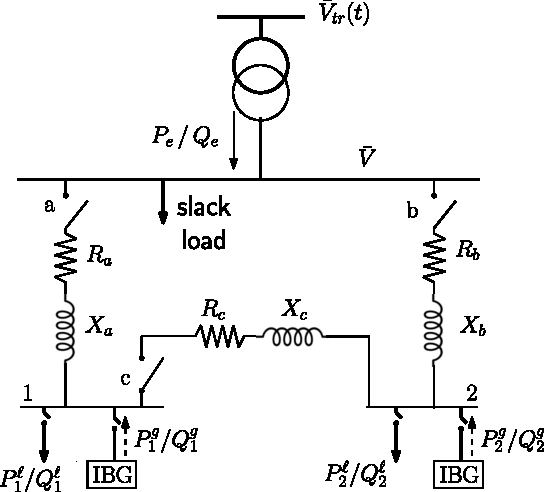
\includegraphics[width=0.6\linewidth]{Figs/GreyBoxEquivalent.pdf}
%     \caption{Possible grey-box equivalent topologies. Multiple topologies can be created from this scheme by changing the status of the switches~\cite{ChaspierreThesis}. IBG = Inverter-based generation}
%     \label{fig:greyBox}
% \end{figure}



\subsection{Conclusion}
\label{sec:distrib_review_conclusion}

This section reviewed three main approaches for load modelling (the component-based approach, the measurement-based approach, and the simulation-based approach) and discussed their advantages and limitations for simulating large disturbances. The component-based approach is the most popular amongst TSOs, however, it is rather involved, requiring to model potentially many types of load and to estimate their share in the total load. Moreover, it does not provide a direct way to perform sensitivity studies which are needed to validate this complex process.

The measurement-based approach is limited by the fact that large disturbances are rare. It should therefore be avoided when building load models from scratch. However, real measurements should definitively be used to validate the models obtained with other methods.

The main advantage of the simulation-based approach (at least the variants proposed in~\cite{ChaspierreThesis, ChaspierrePaper, Vorwerk}) is that it allows to easily perform sensitivity studies. This is generally important due to the complexity in developing adequate load models, but is even more important in the context of probabilistic security assessment. Indeed, probabilistic security assessments require simulating the system during cascading outages and very degraded states which challenges the accuracy of the (load) models used. The simulation-based approach is thus used in this thesis.

Section~\ref{sec:distrib_methodology} presents the load modelling methodology used in this thesis. As the methodology of~\cite{ChaspierreThesis, ChaspierrePaper} is quite powerful, it is used a strong basis for this work. The main difference is that this thesis uses percentiles instead of the average expected load behaviour.

Also, \cite{ChaspierreThesis, ChaspierrePaper} developed their models to study voltage stability issues and thus did not test their models for the simulation of cascading outages. And generally speaking, the majority of the literature on cascading outage simulation uses simple load models. Section~\ref{sec:distrib_ISGT} thus applies the methodology to the simulation of cascading outages on a standard test system.

% \begin{figure}
%     \centering
%     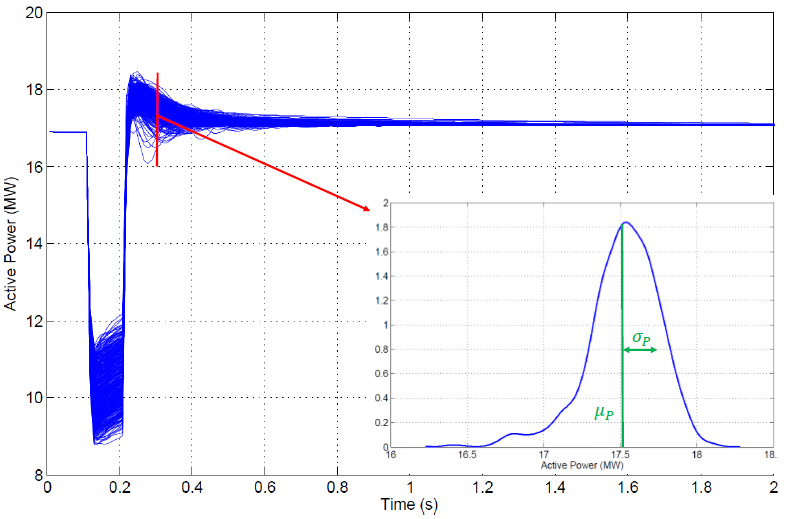
\includegraphics[width=0.6\linewidth]{Figs/GreyBoxUncertainty.png}
%     \caption{Average \(\mu_P\) and standard deviation \(\sigma_P\) of the active power consumption of a distribution grid following a disturbance at \(t=\)0.3~s~\cite[p58]{ChaspierreThesis}}
%     \label{fig:greyBoxUncertainty}
% \end{figure}


\section{Proposed load modelling approach}
\label{sec:distrib_methodology}

As stated, the methodology used in this thesis is strongly based on the one proposed in~\cite{ChaspierrePaper, ChaspierreThesis}. The methodology consists in two main parts. In the first part, a detailed model of the considered distribution grid is built. As modelling distribution grids is very complex, the parameters of the detailed model will be assigned very wide (and usually uniform) probability density functions based on expert knowledge (giving lower and higher realistic bounds for all parameters). MC simulations are then performed on a set of \(d\) disturbances to evaluate the impact of the uncertain modelling of the distribution grid on its behaviour.

Of particular interest are the active and reactive power at the point of common coupling (PCC) with the transmission grid. Thus, the following values are extracted from the MC simulations: \(\mathscr{P}_{P, i}(j, t)\) (resp. \(\mathscr{P}_{Q, i}(j, t)\)), the \(i\)th percentile over all MC simulations of the active (resp. reactive) during the \(j\)th disturbance at time \(t\); and \(\sigma_P(j,t)\) (resp. \(\sigma_Q(j,t)\)), the standard deviation of the active (resp. reactive) power for the same disturbance and at the same time.

In the second part, two dynamic equivalents of the distribution system model are built to bound the uncertain behaviour of the distribution grid: one (referred to as the 5-equivalent) that fits the 5th percentile of the active and reactive power of the distribution system, and one that fits the 95th percentile as shown in Fig.~\ref{fig:VDrop6}. Mathematically, the vector of parameters \(\bm{\theta}\) of each dynamic equivalent is taken as the solution of the following weighted least-square optimisation problem:

\begin{IEEEeqnarray}{rCl}
\label{eq:equivalent_optimisation}
\min_{\bm{\theta}} F(\bm{\theta}) & = & \frac{1}{d} \sum_{j=1}^d \left[F_P(\bm{\theta}, j) + F_Q(\bm{\theta}, j)\right] \\
%
\text{with } F_P(\bm{\theta}, j) & = &  \frac{1}{T} \sum_{t=1}^T \left[\delta_{i, P, j, t} \frac{P(\bm{\theta}, j, t) - \mathscr{P}_{P, i}(j, t)}{\sigma_P(j,t)}\right]^2\\
%
F_Q(\bm{\theta}, j) & = &  \frac{1}{T} \sum_{t=1}^T \left[\delta_{i, Q, j, t} \frac{Q(\bm{\theta}, j, t) - \mathscr{P}_{Q, i}(j, t)}{\sigma_Q(j,t)}\right]^2\\
%
\bm{\theta}^L \leq \bm{\theta} & \leq & \bm{\theta}^U
\end{IEEEeqnarray}
\noindent with \(i\) equals to 5 or 95. This formulation differs from the one in~\cite{ChaspierrePaper, ChaspierreThesis} only by the use of percentiles instead of the average behaviour. Also, the term \(\delta_{i, P, j, t}\) is added and is defined by

\begin{equation}
\delta_{5, P, j, t} = \left\{\begin{array}{lr}
    1 & \text{if } P(\bm{\theta}, j, t) \leq \mathscr{P}_{P, i}(j, t) \\
    \frac{1}{2} & \text{if } P(\bm{\theta}, j, t) > \mathscr{P}_{P, i}(j, t)
    \end{array}\right.
\end{equation}
\begin{equation}
\delta_{95, P, j, t} = \left\{\begin{array}{lr}
    1 & \text{if } P(\bm{\theta}, j, t) > \mathscr{P}_{P, i}(j, t) \\
    \frac{1}{2} & \text{if } P(\bm{\theta}, j, t) \leq \mathscr{P}_{P, i}(j, t)
    \end{array}\right.
\end{equation}

The term \(\delta_{i, Q, j, t}\) that has a similar definition. This factor results in a lower penalty for the equivalent that fits the 95th percentile if it consumes too much power and in a lower penalty for the 5-equivalent if it consumes too little. This leads to more conservative bounds on the behaviour of the distribution system. The main reason for adding this factor is that otherwise the numerical solution of the optimisation problem tends to converge to a solution that is closer to the average behaviour than expected. This is because it is usually easier to find a set of parameters to matches the average behaviour of the load model than its extremes.

Also, it should be noted that percentiles are computed individually for each disturbance and each point in time. Those percentiles are thus synthetic and represent an envelope of the possible behaviours of the distribution grid, not a likely behaviour which also makes it more complicated to find an optimal value for \(\bm{\theta}\).

Speaking of numerical solution, there is analytical formulation of \(P(\bm{\theta}, j, t)\) and its derivatives are difficult to estimate. A derivative-free approach is thus necessary to solve the optimisation problem. The differential evolution (DE) algorithm was used in~\cite{ChaspierreThesis, ChaspierrePaper} and is thus also used in this thesis. As it showed good performance, no other technique has been tested in this thesis. DE is stopped once sufficient accuracy is reached, i.e. when

\begin{equation}
    \label{eq:equivalent_stop}
    F_P(\bm{\theta}, j) \leq 1 \text{ and } F_Q(\bm{\theta}, j) \leq 1
\end{equation}

It should be noted that, \cite{ChaspierreThesis} developed a methodology to update the parameters of the load model when operating conditions change (e.g. if solar irradiation increase, the behaviour of the load will change as well as its parameters). However, for the sake of simplicity, load models were always parametrised from scratch in the test cases in this chapter.

% In~\cite{ChaspierreThesis}, a Least Absolute Shrinkage and Selection Operator (LASSO) was used in complement to DE in order to identify the parameters of the equivalent which are the most significant. This led to slow convergence in our case as more parameters deviate from their average value when fitting a 5th or 95th percentile than when fitting an average. If one wants to identify significant parameters, some form of sensitivity analysis might be more efficient.

% He also proposed a methodology to share the grey-box development between the TSO and DSOs to avoid confidentiality issues, and he discussed how to efficiently update the equivalent with varying operating conditions. Interestingly, he also proposed a control algorithm for a battery storage to be installed at the PCC to compensate for errors between the grey-box and the real system. Those elements are however not discussed further here.


It is common to ``train'' an equivalent by connecting it to an infinite bus to which voltage (and possibly angle and frequency) disturbances are applied~\cite{ChaspierreThesis, CIGREloadModels, fulgencio}. However, in this thesis, it was found that connecting it to a synchronous machine that has roughly the same rating as the total gross load through a line with an impedance of 0.1~pu leads to equivalents which are more accurate in transmission studies. This is because it allows for easier incorporation of fault-induced delayed voltage recovery events into the training set of the equivalent. Also, it makes \(P(\bm{\theta}, j, t)\) more sensitive to \(\bm{\theta}\). This is further discussed in section~\ref{sec:isgt_results_visual}.

It should be noted that the synchronous machine and line do not aim to be an equivalent of the transmission system as seen from the distribution system. As will be shown in section~\ref{sec:distrib_ISGT}, equivalents built this way have a very good accuracy even when used at different locations with different system strengths, and during cascading outages during which the system strength at a given location can significantly vary\footnote{Other modifications were made compared to~\cite{ChaspierreThesis} in order to help the convergence of DE and are listed below. However, additional tests should be performed to validate the relevance of those modifications.
\begin{itemize}
    \item \cite{ChaspierreThesis} uses a least absolute shrinkage and selection operator (LASSO) to identify the most important parameters of the equivalents. This works by adding a penalty in the objective function when identified parameters deviate from their expected value (average of \(\bm{\theta}^L\) and \(\bm{\theta}^U\)), and decreasing the penalty until a solution that satisfies (\ref{eq:equivalent_stop}) is found. This works well for the average equivalent, but for the 5- and 95-equuivalents, many parameters deviate from their expected value which slows down convergence and requires to use a small penalty term. Most parameters are then identified as critical by the LASSO.
    \item \cite{ChaspierreThesis} iteratively added disturbances to (\ref{eq:equivalent_optimisation}), stopping early if the equivalent trained with a small set of disturbances was valid (i.e. satisfied (\ref{eq:equivalent_stop})) for all disturbances. In this work however, it was necessary to train using many disturbances to correctly fit the tripping parameters, so it was faster to directly train the equivalent will all considered disturbances.
\end{itemize}
}.


The training disturbances used in this work are impedant short-circuits of different durations applied at the PCC leading to more or less severe voltage drops as listed in Table~\ref{tab:disturbances}. More or less impedant short-circuit represent faults that are more or less far away from the load. Additionally, if the equivalent is to be used in a case where the frequency goes outside the [49, 51]~Hz range (cascading outages), frequency ramps are added to the training disturbances to fit the frequency related parameters of the equivalent. 4 ramps are considered here, going respectively from 50~Hz to 47.5, 48.5, 51.5, and 52.5~Hz, all in 1.5s.

\begin{table}
\centering
\caption{Training disturbances}
\label{tab:disturbances}
\begin{tabular}{@{}ccc@{}}
\toprule
Id & Voltage dip (pu) & Duration (ms) \\ \midrule
1  & 0.2               & 100           \\
2  & 0.2               & 200           \\
3  & 0.3               & 100           \\
4  & 0.3               & 200           \\
5  & 0.4               & 100           \\
6  & 0.4               & 200           \\
7  & 0.5               & 100           \\ \bottomrule
\end{tabular}
% \hfill
\hspace{1cm}
\begin{tabular}{@{}ccc@{}}
\toprule
Id & Voltage dip (pu) & Duration (ms) \\ \midrule
8  & 0.5               & 200           \\
9  & 0.7               & 100           \\
10 & 0.7               & 200           \\
11 & 0.8               & 200           \\
12 & 0.8               & 500           \\
13 & 0.9               & 500           \\
14 & 0.9               & 1000          \\ \bottomrule
\end{tabular}
\end{table}


\section{Test case 1: Simulation of cascading outages}
\label{sec:distrib_ISGT}

\begin{tcolorbox}[width=\linewidth, sharp corners=all,
    colback=white!80!black,
    colframe=white!80!black]
This section is partly based on the following publication:
\begin{itemize}
    \item \fullcite{ISGT2023_ADN}
\end{itemize}
\end{tcolorbox}


The objective of this test case is to study if the dynamic equivalencing methodology proposed in~\ref{sec:distrib_methodology} is adequate to study cascading outages. To do this, simulations of cascading outages will first be performed on a complete model of an academic transmission and distribution system (i.e. complete grid model from 400~kV to 20~kV), then the same simulations will be performed but replacing the distribution grid models by simpler equivalents. The distribution grid models used in this test case are described in section~\ref{sec:isgt_distrib} and the complete transmission and distribution grid model is described in section~\ref{sec:isgt_TD}. The simulations results obtained with the full and reduced distribution models are compared in section~\ref{sec:isgt_results}

\subsection{Distribution system}
\label{sec:isgt_distrib}

The distribution system considered in this test case is based on the CIGRE medium voltage (MV) network\footnote{Static data is available for this network. However, the methodology is very generic and could still be applied if the static data was uncertain. This is performed in the second test case (section~\ref{sec:distrib_CIGRE})}~\cite{CIGREMV} shown in Figure~\ref{fig:CIGRE_MV}. Loads 1 and 12 (that account for almost 90\% of the total load) have been removed as they represent separate feeders and do not include data on DERs. The distribution transformers have been downscaled to match the original voltage profile. Finally, the PV and wind installations have been upscaled to reach each 40\% of the total load. Results presented in this section were obtained at an operating point with 100\% wind availability and 25\% solar availability, leading to an instantaneous inverter-based generation (IBG) penetration of 50\%.


\begin{figure}
\centering
\subfloat[CIGRE MV network with solar and wind generation~\cite{CIGREMV}]{%
    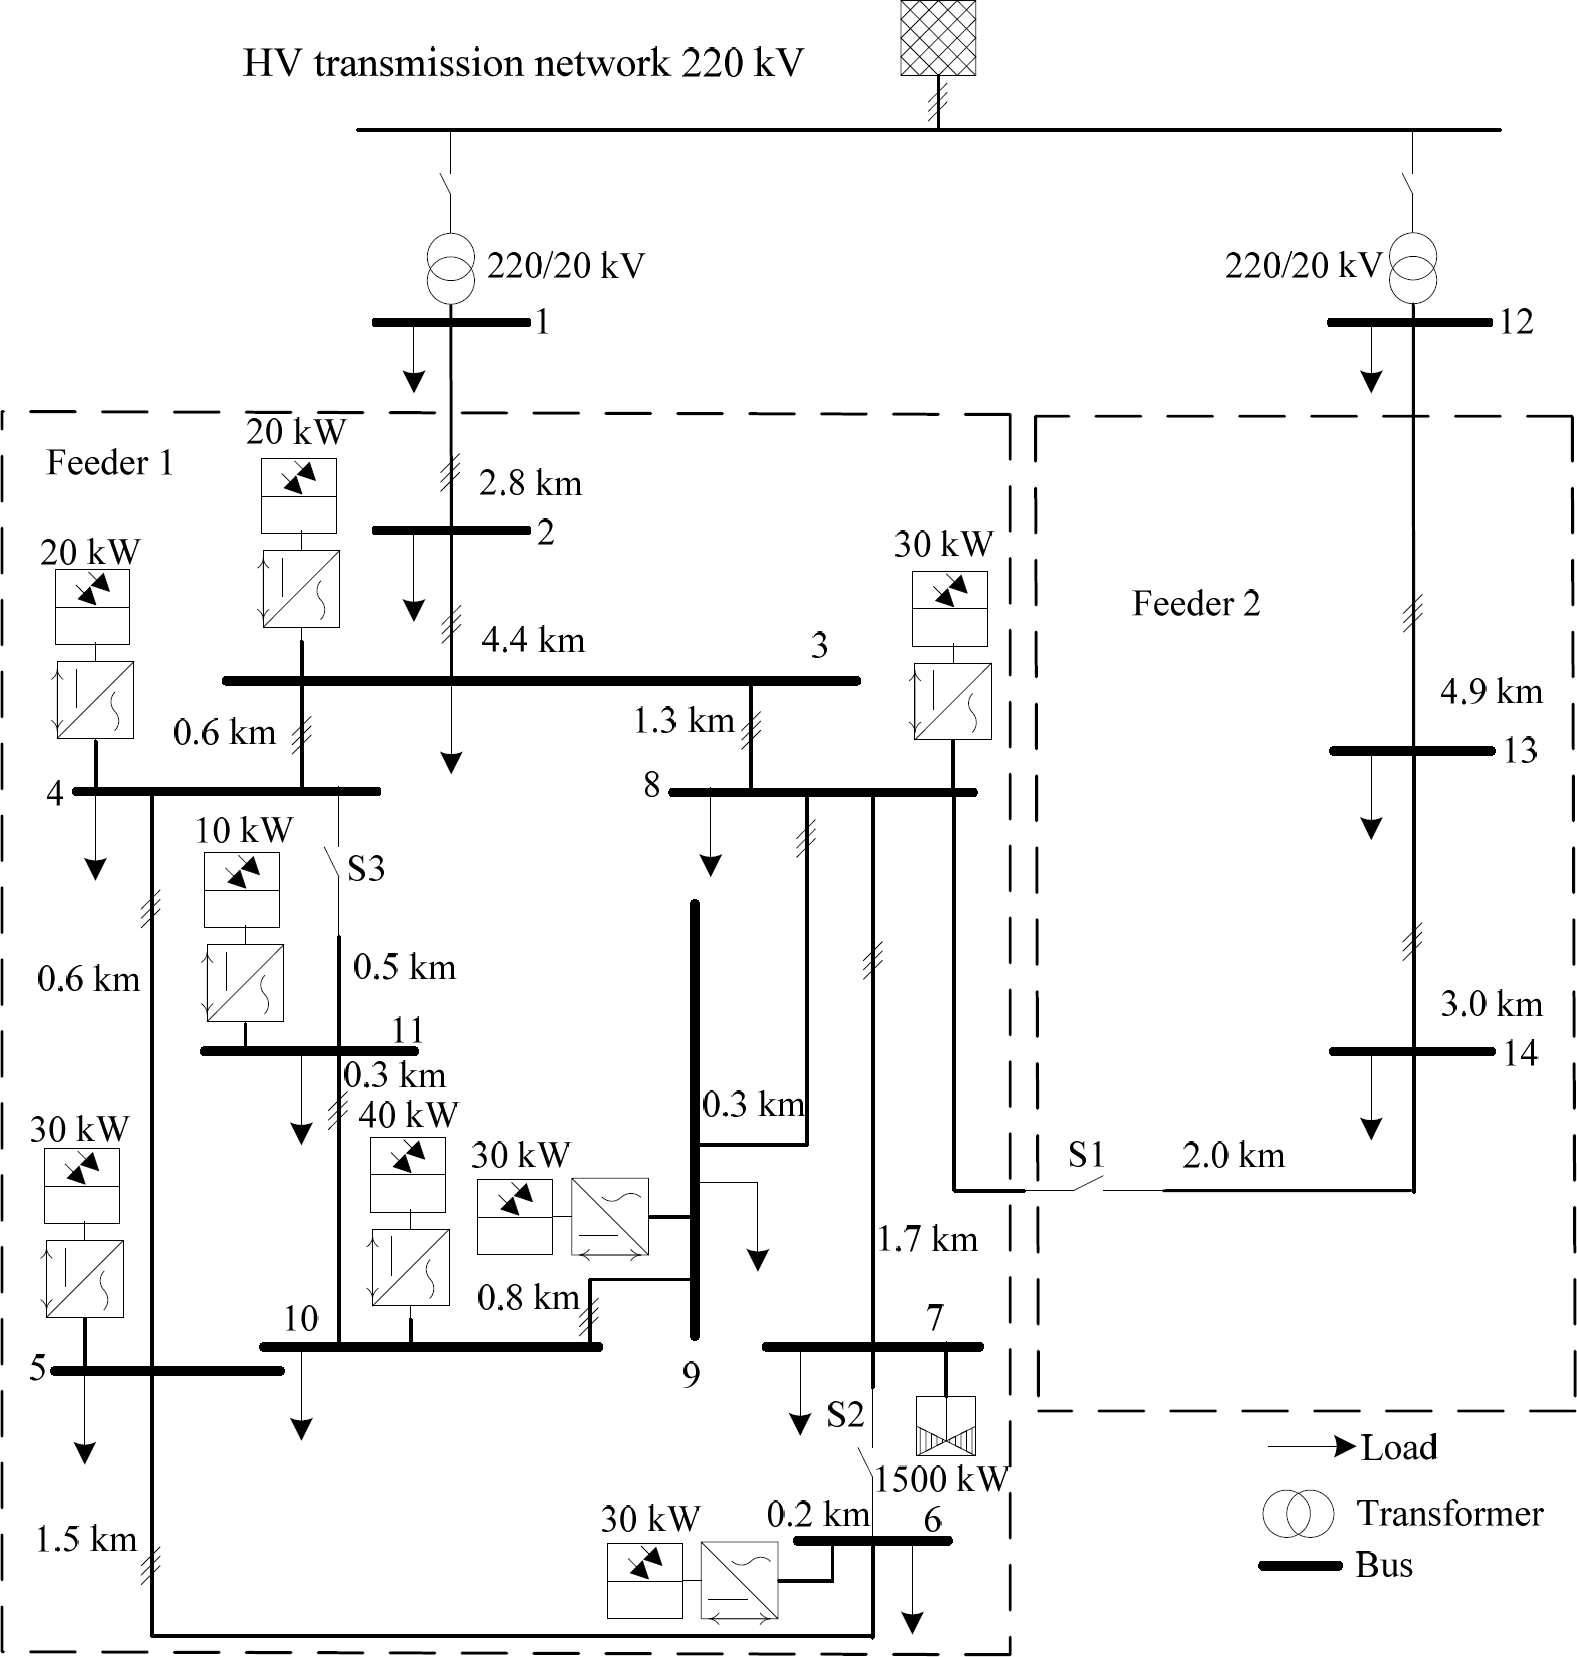
\includegraphics[width=0.6\linewidth]{Figs/cigre_network_mv.png}
    \label{fig:CIGRE_MV}
    } \hfill
\subfloat[Dynamic equivalent]{%
    \begin{tikzpicture}[scale = 0.8, transform shape]

    \draw [line width=0.7mm](6,1.5) -- (8,1.5);
    \draw (7,2.5) node[gridnode](extgrid){};
    \draw (7,2) to [short] (7,1.5);

    \draw (7,1.5) to [oosourcetrans] (7,0);
    \draw [line width=0.7mm](6,0) -- (8,0);
    \draw (7,0) to [short] (7,-2);
    \draw [line width=0.7mm](5,-2) -- (10,-2);

    \draw [-{Latex[scale=0.7]}] (6.5,0) -- (6.5,-0.4);
    \draw [-{Latex[scale=3]}] (5.5,-2) -- (5.5,-4);
    \draw (6.5,-3.5) node[elmech](M1){M};
    \draw (7.5,-3.5) node[elmech](M1){M};
    \draw (6.5,-3) to [short] (6.5,-2);
    \draw (7.5,-3) to [short] (7.5,-2);

    \draw (8.1,-3.8) rectangle (8.9,-3.2) node[midway] {IBG};
    \draw (9.1,-3.8) rectangle (9.9,-3.2) node[midway] {IBG};
    \draw (8.5,-3.2) to [short] (8.5,-2);
    \draw (9.5,-3.2) to [short] (9.5,-2);

    \end{tikzpicture}
    \label{fig:Equivalent}
    }
\caption{Distribution systems used in test case 1}
\label{fig:distrib}
\end{figure}

The dynamic equivalent of the distribution system is a relatively simple model made of one load bus connected to the transmission grid by an equivalent impedance and a distribution transformer as shown in Fig.~\ref{fig:Equivalent}. The load bus consists of an exponential load, two first-order inductor motor models (to allow for partial stalling of motors), and two IBG models (one that represents PV units, and one that represents wind).

The IBG model used in the full and reduced distribution models is the one shown in Figure~\ref{fig:IBG} and described in more details in~\cite{ChaspierreThesis}\footnote{The partial tripping models have been slightly modified compared to~\cite{ChaspierreThesis} in order to allow the equivalent model to more accurately fit the behaviour of the distribution system. Please refer to the model implementation available in \url{https://fredericsabot.github.io/Publications.html} for more information.}.

\subsection{Transmission \& distribution network}
\label{sec:isgt_TD}

The complete transmission and distribution (T\&D) system considered is built by replacing all loads of the IEEE 39-bus test system (except load 39 which represents an interconnection) by copies of the CIGRE MV network. Each of those copies is scaled such that its gross load is the same as the load it replaces in the 39-bus system. This leads to a reduction of the net load seen on the transmission side (from 6100~MW to 3600~MW) as DERs are now satisfying part of the total load. To account for this, generators 33, 34, and 36 (coal units) are disconnected and the setpoint of generator 39 is reduced from 1000~MW to 263~MW. To keep the system N-1 secure, a synchronous compensator is added in place of generator 33, and generator 38 is equipped with a faster AVR. The same protection system models (and associated uncertainty) as in section~\ref{sec:protection_test_case} are used.

\subsection{Results}
\label{sec:isgt_results}

The validation of the equivalencing process is made in multiple steps. First, a simple visual comparison of time-domain evolution of the transmission system simulated with full and reduced models of distribution grids is performed as a first intuitive validation and to highlight the importance of correctly training the equivalents. This is performed in section~\ref{sec:isgt_results_visual}. Then, section~\ref{sec:isgt_results_CCT} validates the reduced models for the purpose of a classical transmission system study: the evaluation of generator critical clearing times. Finally, section~\ref{sec:isgt_results_cascading} performs a validation for the actual use case of this thesis: the simulation of cascading outages.


\subsubsection{Visual comparison}
\label{sec:isgt_results_visual}

As stated above, it is common to train equivalents by connecting them to an infinite-bus system to which disturbances are applied. However, this led to inaccurate equivalent models in this thesis. Indeed, Figure~\ref{fig:fault39} shows a significant discrepancy between the voltage evolution at bus 4 following a 100ms fault at bus 39 (that is relatively far from bus 4) simulated with the full distribution models (dotted lines) and the one simulated with reduced models trained with an infinite bus (dashed lines). Most notably, there is a large voltage spike after fault clearing when simulating the system evolution with the 5-equivalent.

This spike is mainly caused by an inadequate value for the parameter \(I_{max}\), the rated current of IBGs. This parameter is quite important as it limits the reactive power support that can be delivered by IBGs during voltage recovery. It has however a lower importance when training with an infinite bus since the voltage is imposed. It is thus better to train the equivalents by connecting them to a source with finite strength. In this thesis, this was done by connecting the equivalents to a small synchronous machine rated to the gross load of the equivalent through a 0.1~pu impedance (line). The voltage drops imposed on the infinite bus are thus replaced by short-circuit at the point of common coupling. The short-circuit impedance is selected to create the same voltage drops as in Table~\ref{tab:disturbances}.

Figure~\ref{fig:fault39} shows that the equivalents trained this way allow to better match the results obtained with the full distribution model. Figure~\ref{fig:fault29} shows similar results but for a close-in fault. The same voltage overestimation is done by the 5-equivalent trained with an infinite bus. And the 5- and 95- equivalents trained with a small synchronous machine provide a good envelope of the results obtained with full distribution models. In the remaining of this thesis, all equivalents are thus trained this way.

% \TODO{Fig of equivalent with average parameters vs. correct ones (in draft of ISGT paper), not fully accurate but already way better than simple load model}


% \begin{figure}
% \centering
% \begin{tikzpicture}
% \pgfplotsset{width=\linewidth}
% \begin{axis}[
%     xlabel={Time [s]},
%     xmin=0, xmax=10,
%     ylabel= {Voltage at bus 4 [pu]},
%     legend cell align=left,
%     legend style={at={(0,0)},anchor=south west},
%     ]
%
%     \addplot+ [mark=none] table [x=time_5,y=V4_5] {Figs/4_100ms_Bounds.txt};
%     \addplot+ [mark=none] table [x=time_95,y=V4_95] {Figs/4_100ms_Bounds.txt};
%     \addplot+ [mark=none, dashed, green] table [x=time_5,y=V4_5] {Figs/4_100ms_BoundsInf.txt};
%     \addplot+ [mark=none, dashed, orange] table [x=time_95,y=V4_95] {Figs/4_100ms_BoundsInf.txt};
%     \foreach \n in {0,...,49}{
%         \addplot+ [mark=none, color=black, dotted, opacity=0.3] table [x=time,y=V4_\n] {Figs/4_100ms_Random.txt};
%     }
%     \addlegendentry{Percentile 5}
%     \addlegendentry{Percentile 95}
%     \addlegendentry{Percentile 5}
%     \addlegendentry{Percentile 95}
%     \addlegendentry{MC samples}
%
% \end{axis}
% \end{tikzpicture}
% \caption{Comparison between the full TD (dotted lines), dynamic equivalent trained using an infinite bus (dashed lines) and dynamic equivalent trained using a small transmission system (full lines) models: voltage evolution following a 100ms fault at bus~4}
% \label{fig:fault4}
% \end{figure}
%
%
% \begin{figure}
% \centering
% \begin{tikzpicture}
% \pgfplotsset{width=\linewidth}
% \begin{axis}[
%     xlabel={Time [s]},
%     xmin=0, xmax=10,
%     ylabel= {Voltage at bus 4 [pu]},
%     legend cell align=left,
%     legend style={at={(0,0)},anchor=south west},
%     ]
%
%     \addplot+ [mark=none] table [x=time_5,y=V16_5] {Figs/16_100ms_Bounds.txt};
%     \addplot+ [mark=none] table [x=time_95,y=V16_95] {Figs/16_100ms_Bounds.txt};
%     \addplot+ [mark=none, dashed, green] table [x=time_5,y=V16_5] {Figs/16_100ms_BoundsInf.txt};
%     \addplot+ [mark=none, dashed, orange] table [x=time_95,y=V16_95] {Figs/16_100ms_BoundsInf.txt};
%     \foreach \n in {0,...,49}{
%         \addplot+ [mark=none, color=black, dotted, opacity=0.3] table [x=time,y=V16_\n] {Figs/16_100ms_Random.txt};
%     }
%     \addlegendentry{Percentile 5}
%     \addlegendentry{Percentile 95}
%     \addlegendentry{Percentile 5}
%     \addlegendentry{Percentile 95}
%     \addlegendentry{MC samples}
%
% \end{axis}
% \end{tikzpicture}
% \caption{Comparison between the full TD (dotted lines), dynamic equivalent trained using an infinite bus (dashed lines) and dynamic equivalent trained using a small transmission system (full lines) models: voltage evolution following a 100ms fault at bus~16}
% \label{fig:fault16}
% \end{figure}

\begin{figure}
\centering
\begin{tikzpicture}
\pgfplotsset{width=0.7\linewidth}
\begin{axis}[
    xlabel={Time [s]},
    xmin=0, xmax=10,
    ylabel= {Voltage at bus 4 [pu]},
    legend cell align=left,
    legend style={at={(0,0)},anchor=south west,
        cells={align=left}}, % Needed to have line breakers in legend
    ]

    \addplot+ [mark=none] table [x=time_5,y=V1_5] {Figs/39_100ms_Bounds.txt};
    \addplot+ [mark=none] table [x=time_95,y=V1_95] {Figs/39_100ms_Bounds.txt};
    \addplot+ [mark=none, dashed, green] table [x=time_5,y=V1_5] {Figs/39_100ms_BoundsInf.txt};
    \addplot+ [mark=none, dashed, orange] table [x=time_95,y=V1_95] {Figs/39_100ms_BoundsInf.txt};
    \foreach \n in {0,...,49}{
        \addplot+ [mark=none, color=black, dotted, opacity=0.3] table [x=time,y=V1_\n] {Figs/39_100ms_Random.txt};
    }
    \addlegendentry{5-equivalent  \\ (small machine training)}
    \addlegendentry{95-equivalent \\ (small machine training)}
    \addlegendentry{5-equivalent  \\ (infinite-bus training)}
    \addlegendentry{95-equivalent \\ (infinite-bus training)}
    \addlegendentry{MC samples \\ (full T\&D model)}

\end{axis}
\end{tikzpicture}
\caption{Voltage evolution at bus 4 for a 100ms fault at bus 39 simulated with full distribution models (dotted lines), with reduced models trained with an infinite-bus system (dashed lines), and with reduced models trained with a small synchronous machine (full lines)}
\label{fig:fault39}
% \end{figure}
\vspace{0.8cm}
% \begin{figure}
\centering
\begin{tikzpicture}
\pgfplotsset{width=0.7\linewidth}
\begin{axis}[
    xlabel={Time [s]},
    xmin=0, xmax=10, ymin = 0.8,
    ylabel= {Voltage at bus 29 [pu]},
    legend cell align=left,
    legend style={at={(0,0)},anchor=south west,
        cells={align=left}}, % Needed to have line breakers in legend
    ]

    \addplot+ [mark=none] table [x=time_5,y=V4_5] {Figs/29_100ms_Bounds.txt};
    \addplot+ [mark=none] table [x=time_95,y=V4_95] {Figs/29_100ms_Bounds.txt};
    \addplot+ [mark=none, dashed, green] table [x=time_5,y=V4_5] {Figs/29_100ms_BoundsInf.txt};
    \addplot+ [mark=none, dashed, orange] table [x=time_95,y=V4_95] {Figs/29_100ms_BoundsInf.txt};
    \foreach \n in {0,...,49}{
        \addplot+ [mark=none, color=black, dotted, opacity=0.3] table [x=time,y=V4_\n] {Figs/29_100ms_Random.txt};
    }
    \addlegendentry{5-equivalent  \\ (small machine training)}
    \addlegendentry{95-equivalent \\ (small machine training)}
    \addlegendentry{5-equivalent  \\ (infinite-bus training)}
    \addlegendentry{95-equivalent \\ (infinite-bus training)}
    \addlegendentry{MC samples \\ (full T\&D model)}

\end{axis}
\end{tikzpicture}
\caption{Voltage evolution at bus 29 for a 100ms fault at bus 29 simulated with full distribution models (dotted lines), with reduced models trained with an infinite-bus system (dashed lines), and with reduced models trained with a small synchronous machine (full lines)}
\label{fig:fault29}
\end{figure}

% \begin{figure}
% \centering
% \begin{tikzpicture}
% \pgfplotsset{width=\linewidth}
% \begin{axis}[
%     xlabel={Time [s]},
%     xmin=0, xmax=5,
%     ylabel= {Power at PCC [MW]},
%     legend cell align=left,
%     legend style={at={(1,0)},anchor=south east},
%     ]
%
%     \addplot+ [mark=none] table [x=time,y=V1] {Figs/Average_equivalent_1.txt};
%     \foreach \n in {0,...,19}{
%         \addplot+ [mark=none, color=black, dotted, opacity=0.5] table [x=time,y=V1_\n] {Figs/Training_Random_1.txt};
%     }
%     \addlegendentry{Equivalent}
%     \addlegendentry{MC samples}
%
% \end{axis}
% \end{tikzpicture}
% \caption{Performance of an equivalent with guessed parameters: disturbance 1 (even more difficult to estimate tripping parameters)}
% \label{fig:average-equivalent}
% \end{figure}


\subsubsection{Comparison of critical clearing times}
\label{sec:isgt_results_CCT}

This section compares the critical clearing times (CCT) of the generators of the IEEE 39-bus test system when loads are modelled either using a full distribution system model (full T\&D simulations), using dynamic equivalents, and using a simple restorative load model (netted loads, same model as in (\ref{eq:restorative_load_model_1})-(\ref{eq:restorative_load_model_2})). For fairness of the comparison, the parameters of the restorative load models have been tuned to match either the 5th or 95th percentile behaviour of the full distribution system model\footnote{The same training process is used for the simple restorative load than for the dynamic equivalents. However, the disturbances that lead to DER disconnection are not included in the training set as the simple load model cannot account for them.}.

% For the full T\&D simulations, 90\% confidence intervals of those CCTs are computed based on 50 MC simulations. Actually, for each CCT, two (90\%) confidence intervals are built. The ``dependent (dep.) confidence interval'' that is computed by assigning the same random parameters in all copies of the CIGRE MV network, and the ``independent (ind.) confidence interval'' where random values are sampled independently for each copy.

% Table~\ref{tab:CCT} compares those intervals to the bounds obtained with dynamic equivalents. The bounds obtained with the equivalents are defined as the range between the CCT computed when all loads are replaced by their ``5-equivalent" and the CCT computed with the ``95-equivalents". Bounds are obtained in the same way for the restorative load models.


Table~\ref{tab:CCT} compares the 90\% confidence intervals of those CCTs computed with probabilistic T\&D simulations to the bounds obtained with dynamic equivalents. The bounds obtained with the equivalents are defined as the range between the CCT computed when all loads are replaced by their ``5-equivalent" and the CCT computed with the ``95-equivalents". Bounds are obtained in the same way for the netted load model.


\begin{table}
\centering
\caption{CCTs computed using dynamic equivalents, probabilistic T\&D simulations, and a simple netted load model}
\label{tab:CCT}
\begin{tabular}{@{}ccccccc@{}}
\toprule
\multirow{2}{*}[-0.5ex]{Generator} &
\multicolumn{4}{c}{CCT 5-95 bounds (ms)} &
\multirow{2}{*}[-0.5ex]{\(^a\)} &
\multirow{2}{*}[-0.5ex]{\(^b\)} \\ \cmidrule(lr){2-5}
   & Equivalents   & T\&D dep. & T\&D ind.  &  Netted load    \\ \midrule
30 & [550, 616]    & [554, 631]    & [583, 610] & [600, 604] & 72  & 100 \\
31 & [240, 264]    & [244, 255]    & [247, 252] & [234, 234] & 100 & 100 \\
32 & [200, 214]    & [200, 210]    & [204, 210] & [194, 194] & 98  & 100 \\
35 & [214, 244]    & [220, 234]    & [224, 230] & [210, 222] & 100 & 100 \\
37 & [244, 264]    & [242, 260]    & [250, 254] & [244, 244] & 94  & 100 \\
38 & [180, 210]    & [184, 194]    & [184, 190] & [180, 180] & 100 & 100 \\
39 & [634, stable] & [648, stable] & stable & stable & 100 & 100 \\ \bottomrule
\end{tabular} \\ \vspace{0.1cm}
\footnotesize{\(^a\) (resp. \(^b\)) Percentage of dependent (resp. independent) T\&D samples that lead to a CCT that is within the 5-95 range computed using the equivalent.}
\end{table}

% % Simplified version for short presentations (1)
%
% \begin{table}
% \centering
% \caption{Comparison of critical clearing times}
% \resizebox{\linewidth}{!}{%
% \begin{tabular}{@{}ccccc@{}}
% \toprule
% \multirow{2}{*}[-0.5ex]{Generator} &
% \multicolumn{3}{c}{CCT 5-95 bounds (ms)} &
% \multirow{1}{*}[-1.5ex]{Coverage (\%)} \\ \cmidrule(lr){2-4}
%    & Equivalents   & T\&D  &  Simple    \\ \midrule
% 31 & [240, 264]    & [244, 255]    & [234, 234] & 100 \\
% 32 & [200, 214]    & [200, 210]    & [194, 194] & 98  \\
% 35 & [214, 244]    & [220, 234]    & [210, 222] & 100 \\
% 37 & [244, 264]    & [242, 260]    & [244, 244] & 94  \\
% 38 & [180, 210]    & [184, 194]    & [180, 180] & 100 \\
% 39 & [634, stable] & [648, stable] & stable & 100 \\ \bottomrule
% \end{tabular}
% }
% \end{table}

% % Simplified version for short presentations (2)
% \begin{table}
% \centering
% \caption{Comparison of critical clearing times}
% % \resizebox{\linewidth}{!}{%
% \begin{tabular}{@{}cccc@{}}
% \toprule
% \multirow{2}{*}[-0.5ex]{Generator} &
% \multicolumn{3}{c}{CCT 5-95 bounds (ms)} \\ \cmidrule(lr){2-4}
%    & Equivalents   & T\&D  &  Simple    \\ \midrule
% 31 & [240, 264]    & [244, 255]    & 234 \\ % [234, 234] \\
% 32 & [200, 214]    & [200, 210]    & 194 \\ % [194, 194] \\
% % 35 & [214, 244]    & [220, 234]    & [210, 222] \\
% 37 & [244, 264]    & [242, 260]    & 244 \\ % [244, 244] \\
% 38 & [180, 210]    & [184, 194]    & 180 \\ %  [180, 180] \\
% % 39 & [634, stable] & [648, stable] & stable \\
% \bottomrule
% \end{tabular}
% % }
% \end{table}

For T\&D simulations, two different confidence intervals have been computed. In both cases, 50 random samples of the uncertain distribution parameters are generated, and a CCT is computed using each of those samples. The confidence interval is then defined as the range between the 5th and the 95th percentiles of those CCTs. However, in the first case, the parameters of all distribution systems are assumed to be identical (very strong correlation between systems at different locations, referred to as the ``dependent (dep.) T\&D'' case), and in the second case, they are considered independent (no correlation between systems at different locations, referred to as the ``independent (ind.) T\&D'' case).

Table~\ref{tab:CCT} shows a very good match between the intervals computed with the equivalents and those in the ``dependent T\&D'' case. In particular, the lower bound on the CCT only differs by up to 4ms. There is however one case where the two intervals differ significantly: the upper bound on the CCT of generator 30 is 616ms with the equivalent and 631ms in the ``dependent T\&D'' case. This difference is due to the fact that no long duration (e.g. 500 or 600ms) severe voltage drops were included in the training set of the equivalents. There is however no point in solving this issue as a generator with a CCT higher than 500ms can be considered as quite stable anyway.

The intervals are narrower in the ``independent T\&D'' case compared to the ``dependent T\&D'' case or the equivalent case. This is because deviations in the different loads tend to average out (central-limit theorem) which makes outliers significantly rarer. Using the equivalents thus leads to conservative intervals compared to the ``independent T\&D case''. Actually, in this case, the latter intervals are fully included in the former.

In practice, it might be extremely difficult to estimate what part of load modelling uncertainty has strong correlation between loads at different locations (e.g. temperature dependence, devices from a same manufacturer) and what part is independent. When using 5- and 95-equivalents, one implicitly assumes a very strong (positive) correlations between all loads. This should be acceptable in most cases as it will very often lead to conservative bounds. In some specific cases, having one load that consumes more power than expected and one that consumes less could be worse than having the two loads both consuming more (or both less) than expected. If this is expected, one could perform multiple simulations by assigning randomly the 5- or 95-equivalent to each individual load and compare the results with all-5 and all-95 cases. % However, we did not notice this in our simulations.

Finally, it is interesting to see that the results obtained with the simple netted load model (with appropriately tuned parameters) do not differ that much from the ``independent T\&D'' ones. This is because in this case, DER trips have a neutral effect on CCTs. Indeed, since faults are applied at generator buses, most DERs trip close to those generators after faults which induces a ``dynamic braking effect'' (positive impact on CCT). On the other hand, DER trips cause a reduction in voltage support which negatively impacts CCTs. In this test case, increasing the likelihood of DER trips has a very low impact on CCTs (except if trips are made extremely frequent). As will be shown in section~\ref{sec:distrib_CIGRE} however, DER trips can strongly impact transient stability for faults that are further from generators.



\subsubsection{Comparison of the consequences of cascading outages}
\label{sec:isgt_results_cascading}

In this section, a similar comparison is performed between results obtained using the equivalents, the ``dependent'' and ``independent'' T\&D cases, and netted load models, but now considering cascading outages. As in section~\ref{sec:protection_test_case}, cascading outages are initiated by N-2 contingencies caused by line faults followed by a breaker failure. The same protection system models are used, but their behaviour is considered fully deterministic to focus on the impact of distribution models. Simulations are also run for 60s.

Table~\ref{tab:SA} shows the intervals on the consequences (assessed in terms of percentage of load shedding) for the 10 worst (according to their average consequences in the ``independent T\&D'' case) considered contingencies. Like in the CCT comparison, the intervals obtained with the equivalents match well those obtained in the ``dependent T\&D'' case. There are however significant differences for the first contingency. This is because, for this contingency, the 5- and 95-equivalents lead to opposite frequency behaviours as shown in Figure~\ref{fig:isgt_frequency}. Indeed, the 5-equivalent leads to overfrequency causing generator 38 to trip due to overspeed which leads to a frequency drop that is halted by the activation of 3 UFLS steps (final consequences: 40\% load shedding). On the other hand, the 95-equivalent directly leads to a frequency drop which is halted by a single UFLS step activation (final consequences: 34\% load shedding). There are thus  T\&D samples for which the frequency behaviour is between those two extremes and thus stabilises without the need for generator disconnections or UFLS step activations (final consequences: 27-28\% load shedding).


\afterpage{%
\clearpage% Flush earlier floats (otherwise order might not be correct)
% \thispagestyle{empty}% empty page style (?)
\begin{landscape}% Landscape page
\centering
\begin{table} % Saved as Cascade.tgn from TablesGenerator (except "correcteD'' column, and restorative one)
\caption{Comparison of the load shedding computed using dynamic equivalents, probabilistic T\&D simulations, and a simple netted load model. Faults are located on line 1 (L1) and line 2 (L2) is opened due to breaker failure.}
\label{tab:SA}
\resizebox{\linewidth}{!}{%
\begin{tabular}{@{}ccccccccccc@{}}
\toprule
\multirow{2}{*}[-0.5ex]{\begin{tabular}[c]{@{}c@{}}Fault\\ location (\%)\end{tabular}} &
    \multicolumn{2}{c}{Initiating event (N-2)} &
    \multicolumn{5}{c}{Load shedding 5-95 bounds (\%)} &
    \multirow{2}{*}[-0.5ex]{\begin{tabular}[c]{@{}c@{}}Share of dep. in\\ 5-95 range (\%)\(^a\)\end{tabular}} &
    \multirow{2}{*}[-0.5ex]{\begin{tabular}[c]{@{}c@{}}Share of ind. in\\ 5-95 range (\%)\(^b\)\end{tabular}} &
    \multirow{2}{*}[-0.5ex]{\begin{tabular}[c]{@{}c@{}}Opposite frequency\\ collapses\(^c\)?\end{tabular}} \\ \cmidrule(lr){2-3} \cmidrule(lr){4-8}
    & L1    & L2    & Equivalents & Corrected & T\&D dep. & T\&D ind. & Netted load &    &     &     \\ \midrule
100 & 7-8   & 5-8   & [34, 41] & [27, 40] & [27, 44] & [27, 28] & [49, 49]  & 60  & 0   & Yes \\
0   & 5-8   & 7-8   & [34, 48] & [27, 48] & [28, 44] & [27, 28] & [100, 100]  & 86  & 0   & Yes \\
0   & 7-8   & 5-8   & [34, 63] & [27, 63] & [28, 42] & [27, 28] & [62, 62]  & 88  & 0   & Yes \\
0   & 26-29 & 26-28 & [26, 59] & & [31, 54] & [31, 36] & [24, 25]  & 100 & 100 & No  \\
100 & 16-21 & 15-16 & [34, 55] & [27, 55] & [27, 42] & [27, 28] & [43, 43]  & 86  & 0   & Yes \\
0   & 16-21 & 16-24 & [26, 59] & & [31, 54] & [31, 36] & [24, 25]  & 100 & 100 & No  \\
0   & 16-24 & 16-21 & [15, 55] & & [15, 54] & [17, 43] & [0, 0]  & 98  & 98  & No  \\
0   & 26-27 & 26-29 & [26, 61] & & [26, 52] & [28, 42] & [19, 19]  & 94  & 100 & No  \\
0   & 26-29 & 28-29 & [26, 61] & & [26, 52] & [28, 42] & [19, 19]  & 94  & 100 & No  \\
0   & 26-27 & 26-29 & [21, 59] & & [22, 81] & [22, 73] & [24, 25]  & 94  & 94  & No  \\ \bottomrule
\end{tabular}
} \\ \vspace{0.1cm}
\footnotesize{\(^a\) (resp. \(^b\)) Percentage of dependent (resp. independent) T\&D samples that lead to an amount of load shedding that is within the 5-95 range computed using the equivalent. \\$^c$ When the simulation with the 5-equivalent leads to an overfrequency collapse, but the 95-equivalent leads to under-frequency load shedding.}
\end{table}
\end{landscape}
\clearpage% Flush page
}

It is actually quite simple to correct the intervals obtained with the equivalents to account for the above issue. In case the 5- and 95-equivalents lead to opposite frequency collapses, the lower bound of the interval can be redefined as the minimum of the load shedding (between the 5- and 95-equivalents) before any frequency-related event (e.g. UFLS) occurs; and the upper bound as the maximum load shedding after frequency-related events occur. As shown in Table~\ref{tab:SA}, this corrected interval matches very well the ``dependent T\&D'' one, and fully includes the ``independent T\&D'' one. The remaining difference between the intervals computed with full and reduced distribution models is mainly due to the activation of one additional or one less step of UFLS (5\% load shedding). This could be mitigated by better training the frequency-related parameters of the equivalent (e.g. more training disturbances, disturbances caused a load generation imbalance instead of imposed frequency ramp).

\begin{figure}
    \centering
    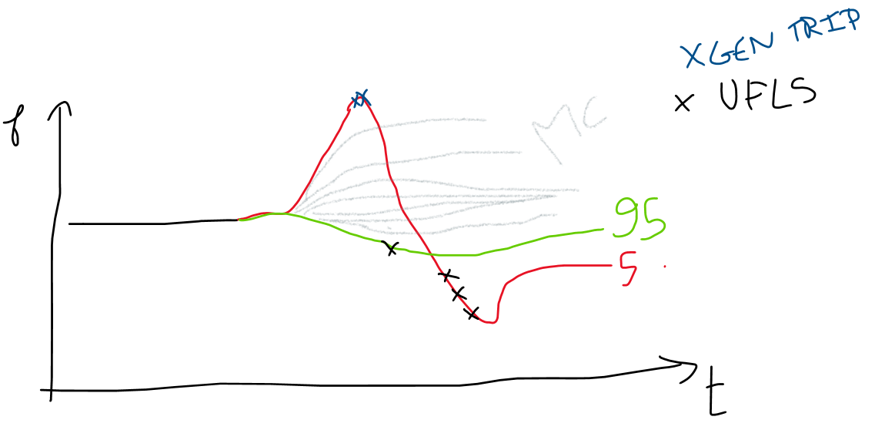
\includegraphics[width=0.8\linewidth]{Figs/isgt_frequency.png}
    \caption{Frequency evolution following the N-2 contingency of lines 7-8 and 5-8 in full T\&D simulations (dotted lines) and simulated with the dynamic equivalents (full lines)}
    \label{fig:isgt_frequency}
\end{figure}

Finally, results obtained using a netted load model are completely off which could be expected as they do not account for tripping of DERs and because simulation of large disturbances is very sensitive to modelling accuracy. It should be noted that the netted load model can both underestimate or overestimate the consequences of contingencies. For example, it predicts a full blackout for the N-2 contingency of lines 5-8 and 7-8 while more accurate models predict between 27 and 48\% of load shedding. And it predicts no consequences for the N-2 contingency of lines 16-24 and 16-21 while more accurate models predict between 15 and 55\% of load shedding.


\subsection{Conclusion}

% (Comparison of computation time quickly: core Intel Skylake 5118@2.3GHz: 2 core-hours with equivalent vs around 200 core-hours for the full TD simulations, difference would be exacerbated for larger systems. On top of the data issues). 228 init events (although in practice would probably not do 50 MC simulations)

This test case has shown that dynamic equivalents are an adequate approach to model distribution grids for the simulation of cascading outages. In particular, it has shown that building two equivalents per distribution grid (one that fits the 5th percentile of its uncertain behaviour and one that fits its 95th percentile) allows us to efficiently account for the impact of the uncertain distribution grid behaviour.

Indeed, the confidence intervals on the consequences of cascading outages are almost the same when computed using the two dynamic equivalents and when computed using MC simulations of the complete T\&D system. On the contrary, simulations performed with a netted load model lead to completely different results.



\section{Test case 2: Simulation of a real grid}
\label{sec:distrib_CIGRE}

\begin{tcolorbox}[width=\linewidth, sharp corners=all,
    colback=white!80!black,
    colframe=white!80!black]
This section is partly based on the following publication:
\begin{itemize}
    \item \fullcite{CIGRE_paper}
\end{itemize}
\end{tcolorbox}

The previous test case has shown that dynamic equivalents can adequately represent the uncertain behaviour of distribution grids during cascading outages. However, in practice, there might even more uncertainty regarding distribution networks that what has been considered in this academic test case. This second test case thus considers a real power grid and discusses how to obtain the necessary data on distribution grids.

The scope of this test case is the analysis of the impact of distribution grids on the transient stability of the Scottish transmission grid at the horizon 2022 and 2032. Section~\ref{sec:CIGRE_transmission} presents the model of the Scottish transmission grid used in this test case. Section~\ref{sec:CIGRE_distrib} then discusses the distribution model used and how the data necessary to build those models have been gathered, and section~\ref{sec:CIGRE_results} shows how distribution grids affect transient stability.

\subsection{Representative Scottish transmission grid model}
\label{sec:CIGRE_transmission}

The transmission system model considered in this study is a representative model of the GB power grid developed by Samuel Gordon in the framework of his PhD thesis~\cite{Sam_thesis}. It is based on public data and discussions with industry experts. The model provides a spatial representation of the northern part of the GB system, focusing on Scotland while aggregating the central and southern parts of England and Wales (E\&W). The point of aggregation is approx. the B7a boundary (see Figure~\ref{fig:scotland_model}) and all generation and demand south of here have been lumped in a single bus and aggregated by type (gas, HVDC, wind, etc.). The 2022 version of the model has been validated by comparing the steady-state fault levels (validating system impedances) and the stability-related boundary transfer limits (validating dynamic behaviour) to the values published by National Grid in its annual Electricity Ten Year Statement (ETYS)~\cite{ETYS}.

Samuel Gordon also developed a 2032 version of the model based on results of the 2021/22 Holistic Network Design (HND)~\cite{HND_2022}\footnote{In 2022, the ScotWind leasing round was closed and awarded 25GW of new offshore wind leasing options in Scottish waters~\cite{scotwind_2022}. This was more than many expected, and the 2021/22 HND only considered 11GW of ScotWind projects. In this model, 18.4GW have been ``piggy backed'' in the HND-proposed network~\cite{HND_2022}. A more representative model could use the recently published 2024 HND~\cite{HND_2024}.}. Compared to the 2022 version, the 2032 model has an additional 28GW of offshore wind (18 of which in Scotland), four 2GW embedded HVDC links, additional HVDC interconnectors, new and upgraded AC circuits to 400kV, 9GW of hydrogen electrolysers (4GW in Scotland), and 6.6 GW of battery storage (1.8GW in Scotland) as shown in Figure~\ref{fig:scotland_model}.

\begin{figure}
    \centering
    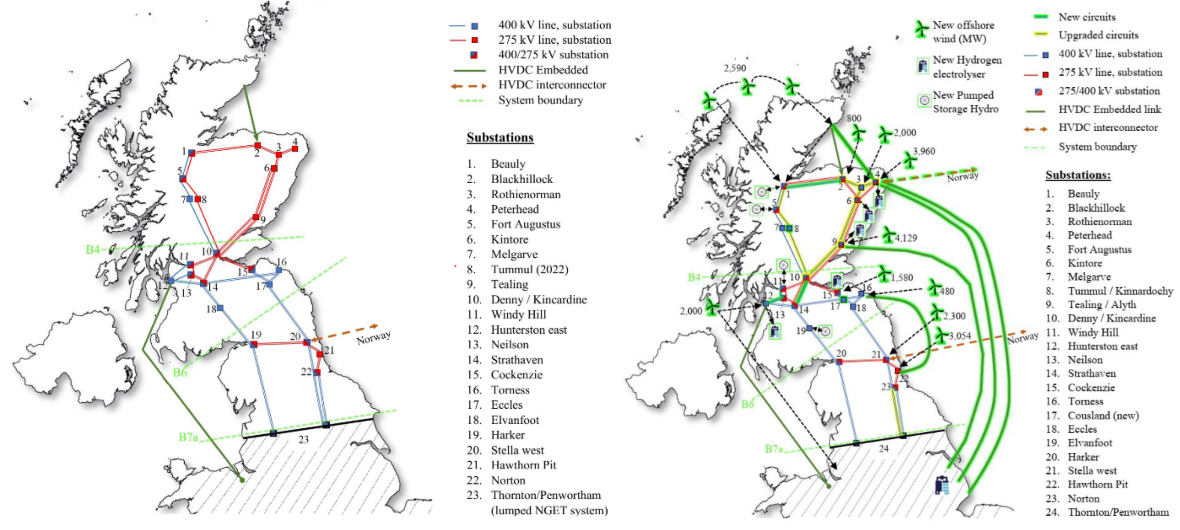
\includegraphics[width=\linewidth]{Figs/Scotland_model.pdf}
    \caption{Representative model of the Scotland power grid at the horizon 2022 (left) and 2032 (right)~\cite{Sam_thesis}}
    \label{fig:scotland_model}
\end{figure}

Scotland has a very high onshore and offshore wind potential and is thus frequently exporting power to the rest of GB. High power transfers over large distances tend to cause transient stability issues. And indeed, based on utility expertise, transient stability related transfer boundaries between Scotland and England are known to be close to thermal limits~\cite{Sam_thesis}.

To study these transient stability issues, this case study focuses on system dispatches with high power transfers from Scotland to England. Analyses have been performed for the four dispatches shown in Table~\ref{tab:scotland_dispatch}. These dispatches consider winter load peaks and summer minimum afternoon load for 2022 and 2032. The solar capacity factor (CF) for the summer afternoon cases has been set to 0.68 which correspond to the record peak high solar CF reported in~\cite{sheffield_pv}. The wind CF have been chosen in order to lead to high but realistic flows between Scotland and England.

\begin{table}
\centering
\caption{Definition of the analysed dispatches. Boundary flows in parentheses are the flows obtained before accounting for dynamic limits.}
\label{tab:scotland_dispatch}
\begin{tabular}{@{}lllllll@{}}
\toprule
Period &
    \begin{tabular}[c]{@{}l@{}}NGET\\ wind CF\end{tabular} &
    \begin{tabular}[c]{@{}l@{}}Scotland\\ wind CF\end{tabular} &
    Solar CF &
    \begin{tabular}[c]{@{}l@{}}B4 flow\\\relax [GW]\end{tabular} & % \relax to avoid use with bracket just after backslash
    \begin{tabular}[c]{@{}l@{}}B6 flow\\\relax [GW]\end{tabular} &
    \begin{tabular}[c]{@{}l@{}}Embedded HVDC\\ flow [GW]\end{tabular} \\ \midrule
Winter 2022    & 0.8 & 0.9 & 0    & 2.15 (2.75) & 2.4  & 1.69 \\
Winter 2032    & 0.8 & 0.9 & 0    & 4.02        & 2.35 & 9.41 \\
Summer PM 2022 & 0.7 & 0.7 & 0.68 & 2.28 (3.31) & 2.13 & 1.54 \\
Summer PM 2032 & 0.3 & 0.7 & 0.68 & 4.5         & 3.03 & 9.14 \\ \bottomrule
\end{tabular}
\end{table}

The system is dispatched using an optimal power flow (OPF) considering static N-1 limits. Also, as the transient stability related transfer limits through the boundaries B4 and B6 are known to be close to thermal limits, double overhead line faults have been simulated (using a netted load models\footnote{The DER production is taken as the product of the wind and solar capacity factors with the installed wind and solar DER capacities. The latter are estimated in section~\ref{sec:CIGRE_distrib_capacity}.}) for each AC circuit passing through the B4 and B6 to verify the stability of the generated dispatches. In case of instability, the OPF has been rerun with a constraint on the maximal power flow through the problematic boundary, and the maximum limit has been reduced iteratively until reaching a secure dispatch.


\subsection{Distribution system model}
\label{sec:CIGRE_distrib}

Building distribution grid models requires a significant amount of data that can be difficult to obtain. The following subsections thus describe how to how the installed DER capacities and the behaviour of those DERs have been modelled. Section~\ref{sec:CIGRE_distrib_static} then discuss the data for the other elements of distribution grids. And based on this, section~\ref{sec:CIGRE_distrib_equiv} builds full distribution models and their equivalents.

\subsubsection{Estimation of installed DER capacities}
\label{sec:CIGRE_distrib_capacity}

The installed capacities of DERs for 2022 and 2032 have been taken from the regional breakdown of the National Grid Future Energy Scenarios (FES 2022)~\cite{FES_regional}. The FES provides with estimates of gross load and installed DER capacities for every year to 2050 for four scenarios called ``Falling Short'', ``System Transformation'', ``Consumer Transformation'', and ``Leading the Way''. The ``Leading the Way'' scenario assumes significant consumer engagement and the fastest credible decarbonisation with net-zero reached in 2047. It is the only scenario considered in this study as it is expected that DERs will have the largest impact in this scenario. The FES gives estimates for every 132kV grid supply point and those have been mapped based on closest geographical distance to the 275/400kV nodes of the representative transmission model. Table~\ref{tab:der_penetration} gives the solar and wind DER penetration for each of them for the 2032 scenario.

\begin{table}
\centering
\caption{DER penetration for all load buses of the system for the 2032 scenario}
\label{tab:der_penetration}
\begin{tabular}{@{}llll@{}}
\toprule
Substation      & Peak gross load [MW] & Solar penetration (\%) & Wind penetration (\%) \\ \midrule
Peterhead       & 132                  & 49                    & 108                  \\
Stella west     & 1302                 & 35                    & 34                   \\
Hawthorn Pit    & 646                  & 42                    & 23                   \\
Harker          & 1316                 & 71                    & 42                   \\
Blackhillock    & 174                  & 84                    & 147                  \\
Cockenzie       & 931                  & 26                    & 42                   \\
Hunterston east & 507                  & 19                    & 63                   \\
Denny           & 923                  & 30                    & 38                   \\
Norton          & 1001                 & 39                    & 18                   \\
Strathaven      & 819                  & 13                    & 37                   \\
Tealing         & 472                  & 70                    & 18                   \\
Tummel          & 90                   & 51                    & 1                    \\
Windy Hill      & 938                  & 18                    & 19                   \\
Beauly          & 471                  & 24                    & 24                   \\
Kintore         & 392                  & 41                    & 43                   \\
NGET            & 53100                & 61                    & 9                    \\ \bottomrule
\end{tabular}
\end{table}

The Scotland-wide DER penetrations for solar and wind in the 2032 scenario are respectively 37\% and 36\% of the peak load. This differs significantly from the 61\% and 9\% penetration for the rest of GB. Also, two substations (Peterhead and Blackhillock), located in the North of Scotland have higher than 100\% penetration of distributed wind.



\subsubsection{DER behaviour and connection standards}

A first approach to model the behaviour of DERs is to look at the standards for DER connections. There are four main DER connection requirement standards in the UK. The relevant standard for a given installation depends on the total capacity of its inverter(s) and on the installation date as detailed in the Table~\ref{tab:UK_standards}. However, for the purpose of this analysis, there is little difference between the requirements G59, G83, and G98. Indeed, none of them have explicit low-voltage ride-through (LVRT) requirements. They do require the interface protection to disconnect the inverters if the voltage stays below 0.8pu for more than 0.5s (or 2.5s depending on the standard).  Additionally, these standards require testing to ensure that the inverter stays connected and continues to export a measurable amount of power with a voltage just above 0.8pu for at least 0.5s (depending on the standard). But there is no explicit requirement if the voltage falls below 0.8pu. This is quite similar to the situation of the 2015 Australian DER standard and AEMO (the Australian system operator) noted widespread disconnections of distributed PV following transmission faults which led them to initiate campaigns to estimate the share of inverters that disconnect for short duration voltage dips~\cite{aemo_short_duration, aemo_behaviour_2021}.

\begin{table}
\centering
\caption{Applicability of UK DER connection standards}
\label{tab:UK_standards}
\begin{tabular}{@{}lll@{}}
\toprule
Name & Scope           & Installation date                     \\ \midrule
G59~\cite{G59}  & \textgreater 16A per phase & \multirow{2}{*}{Before 27 April 2019} \\
G83~\cite{G83}  & \textless 16A per phase &                                       \\
G98~\cite{G98}  & \textless 16A per phase & \multirow{2}{*}{After 27 April 2019}  \\
G99~\cite{G99}  & \textgreater 16A per phase &                                       \\ \bottomrule
\end{tabular}
\end{table}

This is the second approach to model of behaviour of DERs: performing lab tests on inverters from many manufacturers and estimating their market share to have a global view of the average DER behaviour. In this test case however, due to lack of publicly available UK- or EU-specific data, it is assumed that all legacy DERs trip instantaneously for dips lower than 0.8pu.

For new DERs that fall in the scope of G99 and have a capacity higher than 1MW, explicit LVRT requirements must be satisfied as shown in Figure~\ref{fig:LVRT_G99}. Additionally, G99 requires ``fast fault current injection'' for units larger than 1~MW. Units must start to provide reactive support for voltages below 0.9pu and provide reactive support for 100\% of the rated current (with priority on reactive current) at 0.5pu. However, in Australia, AEMO noticed a significant share of non-compliant installations including in newer and larger installations. But again, due to lack of data, here it is assumed that DERs follow barely but strictly the G99 requirements, i.e. that units never trip above the LVRT curve, but always trip below (where tripping is allowed but not requested).

\begin{figure}
    \centering
    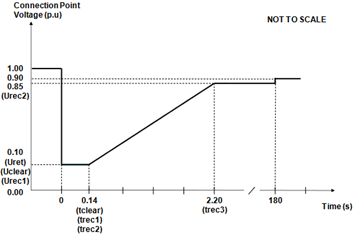
\includegraphics[width=0.7\linewidth]{Figs/G99_LVRT.png}
    \caption{LVRT requirements for inverter-based DER with a capacity between 1MW and 50MW~\cite{G99}. Inverters must stay connected for voltage dips that stay above the black line. They are allowed to stay connected or to disconnect below the black line.}
    \label{fig:G99_LVRT}
\end{figure}

Finally, DERs considered to be large generators must comply with the grid codes even if installed before 2019. The threshold is at 10MW in the north of Scotland, 30MW in the south, and 50MW in the rest of GB. The grid code (CC.6.3.15) asks for similar LVRT requirement as in G99.

Based on the above standards and requirements, DERs can be lumped into two categories. The DERs installed after 2019 with a capacity higher than 1~MW and the large generators (capacity higher than 10 to 50~MW depending on the region) are lumped as ``G99 DER'', with strict LVRT requirements and dynamic voltage support. And the remaining DERs are lumped as ``legacy DER'' without LVRT requirements no dynamic voltage support. The share of ``G99 DER'' and ``legacy DER'' is estimated by comparing the installed capacities in 2019 (from the 2019 FES data) to the ones in the study year (from the 2022 FES data). And by estimating the share of large generators from the embedded capacity register of the DSOs. All distributed large generators in Scotland are wind farms, they account for 73\% of distributed wind in the north of Scotland, 43\% in the south, and 29\% in the northeast of England~\cite{capacity_register_northern_powergrid, capacity_register_ssen, capacity_register_sp}.

All DERs are modelled using the WECC der\_a model. The tripping characteristic has however been modified to match UK standards, i.e. legacy DERs trip for voltages below 0.8pu, and G99 DERs satisfy the LVRT requirements shown in Figure~\ref{fig:G99_LVRT}.

\subsubsection{Static data and motor models}
\label{sec:CIGRE_distrib_static}

In the test case 1 and in the literature (e.g. \cite{ChaspierrePaper, ChaspierreThesis, Vorwerk}), it is assumed that the static data regarding distribution grids (line impedances, resistances, etc.) is available, and the full distribution models are thus based on these data. However, this requires many data exchanges between DSOs and TSOs and to build different models for each load. While this is possible (DSOs in UK even publish publicly some of these data), it was found easier to simply assume that the static data is uncertain.

In this example, it is assumed that the modelled distribution grids could be any of the five ``ehv'' networks from the United Kingdom Generic Distribution System (UKGDS) collection~\cite{UKGDS}. Each of those networks represent a typical small or large, rural, semi-urban, or urban UK distribution network, starting from a 132kV grid supply point up to 33/11kV transformers. The ehv1 network is shown in Figure~\ref{fig:ehv1} As these networks do not include DERs, DERs have been added in proportion to load to match the DER penetration of each load from Table~\ref{tab:der_penetration}. The networks are of course scaled to match the total gross load of all loads in Table~\ref{tab:der_penetration}.

\begin{figure}
    \centering
    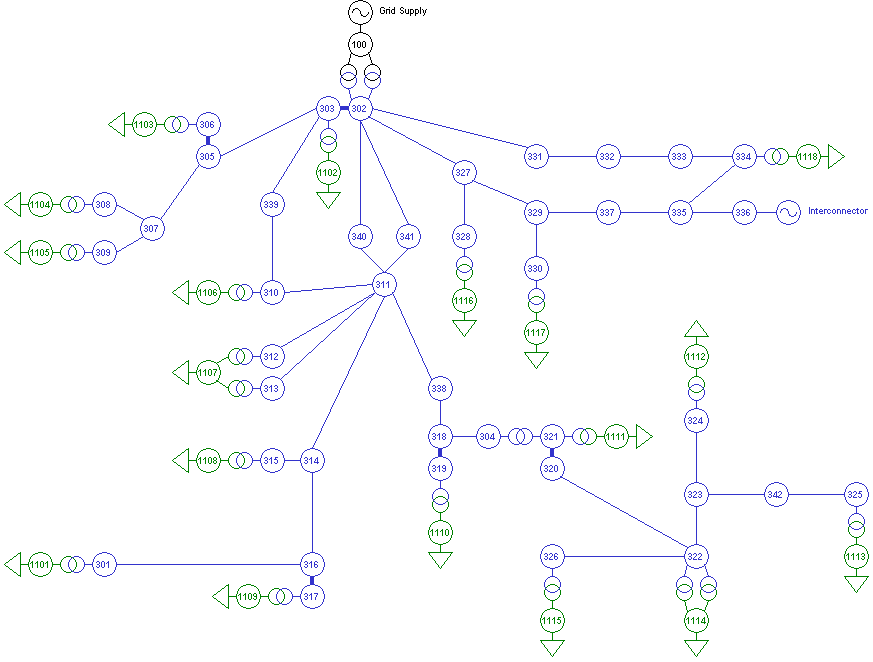
\includegraphics[width=0.8\linewidth]{Figs/ehv1.png}
    \caption{Small rural network (ehv1) from the UKGDS collection~\cite{UKGDS}}
    \label{fig:ehv1}
\end{figure}

Even if DERs play a major role in the behaviour of distribution grids, motors should not be forgotten. In this case study, motors have been modelled using WECC motor types A, B, and C. Motors D have not been considered as residential air conditioning is less prevalent in Scotland than in the US. Load motor shares have been roughly estimated assuming loads are 31\% industrial, 33\% commercial, and 36\% residential~\cite{UK_motor_share}, and based on rules of association available in~\cite{WECC_CLM_association}. Motor shares of 17\%, 11\%, and 6\% (total 34\%) have been assumed for motor types A, B, and C respectively. Due to lack of confidence, sensitivity cases with a total motor share of 30\% and 40\% have also been considered.

\subsubsection{Building dynamic equivalents}
\label{sec:CIGRE_distrib_equiv}

Now that data regarding the full distribution system model have been acquired, it is possible to train dynamic equivalents. As in the test case 1, this is done by first performing simulations of the full distribution models for a series of disturbances (with the same list of disturbances (Table~\ref{tab:disturbances}), and also connecting them to a small synchronous machine). Figure~\ref{fig:CIGRE_equiv} shows the uncertain behaviour of the full distribution model for a fault leading to a voltage dip to 0.2pu at the grid supply point lasting for 100ms. Multiple curves account for the  several UKGDS networks and the uncertain motor share.

\begin{figure}
    \centering
    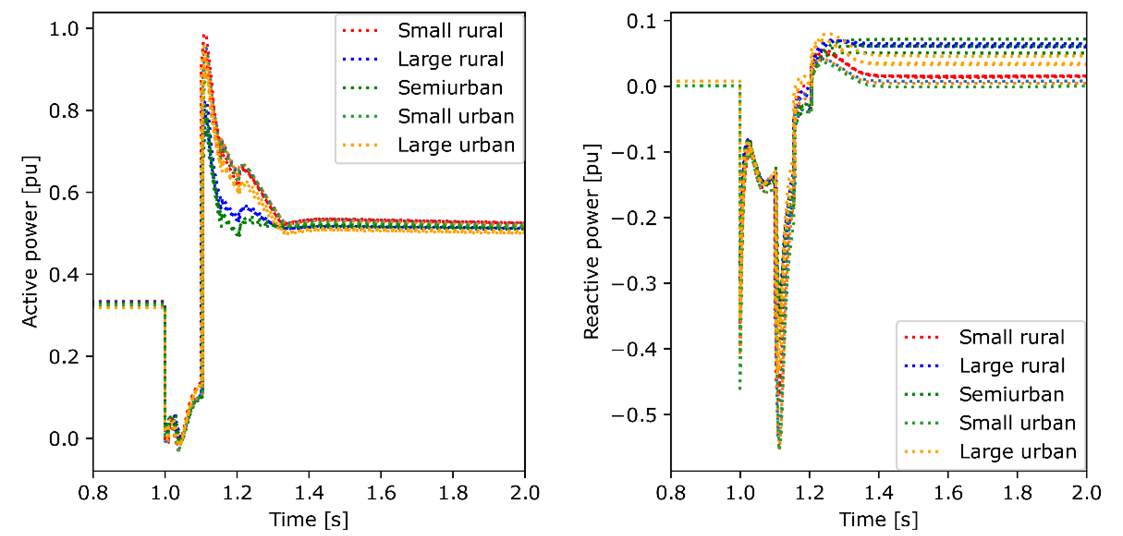
\includegraphics[width=\linewidth]{Figs/CIGRE_equiv.png}
    \caption{Active and reactive power consumption of a load for a voltage dip to 0.2pu lasting 100ms at the grid supply point. Case of Harker for the summer PM 2032 scenario, i.e. gross load = 0.93pu, installed DER capacity = 0.99pu, capacity factor = 61\%, and legacy share = 38\%. Sensitivities with a motor share of 30, 34, and 40\% are shown on the same plot.}
    \label{fig:CIGRE_equiv}
\end{figure}

\TODO{Increase figure quality}

The figure illustrates a typical behaviour for a case with a large share of G99-compliant DERs. G99 DERs do provide significant reactive support after fault clearing (from 1.1 to 1.2s on the figure), but they reduce their active power production during this time due to current limitations. There is thus a large increase in net active power consumed by the ADN after fault clearing. Also, legacy DERs trip due to the fault leading to a net increase of the steady-state active power demand.

The distribution grids behave slightly differently depending on the assumed network topology. In particular, the large rural and semi-urban networks experience a smaller active power demand peak after fault clearing. This is because those networks have a large equivalent impedance. Therefore, when DERs are providing voltage support, the distribution voltage becomes higher (in pu) than the transmission voltage. Those higher voltages alleviate the current limitations of DERs which allows them to provide more active power. In this case, the uncertain motor share does not seem to have a strong impact.

From Figure~\ref{fig:CIGRE_equiv}, a 5th and 95th percentile on the distribution behaviour can then be computed and be used to train two dynamic equivalents. The dynamic equivalent used in this test case consists of a single 33kV load bus with three motors (representing motor types A, B, and C), two DERs (one for legacy DERs and one for G99 DERs), and a static load. It is connected to the transmission system through an equivalent transformer. The DER models used in the equivalent are identical to the ones used in the full model, but they allow for partial tripping of the unit. The partial tripping model from~\cite{ChaspierreThesis} has been reused.


\subsection{Impact of distribution networks on transient stability}
\label{sec:CIGRE_results}

In all four considered dispatches, the most critical corridor (from a stability perspective) is on the west side of the B4 boundary (i.e. the two lines between Denny and Melgarve/Tummel). We thus focus on double overhead line faults on those lines\footnote{While one of the two lines is at 400kV and the other at 275kV (in the 2022 network), they both sit on the same towers, so a double overhead line fault is indeed credible.} cleared by opening the two lines. Table~\ref{tab:CIGRE_CCT} gives the critical clearing times (CCTs) for this contingency in all considered scenarios. Faults are applied near the Denny substation, i.e. just south of the B4 boundary. The impact of distribution grids is greater in this case because it leads to lower voltages on the importing side (i.e. the south) leading to more DER trips on this side, and thus a greater imbalance between the exporting and importing sides of the B4 boundary.

\begin{table}
\centering
\caption{Critical clearing times (in ms) for double overhead line faults on the west B4 corridor near Denny.}
\label{tab:CIGRE_CCT}
\begin{tabular}{@{}lllllll@{}}
\toprule
\multirow{2}{*}{Scenario} & \multirow{2}{*}{Simple model} & 5-equivalent & \multicolumn{4}{c}{95-equivalent}                     \\ \cmidrule(lr){3-3} \cmidrule(lr){4-7}
                            &                                 & Default & Default & No motors & P priority & No trips \\ \midrule
Winter   2022             & 150                             & 110     & 110     & 110       & 110        & 130      \\
Winter   2032             & 120                             & 70      & 50      & 70        & 60         & 100      \\
Summer   PM 2022          & 160                             & 120     & 100     & 110       & 110        & 150      \\
Summer   PM 2032          & 180                             & 150     & 130     & 130       & 150        & 160      \\ \bottomrule
\end{tabular}
\end{table}

The table compares the CCTs obtained with a simple load model and with the 5- and 95-equivalents. For the 95-equivalent (which gives more conservative results than the 5-equivalent), variations are also included to explain how the distribution grids impact system stability. In the ``no motors'' variation, the motor share of the load is represented by a constant impedance load. The CCTs computed in this variation are close to the base case showing that motors do not strongly impact transient stability. Motors are infamous for causing fault-induced delayed voltage recovery; however, the network has plenty of sources of dynamic reactive support (because the installed generation capacity (especially wind) is significantly larger than the demand), so voltages are quite stiff. Figure~\ref{fig:CIGRE_sensitivities} indeed shows that the voltage evolution is not very different in the ``default'' and ``no motor'' cases. The advantage of using ``physical'' dynamic equivalents instead of black-box models (e.g. artificial neural networks in ~\cite{Vorwerk}) is that such sensitivity analysis can easily be performed.

\begin{figure}
    \centering
    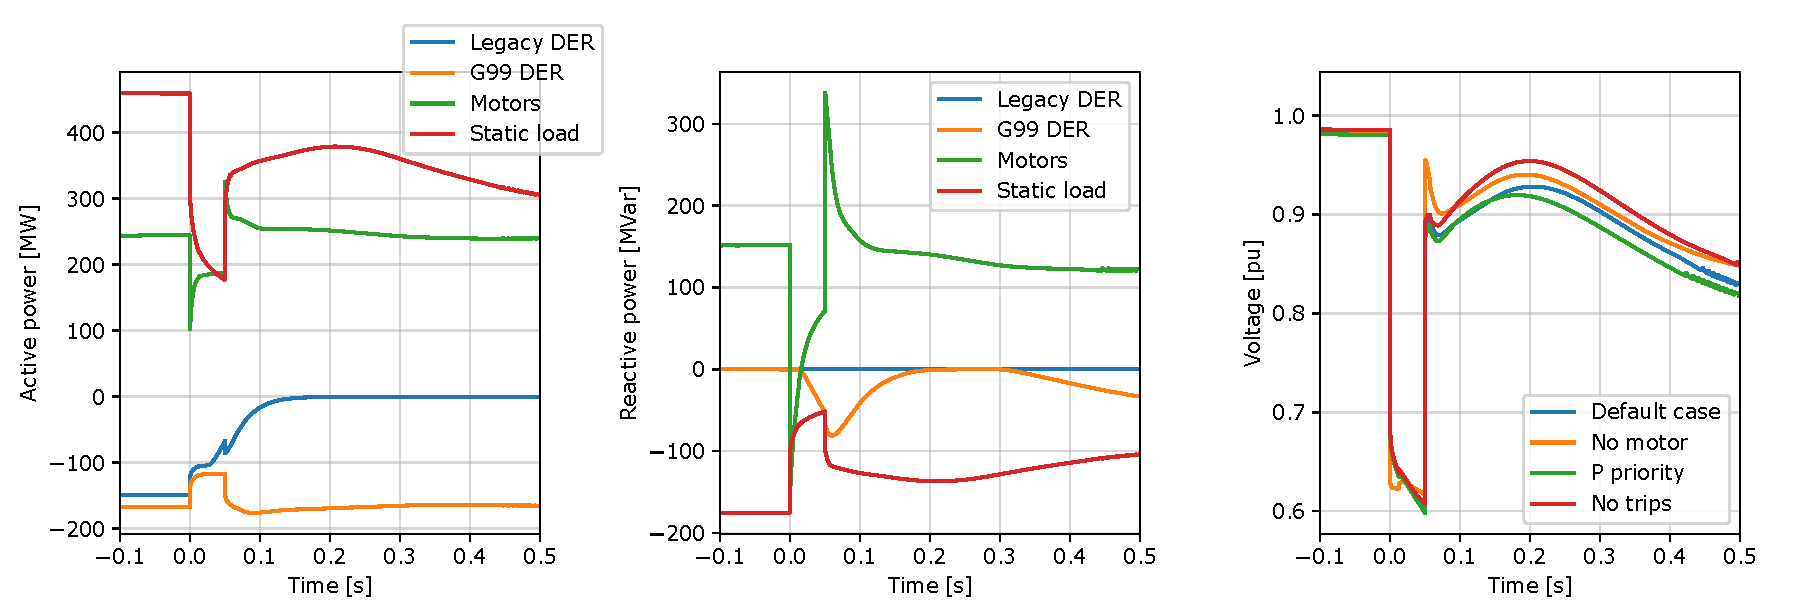
\includegraphics[width=\linewidth]{Figs/CIGRE_sensitivities.pdf}
    \caption{Behaviour of the elements of the 95-equivalent of Denny in the default case of the winter 2032 scenario for a fault cleared in critical clearing time (left and centre), and voltage at the Denny load bus in all cases (right)}
    \label{fig:CIGRE_sensitivities}
\end{figure}

Similarly, in DERs, prioritising active of reactive power only has an impact when current limits are reached, i.e. when voltage is low. In Figure~\ref{fig:CIGRE_sensitivities}, the G99 DERs provide full active power just after the fault clearing. From t=0.3s, they start to provide reactive support due to the voltage swing and thus reduce their active power production. The impact on active power production is however limited as G99 DERs only have to provide 20\% of their current capacity as reactive current at 0.8~pu voltage.

The main impact of distribution grids on system stability thus comes from the tripping of legacy DERs. In the case shown in Figure~\ref{fig:CIGRE_sensitivities} (winter 2032 scenario), 140MW of legacy DERs trip at the Denny load bus. This affects system voltages (Figure~\ref{fig:CIGRE_sensitivities} shows the voltage is highest in the no trip case) but also increases the power imbalance between the north and south of the B4 boundary. Indeed, in the winter 2032 scenario, 490MW of legacy DER trip south of B4, and almost none trip north of B4. This is because (i) the system is more meshed and transmission lines are shorter south of B4, so the fault affects more DERs in this zone, and (ii) the share of legacy DERs in larger south of B4 (more distributed PV due to the larger population and due to the smaller threshold (10 vs. 30MW) for a distributed generation to be considered large). Similar conclusion can be drawn for the other scenarios.


\subsection{Conclusion}
\label{sec:CIGRE_conclusion}

This second test case has shown that it is indeed possible to build dynamic equivalents of real distribution networks and discussed how to gather the necessary data. However, one strong assumption has been made: that DERs strictly satisfy connection requirements. A first next step of this analysis would be to validate the results based on historical disturbances. A following, more informative but more expensive test would be to perform lab tests to estimate the share of non-compliant units and to estimate how their ride through as has been done in Australia and the US~\cite{aemo_psse_2022, pourbeik_developing_2021}.

A better estimation of the (tripping) behaviour of DERs is indeed key as shown by a sensitivity analysis. Conversely, the motor share did not seem to have a large impact on simulation results. This is in part because Scotland has a lot of generation capacity with fast voltage response and a low load. But motors might impact voltage stability in the rest of GB especially near large load centres.

Finally, a second important limitation of this analysis is that inverter-based loads have not been considered. In particular, electric vehicles will account for very large shares of the load of future grids (already for the 2032 case). However, ride-through requirements for these assets still have to be defined and enforced~\cite{sygensys}.


\section{Conclusion}
\label{sec:distrib_conclusion}

This chapter has presented an approach to model distribution grids and distributed energy resources based on dynamic equivalents. The approach consists in first developing a ``full'' distribution grid model with many uncertain parameters (due to the low visibility of distribution by grids by (transmission) system operators). Then, two ``reduced'' dynamic equivalents are built: one that fits the 95th percentile of the full model and one that fits its 5th percentile. Finally, the transmission-level study of interest is performed twice: once with the 5- and once with the 95-equivalent. This allows studying the impact of distribution grid modelling uncertainties on the results of transmission studies. This is the main advantage of this approach compared to other load modelling techniques such as the component-based approach where sensitivity analyses are more difficult to perform. The proposed approach has been applied to two test cases.

In the first test case, the methodology has been used to study the impact of distribution grids on the initiating and propagation of cascading outages in an academic test grid. This test case has shown that adequately trained 5- and 95-equivalents can give confidence intervals on the consequences of cascading outages that are almost identical to the ones that would be obtained with Monte Carlo simulations of a full transmission and distribution model but are much more practical. This is important because (i) distributed energy resources are likely to trip during system disturbances and cascading outages, and (ii) because the simulation of cascading outages is quite sensitive to modelling uncertainties.

The second test case has shown that the methodology can be also be applied on real test cases with many modelling uncertainties. In particular, to limit unnecessary data exchanges between TSOs and DSOs, it was assumed that the TSO had no static data (line impedances, number of lines, etc.) regarding distribution grids. Instead, the distribution grids have been modelled using randomly selected grids from a collection of representative models of rural, semi-urban and urban distribution grids. However, the uncertain factor that has been found to affect results the most is the tripping behaviour of distributed energy resources. Indeed, connection requirements exist for distributed energy resources, but they leave margin for interpretation (can trip vs. must trip) and there are a significant share of installations that do not conform to requirements.

Future work should thus aim at better estimating the likelihood of distribution energy resources to trip following system disturbances. This can be done using measurements from past disturbances, or by performing lab tests on installations from many manufacturers. Similarly, the behaviour of inverter-based loads, and in particular, electric vehicles, should be adequately modelled as they will contribute to a large share of the load of future grids. As large-scale installation of electric vehicle chargers is just starting, this leaves room to better enforce compliance with connection requirements than for distributed energy resources.

Finally, it can be noted that in this thesis, dynamic equivalents have been built and trained independently for all loads and for all considered operating conditions. To reduce the associated computation burden, efficient updating of equivalent parameters following changes in operating conditions could be developed as proposed in~\cite{ChaspierreThesis}. Loads with similar characteristics (topology, solar penetration) could also be represented with the same equivalents.

\part{Methodological aspects of probabilistic dynamic security assessment}
\label{part:PDSA}
\chapter{Probabilistic dynamic security assessment}
\label{ch:DPSA}
\minitoc

\begin{tcolorbox}[width=\linewidth, sharp corners=all,
    colback=white!80!black,
    colframe=white!80!black]
This chapter is partly based on the following publication:
\begin{itemize}
    \item \fullcite{Journal_paper}
\end{itemize}
\end{tcolorbox}

Thanks to the previous chapters, we are now able to list the contingencies that can affect power systems, estimate their frequency of occurrence, and, for any given initial system state, estimate the potential consequences of these contingencies. The last remaining block to build a probabilistic dynamic security assessment (PDSA) methodology is the estimation of some form of probability density function (pdf) of the initial system states. Fortunately, this has been studied extensively in the literature that is reviewed in section~\ref{sec:operating_conditions}.

With all main building blocks available, it is then possible to develop a coherent PDSA methodology which is the focus of section~\ref{sec:PDSA_methodology}. This methodology is then applied to a standard test system (described in section~\ref{sec:PDSA_test_system}) in section~\ref{sec:PDSA_results}.

Probabilistic methodologies require numerous simulations which renders the interpretation of results more complex than with deterministic assessments. Some methods to interpret the results of PDSAs are thus presented in section~\ref{sec:PDSA_interpretation}. Probabilistic methodologies are intrinsically more complex than deterministic ones. To justify the need for this higher complexity, the added value of using probabilistic methods is discussed in section~\ref{sec:cascade_value}. Also, probabilistic methods require to perform many simulations which implies high computation times. The scalability of the methodology to large grids is thus discussed in section~\ref{sec:PDSA_scalability}. Finally, section~\ref{sec:PDSA_conclusion} concludes with a summary and perspectives.

\section{Operating conditions}
\label{sec:operating_conditions}

Two main methodologies have been developed in the literature to approximate the true pdf of the operating conditions of power systems.

The first methodology has initially been developed during the GARPUR (Generally Accepted Reliability Principle with Uncertainty modelling and through probabilistic Risk assessment) project~\cite{StrathElia, StrathGARPUR} and is now used by some European TSOs and by ENTSO-E to perform adequacy studies~\cite{ACER_MC_year, EliaAdequacy, ENTSOE_MC_year}. This methodology uses weather data (historical data and climate predictions) to build so-called ``Monte Carlo (MC) years''. These MC years are time-series realisations of temperature-dependent load, wind and solar availability, hydro inflows (rain, ice melting) and random availability (due to forced outages) of generating units and transmission elements. The use of weather data allows for adequate modelling of the spatio-temporal correlations between all random variables (renewable availability, load, asset availability)~\cite{StrathGARPUR, ENTSOE_MC_year}. Then, for each MC year, a market model is used to determine the commitment of thermal and hydro generators. Finally, each year is divided into (\eg hourly) snapshots and an optimal power flow (OPF) is performed to account for potential preventive actions that could be performed by operators to make the system secure. Typically, this OPF will include constraints to guarantee that static limits are not exceeded in all possible N-1 conditions. All snapshots are then saved in a database to be used in the rest of the analysis (\eg adequacy or security assessment\footnote{Depending on the type of analysis, a different level of granularity might be used. For adequacy studies, a zonal approach is typically used, while for security studies, a nodal approach is used.}).


The second methodology has been developed during the iTesla project~\cite{KonstantelosCopulas, EurostagHPC, iTesla_uncertainties}. It consists in directly fitting a multivariate pdf to the true pdf of system states using historical data. Copulas are used to model the correlations between variables. The advantage of this method compared to the GARPUR approach is that it can potentially be more accurate since it is directly based on real historical system states. In particular, the iTesla approach is especially effective at predicting the system topology (\ie substation configurations) for a given realisation of renewable availability and load. This is more difficult in the GARPUR approach as topology optimisations introduce many binary variables into OPFs which makes them difficult to solve.

However, the reliance on historical data makes the iTesla approach less flexible. In particular, it does not allow for the modelling of the impact of climate change on weather and severe weather events. This has however been done using the GARPUR approach in~\cite{ENTSOE_MC_year}. Also, if operating rules are modified (\eg to enhance security as we will discuss in section~\ref{sec:PDSA_interpretation}) or if new elements are added to the system (\eg new lines), historical data on operator actions might no longer be relevant. Finally, the iTesla approach is relatively poorly documented, so only the GARPUR approach will be considered in the test cases studied in this thesis.

When building a database of operating conditions, the database should be large enough to include a wide variety of possible system states. However, because adequacy and security studies have different objectives, databases used for security do not need to be as large as for adequacy studies (around 200 MC years for adequacy~\cite{EliaAdequacy}). Indeed, adequacy studies check that the load can be fully satisfied in most system states. A typical adequacy criterion is that the expected number of hours during which the load cannot be satisfied is lower than 3h per year (\ie 3 operating points out of 8760 if hourly snapshots are considered). The database of operating states should thus include many MC years such that the statistical accuracy of the analysis is better than 3h per year.

On the other hand, in a security study, contingencies are applied onto operating states. It can thus be said that adequacy focuses on N-0 states (where N already accounts for unavailable assets) while security focuses on N-1 and N-k contingencies. Because contingencies have a relatively low frequency of occurrence (around 1 per year for N-1 contingencies and lower for higher order contingencies, compared to the N-0 state that continuously occur), a contingency that only has consequences for states that occur 3h per year (0.3\% of the time) will have a very low contribution to the risk\footnote{Table~\ref{tab:critical_contingencies} shows that contingencies with a high contribution to the risk typically have non-zero consequences for 5 to 50\% of operating conditions. However, this table only accounts for N-2 contingencies and delayed-clearing N-1 contingencies, so this figure could be lower for N-1 contingencies with normal clearing time.}. In any case, building a large database is computationally inexpensive (compared to performing thousands of dynamic simulations), so an arbitrarily large database of operating conditions can theoretically be generated.


\section{Security assessment methodology}
\label{sec:PDSA_methodology}

Now that all building blocks are available, a PDSA methodology can be developed. The methodology proposed in this thesis consists of three main steps as shown in the flowchart in Figure~\ref{fig:flowchart}. The first step is the generation of a large database of likely system states for which security will be assessed. In this thesis, this step is implemented using the GARPUR approach presented in section~\ref{sec:operating_conditions}. Although in theory, any technique that can generate system dispatches that follow the pdf of system states can be used.



\begin{figure}
\centering
% Flowchart template based on Brent Longborough, "Flowcharting techniques for easy maintenance"
\begin{tikzpicture}[%
    >=triangle 60,              % Nice arrows; your taste may be different
    start chain=going below,    % General flow is top-to-bottom
    node distance=5mm and 25mm, % Global setup of box spacing
    every join/.style={norm},   % Default linetype for connecting boxes
    font=\small,
    ]
% -------------------------------------------------
% A few box styles
% <on chain> *and* <on grid> reduce the need for manual relative
% positioning of nodes
\tikzset{
base/.style={draw, on chain, on grid, align=center, minimum height=4ex},
proc/.style={base, rectangle, text width=12em},
shortproc/.style={base, rectangle, text width=9em},
test/.style={base, diamond, aspect=2, text width=4em},
term/.style={proc, rounded corners},
storage/.style={base, ellipse, text width=8em},
% coord node style is used for placing corners of connecting lines
coord/.style={coordinate, on chain, on grid, node distance=6mm and 25mm},
% nmark node style is used for coordinate debugging marks
nmark/.style={draw, cyan, circle, font={\sffamily\bfseries}},
% -------------------------------------------------
% Connector line styles for different parts of the diagram
norm/.style={->, draw},
}
% -------------------------------------------------
% Start by placing the nodes
\node [proc] (market) {Sample renewable availability and load};
% Use join to connect a node to the previous one
\node [proc, join]  (dispatch)    {Dispatch the system};
\node [storage, join] (database) {Operating conditions database};


% \node [proc, below=20mm of database] (start) {Set \parbox{1cm}{\(i=1\)}};  % parbox because otherwise uses very wide spacing around =
% \node [proc, join]   (contingency)   {Select contingency \(i\)};
\node [proc, below=25mm of database] (conditions) {Select contingency and sample operating conditions};
\node [test, join] (screen) {Screen scenario};

\node [shortproc, below left=18mm and 22mm of screen] (simulation) {Simulate contingency and evaluate consequences};
\node [shortproc, below right=18mm and 22mm of screen] (safe) {Set consequences to 0};

\node [test, below=40mm of screen]   (accuracy_reached)   {Statistical accuracy reached?};
% \node [test, join] (i_max) {\(i < i_{max}\)};
% \path (i_max.east) to node [near start, yshift=1em, xshift=1.5em] {\(i = i + 1\)} (i_max);

\node [proc, join, below=28mm of accuracy_reached]   (critical)   {Compute risk and identify critical contingencies};
\node [proc, join]   (ML)   {Define ML-based operating rules to secure critical contingencies};

% More complex annotations
\node [coord, left=of screen] (t1left)  {};
\path (screen.west) to node [near start, yshift=2em, xshift=-2em] {Unsecure} (simulation);
\draw [->] (screen.west) -| (simulation.north);
\path (screen.east) to node [near start, yshift=2em, xshift=2em] {Secure} (safe);
\draw [->] (screen.east) -| (safe);

\draw [->] (simulation) -- (accuracy_reached);
\draw [->] (safe) -- (accuracy_reached);

\node [coord, right=41.5mm of accuracy_reached] (c2)  {};
\draw [->] (accuracy_reached.east) -- (c2) |- ([yshift=-2mm] conditions);
% \node [coord, right=43mm of i_max] (c3)  {};
% \draw [->] (i_max.east) -- (c3) |- (contingency);
\node [coord, right=50mm of ML] (c5)  {};
\draw [->] (ML.east) -- (c5) |- (dispatch);
\node [coord, right=30mm of database] (c1)  {};
\draw [->, dashed] (database.east) -- (c1) |- ([yshift=2mm] conditions);


% Background boxes
\node [above left=4mm and 18mm of market, anchor=west] (label1) {\parbox{6cm}{Operating condition database generation}};
\node [above left=4mm and 18mm of conditions, anchor=west] (label2) {\parbox{6cm}{Security assessment}};
\node [above left=4mm and 18mm of critical, anchor=west] (label3) {\parbox{6cm}{Security enhancement}};

\coordinate[right=21mm of market] (aux1);
\coordinate[right=21mm of conditions] (aux2);
\coordinate[right=21mm of critical] (aux3);

\begin{scope}[on background layer]
    \node[fill=yellow!15,fit=(label1) (aux1) (market) (dispatch) (database)]{};
    \node[fill=green!15,fit=(label2) (aux2) (conditions) (screen) (simulation) (safe) (accuracy_reached)]{};
    \node[fill=red!15,fit=(label3) (aux3) (critical) (ML)]{}; % draw,dashed,gray,rounded corners
\end{scope}

\end{tikzpicture}
\caption{Flowchart of the proposed PDSA methodology}
\label{fig:flowchart}
\end{figure}

% \begin{figure}
% \centering
% % Flowchart template based on Brent Longborough, "Flowcharting techniques for easy maintenance"
% \begin{tikzpicture}[%
%     >=triangle 60,              % Nice arrows; your taste may be different
%     start chain=going below,    % General flow is top-to-bottom
%     node distance=5mm and 25mm, % Global setup of box spacing
%     every join/.style={norm},   % Default linetype for connecting boxes
%     font=\small,
%     ]
% % -------------------------------------------------
% % A few box styles
% % <on chain> *and* <on grid> reduce the need for manual relative
% % positioning of nodes
% \tikzset{
% base/.style={draw, on chain, on grid, align=center, minimum height=4ex},
% proc/.style={base, rectangle, text width=12em},
% shortproc/.style={base, rectangle, text width=9em},
% test/.style={base, diamond, aspect=2, text width=4em},
% term/.style={proc, rounded corners},
% storage/.style={base, ellipse, text width=8em},
% % coord node style is used for placing corners of connecting lines
% coord/.style={coordinate, on chain, on grid, node distance=6mm and 25mm},
% % nmark node style is used for coordinate debugging marks
% nmark/.style={draw, cyan, circle, font={\sffamily\bfseries}},
% % -------------------------------------------------
% % Connector line styles for different parts of the diagram
% norm/.style={->, draw},
% }
% % -------------------------------------------------
% % Start by placing the nodes
% \node [proc] (market) {Sample renewable availability and load};
% % Use join to connect a node to the previous one
% \node [proc, join]  (dispatch)    {Dispatch the system};
% \node [storage, join] (database) {Operating conditions database};
%
%
% % \node [proc, below=25mm of database] (start) {Set \parbox{1cm}{\(i=1\)}};  % parbox because otherwise uses very wide spacing around =
% \node [proc, below=25mm of database] (contingency) {Select contingency \(i\)};
% \node [proc, join] (conditions) {Sample operating conditions};
% \node [test, join] (screen) {Screen scenario};
%
% \node [shortproc, below left=18mm and 22mm of screen] (simulation) {Simulate contingency and evaluate consequences};
% \node [shortproc, below right=18mm and 22mm of screen] (safe) {Set consequences to 0};
%
% \node [test, below=40mm of screen]   (accuracy_reached)   {Statistical accuracy reached?};
% \node [test, join] (i_max) {\(i < i_{max}\)};
% \path (i_max.east) to node [near start, yshift=1em, xshift=1.5em] {\(i = i + 1\)} (i_max);
%
% \node [proc, join, below=28mm of i_max]   (critical)   {Compute risk and identify critical contingencies};
% \node [proc, join]   (ML)   {Define ML-based operating rules to secure critical contingencies};
%
% % More complex annotations
% \node [coord, left=of screen] (t1left)  {};
% \path (screen.west) to node [near start, yshift=2em, xshift=-2em] {Unsecure} (simulation);
% \draw [->] (screen.west) -| (simulation.north);
% \path (screen.east) to node [near start, yshift=2em, xshift=2em] {Secure} (safe);
% \draw [->] (screen.east) -| (safe);
%
% \draw [->] (simulation) -- (accuracy_reached);
% \draw [->] (safe) -- (accuracy_reached);
%
% \node [coord, right=41.5mm of accuracy_reached] (c2)  {};
% \draw [->] (accuracy_reached.east) -- (c2) |- ([yshift=-2mm] conditions);
% \node [coord, right=43mm of i_max] (c3)  {};
% \draw [->] (i_max.east) -- (c3) |- (contingency);
% \node [coord, right=50mm of ML] (c5)  {};
% \draw [->] (ML.east) -- (c5) |- (dispatch);
% \node [coord, right=30mm of database] (c1)  {};
% \draw [->, dashed] (database.east) -- (c1) |- ([yshift=2mm] conditions);
%
%
% % Background boxes
% \node [above left=4mm and 18mm of market, anchor=west] (label1) {\parbox{6cm}{Operating condition database generation}};
% \node [above left=4mm and 18mm of contingency, anchor=west] (label2) {\parbox{6cm}{Security assessment}};
% \node [above left=4mm and 18mm of critical, anchor=west] (label3) {\parbox{6cm}{Security enhancement}};
%
% \coordinate[right=21mm of market] (aux1);
% \coordinate[right=21mm of conditions] (aux2);
% \coordinate[right=21mm of critical] (aux3);
%
% \begin{scope}[on background layer]
%     \node[fill=yellow!15,fit=(label1) (aux1) (market) (dispatch) (database)]{};
%     \node[fill=green!15,fit=(label2) (aux2) (conditions) (screen) (simulation) (safe) (accuracy_reached) (i_max)]{};
%     \node[fill=red!15,fit=(label3) (aux3) (critical) (ML)]{}; % draw,dashed,gray,rounded corners
% \end{scope}
%
% \end{tikzpicture}
% \caption{Flowchart of the proposed PDSA methodology}
% \label{fig:flowchart}
% \end{figure}


The second step is the security assessment itself. In this step, initial operating conditions are sampled from the database generated in the previous step and contingencies are applied to these initial states. Time-domain simulations are then used to determine if those contingencies are secure or if they can lead to cascading outages. In the latter case, time-domain simulations are also used to evaluate the potential consequences of these cascades.

However, as discussed previously, cascading outages are difficult to simulate as their evolution can be very sensitive to the timing of protection system operations. For each sampled scenario (combination of a contingency and initial state), the indicator developed in section~\ref{sec:protection_uncertainty} is used to determine if the scenario is sensitive to protection-related uncertainty. If it is, MC simulations of the scenario are performed to assess the impact of protection-related uncertainties on this scenario. If it is not, a single simulation is enough. The sampling of protection-related uncertainties will be discussed in more details in section~\ref{sec:PDSA_results_protections}.

The main question when doing MC simulations is how to efficiently sample and when to stop sampling. This is discussed in section~\ref{sec:sampling}. To limit computation time, scenarios which are expected to be secure can be screened out of the analysis. The stability indicators used for this purpose are described in section~\ref{sec:screening}. However, even with the above points, performing a PDSA requires a significant amount of computation time. Fortunately, it is straightforward to parallelise as different scenarios can be simulated independently on different computer cores. The implementation of the proposed methodology in a high-performance computing (HPC) environment is thus discussed in section~\ref{sec:HPC} and applied in section~\ref{sec:PDSA_results} on the test system presented in section~\ref{sec:PDSA_test_system}.

Finally, the third step consists in interpreting the results of the security assessment and in using them to enhance the security of the system (\ie to reduce the risk of unwanted load shedding) as a first step towards probabilistic security \emph{management}. This is discussed in section~\ref{sec:PDSA_interpretation}.


\subsection{Sampling operating conditions and stopping criteria}
\label{sec:sampling}

Once a database of initial system states is generated (based on section~\ref{sec:operating_conditions}), contingencies can be applied to those states to perform the security assessment. However, systematically simulating all combination of contingencies and system states would be extremely time-consuming and wasteful.

In the GARPUR approach, system states in the generated database are first clustered, and then the analysis is performed on the cluster centroids, reducing the number of scenarios to simulate. The issue with this approach is that the number of clusters has to be defined before performing the analysis (at least with the clustering technique (K-means) used in GARPUR). Moreover, it is very difficult to quantify the error introduced by the clustering process, and thus to strike a good balance between the number of clusters and computation time. Finally, clustering is difficult to use with high-dimensional data because it is rare for any two points to be ``close'' from each other in a high-dimensional space.

Indeed, Table~\ref{tab:clustering} shows that when clustering operating points from one year of operation of the RTS-GMLC system (test system described in section~\ref{sec:PDSA_test_system}), most clusters consist in a single point if the maximum distance between close points is set to 50~MVA. In this case, the distance between two operating points is defined as the infinity norm distance between the vectors of active and reactive power flows in all generators and transmission elements. In other words, the distance between the point \(j\) and \(k\) is computed as

\begin{equation}
% \begin{split}
d^{\infty}_{jk} = \max{\left[\max_g{\left(\abs{P_{g, j} - P_{g, k}}, \abs{Q_{g, j} - Q_{g, k}}\right)}, \max_b{\left(\abs{P_{b, j} - P_{b, k}}, \abs{Q_{b, j} - Q_{b, k}}\right)}\right]}
% \end{split}
\end{equation}

\noindent where \(P_{g, j}\) is the active power output of generator \(g\) in the dispatch \(j\) and \(P_{b, k}\) is the power flow in branch \(b\) in the dispatch \(k\). So a distance higher than 50~MVA implies that the active or reactive flow in at least one line and/or the active or reactive production of at least generator differs by more than 50~MW or 50~MVAr between two given dispatches. Almost all generators and branches have a rating lower or equal than 500~MW, so a distance of 100~MW is already non-negligible. However, clustering with a maximum distance of 100~MW still leads to 2752 clusters which would be computationally expensive to all simulate for all contingencies.

\begin{table}
\centering
\caption{Grouping of 8617 initial states of the RTS-GMLC into clusters with a maximum intra-cluster infinity norm distance}
\label{tab:clustering}
\begin{tabular}{@{}lll@{}}
\toprule
Distance [MVA] & \# clusters & \# points per cluster \\ \midrule
5             & 8612        & 1.0006    \\
10            & 8580        & 1.004     \\
20            & 8340        & 1.03      \\
50            & 5916        & 1.46      \\
100           & 2752        & 3.13      \\
200           & 989         & 8.71      \\ \bottomrule
\end{tabular}
\end{table}

Instead, in this thesis, the system states are sampled using MC techniques. As for any MC algorithm, the main question is how to efficiently sample and how many samples to simulate to reach a target statistical accuracy with minimal computation burden.

% TODO: better stopping criteria (or ref to a later discussion) + talk more about risk of individual contingencies (important point of methodology but not discussed in details). Potentially mention groups of contingencies (would need to be defined in advance, if ok for individual, ok for total, but reduces coverage part)

The standard MC approach is to sample system states proportionally to their likelihood until a stopping criterion is reached. Most papers stop sampling once they obtain satisfactory accuracy on the \emph{total} risk estimate. This thesis however argues that it is more useful to have an accurate estimation of the risk from the main risk contributors, and in particular, an estimation of the risk of \emph{individual} contingencies. Indeed, most security-enhancement actions (synchronous condensers, redispatches, system integrity protection schemes) solve local issues caused by a limited set of contingencies. To efficiently reduce the total risk, it is thus necessary to identify the most critical contingencies and to focus on reducing their individual contributions to the risk. Therefore, a stopping criterion is defined for each contingency\footnote{It would also be possible to instead define a stopping criterion based on the risk associated with groups of contingencies or on the risk associated with a given protection system, for example, if the goal of the analysis is to quantify the effectiveness of a given risk-mitigation action. However, this would mean that the analyst would no longer be able to decompose the total risk (or risk associated with a group of contingencies in this example) into individual risk contributions which would make the interpretation of the results more difficult.} as

\begin{equation}
  \label{eq:stop}
  SE_i \leq \epsilon \; R
\end{equation}

\noindent where \(SE_i\) is the standard error (SE) of the risk estimate of contingency \(i\), \(R\) is the total estimated risk (from all contingencies), and \(\epsilon\) is a user-defined threshold. System states are thus sampled independently for each contingency until the SE of each contingency is smaller than a fraction of the total risk (\(\epsilon \, R\)). To be clear, all contingencies (up to a given order) are enumerated (not sampled), and system states are sampled. Equation (\ref{eq:stop}) guarantees (with some level of confidence) that the most critical contingencies are correctly identified (if their contribution to the total risk is higher than \(\epsilon \, R\)). The choice of an adequate value for \(\epsilon\) is better discussed through an example and is thus discussed in section~\ref{sec:PDSA_results_sampling} and Figure~\ref{fig:SE_individual}.

The above criterion requires an estimate of the total risk. Thus, to warm up the algorithm, simulations are performed for all contingencies and for a few (\eg 5) operating conditions samples. This gives a first (rough) estimate of the total risk. Contingencies for which the stopping criterion (\ref{eq:stop}) is far from being satisfied are then sampled with higher priority. The estimate of the total risk is iteratively improved when more samples are simulated until (\ref{eq:stop}) is satisfied for all contingencies.

When using the standard MC approach, the SE can be computed as

\begin{equation}
  \label{eq:SE_classic}
  SE_i = f_i \sqrt{\frac{\sigma_i^2}{N_i}}
\end{equation}

\noindent where \(f_i\) is the frequency of contingency \(i\) and \(\sigma_i^2\) is the variance of its consequences. However, this variance is often unknown and therefore approximated by the sample variance \(\tilde{\sigma}_i^2\).

This approximation is commonly used but can be inaccurate especially for contingencies whose consequences strongly depend on the operating conditions and for small values of \(N_i\). For example, if \(N_i\) samples of operating conditions are drawn for a given contingency and all show no consequences, the sampled variance will be zero, therefore the stopping criteria will be satisfied, and no other samples will be drawn. In this case, the confidence interval \([\tilde{\mu_i} - x SE_i, \tilde{\mu_i} + x SE_i]\) (where \(\tilde{\mu_i}\) are the sampled average consequences of contingency \(i\)) is infinitely narrow regardless of the value of \(x\) indicating perfect statistical accuracy. However, the \(N_i+1\)th sample might still lead to a blackout showing that the above approach might underestimate the risk.

To estimate the bias introduced in the above approach, it is useful to notice that if a contingency has a probability \(p_i\) to have consequences, the probability for \(N_i\) out of \(N_i\) samples to show no consequences is \((1-p_i)^{N_i}\). Conversely, if \(N_i\) out of \(N_i\) samples show no consequences, then \(p_i\) satisfies

\begin{equation} \label{eq:proba}
  p_i < 1 - \sqrt[N_i]{1-\alpha} \ \text{with}\ \alpha \ \text{confidence}
\end{equation}

In this case, an upper bound on the bias is \(f_i p_i M_C\) where \(M_C\) are the maximum consequences of a contingency (\eg a complete blackout). When \(N_i\) is large, equation (\ref{eq:proba}) can be approximated using a first-order Taylor expansion as

\begin{equation} \label{eq:proba_approx}
  p_i < \frac{|\ln(1-\alpha)|}{N_i}
\end{equation}

% proof of 1-0.05^1/N_i = 3/N_i: Taylor: a^x = 1 + [a^x ln(a)]_0 * x = ln(0.05) * x =  2.99573*x

In the more general case, where a non-zero number of samples (out of \(N_i\)) lead to consequences, the true mean \(\mu_i\) and variance \(\sigma_i\) of the consequences \(c_i\) of contingency \(i\) can be bounded by the sampled mean and variance of

\begin{equation}
  C_i = (1-p_i) \tilde{c_i} + p_i M_C
\end{equation}

\noindent where \(\tilde{c_i}\) is the sampled pdf of \(c_i\) and \(p_i M_C\) accounts for potential unsecure regions missed in the sampled \(\tilde{c_i}\). The following bounds can thus be obtained


\begin{IEEEeqnarray}{rCl}
  \mu_i & \leq & (1-p_i) \tilde{\mu_i} + p_i M_C \\
  \sigma_i^2 & \leq & (1-p_i) \tilde{\sigma_i^2} + p_i \beta_i^2 \ \text{where} \ \beta_i^2 = (M_C - \tilde{\mu_i})^2 \label{eq:sigma_bound}
\end{IEEEeqnarray}

Considering that, for large \(N_i\), \((1-p_i) \approx 1\) and injecting (\ref{eq:proba_approx}) and (\ref{eq:sigma_bound}) in (\ref{eq:SE_classic}), the following bound can be obtained for the SE of the risk of contingency \(i\)

\begin{equation}
  SE_i \leq f_i \sqrt{\frac{\tilde{\sigma}_i^2}{N_i} + \frac{|\ln(1-\alpha)| \beta_i^2}{N_i^2}}
\end{equation}

\noindent which, for \(\alpha = 95\%\), becomes

\begin{equation}
  \label{eq:SE_bound}
  SE_i \leq f_i \sqrt{\frac{\tilde{\sigma}_i^2}{N_i} + \frac{3 \beta_i^2}{N_i^2}}
\end{equation}

% \begin{equation}
%   SE_i \leq f_i \sqrt{(1-p_i) \frac{\tilde{\sigma^2}}{N} + p_i \frac{\beta_i}{N}} \approx f_i \sqrt{\frac{\tilde{\sigma^2}}{N} + \frac{3 \beta_i}{N^2}}
% \end{equation}

This bound can then be used in the stopping criteria (\ref{eq:stop}). The first term in this bound is the classical variance term, and the second term represents how good is the ``coverage'' of the MC sampling, \ie how (un)likely it is to have missed important scenarios in the sampling process.


The derivation above has been made for the case of a crude MC estimator (\ie sampling of system states based on their likelihood). Crude MC estimators can be slow to converge, especially in the presence of low frequency high impact scenarios, and more sophisticated methods have thus been developed. In the field of power systems, a commonly used method is importance sampling. It usually consists in biasing the sampling process towards unsecure cases in order to have more samples with consequences. In the context of resilience, this can be done for example by sampling more frequently the more severe earthquakes, because small earthquakes, while more frequent, will have a lower contribution to the risk as they often have low consequences.

In the context of security assessment, importance sampling is more difficult to use because it is difficult to know a priori if a given contingency will be less secure in the cases with high wind, the cases with high solar, and/or the cases with high/low load, etc. Adaptive importance sampling methods such as cross-entropy importance sampling circumvent this issue by drawing a first batch of samples in a crude MC way, identifying unsecure zones, then iteratively drawing additional batches of samples biased towards the unsecure zones. This approach can be dangerous because if an unsecure region is missed in the first batch, it will be increasingly more unlikely to be discovered it in the following batches.

Indeed, importance sampling (and other variance-reduction techniques) aim to reduce the variance of the MC estimator, but do not necessarily give better coverage. Actually, if the security region of a given contingency is not know a priori, crude MC is the most efficient sampling approach to minimise the risk associated with missed scenarios. Therefore, variance-reduction techniques can only be useful if

\begin{equation}
  \label{eq:coverage_requirement}
  \frac{\tilde{\sigma_i^2}}{N_i} > \frac{3 \beta_i^2}{N_i^2}
\end{equation}

However, as will be shown in the application in section~\ref{sec:PDSA_results_sampling} (notably in Fig.~\ref{fig:indic_N1} and \ref{fig:indic_N2}), the coverage term is often dominant for most contingencies, and a crude MC sampling of operating conditions is therefore the most effective approach.

Similarly, ML models could be trained using a first batch of MC simulations, and then used to speed up the simulation of the following MC samples. But again, if an unsecure zone is missed in the first batch, the ML model will not be able to predict it. So the criterion~(\ref{eq:coverage_requirement}) should also be satisfied before applying data-driven methods to speed up the MC simulation.



\subsection{Screening}
\label{sec:screening}

The section above just stated that crude MC sampling is the most efficient approach to guarantee adequate coverage of the sampling space for PDSA (at least for most contingencies). Because power systems are operated with a high level of reliability, a high share of MC simulations might be for secure and thus ``uninteresting'' scenarios. For example, the test system considered that will be considered in section~\ref{sec:PDSA_results} is operated according to the classical N-1 criterion, yet more than 90\% of the considered N-2 scenarios (failure of 2 adjacent branches due to breaker failure to open following a line fault) do not lead to consequences.

This indicates that a significant speed-up can be obtained if secure scenarios are screened out of the analysis (up to a factor 10 in this case). As this thesis focuses on dynamic stability, the security of any scenario is predicted using three stability indicators, one for each of the main instability types: angle, voltage, and frequency. If long-term stability is of interest, additional indicators should be used. The stability indicators used in this thesis are as follows.

For angle stability, the critical clearing time (CCT) is estimated via the extended equal area (EEA) method~\cite{EqualAreaCriterionEnergies} (using the critical cluster evaluation method from~\cite{EqualAreaCriterionPSCC}). A scenario is deemed unsecure if the actual clearing time is larger than the estimated CCT plus a 50ms margin. The 50ms margin is used because it is preferable to have false positives (\ie secure scenarios that are predicted to be unsecure) rather than false negatives (\ie unsecure scenarios predicted secure). Indeed, for false positives, unnecessary simulations will be performed which increases computation time but do not affect the risk estimate (because simulations of false positives will simply show that they are secure), while false negatives cause to underestimate the risk (because unsecure scenarios are disregarded).

The EEA method concerns the stability of synchronous generators. Some papers (\eg~\cite{ScreeningPLL}) argue that inverter-based generators can be modelled as synchronous machines with an inertia \(\frac{1}{K_i}\) where \(K_i\) is the gain of the integral component of the PLL. However, due to the large (\(>10\)s\textsuperscript{-1}) gains typically used, this leads to very low CCTs. However, this does not account for fault-ride through modes of inverters. In this thesis, inverter-based generators are thus modelled as constant-impedance negative loads for the purpose of EEA.

For voltage stability, the indicator from~\cite{VoltageScreeningMachowski} is used, \ie a scenario is considered voltage secure if the short-circuit power at all buses (after the occurrence of the contingency) is larger than 4 times the apparent power of the load of the bus. Regarding frequency stability, based on preliminary simulations on the RTS-GMLC, a scenario is deemed secure if it leads to a rate of change of frequency lower than 0.4~Hz/s and a loss of power generation less than 70\% of the primary reserve. Generators near a fault are assumed to be disconnected (in the computation of the screening indicators) if the fault lasts longer than 150ms. The RoCoF is estimated via

\begin{equation}
\text{RoCoF} = \frac{\Delta P}{2 H}
\end{equation}

\noindent where \(\Delta P\) is the load generation imbalance directly following the loss of a generator or islanding, and \(H\) is the inertia of the system.


\subsection{Implementation in an HPC environment}
\label{sec:HPC}

The method described above can be implemented in an HPC environment using a master-slave architecture similar to the one used in~\cite{EurostagHPC}. The master node is responsible for scheduling the simulations to be performed, and the slaves nodes are responsible for performing those simulations and sending the results back to the master node.

A typical run goes as follows. First, the master schedules all contingencies to be simulated for a small number (\eg 5) of random operating conditions. This warm-up step allows the master to evaluate the stopping criterion~(\ref{eq:stop}) and to compute a first estimate of the total risk. The master then periodically schedules new batches of simulations until the stopping criterion is satisfied for all contingencies.

Note that the estimator of the total risk used in the statistical accuracy criteria will vary during the run, and so will the strictness of those criteria (as the criteria are stricter if the total risk is small). Unnecessary simulations might thus be performed if, at a given point in the run, the current estimate of the total risk is lower than its value at the end of the run (which is very likely). To alleviate this issue, the master will schedule in priority contingencies for which statistical accuracy is far from being reached (\ie contingencies for which \(SE_i \gg \epsilon \, R\)). This limits the risk of performing unnecessary simulations and increases the convergence speed of the total risk estimator.

To limit communication requirements, the master only sends the ID's of the contingency and operating state to slaves. Similarly, the slaves only send back the consequences of a given simulation (and, optionally, sequences of tripping events) to the master. This, with the fact the computation burden of the master is very limited, allows a single master to handle a possibly very large number of slaves. Tests were performed with up to 319 slaves (on a 320-core machine) and showed a linear speed-up with the number of slaves.


\section{Test system}
\label{sec:PDSA_test_system}

The test system used in this work is the Reliability Test System\footnote{The RTS is a medium (73-bus) system that is large enough to represent cascading mechanisms found in larger grids, yet not too large which eases the interpretation of results, data handling and computational issues. Also, this system has been developed for research on reliability. Contrarily to other academic test systems, parallel lines and parallel generators are not replaced with equivalent elements, so it is easier to perform security analyses (double line failures are not accidentally considered as N-1 contingencies).} as defined by the Grid Modernization Lab Consortium (RTS-GMLC)~\cite{RTS-GMLC}. This version is similar to the RTS-96 but with a large part of the coal and nuclear fleet replaced with renewable generation and gas, making it more representative of modern grids. Additionally, the system has been mapped to a region in the southwestern US to define load and renewable output time series.

\begin{figure}
    \centering
    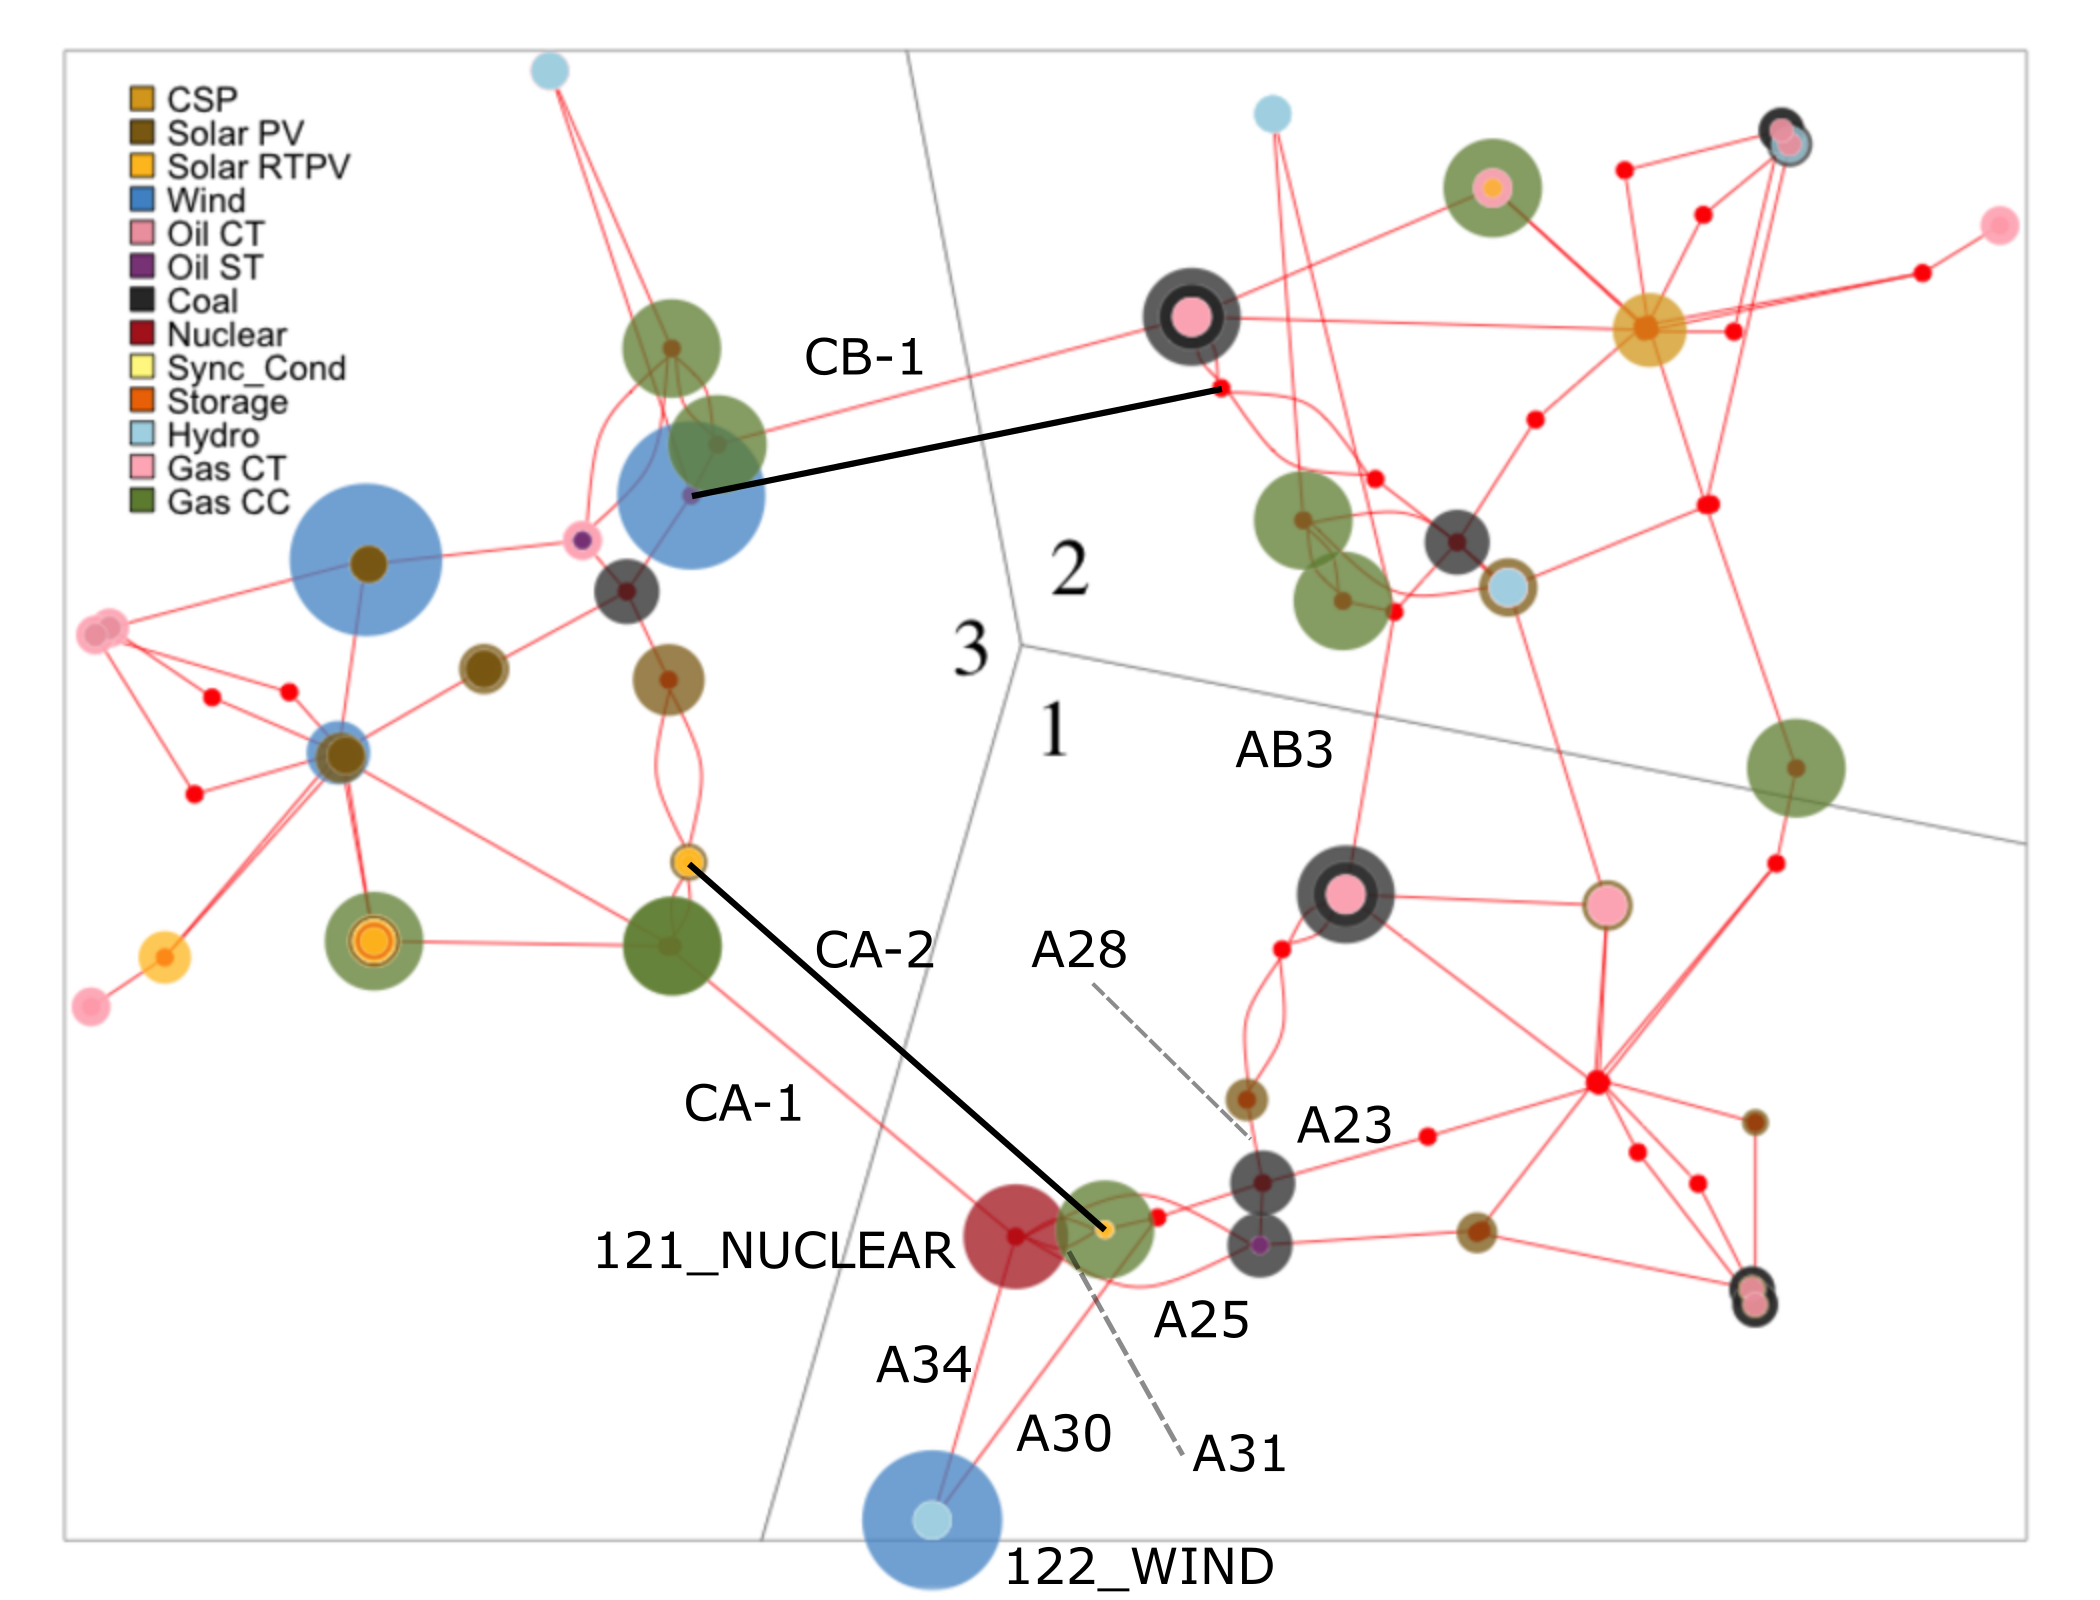
\includegraphics[width=0.8\linewidth]{Figs/RTS.png}
    \caption{Network layout of the RTS-GMLC from~\cite{RTS-GMLC}. New interconnections are represented in black.}
    \label{fig:RTS}
\end{figure}

For this work, two interconnections have been added to limit curtailment of the (very) large wind plants in zone 3 as shown in Figure~\ref{fig:RTS}. Other minor modifications have been done and are listed on \url{https://github.com/FredericSabot/PDSA-RTS-GMLC/tree/master/RTS-Data}. Hourly dispatches for typical days in January and July are shown in Figure~\ref{fig:dispatch}. The market model used is a locational marginal pricing (LMP) market model developed in~\cite{Prescient}. Figure~\ref{fig:dispatch} shows that high wind penetration (above 60\%) are sometimes reached especially for winter months during which load is relatively low. The RTS-GMLC data only includes a one-year time series realisation of renewable capacity factors and hydro inflows. Also, for the sake of simplicity, all assets (generation and transmission) are assumed to be always available. Therefore, only one MC year is considered.

\begin{figure}
\centering
\begin{tikzpicture}
\pgfplotsset{
/pgfplots/area cycle list/.style={/pgfplots/cycle list={%
{RedViolet,fill=red!75!black,mark=none},%
{black,fill=black,mark=none},%
{SeaGreen!40!white,fill=SeaGreen!40!white,mark=none},%
{LimeGreen!80!black,fill=LimeGreen!80!black,mark=none},%
% {pink,fill=pink,mark=none},%
{Cerulean,fill=Cerulean,mark=none},%
{Dandelion,fill=Dandelion,mark=none},%
}
},
}
\begin{groupplot}[
    group style={%
        columns=2,
        group name=plots,
        xlabels at=edge bottom,
        y descriptions at=edge left,
        horizontal sep =15pt,
    },
    xlabel = {Time [h]},
    ylabel = {Power [MW]},
    stack plots=y,%
    area style,
    xmin=0, xmax=24,
    xtick={0,8,16,24},
    ymin = 0, ymax=7500,
    tickpos=left,
    % ytick align=outside,
    % xtick align=outside,
    width=0.4\linewidth,
    height=0.4\linewidth,
]
\nextgroupplot
\addplot table [x=hour,y=nuclear] {Figs/dispatch_january.txt}
\closedcycle;
\addplot table [x=hour,y=coal] {Figs/dispatch_january.txt}
\closedcycle;
\addplot table [x=hour,y=hydro] {Figs/dispatch_january.txt}
\closedcycle;
\addplot table [x=hour,y=gas] {Figs/dispatch_january.txt}
\closedcycle;
% \addplot table [x=hour,y=oil] {Figs/dispatch_january.txt}
% \closedcycle;
\addplot table [x=hour,y=wind] {Figs/dispatch_january.txt}
\closedcycle;
\addplot table [x=hour,y=solar] {Figs/dispatch_january.txt}
\closedcycle;

\nextgroupplot[legend to name={DispatchLegend2},legend style={legend columns=6}]
\addplot table [x=hour,y=nuclear] {Figs/dispatch_july.txt}
\closedcycle;
\addplot table [x=hour,y=coal] {Figs/dispatch_july.txt}
\closedcycle;
\addplot table [x=hour,y=hydro] {Figs/dispatch_july.txt}
\closedcycle;
\addplot table [x=hour,y=gas] {Figs/dispatch_july.txt}
\closedcycle;
% \addplot table [x=hour,y=oil] {Figs/dispatch_july.txt}
% \closedcycle;
\addplot table [x=hour,y=wind] {Figs/dispatch_july.txt}
\closedcycle;
\addplot table [x=hour,y=solar] {Figs/dispatch_july.txt}
\closedcycle;

\legend{Nuclear, Coal, Hydro, Gas, Wind, Solar}

\end{groupplot}

\node[below] at (current bounding box.south)
      {\pgfplotslegendfromname{DispatchLegend2}};

\end{tikzpicture}
\caption{Market dispatch for a typical day in January (left) and July (right)}
\label{fig:dispatch}
\end{figure}

As there was no dynamic data in the original RTS-GMLC, they have been added in this thesis. Synchronous generators are represented with standard eighth order model and equipped with an IEEET1 exciter and a BPA GG (also known as WSCC type G) governor model as in~\cite{IEEE39Dynamic}. A different model is however used for hydro units as they have a fundamentally different behaviour than other types of units. The model used is an GOVHYDRO1 model. The machine, exciter and governor parameters are taken from annex D of~\cite{vittalBook}. This annex contains typical data for different types of machines (hydro, nuclear, coal, gas) and a wide range of rated powers (5~MW to 1.3~GW). So, for each generator of the test systems, parameters were taken from a machine in~\cite{vittalBook} that has the same type and that has the closest rated power. For hydro units, those parameters are completed with the ones in~\cite{hydroGov}. For inverter-based generation, the models from~\cite{ChaspierreThesis} are used. The protection system models (and associated uncertainty) are the same as in section~\ref{sec:protection_test_case} except load blinders have been added to distance protections. The blinders are set to avoid tripping for apparent impedances that correspond to a load of 150\% of the rated line current at 0.85~pu voltage and with a power factor angle of less than 30° following NERC recommendations~\cite{NERC_load_blinders}.

The contingencies considered in this example are three-phase faults occurring at one of the two extremities of lines. These faults are normally cleared by opening the faulted line in 100ms (N-1 contingency). However, it is also considered that there is a 0.1 probability that the primary protection fails and that the fault is thus cleared in 200ms (N-1 contingency with delayed clearing). Also, I consider a 0.01 probability that one breaker fails to open when clearing the fault. Breaker failure protection~\cite{HorowitzBook} is assumed to be installed in all substations and that they are able to clear the fault by opening a single adjacent line in 200ms (leading to an N-2 contingency). It has been checked that the system is always secure for N-1 contingencies with normal clearing time, these have thus not been considered in the PDSA. The contingencies listed above are line faults which are not cleared by the primary protection system due to protection failure or ``missed trips''. Another important class of protection failures are ``unwanted trips'', \ie trips that are not necessary to clear the fault and that thus unnecessarily disconnect elements. However, those are significantly more difficult to model as discussed in chapter~\ref{ch:protections} and are thus left for future work.

Only faults at the highest voltage level are considered which leads to a contingency list of 114 N-1 contingencies with delayed clearing and 594 N-2 contingencies. The frequency of line faults is taken as 2.5 faults per 100~km of line per year~\cite{FaultStatisticsFrance}\footnote{Due to lack of data, line fault probability is assumed independent of weather conditions. Fault and protection failure statistics significantly vary from country to country due to different weather and reliability and reporting practices (\eg \cite{GridPSA} reports a 0.27 fault per year and per 100~km of 400~kV overhead lines for the Finnish grid, while \cite{FaultStatisticsFrance} reports 2.5 in France). Data collection plans (as initiated by ENTSO-E~\cite{ENTSOE-PSA}) and failure mode and effect analysis (as demonstrated in~\cite{GridPSA}) should thus be performed to be able to fully trust the results of a PDSA.}.

The simulation of a given scenario provides with an estimate of the consequences of a contingency in terms of MW of load shed. This value can be translated into societal costs using the simple method described in section~\ref{sec:blackout_cost}. For the RTS and at average load (4350~MW), the cost of a complete blackout is thus estimated at 500M€. This is the value used for \(M_C\). Dynamic simulations are performed using \Dynawo{}~\cite{Dynawo} on 10 32-cores AMD EPYC Rome 7542 CPU's at 2.9 GHz.

Due to lack of time, loads where represented using a constant impedance load model in parallel with a simple motor model accounting for 30\% of the load. For grids with high shares of distributed energy sources, loads should instead be modelled using dynamic equivalents as discussed in chapter~\ref{ch:distrib}. The method proposed in chapter~\ref{ch:distrib} requires to simulate each scenario twice: once with 5-equivalents and once with 95-equivalents which double computation time. To limit this computation time, only the 95-equivalent could be used as it usually lead to more conservative results (especially for secure scenarios).

As for the other test cases in this thesis, the grid used in this example only has models for short-term stability as it is the focus of this thesis. However, while purely-fast cascades are becoming more common, there are still many cascades that start as slow cascades and latter transition to fast cascades if they cannot be stopped in the slow phase. To model these cascades that develop on a large range of timescales, it would be convenient to use simulators that can simulate such large ranges of timescales thanks to a variable integration time step such as Eurostag~\cite{STAG} or \Dynawo{}~\cite{Dynawo}. Alternatively, the slow and fast phases could be simulated separately as proposed in~\cite{TwoLevelPSA}. The advantage of this second approach is that more MC samples can be simulated during the slow phase (that is less computationally expensive to simulate). However, it requires predicting when a given cascade transition from the slow to the fast phase.



\section{Application of the proposed PDSA methodology}
\label{sec:PDSA_results}

This section describes the application of the proposed PDSA methodology to the RTS-GMLC with a focus on aspects related to sampling and computation time. The ``physical'' results will be described in section~\ref{sec:PDSA_interpretation} along with the discussion on how to use these results to enhance the security of the system.

% This section is organised similarly to the methodology section with section~\ref{sec:PDSA_results_sampling} discussing the sampling process and computational burden of the PDSA, section~\ref{sec:PDSA_results_screening} discussing the performance of the screening process and its impact on accuracy and computation time, section~\ref{sec:PDSA_results_protections} analysing the impact of protection-related uncertainties on fast cascading outages,


\subsection{Sampling of operating conditions}
\label{sec:PDSA_results_sampling}

A first PDSA has been performed without screening of scenarios to be used as a reference. An \(\epsilon\) of 1\% has been used in this example for the stopping criterion~(\ref{eq:stop}). The main results of this analysis are given in Table~\ref{tab:summary-N1N2}. It shows that N-1 contingencies with delayed clearing and N-2 contingencies have a similar contribution to the total risk. Also, while there are more N-2 contingencies than N-1 contingencies (594 vs 114), N-2 contingencies require fewer simulations, and therefore less computation time than N-1 contingencies. In total, 152,138 scenarios are considered, leading to 157,346 simulations (to account for protection-related uncertainties). 4329 scenarios are found to be unsecure, and 7 lead to convergence issues in the time-domain simulation. This relatively small number of unsecure scenarios indicates that screening of scenarios could significantly reduce computation time.

\begin{table}
\centering
\caption{Contribution to total risk and computation time of delayed clearing N-1 contingencies and N-2 contingencies (without screening)}
\label{tab:summary-N1N2}
\begin{tabular}{@{}lll@{}}
\toprule
                                 & N-1 with delayed clearing  & N-2 \\ \midrule
Risk (M€/y) & 8.6 & 12.4 \\
Number of simulations            & 97,503 & 59,648 \\
Computation time (core-h)        & 1046  & 656 \\
Average computation time per simulation (s) & 38.6 & 39.6 \\ \bottomrule
\end{tabular}
\end{table}


This is because N-1 contingencies (with delayed clearing) are contingencies that are more frequent than N-2 contingencies but infrequently lead to significant consequences. It is thus necessary to sample many operating conditions to obtain a statistically accurate risk and guarantee a sufficient coverage of the likely operating conditions.

Figure~\ref{fig:indic_N1} (resp. Figure~\ref{fig:indic_N2}) shows the number of simulations performed for all N-1 (resp. N-2) contingencies and the associated standard error (decomposed in terms of variance and coverage). It shows that for most contingencies the coverage part of the SE is dominant compared to the variance part. For these contingencies, the SE bound reduces to

\begin{equation}
  SE_i \lesssim \frac{f_i}{N_i} \sqrt{3 \beta_i^2}
\end{equation}

\noindent and the number of simulations needed to satisfy the stopping criterion (\ref{eq:stop}) is thus directly proportional to the frequency of the contingency. For contingencies with non-negligible variance, the number of simulations needed is higher which explains the spikes of \(N_i\) in Figure~\ref{fig:indic_N1} and Figure~\ref{fig:indic_N2}.


\begin{figure}
\centering
\begin{tikzpicture}
\pgfplotsset{width=0.8\linewidth}
\begin{groupplot}[
    group style={
        group name=my plots,
        group size=1 by 2,
        xlabels at=edge bottom,
        xticklabels at=edge bottom,
        vertical sep=20pt,
    },
    width=0.8\linewidth,
    height=5cm,
    xlabel=Contingency ID,
    xmin=1, xmax=114,
    ymin=0,
    yticklabel style={/pgf/number format/fixed},
    tickpos=left,
    ytick align=outside,
    xtick align=outside,
]
\nextgroupplot[ylabel=\(N_i\), height=4cm]
\addplot+ [mark=none] table [x=id,y=N_static] {Figs/N_N1.txt};

\nextgroupplot[
    ylabel style={align=center}, ylabel=Statistical accuracy\\{[M€/y]},
    legend style={legend columns=2}, ymax=0.34]

\addplot+ [ybar interval, fill, mark=none] table [x=id,y expr=\thisrow{indic_1}*1.609344] {Figs/N_N1.txt};  % TODO: remove mi to km conversion if computations are rerun
\addplot+ [mark=none] table [x=id,y expr=\thisrow{indic_2}*1.609344] {Figs/N_N1.txt};
\addlegendentry{Variance}
\addlegendentry{Coverage}
\end{groupplot}
\end{tikzpicture}
\caption{Number of sampled operating conditions and statistical accuracy for all delayed-clearing N-1 contingencies sorted in decreasing order of likelihood}
\label{fig:indic_N1}
% \end{figure}
\vspace{0.7cm}
% \begin{figure}
\centering
\begin{tikzpicture}
\pgfplotsset{width=0.8\linewidth}
\begin{groupplot}[
    group style={
        group name=my plots,
        group size=1 by 2,
        xlabels at=edge bottom,
        xticklabels at=edge bottom,
        vertical sep=20pt,
    },
    width=0.8\linewidth,
    height=5cm,
    xlabel=Contingency ID,
    xmin=1, xmax=594,
    ymin=0,
    yticklabel style={/pgf/number format/fixed},
    tickpos=left,
    ytick align=outside,
    xtick align=outside,
]
\nextgroupplot[ylabel=\(N_i\), height=4cm]
\addplot+ [mark=none] table [x=id,y=N_static] {Figs/N_N2.txt};

\nextgroupplot[
  ylabel style={align=center}, ylabel=Statistical accuracy\\{[M€/y]},
  legend style={legend columns=2}, ymax=0.34]

  \addplot+ [ybar interval, fill, mark=none] table [x=id,y expr=\thisrow{indic_1}*1.609344] {Figs/N_N2.txt};
  \addplot+ [mark=none] table [x=id,y expr=\thisrow{indic_2}*1.609344] {Figs/N_N2.txt};
\addlegendentry{Variance}
\addlegendentry{Coverage}
\end{groupplot}
\end{tikzpicture}
\caption{Number of sampled operating conditions and statistical accuracy for all N-2 contingencies sorted in decreasing order of likelihood}
\label{fig:indic_N2}
\end{figure}


It is interesting to see that when aiming to minimise the SE of the risk contribution of \emph{individual} contingencies, the best strategy is basically to use a crude MC approach (\ie sampling contingencies proportionally to their frequency of occurrence) (except for a few contingencies with high variance). In a crude MC approach, the total risk can be estimated as

\begin{equation}
  R = \left(\sum_i f_i\right) \left(\frac{1}{N} \sum_s c_s\right)
\end{equation}

\noindent where \(c_s\) are the consequences of the \(s\)th sample (random contingency and initial state). Using the same development as to derive equation~\ref{eq:SE_bound}, the following bound can be obtained for the SE of the total risk.

\begin{equation}
  \label{eq:SE_total}
  SE \leq \left(\sum_i f_i\right) \sqrt{\frac{\tilde{\sigma}^2}{N} + \frac{3 \beta^2}{N^2}}
\end{equation}

\noindent where \(\tilde{\sigma}\), \(\beta\), and \(N\) have the same definitions as \(\tilde{\sigma_i}\), \(\beta_i\), and \(N_i\) but for the total risk instead of individual contingencies. Figure~\ref{fig:SE_total} shows how this SE evolves with the number of samples. After 150,000 samples (roughly the number of simulations performed in this study, cf. Table~\ref{tab:summary-N1N2}), the coverage term of SE is 4.3 smaller than the variance term while it was strongly dominant for the SE of individual contingencies. This is because the coverage term accounts for the likelihood of having missed unsecure regions during sampling, and while this likelihood is relatively high for individual contingencies, it is unlikely to miss unsecure regions for all of them. Figure~\ref{fig:SE_total} shows the coverage term becomes smaller than the variance term after roughly 8000 samples. Thus, if one is only interested in the total risk and not in the risk of individual contingencies (for some reason), then variance-reduction techniques become viable after this point.

\begin{figure}
\centering
\begin{tikzpicture}
\pgfplotsset{width=0.6\linewidth}
\begin{axis}[
    xlabel={Number of samples},
    xmin=1000, xmax=150000,
    ymin=0, ymax=8,
    xmode=log,
    grid,
    log ticks with fixed point,
    ylabel= {SE [M€/y]},
    legend cell align=left,
    legend style={at={(1,1)},anchor=north east},
    ]

    \addplot+ [mark=none, dashed] table [x=x,y expr=\thisrow{sigma}*1.609344] {Figs/total_risk_SE.txt};
    \addplot+ [mark=none, dashdotted] table [x=x,y expr=\thisrow{coverage}*1.609344] {Figs/total_risk_SE.txt};
    \addplot+ [mark=none] table [x=x,y expr=\thisrow{SE}*1.609344] {Figs/total_risk_SE.txt};
    \addplot+ [mark=none, gray, dashed, domain=500:150000, samples=2] {0.05 * 13.226341374847571 * 1.609344};

    \addlegendentry{Variance}
    \addlegendentry{Coverage}
    \addlegendentry{Total SE}
    \addlegendentry{5\% of total risk}

\end{axis}
\end{tikzpicture}
\caption{Evolution of the SE of the total risk with the number of samples}
\label{fig:SE_total}
\end{figure}

\begin{figure}
  \centering
  \begin{tikzpicture}
  \pgfplotsset{width=0.8\linewidth}
  \begin{axis}[
      height=5cm,
      xlabel=Contingency ID,
      xmin=0.5, xmax=20.5,
      ymin=0,
      yticklabel style={/pgf/number format/fixed},
      ylabel=Risk {[M€/y]},
      xtick={1,2,...,20},
  ]

  \addplot+ [ybar, ybar legend, fill, mark=none, bar width=5pt] table [x=id,y expr=\thisrow{cost}*1.609344] {Figs/critical_SE.txt};
  \addplot+ [mark=none, domain=0:21] {0.01 * 13.226341374847571 * 1.609344};

  \addlegendentry{Risk}
  \addlegendentry{\(SE_i\)}

  \end{axis}
  \end{tikzpicture}
  \caption{Risk of the 20 most critical contingencies and associated SE}
  \label{fig:SE_individual}
\end{figure}

It can be noted that, for a given number of samples, the statistical accuracy of the total risk estimate is better than the one of the individual contingencies. Indeed, Figure~\ref{fig:SE_total} shows that with 150,000 samples, the SE of the total risk is smaller than 5\%. On the other hand, Figure~\ref{fig:SE_individual} shows a SE higher than 50\% for all contingencies except the 10 most critical ones. This figure shows that, with the chosen value of \(\epsilon\) (1\%), the 10 most critical contingencies are most likely correctly identified. The individual risk associated with the remaining contingencies is close to or smaller than \(SE_i\), so there is a chance that contingencies with a higher risk have been missed in the analysis. Instead of \(SE_i < \epsilon R\), it would be possible to define the stopping criteria such that \(SE_i\) must be smaller than, \eg, the risk of the tenth most critical contingency. This would remove the need to manually set a value for \(\epsilon\), however, this could cause the computation to never or slowly converge in case the tenth most critical contingency has a very low risk contribution (\ie if the risk is dominated by the first nine contingencies).


\subsection{Sampling of protection-related uncertainties}
\label{sec:PDSA_results_protections}

The results discussed above have been obtained by running 5 MC simulations for each scenario for which protection-related uncertainties are expected to have an impact. This was the case for a fifth (834 out of 4329) of unsecure scenarios. Of these, half (408 out of 834) led to different consequences depending on the sampled protection system parameters. In the remaining half, the cascading path was affected by protection-related uncertainties, but the final consequences were not. As discussed in section~\ref{sec:protection_results}, there are two main reasons for this. The first is that changing the order of protection operations does not always impact the general evolution of the cascade. The second is that the operation of an additional protection system does not necessarily impact the consequences, for example, if it occurs in an island of the system that will nevertheless collapse.

Performing 5 MC simulations for each scenario impacted by protection-related uncertainties can be viewed as a way to perform importance sampling. However, as shown above, a crude MC approach is more efficient for most contingencies. Theoretically, it would thus be more efficient to draw one sample of protection-related parameters for each sample of operating conditions. But in practice, the proposed approach gives more intuitive results because it allows one to separate the impact of operating conditions and of protection parameters.

Also, it can be argued that using an indicator to predict which scenarios are sensitive to protection-related uncertainties increases coverage as one sample directly accounts for all possible values of protection parameters, reducing the dimension of the uncertainty space and the likelihood of missing critical regions. In any case, the impact on computation time is relatively limited as the scenarios that are secure and not affected by protection-related uncertainties take most of the computation time.


% Comparing MC algorithms is often performed using a Figure of Merit (FoM)
%
% \begin{equation}
% FoM_i = \frac{1}{\tilde{\sigma_i}^2 N^T_i}
% \end{equation}
%
% where \(R_i\) is the risk associated to contingency \(i\), and \(N^T_i\) is the total number of simulations performed for contingency \(i\). Fig.~\ref{fig:FoM} shows that the PDSA performed without the indicator has a higher FoM and is thus more efficient for most of the contingencies. Despite the above, we still recommend the use of the indicator as (i) it helps in the interpretation of the simulation results by decoupling the impact of static and protection-related uncertainties, and (ii) it acts as a form of robustness analysis (for protection-related uncertainties only), at the cost of a small increase in computation time.
%
% \begin{figure}  % FoM figure should be updated (sigma should be lower with indicator). Anyway, this neglects coverage, so not super useful
% \centering
% \begin{tikzpicture}
% \pgfplotsset{width=0.8\linewidth}
% \begin{groupplot}[
%     group style={
%         group name=my plots,
%         group size=1 by 3,
%         xlabels at=edge bottom,
%         xticklabels at=edge bottom,
%         vertical sep=20pt
%     },
%     height=4cm,
%     xlabel=Contingency ID,
%     xmin=1, xmax=10,
%     ymin=0,
%     tickpos=left,
%     ytick align=outside,
%     xtick align=outside,
% ]
% \nextgroupplot[ylabel=\(S_i\) {[\%]}, ymax=50]
% \addplot+ [mark=none] table [x=id,y=share] {Figs/FoM.txt};
% \nextgroupplot[
%     ylabel=\(\sigma_i\),
%     legend cell align=left,
%     legend style={at={(1,1)},anchor=north east}]
% \addplot+ [mark=none] table [x=id,y=std_dev] {Figs/FoM.txt};
% \addplot+ [mark=none] table [x=id,y=std_dev_no_indic] {Figs/FoM.txt};
% \nextgroupplot[
%     ylabel=\(FoM_i\),
%     legend to name={CommonLegend},legend style={legend columns=2}]
% \addplot+ [mark=none] table [x=id,y=FoM] {Figs/FoM.txt};
% \addplot+ [mark=none] table [x=id,y=FoM_no_indic] {Figs/FoM.txt};
% \addlegendentry{With indicator}
% \addlegendentry{Without indicator}
% \end{groupplot}
% \node[below] at (current bounding box.south)
%       {\pgfplotslegendfromname{CommonLegend}};
% \end{tikzpicture}
% \caption{Share of operating conditions \(S_i\) for which protection-related uncertainties have an impact, standard deviation \(\sigma_i\), and figure of merit \(FoM_i\) of the 10 N-2 contingencies with the largest \(S_i\)}
% \label{fig:FoM}
% \end{figure}


\subsection{Missing trips during cascades}
\label{sec:PDSA_results_missing_trips}

Some works (\eg~\cite{Faghihi, DCATphase1}) consider that there might be ``missing trips'' during the evolution of the cascade. Indeed, each time a protection system operates during a cascade, there is also some probability that it fails to operate. This can be considered by splitting the simulation in two branches when one protection operates: one where the protection actually operates and one where it fails to; each associated with some probability.

Due to time constraints, this has not been considered in this thesis. However, an estimation of the risk associated with those missing trips can be done based on the results of the present analysis. Indeed, for each simulation performed, the associated sequence of tripping events is saved to allow for further analysis. The frequency of protection system operations (not accounting for fault clearing) can thus be estimated at 0.35 per year. This can be compared to the 17.9 contingencies per year of the RTS (11.7 for delayed-clearing N-1 contingencies and 6.2 for N-2 contingencies). This figure does not account for under-frequency load shedding (UFLS) relay trips because the failure of a single UFLS relay is unlikely to affect the evolution of a cascade. Generator protections are also not included in this figure as missing trips of generators are made very unlikely due to the high consequences for the generator if it is not disconnected when needed.

Based on this figure, assuming a probability of protection failure to operate of 0.01, and assuming that any protection system failure to operate during a cascade leads to a full blackout leads to a risk of 2.83~M€/y. This risk is thus negligible compared to the 28.8~M€/y risk computed without considering the possible failure of protection to operate during cascades. Moreover, this 2.83~M€/y figure is very conservative as it assumes all protection failures to operate lead to a full blackout. Actually, since most protection systems aim to protect individual elements and not the grid itself, a failure to operate during a cascade will not necessarily have a negative impact on the cascade propagation. The failure of system integrity protection schemes could be considered. However, they are often designed to have a very high level of reliability, so it would make more sense in a possibilistic approach rather than a probabilistic one.

This section has discussed the risk associated with missing trips, but, as discussed previously, unwanted trips (both directly following fault clearing and during the cascade propagation) should be studied in further work.


\subsection{Screening}
\label{sec:PDSA_results_screening}

We now study how the addition of a screening process impacts the accuracy and computational burden of the PDSA. The main results are given in Table~\ref{tab:screening}. First, it is important to notice that even though the contingencies considered in this analysis are relatively severe (compared to the N-1 contingencies with normal clearing time the system has been designed to withstand), only 3\% of the sampled scenarios (4329 out of around 152,138) lead to consequences (around 2\% for delayed-clearing N-1 scenarios, and 4\% for N-2 scenarios). Therefore, without screening, 95\% of the computation time is wasted on secure scenarios (not 97\%, as an unsecure scenario takes on average more time to simulate than a secure one).

With perfect screening, the computational burden of the PDSA can thus be reduced by a factor 20. The screening process used in this work does not reach this performance however. It has a low false negative (FN) rate, \ie very few unsecure scenarios are missed, so it has a low impact on the PDSA accuracy (only 4\% of the total risk is missed). However, it has a high false positive (FP) rate, \ie many secure scenarios are flagged as unsecure and therefore unnecessarily simulated. Screening thus only speeds up the PDSA by a factor 1.94, way less than the theoretical limit of 20.

\begin{table}
  \centering
  \caption{Performance of the screening process and impact on the PDSA accuracy and computation time}
  \label{tab:screening}
  \begin{tabular}{@{}lllllll@{}}
    \toprule
    \multirow{2}{*}{Contingencies} &
      \multicolumn{2}{l}{Unsecure cases} &
      \multicolumn{2}{l}{Secure cases} &
      \multirow{2}{*}{\begin{tabular}[c]{@{}l@{}}Missed\\ risk (\%)\end{tabular}} &
      \multirow{2}{*}{Speed-up} \\ \cmidrule(lr){2-3} \cmidrule(lr){4-5}
        & FN & TP   & FP     & TN     &     &      \\ \midrule
    N-1 with delayed clearing & 4  & 1553 & 40,100 & 52,400 & 0.3 & 2.01 \\
    N-2 & 81 & 1847 & 22,300 & 25,200 & 6.4 & 1.81 \\
    All & 85 & 3400 & 62,400 & 77,800 & 4.0 & 1.94 \\ \bottomrule
  \end{tabular}
\end{table}

This is mainly because the EEA underestimate CCT in this case due to the large penetration of inverter-based generators. Indeed, due to their low capacity factors, inverter-based generators often have room to provide fast voltage support which helps with the angular stability of synchronous generators. Table~\ref{tab:CCT_margin} shows that when using a CCT margin of -20ms in the screening process, \ie assuming that faults cleared in 200ms are secure if the EEA predicts a CCT larger than 180ms, a speed-up of 3.5 can be obtained but at the cost of missing 16.6\% of the total risk. Better stability indicators should be developed if higher speed-ups and/or lower impact on accuracy are desired.

\begin{table}
  \centering
  \caption{Impact of the CCT margin on screening performance}
  \label{tab:CCT_margin}
  \begin{tabular}{@{}lll@{}}
  \toprule
  CCT margin (ms) & Missed risk (\%) & Speed-up \\ \midrule
  50  & 4.0  & 1.94 \\
  0   & 9.3  & 2.75 \\
  -20 & 16.6 & 3.49 \\ \bottomrule
  \end{tabular}
\end{table}

It should be noted that the screening does not affect the risk estimate of all contingencies in the same way. In the case of the negative 20ms CCT margin, the risk estimates for the first 10 most critical contingencies are not affected by the screening process, except for the 2nd most critical contingency that is almost entirely missed and the 4th whose risk is underestimated by 25\%. With 0 margin, the risk of the 2nd most critical contingency is underestimated by 35\% which is more acceptable. With a positive 50ms margin, none of the first 10 most critical contingencies are underestimated by the screening process.

% 0.18 CCT threshold
% Rank 2, A25-1_end1-BREAKER_end1-A25-2, misses: 55/82, max shedding: 100.0
% Rank 4, A23_end2-BREAKER_end2-A28, misses: 6/22, max shedding: 100.0
% Rank 6, C22_end1_DELAYED, misses: 1/146, max shedding: 10.0
% Rank 11, A23_end1-BREAKER_end2-A28, misses: 7/7, max shedding: 100.0
% Rank 12, A27_end2-BREAKER_end1-A24, misses: 4/5, max shedding: 100.0
% Rank 14, CA-2_end2_DELAYED, misses: 1/9, max shedding: 67.84
% Rank 17, B21_end2_DELAYED, misses: 2/73, max shedding: 3.495
% Rank 18, A27_end1-BREAKER_end1-A24, misses: 2/5, max shedding: 100.0

% 0.2
% Rank 2, A25-1_end1-BREAKER_end1-A25-2, misses: 30/82, max shedding: 100.0
% Rank 4, A23_end2-BREAKER_end2-A28, misses: 1/22, max shedding: 100.0
% Rank 6, C22_end1_DELAYED, misses: 1/146, max shedding: 10.0
% Rank 11, A23_end1-BREAKER_end2-A28, misses: 7/7, max shedding: 100.0
% Rank 12, A27_end2-BREAKER_end1-A24, misses: 1/5, max shedding: 100.0
% Rank 18, A27_end1-BREAKER_end1-A24, misses: 1/5, max shedding: 100.0

% 0.25
% Rank 11, A23_end1-BREAKER_end2-A28, misses: 7/7, max shedding: 100.0
% Rank 22, A28_end2-BREAKER_end1-A23, misses: 4/6, max shedding: 100.0

\section{Interpreting the results and enhancing security}
\label{sec:PDSA_interpretation}

Once all necessary simulations have been performed, the results of the PDSA can be analysed. A first intuitive interpretation of the results is proposed in section~\ref{sec:PDSA_results_intuitive}. However, as the PDSA produces thousands of unsecure scenarios (and even more secure ones), it is not possible to review each scenario in details. To alleviate this issue, machine learning techniques can be used. Basic machine learning techniques are thus used in section~\ref{sec:PDSA_ML} to help with the interpretation of the results and to enhance the security of the system.

\subsection{Intuitive interpretation of the results}
\label{sec:PDSA_results_intuitive}

Table~\ref{tab:critical_contingencies} shows a summary of the PDSA results for the 10 most critical contingencies. It should be noted that these 10 contingencies (out of 708) contribute for 44\% of the total risk. This shows that significant reduction of the risk could potentially be obtained by targetting those specific contingencies. Moreover, most of these contingencies concern lines that are in the same region (in the South of Figure~\ref{fig:RTS-copy}) highlighting the potential to solve multiple issues in one go.

\afterpage{%
\clearpage% Flush earlier floats (otherwise order might not be correct)
% \thispagestyle{empty}% empty page style (actually fine with headers)
\begin{landscape}% Landscape page
\centering

\begin{figure}
\centering
\begin{minipage}{\linewidth}
\begin{minipage}[c]{0.58\linewidth}
  \strut\vspace*{-\baselineskip}\newline % Minipage vertical allignement black magic
  % \centering
  \captionof{table}{Results of the PDSA for the 10 most critical contingencies. Line locations are given in Figure~\ref{fig:RTS-copy}.}
  \vspace*{0.5\baselineskip}
  \begin{tabular}{@{}lllllll@{}}
    \toprule
    \multicolumn{2}{c}{Contingency} &
      \multirow{2}{*}{\begin{tabular}[c]{@{}l@{}}Risk\\ {[}M€/y{]}\end{tabular}} &
      \multirow{2}{*}{\begin{tabular}[c]{@{}l@{}}Frequency\\ {[}/y{]}\end{tabular}} &
      \multirow{2}{*}{\begin{tabular}[c]{@{}l@{}}Share of unsecure\\ operating points {[}\%{]}\end{tabular}} &
      \multicolumn{2}{c}{Load shed {[}\%{]}} \\ \cmidrule(r){1-2} \cmidrule(l){6-7}
    Fault  & Adj. line &        &         &      & Mean\(^a\) & Max  \\ \midrule
    A34    & /         & 2.22  & 0.12   & 20.3 & 28.0 & 100  \\
    A25-1  & A25-2     & 1.87  & 0.017  & 18.9 & 69.7 & 100  \\
    CA-1   & /         & 1.66  & 0.17   & 11.6 & 21.4 & 100  \\
    A23    & A28       & 0.72 & 0.0068  & 18.3 & 81.9 & 100  \\
    CB-1   & /         & 0.68 & 0.18    & 8.5  & 15.4 & 36.5 \\
    C22    & /         & 0.60 & 0.15    & 12.2 & 10.8 & 25   \\
    A34    & A25       & 0.56 & 0.012   & 38.0 & 30.3 & 100  \\
    AB3    & /         & 0.56 & 0.13    & 7.1  & 15.5 & 100  \\
    A25    & /         & 0.55 & 0.17    & 6.8  & 14.5 & 91.3 \\
    A34    & CA-1      & 0.51 & 0.012   & 32.7 & 33.4 & 94.5 \\
    Others & /         & 12.4 & 17.0    & /    & /    & 100  \\ \bottomrule
    \multicolumn{7}{l}{\(^a\) Mean load shedding accounts for unsecure operating points only} \\
    \end{tabular}
  \label{tab:critical_contingencies}
\end{minipage}
\hfill
\begin{minipage}[c]{0.42\linewidth}
  \strut\vspace*{-\baselineskip}\newline % Minipage vertical allignement black magic
  \centering
  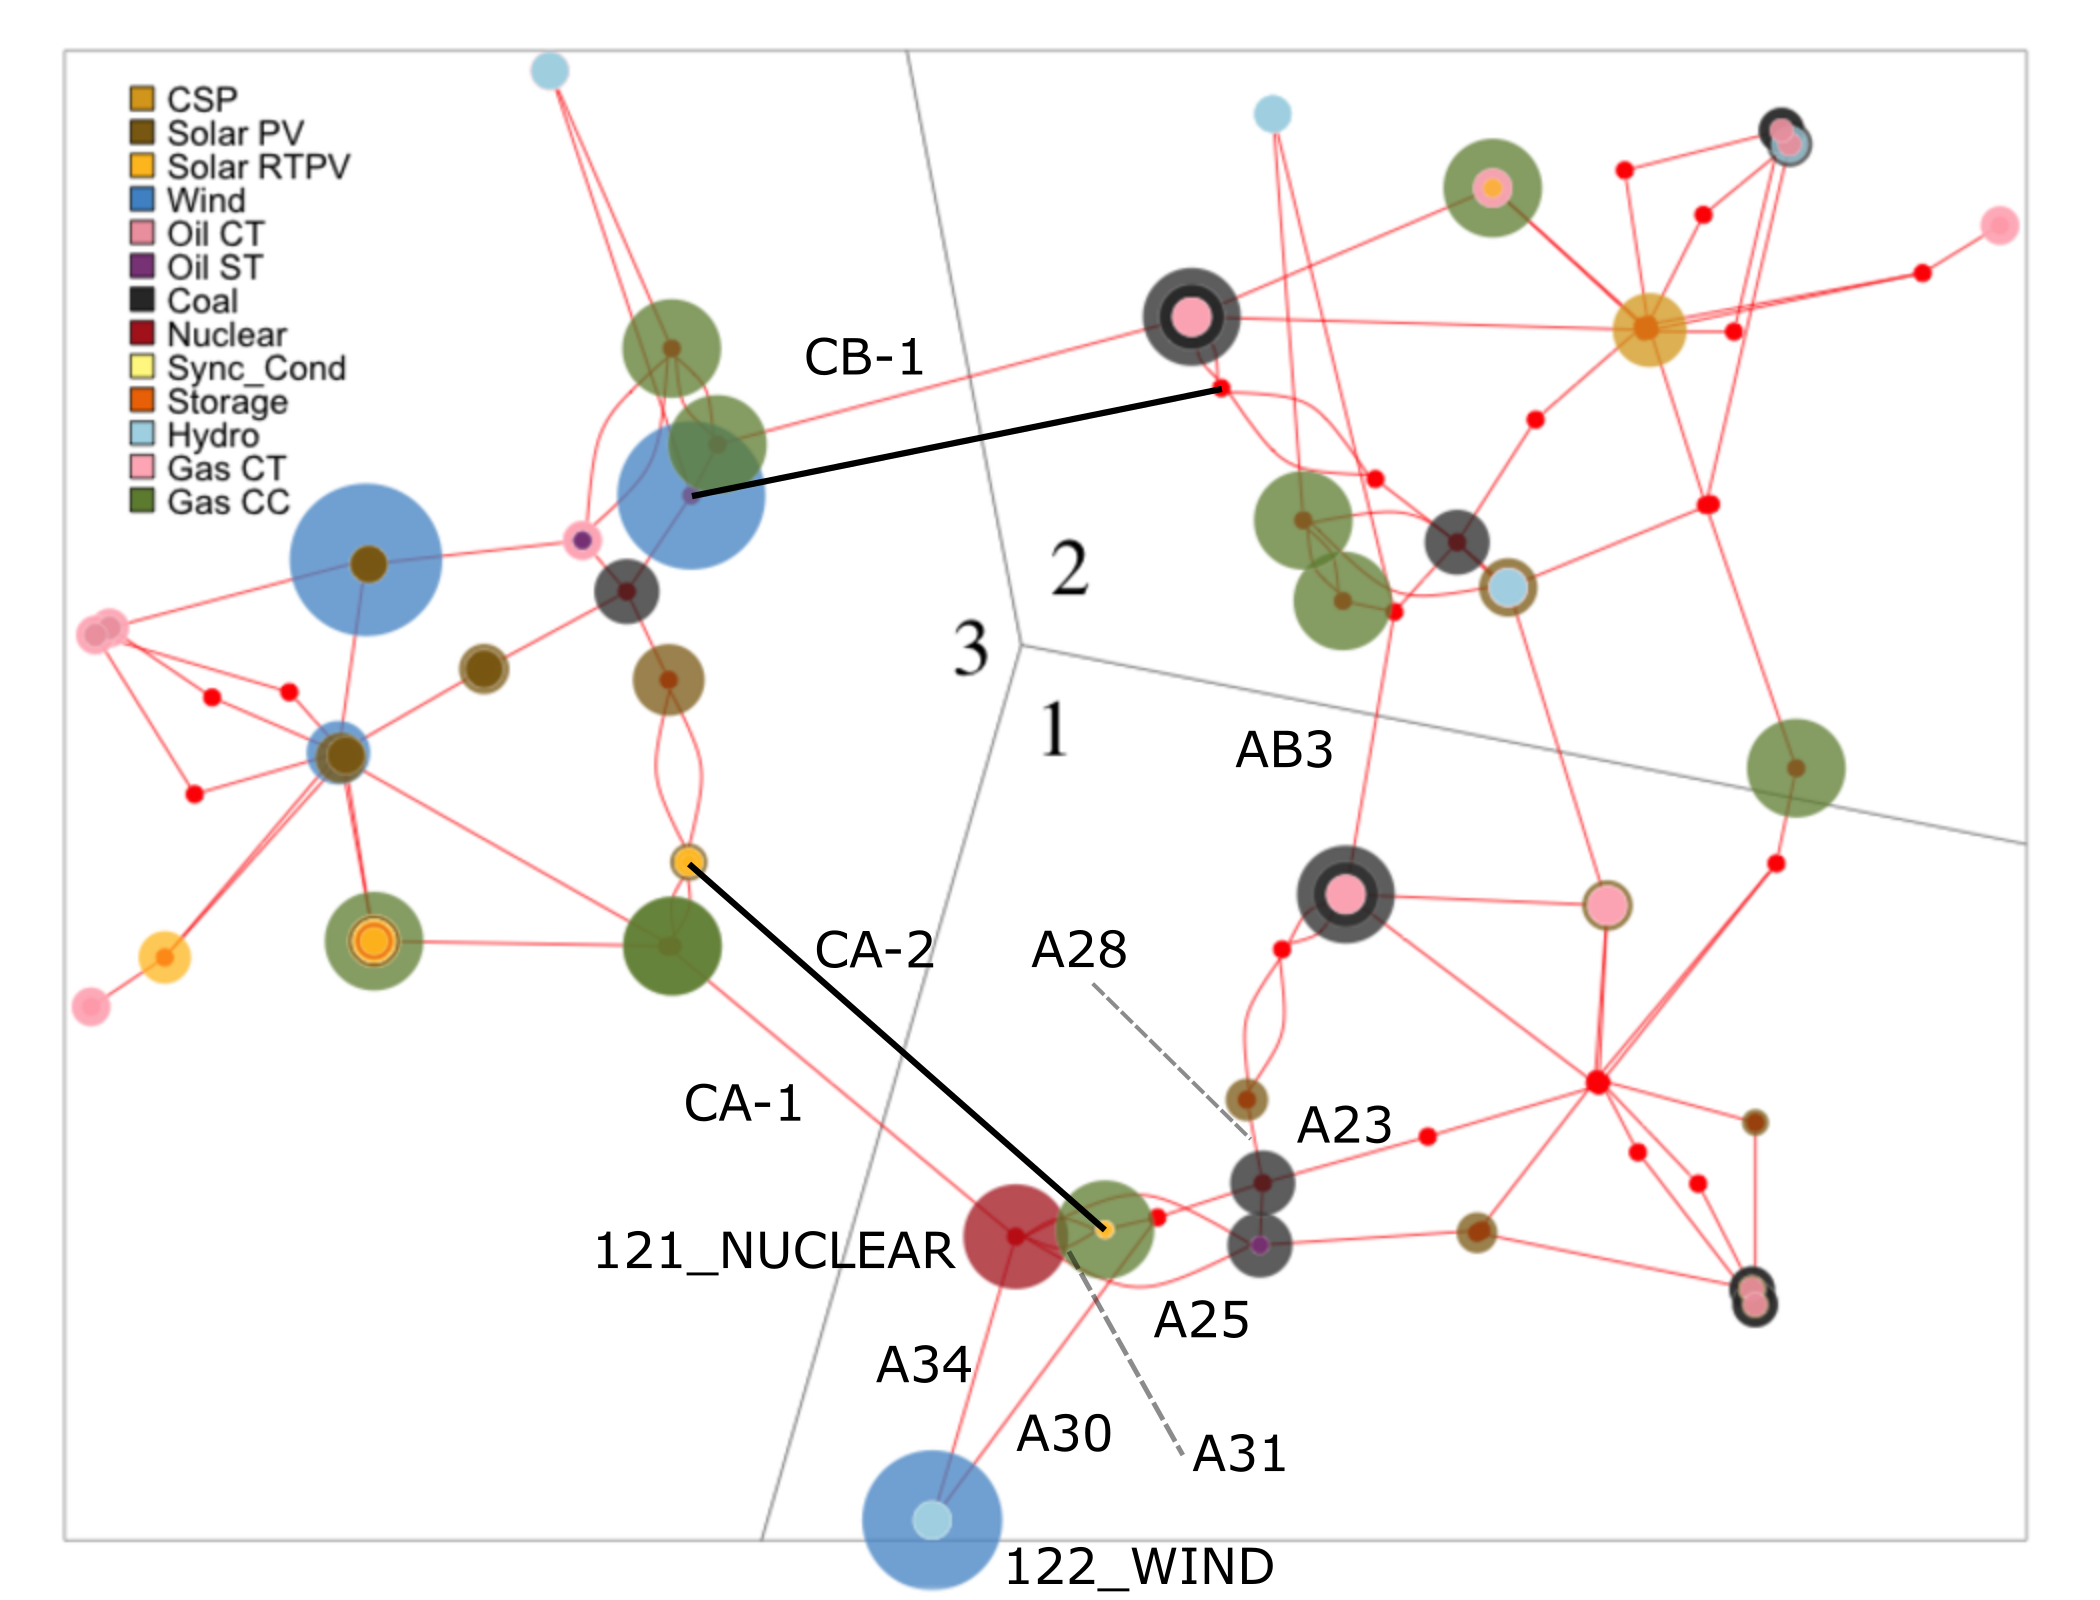
\includegraphics[width=0.8\linewidth]{Figs/RTS.png}
  \captionof{figure}{Network layout of the RTS-GMLC copied from Figure~\ref{fig:RTS} for convenience}
  \label{fig:RTS-copy}
\end{minipage}
\end{minipage}
\end{figure}


\begin{table}
\centering
\caption{Examples of samples for the most critical contingency (fault on line A34 with delayed clearing). Trips beyond the first three are not shown.}
\label{tab:samples_A34}
\begin{tabular}{@{}lllllll@{}}
  \toprule
  \begin{tabular}[c]{@{}l@{}}Hour\\ of year\end{tabular} & \begin{tabular}[c]{@{}l@{}}Load\\ shedding {[}\%{]}\end{tabular} & Trip 1 & Trip 2 & Trip 3 & \begin{tabular}[c]{@{}l@{}}Uncertain\\ protection impact\end{tabular} & \begin{tabular}[c]{@{}l@{}}Share of scenarios\\ with same initial 2 trips\end{tabular} \\ \midrule
  4633 & 0  & /                           & /                         & /                     & No            & 73.8 \\
  4103 & 51 & A30\_side2\_Distance\(^a\)  & 121\_NUCLEAR\_Angle\(^b\) & 122\_WIND\(^c\)       & Missing trips & 2.2  \\
  7634 & 40 & 121\_NUCLEAR\_Angle         & A30\_side2\_Distance      & 122\_WIND             & No            & 10.0 \\
  291  & 0  & 121\_NUCLEAR\_Angle         & /                         & /                     & No            & 5.3  \\
  8402 & 10 & 121\_NUCLEAR\_Angle         & UFLS\(^d\)                & /                     & No            & 3.9  \\
  8686 & 42 & A30\_side2\_Distance        & CA-1\_side1\_Distance     & 122\_WIND             & Missing trips & 0.6  \\
  1446 & 90 & CA-2\_side2\_Distance       & CA-1\_side2\_Distance     & A30\_side2\_Distance  & Missing trips & 0.8  \\ \bottomrule
  \multicolumn{6}{l}{\(^a\) Trip of line A30 by the distance protection on the second side of the line} \\
  \multicolumn{6}{l}{\(^b\) Trip of the nuclear power plant at bus 121 following loss of synchronism} \\
  \multicolumn{6}{l}{\(^c\) Trip of the wind farm at bus 122} \\
  \multicolumn{6}{l}{\(^d\) Under-frequency load shedding} \\
  \end{tabular}
\end{table}

% 73.8425925925926 ()
% 10.030864197530864 ('121_NUCLEAR_1_InternalAngle', 'A30_side2_Distance')
% 5.324074074074074 ('121_NUCLEAR_1_InternalAngle',)
% 3.8580246913580245 ('121_NUCLEAR_1_InternalAngle', 'UFLS')
% 2.2376543209876543 ('A30_side2_Distance', '121_NUCLEAR_1_InternalAngle')
% 0.7716049382716049 ('CA-2_side2_Distance', 'CA-1_side2_Distance')
% 0.6172839506172839 ('A30_side2_Distance', '122_WIND_1')

\end{landscape}
\clearpage% Flush page
}


However, Table~\ref{tab:critical_contingencies} does not explain why those contingencies are unsecure nor how to make them more secure. Table~\ref{tab:samples_A34} does a first step by showing a few samples (7 out of 1274) of the most critical contingency (fault on line A34 with delayed fault clearing). The table shows that the contingency can lead to different trip sequences depending on the operating conditions leading to different consequences. Actually, upon further analysis, all sequences are initiated due to the loss of synchronism of the nuclear power plant located in bus 121 (121\_NUCLEAR in Figure~\ref{fig:RTS-copy}).

Indeed, Figure~\ref{fig:A34_voltage} shows the voltage evolution for two of these cases (hours 7634 and 8402). In both cases, voltage at some buses stay depressed after fault clearing due to the loss of synchronism of the nuclear generator. Also, following the fault, line A34 is disconnected and the wind farm at bus 121 (121\_WIND) only remain connected to the rest of the system through line A30. And due to the depressed voltages, the wind farm is not able to push its power through this single line (that connects bus 121 to bus 117). In some cases (\eg Figure~\ref{fig:A34_voltage_7634}), this leads to trip of line A30 by distance protection. In other cases (\eg Figure~\ref{fig:A34_voltage_8402}), the distance protection of line A30 is armed, but the nuclear generator is disconnected, allowing for voltages to recover before the distance protection sends a trip signal.

These different possible sequences lead to different consequences. Indeed, in the former, both a nuclear power plant (of 400~MW) and a large wind farm (750~MW installed capacity, compared to the total load that varies between 3 and 7.5~GW) are disconnected leading to 30 to 50\% of load shedding (depending on operating conditions) by UFLS relays. In the latter, only the nuclear power plant is disconnected, so at most 15\% of the load has to be shed.

The two last cases in Table~\ref{tab:samples_A34} are also initiated by the loss of synchronism of the nuclear power plant at bus 121, however, they also lead to the disconnection of lines CA-1 and CA-2 that connect regions 1 and 3 together (by distance protection due to high flows from region 1 to region 3). These cases thus lead to more complex cascades with higher amounts of load shedding.

It should be noted that, for the contingency of line A34 with delayed clearing, 1253 out of 1296 sampled scenarios lead to the same first two initial trips as the scenarios listed in Table~\ref{tab:samples_A34}. By grouping scenarios that have the same starting tripping sequence, it is thus possible to significantly reduce the number of scenarios to analyse.


\begin{figure}
\centering
\subfloat[Hour 7634 of the year (November 14, 3AM). For this case, the system load is 2.95~GW, 1.70~GW of which is supplied by wind energy (550~MW of which is produced at bus 122).]{%
\label{fig:A34_voltage_7634}
\begin{tikzpicture}
\pgfplotsset{width=0.47\linewidth}
\begin{axis}[
    xmin=4.5, xmax=7,
    ymin=0, ymax=1.2,
    table/col sep=comma,
    % /pgf/number format/read comma as period,
    ylabel= {Voltage [pu]},
    xlabel={Time [s]},
    legend cell align=left,
    legend style={at={(1,0)},anchor=south east},
]
\addplot+ [mark=none] table [x=time,y=NETWORK_B-117_Upu_value] {Figs/A34_end1_DELAYED_7634.csv};
\addplot+ [mark=none] table [x=time,y=NETWORK_B-121_Upu_value] {Figs/A34_end1_DELAYED_7634.csv};
\addplot+ [mark=none] table [x=time,y=NETWORK_B-122_Upu_value] {Figs/A34_end1_DELAYED_7634.csv};

\node at (axis cs:5.702815,0.437100) [anchor=west, align=left] {Nuclear\\trip};
\node at (axis cs:5.602815,0.437100) [circle, fill, inner sep=1.5pt] {};

\node at (axis cs:5.679970, 0.793920) [anchor=west, align=left] {Distance trip};
\node at (axis cs:5.679970, 0.793920) [circle, fill, inner sep=1.5pt] {};

\addlegendentry{Bus 117}
\addlegendentry{Bus 121}
\addlegendentry{Bus 122}

\end{axis}
\end{tikzpicture}
} \hfill
\subfloat[Hour 8402 of the year (December 16, 3AM). For this case, the system load is 3.34~GW, 1.74~GW of which is supplied by wind energy (493~MW of which is produced at bus 122).]{%
\label{fig:A34_voltage_8402}
\begin{tikzpicture}
\pgfplotsset{width=0.47\linewidth}
\begin{axis}[
    xmin=4.5, xmax=7,
    ymin=0, ymax=1.2,
    table/col sep=comma,
    % /pgf/number format/read comma as period,
    ylabel= {Voltage [pu]},
    xlabel={Time [s]},
    legend cell align=left,
    legend style={at={(1,0)},anchor=south east},
]
\addplot+ [mark=none] table [x=time,y=NETWORK_B-117_Upu_value] {Figs/A34_end1_DELAYED_8402.csv};
\addplot+ [mark=none] table [x=time,y=NETWORK_B-121_Upu_value] {Figs/A34_end1_DELAYED_8402.csv};
\addplot+ [mark=none] table [x=time,y=NETWORK_B-122_Upu_value] {Figs/A34_end1_DELAYED_8402.csv};

\node at (axis cs:5.702815,0.431630) [anchor=west, align=left] {Nuclear\\trip};
\node at (axis cs:5.602815,0.431630) [circle, fill, inner sep=1.5pt] {};

\addlegendentry{Bus 117}
\addlegendentry{Bus 121}
\addlegendentry{Bus 122}

\end{axis}
\end{tikzpicture}
}
\caption{Voltage evolution following a fault on line A34 with delayed fault clearing}
\label{fig:A34_voltage}
\end{figure}


\subsection{Interpretation and security enhancement with machine learning}
\label{sec:PDSA_ML}

The previous section performed a first step in the interpretation of the results of the present PDSA and in particular showed that 10 contingencies (out of 708) contribute to 44\% of the total risk. However, even when looking only at those 10 contingencies, hundreds of simulations still have to be performed to account for the variability of operating conditions, so it is not obvious to identify the main drivers of instability and how to best reduce the risk.

% As discussed in section~\ref{sec:ML}, data-mining techniques can be used to estimate the security boundary, \ie limit between secure and unsecure operating conditions, for given contingencies based on the results of the PDSA.

Machine learning techniques can be used to identify the security boundary, \ie separation between secure and unsecure operating conditions, for each critical contingency based on the results of the simulations performed in the PDSA. This security boundary can then be used in planning to better understand the drivers of instability, and in operation, to dispatch the system to more secure conditions.

Machine learning techniques, and in particular decision trees (DTs), have been used for many decades to predict the security of contingencies in online security assessment based on the results of offline simulations~\cite{DT_Wehenkel}. DTs are often used for classification, \eg binary classification between secure and unsecure states. A tree starts from a top node that branches based on rules that depend on the features of the operating conditions (\eg ``wind production at bus 122 higher than 300~MW?''). Each path can be split recursively until we arrive at a leaf node that make the final prediction (\eg secure or unsecure state).

Another technique that gives easy-to-interpret results is the linear support vector machine (SVM) technique. SVMs split the feature space by a hyperplane with most of the secure operating points on one side of the hyperplane and most unsecure points on the other side. The drawbacks of SVMs are that they are hard to visualise in high dimensional (\(>3\)) feature spaces and that the feature weights have no clear interpretation when there are strong correlations between features. To avoid those drawbacks, this thesis proposes to use sequential feature selection to limit the dimension of the feature space. It consists in training an SVM for each feature individually, keeping the best one, adding a second feature, keeping the best one, etc. Tests performed in this thesis showed that two-dimensional SVMs can be as accurate as decision trees to predict the security of individual contingencies but provide a more intuitive distance to instability and can be more easily integrated in operating rules or in an SCOPF.

As the PDSA generates many scenarios for all contingencies, ML algorithms can be directly trained on the results of the PDSA. Actually, the stopping criterion (\ref{eq:stop}) of the PDSA guarantees that no important unsecure region has been missed in the sampling process which is a necessary but not sufficient condition to train accurate models. In the PDSA, operating conditions are sampled based on their pdf. According to~\cite{Bugaje} however, sampling should be biased towards the security boundary and towards unlikely states. This has not been considered in this thesis, however it should be noted that since the PDSA identifies a relatively small set of critical contingencies, the computation cost of simulating additional scenarios for those critical contingencies would be limited compared to the total computation cost of the PDSA.

The SVMs used in this thesis have been trained with at least 1000 scenarios (more scenarios are readily available for most N-1 contingencies with delayed clearing, but for N-2 contingencies, additional scenarios have been sampled to reach a total of 1000 scenarios). As standard practice, the data used to train SVMs is split into a training set and a testing set with a ratio of 80 to 20. Undersampling is also used to train SVMs on set with as many secure as unsecure scenarios.

Figure~\ref{fig:A34_SVM} demonstrates this for the contingency of line A34 with delayed clearing. The x- and y-axis of Figure~\ref{fig:A34_SVM} (wind production at bus 122 and total system load) are the two features that have been selected by the sequential feature selection process\footnote{The feature candidates include the active and reactive power output of all generators, the flows in lines, the total load, and the total power production of each generation type (total wind, total solar, etc.).}. The dashed line is the security boundary estimated by an SVM. This figure helps to understand the results of the PDSA as it suggests that the system tends to be less secure (for this contingency) when the wind farm at bus 122 is producing high amounts of power and when the total load is low. Such configuration leads to high power flows from the south of the network which makes it more likely for the nuclear power plant at bus 121 to lose synchronism as discussed in section~\ref{sec:PDSA_results_intuitive}.

Figure~\ref{fig:A34_SVM} demonstrates a binary classification problem (secure vs. unsecure). Multi-class classification problems could also be of interest to predict the consequences of a contingency (\eg 0\% load shedding, or 10\% or 100\%), although for this purpose, DTs would probably be more adequate than SVMs. However, this thesis only considers binary classification because it predicts the start of cascades (\ie has a cascade started (and will it lead to some amount of load shedding) or not (no load shedding)?). It can be seen as more beneficial to identifying the root causes of the start of a cascade than of its propagation as it is easier to stop a cascade before it is initiated (while the situation is still relatively simple and the models well understood).

% This is because system inertia tends to be lower at low loads. The sudden loss of a significant amount of wind production is therefore more likely to lead to large frequency deviations and cascading outages.

\begin{figure}
\centering
\begin{tikzpicture}
\begin{axis}[
    xlabel = {Wind production at bus 122 [MW]},
    ylabel = {Total load [MW]},
    tickpos=left,
    % xtick={0,100,200,300,400,500},
    xmin=-10,
    xmax=570,
    ymin=2700,
    ymax=7800,
    % ytick={3000,4000,5000,6000,7000},
    % ytick align=outside,
    % xtick align=outside,
    width=0.7\linewidth,
    height=0.5\linewidth,
]
\addplot+[scatter, only marks,
  scatter/classes={0={mark=*,green, mark size=1pt},
                   1={mark=x,red, mark size=1pt},
                   2={mark=*,green, mark size=1pt},  % Actually yellow
                   3={mark=x,red, mark size=1pt}  % Actually orange
                  },
  scatter src=explicit symbolic] table [x=wind, y=load, meta=color] {Figs/A34.txt};
\addplot+[black, dashed, no marks, domain=0:600]{(0.39547506181950903 * x + 0.29077603410661323) / 0.03742073838460856};
%   0.39547506181950903 x P_122_WIND_1 + -0.03742073838460856 x Total_load + 0.29077603410661323 = 0
\end{axis}
\end{tikzpicture}
\caption{Secure (green dots) and unsecure (red crosses) operating conditions for faults on side 1 of line A34 with delayed clearing and SVM prediction (dashed line)}
\label{fig:A34_SVM}
\end{figure}

Additional information can also be obtained from the feature selection process as shown in Table~\ref{tab:feature_selection}. Table~\ref{tab:feature_selection_a} shows the best features to be used for a unidimensional SVM in decreasing order of accuracy (computed from the training set). These features include the wind production at bus 122 (as discussed previously) and other features that are strongly correlated with the first one. There are indeed large flows in lines A30, A31 and A34 when the wind farm at bus 122 is exporting high amounts of power. And the wind production at bus 122 is strongly correlated with the total wind production. Table~\ref{tab:feature_selection_b} shows that once the first feature is locked, there is almost no benefits in including the other correlated features.

However, Table~\ref{tab:feature_selection_b} highlights other features that slightly increase the accuracy of the SVM. However, the additional accuracy brought by the use of a second feature is quite small, so it is not clear whether there is an actual causation link between the second features and the security of the considered contingency. This highlight one drawback of SVMs mentioned above that the coefficients of the SVM have no clear interpretation when features are correlated. Indeed, the SVM shown in Figure~\ref{fig:A34_SVM} seems to indicate that the wind production at bus 122 and the total load both significantly contribute to the security of the considered contingency as the slope of the SVM is close to 1 (if both features are normalised by their standard deviation). However, the feature selection process allows us to notice that the wind production is the most important feature. Another advantage of the feature selection process is that it avoid overfitting. Indeed, the accuracy of the SVM with the two best features is 90\% on the training set (88\% + 2\%) and 89.5\% on the testing set, thus showing little or no overfit. On the other hand, the accuracy of an SVM that considers all features has a slightly higher accuracy on the training set: 93.6\%, but only 79.2\% on the testing set, showing significant overfitting.

% All features
% SVM precision (selected features) 0.7916666666666666
% SVM training precision (selected features) 0.9362745098039216
%
% 2 features
% SVM precision (selected features) 0.8916666666666667
% SVM training precision (selected features) 0.8946078431372549

\begin{table}
\centering
\caption{Training accuracy of an SVM with up to two features to predict the security of operating conditions for the contingency of line A34 with delayed clearing}
\label{tab:feature_selection}
\begin{subtable}[t]{0.475\textwidth}
\centering
\begin{tabular}{@{}ll@{}}
\toprule
\multirow{2}{*}{First feature} & \multirow{2}{*}{Accuracy (\%)} \\
& \\ \midrule
Wind production at bus 122 & 88.0          \\
Power flow in line A30     & 86.5          \\
Power flow in line A34     & 85.8          \\
Power flow in line A31     & 82.6          \\
Total wind production      & 81.4          \\ \bottomrule
\end{tabular}
\caption{Accuracy with a single feature}
\label{tab:feature_selection_a}
\end{subtable}
\hspace{\fill}
\begin{subtable}[t]{0.475\textwidth}
\centering
\begin{tabular}{@{}ll@{}}
\toprule
Second feature & \begin{tabular}[c]{@{}l@{}}Additional\\ accuracy (\%)\end{tabular} \\ \midrule
Total load                 & 2.0                      \\
Power flow in line B31     & 2.0                      \\
Power flow in line C8      & 2.0                      \\
Total wind production      & 0.2                      \\
Power flow in line A30     & 0.0                      \\ \bottomrule
\end{tabular}
\caption{Additional accuracy brought by the use of a second feature if the first selected feature is the active power of 122\_WIND}
\label{tab:feature_selection_b}
\end{subtable}
\end{table}


Thanks to their simplicity, security boundaries defined by linear SVMs can easily be integrated into operational rules or in SCOPFs. To study how effective this is at reducing the risk, security boundaries have been defined for the 10 most critical contingencies identified by the PDSA and added them in the operating rules, \ie the system is not allowed to be operated in the SVM-predicted unsecure regions\footnote{SVMs could also be defined for groups of contingencies (defined manually or automatically) that are problematic in similar conditions. For example, here, the 1st, 2nd, and 8th most critical contingencies tend to be unsecure when the wind plant at bus 122 is producing a lot of power.}. A new database of operating conditions was then generated and the PDSA redone on this new database. Table~\ref{tab:enhancement} shows that the addition of SVM-based operating rules reduces the total risk by 46\% but at the cost of increased operating costs as more frequent redispatches are needed. In this case, the total cost (sum of operating costs and unreliability cost) is slightly increased by the use of SVM-based rules, so it might not be worth to use them except if the TSO is risk averse. Another possibility would be to include the SVM-based rules as soft constraints instead of hard ones, \ie balancing the expected cost of letting the system operate in an unsecure state for one hour vs. the cost of redispatch, so that the system is only redispatched if it is economically optimal (\eg only curtail the wind farm at bus 122 if there is enough renewable generation available in the rest of the system). Alternatively, these SVM-based rules and the identification of critical contingencies could be used as a starting point in the design of system integrity protection schemes.

\begin{table}
  \centering
  \caption{Impact of SVM-based security rules on operating costs and risk and unreliability costs}
  \label{tab:enhancement}
  \begin{tabular}{@{}lll@{}}
  \toprule
  Cost (M€/y)         & Base case & SVM-secured case \\ \midrule
  Operating costs     & 434       & 449 \\
  Unreliability costs & 21.2      & 11.4 \\
  Total               & 455       & 460  \\ \bottomrule
  \end{tabular}
\end{table}

% \TODO{(Foot)note: sampling protection threshold before simulation implies ``taboo'' region~\cite{Faghihi}.}

\section{Added value of simulating cascading outages}
\label{sec:cascade_value}

The willingness of TSOs to move towards probabilistic security assessment methodologies is mainly driven by the increasing uncertainties (intermittent energy sources, market-driven cross-border exchanges) faced when operating power systems. As such, the need to consider more scenarios in security assessment is well acknowledged by TSOs and has been studied in large projects such as the GARPUR and iTesla projects. The added value of quantifying the consequences of contingencies (which requires simulating cascading outages) instead of simply considering scenarios that lead to violations of security limits as unacceptable (as in a deterministic assessment) is however less obvious, and is thus discussed in this section.

For this, it is useful to classify scenarios (combinations of a contingency and initial state) using the following traffic-signal-based categories:

\begin{itemize}
  \item Green: scenario that does not cause any security violation\footnote{In this section, a scenario is said to cause security violations if it initiates a cascading outage, \ie leads to the disconnection of at least one transmission element or generator (excluding trips necessary to clear the initial fault). More classical definitions could of course be used instead.} nor load shedding.
  \item Yellow: scenario with security violations but without any load shedding.
  \item Orange: scenario with mild load shedding (here, arbitrarily defined as less than 20\% of the total load).
  \item Red: scenario with severe load shedding (more than 20\% of the total load).
\end{itemize}

The added value of a ``fully probabilistic'' approach (\ie where one quantifies the consequences of scenarios by simulating cascading outages compared to a deterministic (or ``semi-probabilistic'' approach) where scenarios with security violations are always deemed unacceptable) comes in good part from the yellow scenarios. Indeed, such scenarios pose no (or little) risk and would thus automatically be considered as acceptable in a probabilistic approach, while they are considered as unacceptable in a deterministic assessment. On the other hand, red scenarios are likely to be considered as unacceptable in both deterministic assessments (because they lead to security violations) and probabilistic assessments (because they have high consequences and are thus likely to have a high contribution to the risk regardless of their probability\footnote{Scenarios with very high consequences might actually be deemed unacceptable regardless of their risk contribution~\cite{UCTE_Probabilistic}.}). For those scenarios, there is little added value in using a (complex) probabilistic method as it gives the same conclusions as a deterministic one. Orange scenarios are in between, so the added value will vary on a case-by-case basis.

Simulating cascading outages is thus expected to have a high added value when there is a significant share of yellow scenarios. Figure~\ref{fig:cascade_value} studies this for two of the most critical contingencies. For faults on line A34 with delayed clearing (Figure~\ref{fig:A34_cascade_value}), more than 50\% of the scenarios with security violations lead to severe load shedding. Moreover, Figure~\ref{fig:A34_cascade_value} shows that the yellow scenarios tend to be mixed with the red ones, so security boundaries computed based on a deterministic or probabilistic approach would be relatively similar. For this specific contingency, there is thus little added value of a probabilistic approach. This can be partly explained by the fact that this contingency occurs near a very large wind plant and nuclear power plant (550~MW and 400~MW compared to the minimum system load of 3~GW). Security violations in this region are thus very likely to have high consequences for the system.

For faults on line A23 cleared by opening lines A23 and 28, which are further from these large power plants, the conclusion is quite different. Indeed, Figure~\ref{fig:A23_28_cascade_value} shows that more than 60\% of the scenarios with security violations do not lead to any load shedding (yellow scenarios). Moreover, for this contingency, the range of acceptable operating conditions is significantly larger with a probabilistic approach (green and yellow zones) compared to a deterministic one (green zone only). It can be noticed that for both contingencies, there is a relatively small share of operating conditions that lead to mild consequences (orange scenarios). This can again be explained by the relatively small size of the system which causes any significant issue to automatically affect a large share of the system. For larger systems, the added value of a probabilistic approach could thus be expected to be larger because a smaller share of security violations should lead to severe consequences.

\begin{figure}
\centering
\subfloat[Fault on side 1 of line A34 with delayed clearing. 74\% of operating conditions fall in the green category, 6\% in the yellow, 5\% in the orange, and 15\% in the red.]{%
\label{fig:A34_cascade_value}
\begin{tikzpicture}
\begin{axis}[
    xlabel = {Wind production at bus 122 [MW]},
    ylabel = {Total load [MW]},
    tickpos=left,
    % xtick={0,100,200,300,400,500},
    xmin=-10,
    xmax=570,
    ymin=2700,
    ymax=7800,
    % ytick={3000,4000,5000,6000,7000},
    width=0.8\linewidth,
    height=0.6\linewidth,
    legend style={at={(1,1)},anchor=north east},
]
  \addplot+[scatter, only marks,
  scatter/classes={0={mark=*, green, mark size=1pt},
                   2={mark=o, yellow, mark size=2pt},
                   3={mark=+, orange, mark size=2pt},
                   1={mark=x, red, mark size=2pt}
                  },
  scatter src=explicit symbolic] table [x=wind, y=load, meta=color] {Figs/A34.txt};

  \addplot+[black, dashed, no marks, domain=0:600]{(0.39547506181950903 * x + 0.29077603410661323) / 0.03742073838460856};
  %   0.39547506181950903 x P_122_WIND_1 + -0.03742073838460856 x Total_load + 0.29077603410661323 = 0

  \legend{Green, Yellow, Orange, Red, SVM}
\end{axis}
\end{tikzpicture}
} \\ \vspace*{0.5cm}
\subfloat[Contingency of side 2 of line A23 cleared by opening lines A23 and A28. 57\% of operating conditions fall in the green category, 27\% in the yellow, 0\% in the orange, and 16\% in the red.]{%
\label{fig:A23_28_cascade_value}
\begin{tikzpicture}
\begin{axis}[
      xlabel = {Active power flow in line A19 [MW]},
      ylabel = {Active power flow in line B8 [MW]},
      tickpos=left,
      % xtick={0,100,200,300,400,500},
      xmin=-210,
      xmax=25,
      ymin=-55,
      ymax=20,
      % ytick={3000,4000,5000,6000,7000},
      width=0.8\linewidth,
      height=0.6\linewidth,
      legend style={at={(1,0)},anchor=south east},
  ]
  \addplot+[scatter, only marks,
  scatter/classes={0={mark=*, green, mark size=1pt},
                   2={mark=o, yellow, mark size=2pt},
                   3={mark=+, orange, mark size=2pt},
                   1={mark=x, red, mark size=2pt}
                  },
  scatter src=explicit symbolic] table [x=A19, y=B8, meta=color] {Figs/A23_A28.txt};

  \addplot+[black, dashed, no marks, domain=-250:100]{(3.3347196721780485 * x + 298.459904964481) / 5.458683223670958};
  %   -3.3347196721780485 x P1_A19 + 5.458683223670958 x P1_B8 + -2.98459904964481 = 0

  \legend{Green, Yellow, Orange, Red, SVM}
\end{axis}
\end{tikzpicture}
}
\caption{Classification of operating conditions in traffic-light-based categories. The SVMs predict cases with load shedding (\ie try to separate orange and red scenarios from yellow and green ones).}
\label{fig:cascade_value}
\end{figure}

% \begin{tikzpicture}
% \begin{axis}[
%       xlabel = {Longitude},
%       ylabel = {Latitude},
%       tickpos=left,
%       xmin=-105,
%       xmax=-94,
%       ymin=25,
%       ymax=36,
%       width=0.8\linewidth,
%       legend style={at={(0,0)},anchor=south west},
%   ]
%   \addplot+[scatter, only marks,
%   scatter/classes={1={mark=*, green, mark size=1pt},
%                    2={mark=x, red, mark size=1pt},
%                    3={mark=o, yellow, mark size=1pt},
%                    4={mark=+, orange, mark size=1pt},
%                    5={mark=+, blue, mark size=1pt},
%                    6={mark=+, black, mark size=1pt},
%                    7={mark=+, pink, mark size=1pt},
%                    8={mark=+, gray, mark size=1pt}
%                   },
%   scatter src=explicit symbolic] table [x=lng, y=lat, meta=Area] {Figs/TexasZones.txt};
%
%   \legend{Far West, North, West, South, North Central, South Central, Coast, East}
% \end{axis}
% \end{tikzpicture}

% 1	Far west
% 2	North
% 3	West
% 4	South
% 5	North Central
% 6	South Central
% 7	Coast
% 8	East


The above analysis has been performed for two of the most critical contingencies identified using a probabilistic approach. But actually, different contingencies would have been identified as critical if a deterministic approach was used. Indeed, Figure~\ref{fig:value_all_contingencies} shows many contingencies that often lead to security violations but have no or little contribution to the risk of load shedding (particularly, contingencies with ID between 23 and 26 in Figure~\ref{fig:value_N1}, and contingencies with ID between 60 and 80 and 115 and 135 in Figure~\ref{fig:value_N2}). The difference between the deterministic and probabilistic approaches is particularly noticeable for N-2 contingencies. Indeed, due to their lower frequency of occurrence, these contingencies can have mild consequences without having a significant contribution to the risk (\eg some contingencies with ID between 60 and 80 in Figure~\ref{fig:value_N2} systematically pose mild consequences but have a low risk contribution). So both yellow and orange scenarios tend to be acceptable for N-2 contingencies. N-1 contingencies with delayed clearing on the other hand have a higher frequency of occurrence, so they can have a significant risk contribution even if they only cause mild consequences (\eg the contingency with ID 4 in Figure~\ref{fig:value_N1} (4th most critical N-1 contingency) has mild consequences in 12\% of sampled operating conditions and never pose severe consequences, yet it has a high risk contribution). Nevertheless, even for N-1 contingencies with delayed clearing, there is still a large difference between the contingencies that would be deemed secure/acceptable with a probabilistic approach compared to a deterministic one.


\begin{figure}
\centering
\subfloat[N-1 contingencies with delayed clearing]{%
\label{fig:value_N1}
\begin{tikzpicture}
\pgfplotsset{width=\linewidth}
\begin{groupplot}[
  group style={
    group name=my plots,
    group size=1 by 2,
    xlabels at=edge bottom,
    xticklabels at=edge bottom,
    vertical sep=20pt,
  },
  height=0.4\linewidth,
  xlabel=Contingency ID,
  xmin=1, xmax=26,
  ymin=0,
  yticklabel style={/pgf/number format/fixed},
  tickpos=left,
  ytick align=outside,
  xtick align=outside,
  legend style={at={(0,1)},anchor=north west},
]

\nextgroupplot[ylabel={Risk [M€/y]}, height=4cm]
\addplot+ [mark=none] table [x expr=\coordindex+1, y expr=\thisrow{Cost}*1.609344] {Figs/Value_N1.txt};

\nextgroupplot[ylabel={Share of operating conditions [\%]}]
\addplot+ [mark=o, yellow] table [x expr=\coordindex+1, y=Yellow] {Figs/Value_N1.txt};
\addplot+ [mark=+, orange] table [x expr=\coordindex+1, y=Orange] {Figs/Value_N1.txt};
\addplot+ [mark=x, red   ] table [x expr=\coordindex+1, y=Red   ] {Figs/Value_N1.txt};
\legend{Yellow, Orange, Red}

\end{groupplot}
\end{tikzpicture}
} \\ \vspace*{0.5cm}
\subfloat[N-2 contingencies]{%
\label{fig:value_N2}
\begin{tikzpicture}
\pgfplotsset{width=\linewidth}
\begin{groupplot}[
  group style={
    group name=my plots,
    group size=1 by 2,
    xlabels at=edge bottom,
    xticklabels at=edge bottom,
    vertical sep=20pt,
  },
  height=0.4\linewidth,
  xlabel=Contingency ID,
  xmin=1, xmax=147,
  ymin=0,
  yticklabel style={/pgf/number format/fixed},
  tickpos=left,
  ytick align=outside,
  xtick align=outside,
  legend style={at={(0,1)},anchor=north west},
]

\nextgroupplot[ylabel={Risk [M€/y]}, height=4cm]
\addplot+ [mark=none] table [x expr=\coordindex+1, y expr=\thisrow{Cost}*1.609344] {Figs/Value_N2.txt};

\nextgroupplot[ylabel={Share of operating conditions [\%]}]
\addplot+ [mark=o, yellow] table [x expr=\coordindex+1, y=Yellow] {Figs/Value_N2.txt};
\addplot+ [mark=+, orange] table [x expr=\coordindex+1, y=Orange] {Figs/Value_N2.txt};
\addplot+ [mark=x, red   ] table [x expr=\coordindex+1, y=Red   ] {Figs/Value_N2.txt};
\legend{Yellow, Orange, Red}

\end{groupplot}
\end{tikzpicture}
}
\caption{Share of yellow, orange, and red scenarios for contingencies for which at least 1\% of the sampled operating conditions lead to security violations, and risk associated with those contingencies. Contingencies are sorted in decreasing order of risk contribution.}
\label{fig:value_all_contingencies}
\end{figure}


\section{Applicability to large grids}
\label{sec:PDSA_scalability}


In this thesis, a PDSA was performed on a medium-scale test grid considering 114 N-1 contingencies with delayed clearing and 594 N-2 contingencies which took a non-negligible amount of computation time. Without screening, it takes around 1700 core-hours. Such analysis can be performed in 5 days using a 16-core workstation, or a few hours in an HPC environment for an approximate cost of 170€ (assuming a renting cost of 0.1€ per core-hour).

The computation cost of the method scales primarily with the number of considered contingencies and the computation time per simulation as the stopping criterion (\ref{eq:stop}) has to be satisfied for each contingency. However, for a system of a given size, the computation time can also significantly vary depending on the value of the risk (more samples are required to assess the risk of a very safe system), the value of \(\epsilon\), and on the importance of uncertainties.

Based on table~\ref{tab:summary-N1N2}, it can be assumed that it takes around 800 simulations per delayed clearing N-1 contingency and 100 simulations per N-2 contingency to perform a complete PDSA. This assumption can be used to estimate the computational requirements for an analysis on a larger system. For example, according to~\cite{EurostagHPC}, the French power system has a little under 2000 N-1 contingencies that can simulated in less than 60s each. If we additionally assume that there are 10,000 N-2 contingencies and that they can be simulated in 120s, a PDSA would take 26,000 core-hours for N-1 contingencies (10 times less than in~\cite{EurostagHPC}) and 33,000 core-hours for N-2 contingencies, so around 6000€ in HPC. However, this costs only applies when the analysis is performed for the first time. On subsequent runs, screening techniques can be used to significantly reduce computation time (by a factor 2 in this case, but up to an order of magnitude with better screening indicators). Also, only critical contingencies identified in the first study could be rerun, reducing computation time by one or two additional orders of magnitude.

\section{Conclusion}
\label{sec:PDSA_conclusion}

Based on the previous chapters, this chapter has proposed a methodology for probabilistic dynamic security of power systems. The methodology requires to first build a list of contingencies to consider and to estimate their frequency of occurrence (as discussed in chapter~\ref{ch:protections}). Then, a database of likely operating conditions is built based on historical data and/or weather data. Finally, the probabilistic security assessment is performed by applying all considered contingencies to random system states sampled from the database, and performing time-domain simulations to estimate the consequences that would have those contingencies (accounting for cascading outages).

The proposed methodology can estimate the risk (\eg in terms of expected amount of MW of load shedding or M€ of societal losses per year) of individual contingencies, and thus can identify critical contingencies that contribute to large shares of the total risk. The proposed methodology has been applied to the 73-bus RTS-GMLC system and showed that 44\% of the security risk in this system is caused by only 10 contingencies out of the 708 considered. The contingencies considered were more severe than the ones considered in a traditional N-1 security assessment, but this shows that complementing the N-1 criterion by securing a limited number of more severe contingencies could significantly reduce the risk and potentially be cost-effective.

Moreover, the small number of critical contingencies ease the job of the analyst that can focus on a few contingencies. The security assessment performed in this chapter required 150,000 simulations, yet section~\ref{sec:PDSA_results_intuitive} showed that looking one contingency at a time, it is possible to have a ``manual'' and intuitive interpretation of the results. Indeed, even if there might still be hundreds to thousands of simulations performed for a given contingency (already less than 150,000), by looking at protection systems that operate in all simulations, it is generally possible to group those simulations in only a few different cascading sequences (at least when looking only at the start of cascades) and to identify the root causes of insecurity.

To help with the interpretation of the results, machine learning techniques have also been proposed to have an ``automatic'' identification of the root causes of the insecurity of individual contingencies. Support vector machines have been used due to their simplicity and their ability to visually represent the security boundary between secure and unsecure operating states. Thanks to their simplicity, they can also be used as operational rules or as constraints in an optimal power flow. In this case, constraining the system to be operated in regions deemed as secure by SVMs built for the 10 most critical contingencies reduced the risk of cascading outages by 46\% but at the expense of higher operating costs. The advantage of a probabilistic approach is that is allows for a direct comparison of the operating costs and the unreliability costs (\ie cost of cascading outages). The ``automatic'' interpretation of the results of probabilistic security assessments has only superficially been studied in this thesis and should be analysed in further work.

The computational burden of the proposed method is high but manageable: 2600 core-hours are required to perform the analysis on the RTS-GMLC. The computational cost of the method scales mostly with the number of contingencies. And it is estimated that for a French-sized system with a contingency list of 12,000 contingencies, 60,000 core-hours would be required to perform a probabilistic security assessment, with an estimated cost of 6000€. However, this cost can be significantly reduced with the use of screening techniques, limiting the number of time-domain simulations to perform. Also, if the analysis is repeated multiple times, it could be repeated only for the critical contingencies. Finally, this cost should be compared to the potential benefits to the security of the system.

\chapter{Perspectives}
\label{ch:perspectives}

While it is of course expected that a probabilistic dynamic security assessment is more computationally expensive than a deterministic assessment, the difference will strongly depend on the effectiveness of the probabilistic methodology. Uncertainties in the pre-disturbance state of the system are already considered in a traditional dynamic security assessment~\cite{EurostagHPC}. So, the added computational effort of a dynamic probabilistic assessment is mainly in the modelling of the post-disturbance evolution. A notable contribution comes from the handling of uncertainties related to protections.

During a (fast) cascading outage, many protections trigger in a relatively short amount of time. Uncertainties in the timing of operations (modifying the order in which protections operate) and the possibility of protection failures can potentially lead to a very large number of scenarios to simulate for a given disturbance. However, it is not clear how many sample of protection timings will be required to correctly represent the possible system evolutions. Also, the risk associated with the many but low-probability possible protection failures is difficult to estimate a priori. The fact that protection failures might have a lower impact once the system has already passed a ``point of no return" should also be studied.

The next step in my thesis is thus to provide some answers to the above questions. For this, the proposed methodology will be applied on the RTS (shown in Fig.~\ref{fig:rts}). This test system is sufficiently large to represent cascading phenomena that occur in real-scale systems. But it is a priori small enough that the proposed methodology can be applied with manageable computation times. The use of a high-performance computing (HPC) environment and a more efficient simulator than in my previous work~\cite{MCDETasTool} will however be required. The results obtained should answer part of the above questions thus allowing to increase the effectiveness of the methodology (i.e. to reduce the computation time required to achieve the same risk assessment accuracy).

A dedicated sampling scheme might be developed in order to answer those questions. For example, the scheme could create more samples in scenarios where protection operations occur in quick succession.

From a practical point of view, it is necessary to implement the following elements:

\begin{itemize}
    \item DET solving scheme: such a scheme has already been developed in my previous work~\cite{MCDETasTool}. It will be adapted to be more general and to work with Dynawo (the dynamic simulator used in this thesis) instead of PowerFactory. It will also be adapted for use in a HPC environment.
    \item (SC)OPF algorithm: this will be done using PowerModels.jl. It will thus be necessary to implement a PowerModels.jl to Dynawo parser. A Dynawo to PowerModels.jl parser has already been developed by a CYPRESS colleague.
    \item Add protection models to Dynawo.
    \item Implement the RTS in Dynawo.
\end{itemize}


\section{Following steps}

After completion of the above work, the following points will be studied.

\begin{itemize}
    \item Risk assessment effectiveness: the effectiveness of the proposed methodology will be improved with the answers to the above questions, smart sampling schemes and more advanced DET techniques. In the best case scenario, the objective is to develop a methodology that can be applied for the planning of real transmission systems (with computation times lower than a week).
    \item Study the impact of load models and in particular, the impact of distribution-connected renewable energy sources and their low-voltage ride-through (LVRT) capabilities.
    \item Security assessment of future power systems: during the academic year 2022-2023, I will supervise a master thesis on the simulation of inverter-based generation (IBG)-dominated grids. The dynamics of those grids are mainly driven by grid-following and grid-forming converters that have very different behaviour from traditional synchronous generators. This is especially true during large disturbances during which the output current of the converters will more likely be at their maximal capacity.
    \item Security enhancements: risk assessment methodologies should ideally not be compared on the accuracy of risk estimation but on the recommendations they provide. So, during the last year of this thesis, methods to derive security enhancement recommendations from probabilistic risk assessment studies will be developed.
    \item The results obtained with the proposed method might be compared with results from QSS cascading methods in the literature.
\end{itemize}


\section{Future work}

The following points are out of scope of this thesis but are interesting future research tracks.

\begin{itemize}
    \item Study of slow cascading mechanisms: slow cascading mechanisms still play a major role in some cascading outages, especially during the initial stages. For (usually small) cascades where only slow mechanism play a role, QSS methods available in the literature can be used. For cascades driven by both slow and fast mechanisms, it is more complex. % Possibilities: extend my method (add long term models) so integrated approach but might need different sampling techniques during slow and fast phase (but no separation between slow and fast in the modelling), Henneaux, DCAT
    \item Operator models: operators play an important role in the evolution of slow cascading outages. They are however either not consider or modelled with an OPF in QSS methods in the literature. Human errors (that have played important role in some past blackouts) should thus be considered.
    % \item Coherence between risk management and risk assessment (DPSA): methods for risk assessment (especially this one) make intensive use of detailed simulations. On the other hand, risk management methods (e.g. SCOPF) are optimisation methods that require very simplified grid models to be solved in a reasonable amount of time. There are thus perspectives to
    \item Use in real-time and operation: as discussed in section~\ref{sec:SPSperspectives}, the results of dynamic probabilistic security assessment could be stored for later use in system operation. Also, a SPS could be designed based on the results of the proposed method.
\end{itemize}


\TODO{maintenances + maintanability of system (proba allow to push closer to operational limits, but check that still have some (long one-block) time to do maintenances}

\TODO{Look at Perspectives from 3.6 of "Stabilité et sauvegarde des réseaux électriques" (marc stubbe, jacques deuze (Tractebel) sous la direction de Michel Crappe (UMons)}

\TODO{to conclude, goal is not to compute a number (risk) as it is impossible to be perfectly accurate but to understand the system, cf nuclear PSA}

(2006, Le projet PEGASE, https://orbi.uliege.be/bitstream/2268/9350/1/SRBE-Pegase.pdf)

Le besoin en simulation dynamique avancée

A l’heure actuelle, l’analyse de la sécu-
rité repose généralement sur un modèle
statique. Il apparait de plus en plus
nécessaire, lorsque l’on se rapproche des
limites de fonctionnement du système,
de vérifier la qualité de la transition
entre les états d’équilibre avant et
après incident, mais aussi la stabilité
du système, c’est-à-dire sa capacité à
rejoindre l’état d’équilibre final.
Le modèle dynamique est aussi indiqué
pour une représentation précise des
protections et automates qui répondent
en fonction du comportement transitoire
du réseau. Il est nécessaire pour
déterminer les limites de stabilité du
système telles que, par exemple, l’appa-
rition d’oscillations interzonales résul-
tant d’une augmentation du transit de
puissance entre réseaux.
Enfin, la simulation de tout scénario
complexe pouvant mener au «black-
out» exige l’usage d’un modèle dyna-
mique très détaillé.
Par ailleurs, la simulation temporelle
«Haute Fidélité» reste la seule voie
pour acquérir une compréhension pro-
fonde du comportement des grands sys-
tèmes électriques. Elle apparait comme
indispensable à la formation avancée
des opérateurs des centres de conduite.
Si le modèle mathématique du système
électrique et de ses composants est en
principe bien connu, sa mise en œuvre
peut poser des problèmes majeurs
résultant:
– de la taille du modèle (jusqu’à
100.000 variables d’état, voire plus,
pour le REI);
– de la complexité du modèle (phéno-
mènes appartenant à des échelles de
temps très différentes, non-linéarités);
– du temps de calcul ;
– de la disponibilité des données.
La taille du système est malheureuse-
ment difficile à maîtriser car la modéli-
sation doit être complète en (presque)
toute circonstance, les différents phéno-
mènes dynamiques étant généralement
enchevêtrés.
La gestion de la complexité implique
des procédures rigoureuses de dévelop-
pement des modèles de composants et
leur validation.
Le temps de calcul reste une barrière
importante pour beaucoup d’applica-
tions. Des développements algorith-
miques et l’utilisation d’architectures
informatiques spécialisées s’imposent.
On notera enfin que la construction du
modèle dynamique repose sur l’effort
conjugué de toutes les parties pre-
nantes: GRT, producteurs, constructeurs
agissant de manière concertée pour une
meilleure sécurité du système.


\TODO{Parler d'EMT, besoin screening}


\appendix

\chapter{Reliability considerations for system integrity protection schemes}
\label{ch:SPS}
\minitoc

\begin{tcolorbox}[width=\linewidth, sharp corners=all,
    colback=white!80!black,
    colframe=white!80!black]
This chapter is partly based on the following publication:
\begin{itemize}
    \item \fullcite{LambdaMu2022}
\end{itemize}
\end{tcolorbox}

Dynamic stability issues are becoming prevalent in many power systems in part due to various causes such as market liberalisation, intermittent energy sources, increase of static limits (thanks to better conductors and dynamic line rating). There are three main general solutions to mitigate dynamic issues:

\begin{itemize}
    \item Installation of new transmission infrastructure and upgrade of existing installations (lines, transformers, etc.): this solution is potentially the most effective but it has the drawback of high lead times (up to ten years) and costs. Also, due to public and regulatory pressure, TSOs have to give more and more justifications to choose this option.
    \item Redispatching: redispatch actions such as curtailment of renewable generation can also mitigate dynamic issues. However, these actions drive the system away from the economical optimum. These actions can be judged cost-prohibitive as they have to be performed each time a (plausible) disturbance threatens the stability of the system while the probability of the disturbance actually occurring can be very low. (Line switching and topological actions are low-cost redispatching action, but they cannot alleviate all issues on their own.)
    \item Special protection schemes (SPSs): SPSs are schemes that automatically perform corrective actions upon detection of a disturbance. These schemes lead to lower operating costs since corrective actions only have to be performed after a disturbance actually occurs. They are also significantly less expensive and quicker to install than transmission infrastructure.

    SPSs have to act quickly to be effective, usually in tens of milliseconds to a few seconds. Possible actions that can be taken by an SPS include: generation rejection, turbine fast valving, braking resistor, fast unit start-up, governor setpoint change, load shedding, shunt switching, HVDC fast power change, on-load tap changer (OLTC) blocking, quick increase of synchronous condenser and FACTS voltage setpoint, and system splitting~\cite{CigreDefensePlan} to name but the most common.
\end{itemize}

This chapter focuses on SPSs and in particular how to consider them in a probabilistic dynamic security assessment. In particular, section~\ref{sec:SPSreliability} discusses reliability considerations regarding SPSs and section~\ref{sec:SPS-ICT} discusses the communication infrastructure necessary to use SPSs as well as potential threats linked to communications. Finally, section~\ref{sec:SPSperspectives} concludes with perspectives of future work regarding SPSs.

In the literature, various definitions of SPSs exist. In this thesis, the following definitions are used. A system integrity protection scheme (SIPS) is a protection scheme whose primary objective is to protect the integrity of the whole power system. This contrasts with classical protection schemes whose primary objective is to protect a given element against unacceptable conditions (including sustained faults). An SPS is any SIPS that is not a local under-frequency load shedding (UFLS) or under-voltage load shedding (UVLS) scheme. The term defence plan is also used in the literature. SIPSs are often the main elements of a defence plan, although other (slower) mitigation measures are also included~\cite{CigreDefensePlan, ENTSOEdefencePlan}.

\section{Reliability considerations}
\label{sec:SPSreliability}

The integration of SPSs is usually done in two phases. In the first phase, the TSO designs an SPS to mitigate a specific problem in the system. This SPS requires data from only a few buses to detect this specific problem and has a small set of possible actions. In this phase, the SPS usually has a dedicated ICT infrastructure~\cite{BelgiumSPS}. In the second phase, the TSO starts to rely on SPSs to mitigate various issues. In this case, a more scalable design consists of a centralised control centre (CC) that has access to measurements from most buses in the system. Then, a dedicated ICT infrastructure makes less sense. The SPS thus uses the existing ICT infrastructure used for traditional operations~\cite{GeorgiaSPS, UruguaySPS}. Beyond scalability, an advantage of the second type of SPS is that they can make use of classical state estimation algorithms to compute the most likely state of the whole system even with partial information.

The reliability of the two types of SPSs has to be evaluated with different methodologies. The first type of SPS usually has a dedicated communication infrastructure and requires a limited number of remote measurements. The reliability of this kind of SPS can thus be modelled using standard reliability analysis such as reliability block diagrams and fault trees. An example of such an approach can be found in~\cite{SPSreliabilityThesis} and the references therein. It should however be noted that due to their relative low cost and critical nature, those SPSs are usually designed with a very high level of reliability (both selectivity and dependability). For example, the SPS presented in~\cite{BelgiumSPS} determines the state of each line end using a 2-out-of-4 voting scheme. It also has two redundant communication infrastructures, and it has been extensively tested prior to installation. It might thus not be necessary to include the possible misoperation (nor unwanted nor missing operations) in a probabilistic security assessment. This could however be considered in a more possibilistic approach.

The reliability analysis of the second type of SPS can be decomposed into three parts: state estimation, communication and control actions. Estimating the state of the system requires to have a sufficiently large (and diverse) set of measurements. Observability analysis can be used to determine if a given set is appropriate. It should be noted that the (relatively recent) large-scale installation of phasor-measurement units (PMUs) implies that the random loss of a few measurements should have very limited impact on the state estimation performed by the SPS. It is thus mostly inadequate performance of the communication infrastructure that can potentially lead to poor state estimation. The performance of the communication infrastructure is discussed in section~\ref{sec:SPS-ICT}. Once the SPS has evaluated the state of the system, identified a disturbance and successfully sent a control action to one or several actuators, those actuators have to actually implement the corrective action. The performance of the actuators can again be evaluated using standard reliability methods (fault trees, etc.).

\section{ICT infrastructure}
\label{sec:SPS-ICT}

The first type of SPS has a very simple communication infrastructure and is thus no longer considered in the remaining of this chapter. Most of the literature on (the second type of) SPSs simulate the ICT infrastructure by simulating it with network\footnote{In this chapter, network is short for communication network, and grid is short for electrical grid.} simulators such as ns-3, OMNeT++ or OPNET~\cite{SPS-Ciapessoni}. Some even use co-simulations, \ie interface power system and network simulators and make them run together~\cite{SPS-MingNi, GECOtestcase}. Co-simulation is discussed in more details in appendix~\ref{ch:cosim}. In this thesis however, it is preferred to use basic queuing theory. This approach allows to have an analytical formulation for the delays in the ICT system. It thus allows to have a better understanding of the system and to explore the impact of disturbances more easily.

So, queuing theory is introduced and used to size the ICT infrastructure in section~\ref{sec:ICTsizing}. Then, it is used to study the impact of failures in section~\ref{sec:ICTfailure}. A simple method to monitor the communication performance in real-time is then proposed in section~\ref{sec:ICTmonitoring}. Finally, the impact of different types of cyber-attacks is discussed in section~\ref{sec:ICTtrafficAttack}.


\subsection{Infrastructure sizing with queuing theory}
\label{sec:ICTsizing}

The test case considered in this section is the Roy Billinton test system (shown in Figure~\ref{fig:RBTS-phys}) equipped with a centralised SPS. The SPS consists in PMUs that are installed at each bus and that send measurements (voltage, current, frequency and possible breaker status) to a CC located near bus 3. The ICT infrastructure is shown in Figure~\ref{fig:RBTS-cyber}. In real networks, phasor data concentrators (PDCs) are placed between the PMUs and the CC to aggregate the PMU traffic. This is not the case here due to the small size of the system considered. The methods presented below can however easily be adapted to consider those PDCs.

It is necessary to have a communication infrastructure to link the PMUs to the CC. TSOs can either have their own infrastructure, this is \eg the case in the UK~\cite[p110]{bookUK_OPGW} and in Germany~\cite[p42]{ThesisInspire} where optical ground wires (OPGWs) are installed on top of most transmission lines, or rent it from an Internet service provider (ISP). In the second case, the design of the infrastructure is outsourced to the ISP\footnote{There is a tendency of operators of geographically-extended systems (power systems, railroads) to install fibre optic cables in parallel to their infrastructure and to sell them to ISPs. Part of the capacity of the cables is then rented back to the utility. There are two main causes to this trend. First, the bandwidth of modern cables often vastly exceeds the needs of utilities. Second, ISPs have more experience in managing communication infrastructures. A concern that this introduces is that critical communication infrastructures (electricity, railroad, etc.) get connected to the global internet. However, it has been shown many times that an ``air gap'' is not an effective cyber-security measure.}. The focus is thus placed on the first case. However, ISPs use a similar methodology to what is described below. Also, for the sake of simplicity, it is assumed that a single OPGW is installed in parallel to every transmission line (including the double lines).

\begin{figure}
     \centering
     \begin{subfigure}[b]{0.47\textwidth}
         \centering
         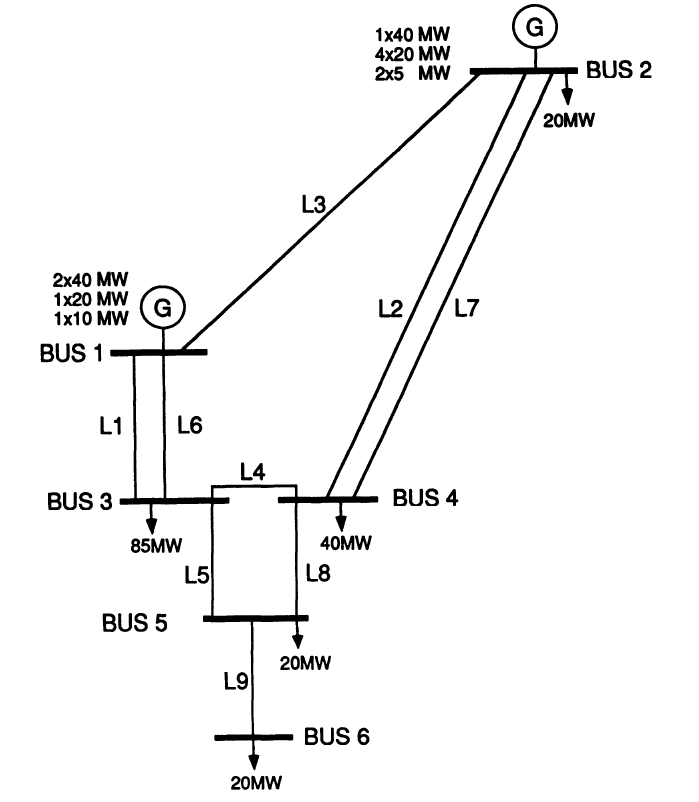
\includegraphics[width=\linewidth]{Figs/RBTS.png}
         \caption{Physical part. Adapted from~\cite{rbts}}
         \label{fig:RBTS-phys}
     \end{subfigure}
     \hfill
     \begin{subfigure}[b]{0.47\textwidth}
         \centering
         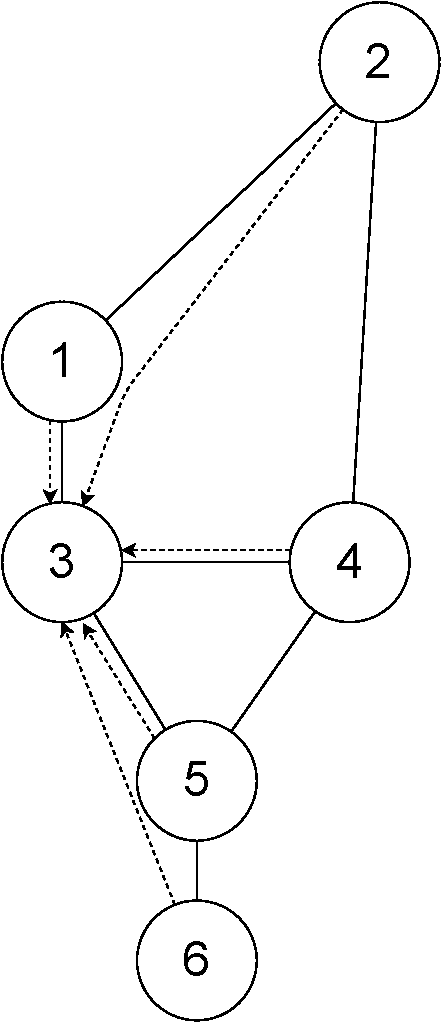
\includegraphics[width=0.5\linewidth]{Figs/RBTS_com.pdf}
         \caption{Communication infrastructure}
         \label{fig:RBTS-cyber}
     \end{subfigure}
\caption{Cyber-physical Roy Billinton test system (RBTS)}
\label{fig:RBTS}
\end{figure}

TSOs usually only use a fraction of the bandwidth provided by the OPGWs. They thus often choose to rent part of this bandwidth to ISPs~\cite[p110]{bookUK_OPGW}. The traffic used for the SPS should however not be in competition with the ISPs' traffic. This is achieved using quality of service (QoS) mechanisms such as weighted fair queuing. These mechanisms allow to guarantee a given amount of bandwidth for the SPS. Below, queuing theory is used to determine the minimum bandwidth to reserve for the SPS to stay under a maximum delay. Queuing theory is often used to study datagram networks, \ie networks where packets are routed individually such as in ISP networks. For critical applications, virtual circuit networks are an alternative. In these networks, reservations are made for the entire path between a source and a destination (emulating a direct copper cable between the two). They have higher setup costs and poorer scalability, but they offer higher reliability and maximum delay guarantees. The reliability of virtual circuit networks can be studied with classical reliability techniques and is not further discussed here.

The most common assumption in communication network traffic engineering is to consider that the distribution of arrivals is Poissonian~\cite{trafficBook}. In other words, it means that packets arrive with a constant mean rate and independently of the time elapsed since the last event. This assumption is very often valid in ISP networks due to the large number of independent inbound traffic sources\footnote{The validity of this hypothesis in the communication network of an SPS is discussed later in this section.}. Then, traffic load (or traffic intensity) of an element (router, firewall, etc.) is defined as:

\begin{equation}
\rho = \lambda/\mu
\end{equation}

\noindent where \(\lambda\) is the arrival rate of packets in the element [packets/s], and \(\mu\) is the processing rate of the element [packets/s]. Then, from the Poisson assumption, a well-known result from queuing theory~\cite{trafficBook} is that the average number of packets in the queue of the element is given by\footnote{Assuming a steady-state system, infinite buffer size, and \(\rho \leq 1\)}:

\begin{equation}
N = \frac{\rho}{1-\rho}
\end{equation}

We can then use Little's law~\cite{littleLaw} that states that the average queuing time \(t_q\) [s] spent by a packet in a system is given by:

\begin{equation}
\label{eq:little}
t_q = N/\lambda
\end{equation}

(Little's law is valid for any stationary system, \eg a single queue or a complex network.) It is also interesting to decompose \(t_q\) into the waiting time \(t_w\) and the processing time \(t_s = \frac{1}{\mu}\). For this, one can simply observe that when a packet arrives in a queue, it must wait for the average \(N\) packets already present to be processed. So,

\begin{equation}
\label{eq:t_w}
t_w = N t_s
\end{equation}

Equations~(\ref{eq:little}) and~(\ref{eq:t_w}) imply that,

\begin{equation}
t_w = \frac{\rho}{1-\rho} t_s
\end{equation}

\noindent and

\begin{equation}
\label{eq:final}
t_q = \frac{1}{1-\rho} t_s
\end{equation}

Equation~(\ref{eq:final}) is plotted in Fig~\ref{fig:queuing}. This figure illustrates clearly the impact of congestion on delays. This figure shows that, in order to limit the waiting delay (and its derivative with respect to \(\rho\)), the network should be operated such that \(\rho\) is lower than 0.7 or even 0.5. (As a rule of thumb, for 1~Mbps of traffic, links should thus have 2~Mbps of bandwidth.)

\begin{figure}
\centering
\begin{tikzpicture}
\pgfplotsset{width=0.6\linewidth}
        % legend style={font=\footnotesize}}
\begin{axis}[
    xlabel={Traffic intensity},
    ylabel= {\(t_q/t_s\)},
    enlarge x limits=0,
    enlarge y limits=0,
    xmin = 0,
    xmax = 1,
    xtick distance = 0.2,
    ytick distance = 2,
    ymin = 0,
    ymax = 8,
    smooth,
   ]

  \addplot [name path=A, blue, no marks, domain=0:0.95] {1/(1-x)};
  \addplot [name path=B, black, no marks, dashed] {1};
  \addplot[blue, fill opacity=0.2] fill between[of=A and B];

  \addplot [red, no marks, dashed] coordinates {(0, 3.33333333) (0.7, 3.33333333)};
  \addplot [red, no marks, dashed] coordinates {(0.7, 0) (0.7, 3.33333333)};

  \node at (axis cs:0.73,1.1) [anchor=south west, text width=5em, align=right] {Excess overhead induced by queuing};

  \node at (axis cs:0.01,3.2) [anchor=north west] {Zone of normal operation};

\end{axis}
\end{tikzpicture}
\caption{Communication delays as a function of congestion}
\label{fig:queuing}
\end{figure}

This methodology is now illustrated on the RBTS. For this, it is assumed that each PMU generates 120~kbps of traffic (packets of 300 bytes~\cite{StandardC37-118-2} sent at 50~Hz), that 300~kbps is reserved in each link for the SPS, and that packets are routed to the shortest path as shown in Figure~\ref{fig:RBTS-cyber}. Also, the processing time of routers is assumed to be limited by the bandwidth of links, \ie is equal to the packet size divided by the bandwidth, so 8~ms. The traffic in each link is simply the sum of all traffics going through this link\footnote{For routers where multiple PMU influxes are merged, a Poisson distribution of arrivals can still be assumed thanks to the additivity of the Poisson distribution. Thanks to this additivity property, queuing theory can easily be applied in large networks.}. From this traffic, one can compute the traffic intensity and the average queuing time as done in Table~\ref{tab:delayLink}. Then, the average communication delay between a given PMU and the CC is simply given by the sum of the delays in the path between this PMU and the CC. Those delays are given in Table~\ref{tab:delayPMU}.

\begin{table}
\centering
\caption{Computation of the average time spent by a packet in a given link for a reserved bandwidth of 300~kbps}
\label{tab:delayLink}
\begin{tabular}{|l|l|l|l|l|}
\hline
\multicolumn{1}{|c|}{\textbf{Link}} &
  \multicolumn{1}{c|}{\textbf{Traffic}} &
  \multicolumn{1}{c|}{\textbf{\(\bm{\rho}\)}} &
  \multicolumn{1}{c|}{\textbf{\(\bm{N}\)}} &
  \multicolumn{1}{c|}{\textbf{\(\bm{t_q}\) [ms]}} \\ \hline
2-1 & 120~kbps & 0.4 & 0.67 & 13.3 \\ \hline
1-3 & 240~kbps & 0.8 & 4    & 40   \\ \hline
4-3 & 120~kbps & 0.4 & 0.67 & 13.3 \\ \hline
5-3 & 240~kbps & 0.8 & 4    & 40   \\ \hline
6-5 & 120~kbps & 0.4 & 0.67 & 13.3 \\ \hline
\end{tabular}
\end{table}

\begin{table}
\centering
\caption{Average communication delays between each PMU and the CC}
\label{tab:delayPMU}
\begin{tabular}{|l|l|}
\hline
\multicolumn{1}{|c|}{\textbf{PMU \#}} & \multicolumn{1}{c|}{\textbf{\(\bm{t_q}\) (ms)}} \\ \hline
1                                    & 40                                     \\ \hline
2                                    & 53.3                                   \\ \hline
4                                    & 13.3                                   \\ \hline
5                                    & 40                                     \\ \hline
6                                    & 53.3                                   \\ \hline
\end{tabular}
\end{table}

These delays can be compared with the maximum delay allowable for the SPS's actions. In this case, the SPS protects the system against angle stability issues by disconnecting a 20~MW generator at bus 2 when either line 2, 3 or 7 is lost. To maintain angle stability, the generator should be disconnected at most 173~ms after the line loss. To determine the maximum communication delay that satisfy this constraint, the other (constant) delays have to be subtracted from those 173~ms. The processing times in the PMUs and CC is taken as 5 and 10~ms respectively~\cite{SPS-Ciapessoni}. A 20~ms worst-case delay due to the sampling rate of 50~Hz is also considered. The circuit breaker of the generator is supposed to open in 60~ms~\cite{ESOcircuitBreakerDelay}. A constant 8~ms delay is considered for communication between the CC and the generator\footnote{Queuing theory could also be used to compute this delay, however as messages from the CC to the generator travel in the opposite direction as messages from PMUs to the CC, they do not affect each other (assuming full duplex links).}. The propagation delays (1~ms per 200~km for a refractive index of the communication medium of 1.5) are neglected. There is thus 70~ms remaining for the communication delays between the PMUs and the CC. One can then verify than the average delays in Table~\ref{tab:delayPMU} are lower than 70~ms. It is also possible to compute the probability of the delays being lower than 70~ms. This is however more complex, and discussed in traffic engineering textbooks~\cite{trafficBook}.

The computations above have been made assuming a Poisson distribution of arrivals. The PMUs however send packets at a deterministic and constant rate. The developments above are still useful because the merging of several influxes in larger network tends to produce Poisson distributions. Also, the above method will very often lead to conservative results. In this particular case, simulations in ns-3 resulted in communications delays of 8~ms (the processing time in one router) for PMUs 1, 4 and 5, and 16~ms (twice the above value) for PMUs 2 and 6. Finally, due to the small amount of traffic needed by the SPS (and its critical nature), it is inexpensive to have large margins. This is true even for large networks. For example, even if all 2700 substations operated by the French TSO (mostly at 225 and 400~kV level)~\cite{RTEsubstations} sent PMU packets (300 bytes~\cite{StandardC37-118-2}) at a sampling rate of 50~Hz, it only results in a total of 360~Mbps\footnote{In the future, the size of the packets might increase slightly due to the transition to IPv6 (20 bytes), additional information regarding substation equipment being included in the PMU traffic (a few dozens of bytes), and longer cryptographic headers (a few dozens of bytes).}.

% If the SPS makes use of demand response, it is also necessary to have a communication infrastructure between the CC (and/or the individual buses) and end-users. Due to high geographical dispersion of end-users, it is completely unrealistic for the TSO to build its own ICT infrastructure for this purpose. The TSO thus has to make service level agreements (SLAs) with distribution system operators (DSOs) or ISPs. The TSO defines the amount of necessary bandwidth and maximum delay, and the DSO or ISP then has to make sure that those constraints are satisfied (\eg using queuing theory, QoS, etc.).

\subsection{Impact of failure}
\label{sec:ICTfailure}

The impact of cyber failures is studied differently if the ICT infrastructure is owned by the TSO or by an ISP. In the first case, the TSO can simply perform the same analysis as in section~\ref{sec:ICTsizing} but considering that some links are failed. For example, after a failure of link 3-4, traffic from the PMU 4 will be redirected through path 4-5, 3-5 which will increase the traffic intensity and queuing delays along this path. A higher bandwidth is thus necessary to stay under the target delay when considering possible failures. Additionally, if simultaneous failures of communication links and power lines are considered (due to a common mode failure), an additional delay has to be considered for the rerouting of the traffic.

In the second case, cyber failures will usually have a lower impact. This is because ICP's networks are usually more meshed than TSO's grids. For example, the core network of BT (formerly British Telecom) consists of 8 inner core nodes that are fully linked to each other, and 12 outer nodes that are each connected to at least 3 core nodes~\cite{BTnetwork}. Also, in this case, it is the ISP and not the TSO that has to make sure the cyber failures have a limited impact on the performance of the ICT infrastructure. The service level agreement (SLA) should define to what level of reliability the ICT performance (\ie availability and delays) should be guaranteed. Carrier-grade lines are often leased with a reliability level of 99.999\% (\ie 5 minutes of total downtime per year).

\subsection{Monitoring ICT performance}
\label{sec:ICTmonitoring}

Even if the ICT infrastructure has been appropriately sized (or if this the responsibility has been outsourced to an ISP), it is still useful to monitor its performance and to verify that the delays are under a given bound. Indeed, delays could increase following failures, bugs, attacks, increase of the traffic, etc. When high delays are detected, the SPS should arm schemes that are less time critical (\eg disconnection additional generators or loads), or send an alarm to the operators such that they take preventive actions (\eg reduction of the production at bus 2).

Monitoring the communication delays between the PMUs and the CC is direct since the packets sent by PMUs are precisely time-tagged (PMUs' clock are synchronised via GPS). For other communications (\eg communication with the generator's circuit breaker), this generally is not possible. An alternative is to estimate communication delays from Round Trip Time (RTT) measurements. In other words, when the TSO sends a message to a given recipient, it measures the time that passed between sending the message and receiving the acknowledgement message from the recipient. Assuming a symmetric network, the one-way delay is half the RTT. Since the TSO might not always need to communicate with recipients, it is necessary to use so-called keep-alive messages to have a continuous monitoring of the RTT. RTT measurements are used very often in ICT networks. The RTT-based mechanism used by TCP as defined by the Internet Engineering Task Force standard~\cite{roundTripTime} is presented below for illustration. There are similar mechanisms in other communication protocols such as RTP (Real-Time Protocol).

In TCP, when an application sends a message, it expects to receive an acknowledgement from the recipient. If it does not receive one, it resends the message. The Retransmission TimeOut (RTO) is defined as the maximum time after which a sender considers that if it did not receive an acknowledgement signal, then its message was lost and must thus be resent. The RTO can thus be seen as an upper bound (with a good probability) of the RTT. As the RTT can vary in time (due to variability of the traffic, seasonal effects, attacks, etc.), a ``smoothed'' RTT is defined. Each time a new measurement R' of the RTT is made, the smoothed RTT is updated according to:
%
\begin{equation}\text{SRTT} = (1-\alpha)\times\text{SRTT} + \alpha\times\text{R'}\end{equation}
%
where \(\alpha\) is a parameter often set to 0.125. To compute the RTO, a safety margin is added to the SRTT. This margin is higher when there are higher variations of the RTT. Mathematically, the variation of the RTT with is computed using,
%
\begin{equation}\text{RTTVAR} = (1-\beta)\times\text{RTTVAR} + \beta\times |\text{R'}-\text{SRTT}|\end{equation}
%
and the RTO as,
%
\begin{equation}\text{RTO} = \text{SRTT} + 4 \times \text{RTTVAR}\end{equation}
%
The recommended value for \(\beta\) is 0.25.


\subsection{Impact of traffic-based cyber-attacks}
\label{sec:ICTtrafficAttack}

The impact of cyber-attacks is usually classified into three categories: confidentiality, integrity and availability. Loss of confidentiality has no direct impact on the power system. It must be addressed through the use of classical cryptography. Attacks on integrity (\ie attacks that modify the data that is exchanged between different nodes) can cause wrong control actions either by directly injection/modifying control messages, or by modifying the measurements that are necessary to perform control actions. One advantage of using a state-estimation-based SPS is that it makes False Data Injection Attacks (FDIAs) more difficult. This is because the state estimator is based on a least square method. Measurements that have a high residual can thus be disregarded. This reduces the size of the set of possible successful attacks. There is a large body of literature on FDIAs (see \eg the review papers~\cite{FDIAreview, FDIAreview2}). Specific cryptography techniques can also be used to protect integrity of the data (\eg keyed hashing, authenticated encryption). The focus is thus placed on availability attacks in this section.

An example of availability attack is the Denial of Service (DoS) attack. In its most simple form, it is a volumetric attack that consists in exhausting computer resources by sending large amounts of redundant packets. More complex types of DoS attacks (\eg reflector-based attacks) exist but they have the same overall effect. The effect can intuitively be seen as a shift to the right in Figure~\ref{fig:queuing}. When small to medium amounts of traffic (compared to the available processing capacity of the system) are injected, it results in an increase of delays. When the total arrival rate is larger than the processing capacity of the system, then most packets are dropped; this is the most common case. QoS mechanisms can defend against DoS attacks, but they have to not only reserve bandwidth but also buffers. Other mitigation measures are discussed in dedicated literature.

The high amount of traffic caused by DoS attacks makes them easy to detect. They can thus often be mitigated automatically and relatively quickly. Such attack will thus only have physical consequences if the attacker manages to launch it just before an SPS action is needed. An attacker might thus prefer to use more ``subtle'' attacks to be less easily detected but still have an impact on the performance of the SPS. For example, if an attacker is able to take control of a router, he can then drop arbitrary packets instead of sending them to their original destination. This will have a different impact depending on the protocols that are used. The IEEE C37.118.2 standards recommends UDP (\ie no retransmission of lost packets) for the traffic coming from PMUs and TCP (\ie packets resent until an acknowledgement message is received) for the control traffic (from the CC)~\cite{StandardC37-118-2}.

If the attacker is unable to decrypt the packets going through the router he hijacked, he might choose to simply drops half the packets he receives. Since UDP is used, it means that half the data will no longer reach the CC. For example, if the router 1 (from Figure~\ref{fig:RBTS-cyber}) is attacked, then measurements from either bus 1 or 2 will be unavailable. In this case, only one measurement is lost. The state estimation algorithm can thus still compute the state of the whole system. However, in a real-scale system, individual routers (especially those near the CC) would see more measurements. It is thus possible to lose observability on part of the grid (standard methods for observability analysis can be used, \eg~\cite{SEbook}). Control messages on the other hand should never be completely missed, but they might need to be sent several times before being actually received. This introduces additional delays, and it would thus be useful to use a lower retransmission time than what is defined in~\cite{roundTripTime}.

If the attacker is able to decrypt the packets, he can cause more harm by dropping specific packets. The attacker could for example specifically drop disconnection messages that are sent to the generators. This basically renders the SPS out of service and a blackout could thus occur in case an action of the SPS is needed. The SPS considered here only has to operate for faults on lines 2, 3 and 7 (and only for some system configurations), so about once per year. The risk caused by such attacks is thus limited. For larger systems that heavily rely on SPS for many different types of faults (\eg ref.~\cite{GeorgiaSPS} reported 4 operations of its SPS for the first 11 days of 2016), the risk would be higher. It is worth noting that the attacker does not necessarily need to decrypt the packets. A lot of information can be deduced from the non-encrypted headers of the packets (\eg from the source, destination, and protocol used).

\section{Perspectives}
\label{sec:SPSperspectives}

% The probabilistic dynamic security assessment methodology presented proposed in this thesis can theoretically be applied either in planning or in operation. However, computation time issues are more stringent in operation which requires additional considerations. A way to circumvent those issues could be to store the results of the security assessment (to be performed all year round). Then, during operation, results associated with similar operating conditions than the current conditions can be retrieved. A similar approach (although in a slightly different context) was proposed in~\cite{QimingChenThesis}. This is however out of scope of this thesis.

The probabilistic dynamic security assessment method proposed in this thesis can identify critical contingencies that contribute to a significant share of the total risk of blackouts and identify the operating conditions for which these contingencies are unsecure. Such information could be used to design SPSs to reduce this risk.

% Another perspective is to use a probabilistic security assessment to identify the critical issues that pose significant risk to the system and then to design SPSs to alleviate those issues.

\chapter{Co-simulation of power and ICT systems}
\label{ch:cosim}
\minitoc

\begin{tcolorbox}[width=\linewidth, sharp corners=all,
    colback=white!80!black,
    colframe=white!80!black]
This chapter is partly based on the following publication:
\begin{itemize}
    \item \fullcite{Cosim}
\end{itemize}
\end{tcolorbox}

As mentioned in appendix~\ref{ch:SPS}, a possible approach to model cyber-physical systems, i.e. system that consist of a ``physical'' part (in this case, a power grid) and a ``cyber'' part (i.e. ICT (information and communication technology) systems) that both act on each others, is through the use of co-simulations\footnote{Co-simulation can also refer to the simulation of part of a power system with RMS tools and part with EMT tools. This is however not the topic of this chapter.}. When performing co-simulations, both parts of the system are modelled using two separate simulators (e.g. \Dynawo{} for the physical part, and ns-3 for the cyber part) that are then run together. The advantage of co-simulation is that both parts can be easily modelled using dedicated simulators (with standard libraries, solvers, etc.), but the drawback is that additional work is needed to make the two simulators run together. Indeed, the two simulators need to stay synchronised and exchange information about what is currently happening in both simulators (in order to model the interactions between the cyber and physical parts).

Before talking about time synchronisation of simulators, it can be noted that ICT and power system simulators have a different concept of time. Indeed, power system simulators work by solving a set of differential-algebraic equations (DAEs) that model the behaviour of the grid. Time is thus seen as a continuous variable (as the grid continuously evolves), although when numerically solving the DAEs, time will be discretised using a fixed or variable time step. On the other hand, ICT simulators are ``event-based'' which means that the state of the system only changes following events, and \emph{nothing} occurs in between.

To illustrate this, let's consider a very simple ICT system consisting of two nodes sending a message back-and-forth between each other through a communication link that has a 10ms propagation delay. Let's assume that the simulation starts with node 1 sending the message to node 2 at \(t=0ms\). At the start of the simulation, the event queue of the simulator thus contains a single event ``Node 1 sends a message at \(t=0ms\)''. The simulator then simulates this event, removes it from the queue, and creates a new event ``Node 2 receives a message at \(t=10ms\)''. The simulator then proceeds to this new event, removes it from the queue and creates a third event ``Node 2 sends a message at \(t=10ms\)''. The simulator continues like this until the event queue is empty or until \(t\) reaches the maximum simulation time.

Due to these differences between physical and cyber simulators, multiple approaches have been defined to synchronise them as discussed in~\cite{CosimFigure}. The most common approaches are illustrated in Figure~\ref{fig:Cosim}. The most straightforward approach consists in synchronising the simulators at predefined time intervals as shown in Figure~\ref{fig:CosimPointBased} and is referred to as point-based synchronisation. In other words, each time a simulator reaches a synchronisation point, it waits for the other simulator to also reach this point, then the two simulators exchange data about what occurred since the last synchronisation, and go back to simulating separately until the next synchronisation point. The drawback of this method is that when something happens in a simulator, the other is not made aware of it until the next synchronisation step. Events are thus perceived as ``delayed'' by the other simulator.

\begin{figure}
\centering
\subfloat[Point-based synchronisation]{%
\label{fig:CosimPointBased}
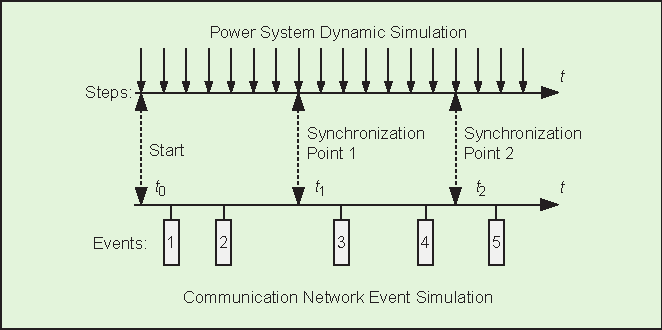
\includegraphics[width=0.7\linewidth]{Figs/CosimPointBased.pdf}
} \\ \vspace*{0.5cm} % \hfill
\subfloat[Event-based synchronisation]{%
\label{fig:CosimEventBased}
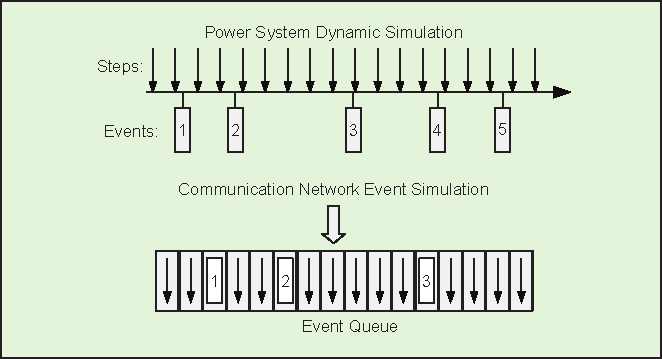
\includegraphics[width=0.7\linewidth]{Figs/CosimEventBased.pdf}
}
\caption{Main synchronisation techniques for co-simulation of cyber-physical systems~\cite{CosimFigure}}
\label{fig:Cosim}
\end{figure}

The second most common approach is the event-based synchronisation method illustrated in Figure~\ref{fig:CosimEventBased}. In this approach, time steps of the power system simulators and events in the cyber simulator are merged in a global event queue and the simulators are synchronised at each step of the global event queue (i.e. at each time step of the power system simulator, and for each event in the cyber simulator). The advantage of this method is that simulators are directly made aware when something occurs in the second simulator. It has however two important drawbacks. The first is that it is difficult to implement for power system simulators with variable integration time steps. Indeed, such simulators cannot say in advance what will be their next time step as it depends on zero-crossings and on numerical convergence. So complex rollback mechanisms must be implemented to account for cases where the power system simulator time step is smaller than predicted.

The second important drawback is that ICT simulators tend to generate events at a very fast rate (sub-millisecond rate or even lower) compared to the timescales of interest in power systems. Consider for example the test case shown in Figure~\ref{fig:IEEE_PMU} consisting of the standard IEEE 39-bus test system but equipped with a phasor measurement unit (PMU)-based state estimator. In this system, PMUs are installed at each bus and send measurements to phasor data concentrators (PDCs) every 30 times per second (the IEEE 39-bus system is US-based and is thus considered to be operated at 60~Hz in this chapter). PDCs aggregate this data and forward it to a super PDC (SPDC) that perform the state estimation and potentially initiate automatic corrective actions based on the state of the system.

\begin{figure}
\centering
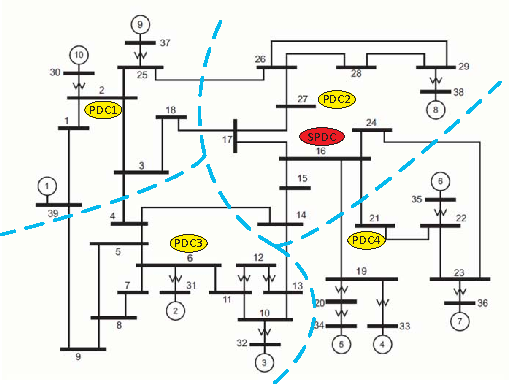
\includegraphics[width=0.6\linewidth]{Figs/IEEE39-PMU.pdf}
\caption{IEEE 39-bus test system with an all-PMU state estimator~\cite{GECOtestcase}}
\label{fig:IEEE_PMU}
\end{figure}

In this case, there are 39 PMUs that send messages to the communication network 30 times per second. If we take as a rough estimate that there are in average 3 hops between a PMU and the SPDC, this results in 3500 events and thus 3500 synchronisation steps per second, or in average, a synchronisation step every 0.3ms. Synchronisation steps would be even more frequent for larger systems. However, there is no point to have such frequent synchronisations as power system dynamics (at least the ones considered when using RMS simulators) are significantly slower.

The point-based synchronisation technique should thus be used in the majority of cases. For this approach, Table~\ref{tab:CosimComputationTime} analyses the impact of the co-simulation time step (i.e. how often the simulators are synchronised) on the total computation time for the above test case. The computation time is 4s when using a very large co-simulation time step (5000ms, effectively never synchronising the two simulators) and 16s, four times more, when using a very small step of 1ms. And actually, this increase in computation time is mostly due to the fact that a smaller co-simulation time step forces the power system simulator to use a smaller integration time step (the power system cannot use a 1s integration time step if synchronisations are performed every millisecond). Computations have been performed using a standard laptop CPU (AMD 4500U) and are significantly faster than the 20~minutes taken for a similar system in~\cite{GECOcomputationTime}. The reason for this is simply due to a better implementation. In~\cite{GECOcomputationTime}, authors use a closed-source power system simulator that does not have an interface designed to be used in a co-simulation. They are thus probably forced to stop the simulator, write power system to a file to disk, then to read this file and send the necessary values to the cyber simulator at each synchronisation time step. Our implementation connects \Dynawo{} and ns-3 using HELICS~\cite{HELICS}, a co-simulation orchestrator that enables efficient data exchanges through RAM, and is thus significantly faster.

\begin{table}
\centering
\caption{Evolution of computation time with using self-consistent and co-simulation. The simulated time is 5s.}
\begin{tabular}{@{}ll@{}}
\toprule
Co-simulation time step (ms) & Computation time \\ \midrule
5000ms                       & 4s               \\
10ms                         & 7s               \\
1ms                          & 16s              \\ \bottomrule
\end{tabular}
\label{tab:CosimComputationTime}
\end{table}


% \bibliographystyle{IEEEtranURLdate}
% \bibliography{bib}
\printbibliography[heading=bibintoc, title=References]


% \let\clearpage\relax  % Don't end on a blank page

\end{document}
